\documentclass[twoside]{book}

% Packages required by doxygen
\usepackage{fixltx2e}
\usepackage{calc}
\usepackage{doxygen}
\usepackage[export]{adjustbox} % also loads graphicx
\usepackage{graphicx}
\usepackage[utf8]{inputenc}
\usepackage{makeidx}
\usepackage{multicol}
\usepackage{multirow}
\PassOptionsToPackage{warn}{textcomp}
\usepackage{textcomp}
\usepackage[nointegrals]{wasysym}
\usepackage[table]{xcolor}

% Font selection
\usepackage[T1]{fontenc}
\usepackage[scaled=.90]{helvet}
\usepackage{courier}
\usepackage{amssymb}
\usepackage{sectsty}
\renewcommand{\familydefault}{\sfdefault}
\allsectionsfont{%
  \fontseries{bc}\selectfont%
  \color{darkgray}%
}
\renewcommand{\DoxyLabelFont}{%
  \fontseries{bc}\selectfont%
  \color{darkgray}%
}
\newcommand{\+}{\discretionary{\mbox{\scriptsize$\hookleftarrow$}}{}{}}

% Page & text layout
\usepackage{geometry}
\geometry{%
  a4paper,%
  top=2.5cm,%
  bottom=2.5cm,%
  left=2.5cm,%
  right=2.5cm%
}
\tolerance=750
\hfuzz=15pt
\hbadness=750
\setlength{\emergencystretch}{15pt}
\setlength{\parindent}{0cm}
\setlength{\parskip}{3ex plus 2ex minus 2ex}
\makeatletter
\renewcommand{\paragraph}{%
  \@startsection{paragraph}{4}{0ex}{-1.0ex}{1.0ex}{%
    \normalfont\normalsize\bfseries\SS@parafont%
  }%
}
\renewcommand{\subparagraph}{%
  \@startsection{subparagraph}{5}{0ex}{-1.0ex}{1.0ex}{%
    \normalfont\normalsize\bfseries\SS@subparafont%
  }%
}
\makeatother

% Headers & footers
\usepackage{fancyhdr}
\pagestyle{fancyplain}
\fancyhead[LE]{\fancyplain{}{\bfseries\thepage}}
\fancyhead[CE]{\fancyplain{}{}}
\fancyhead[RE]{\fancyplain{}{\bfseries\leftmark}}
\fancyhead[LO]{\fancyplain{}{\bfseries\rightmark}}
\fancyhead[CO]{\fancyplain{}{}}
\fancyhead[RO]{\fancyplain{}{\bfseries\thepage}}
\fancyfoot[LE]{\fancyplain{}{}}
\fancyfoot[CE]{\fancyplain{}{}}
\fancyfoot[RE]{\fancyplain{}{\bfseries\scriptsize Generated by Doxygen }}
\fancyfoot[LO]{\fancyplain{}{\bfseries\scriptsize Generated by Doxygen }}
\fancyfoot[CO]{\fancyplain{}{}}
\fancyfoot[RO]{\fancyplain{}{}}
\renewcommand{\footrulewidth}{0.4pt}
\renewcommand{\chaptermark}[1]{%
  \markboth{#1}{}%
}
\renewcommand{\sectionmark}[1]{%
  \markright{\thesection\ #1}%
}

% Indices & bibliography
\usepackage{natbib}
\usepackage[titles]{tocloft}
\setcounter{tocdepth}{3}
\setcounter{secnumdepth}{5}
\makeindex

% Hyperlinks (required, but should be loaded last)
\usepackage{ifpdf}
\ifpdf
  \usepackage[pdftex,pagebackref=true]{hyperref}
\else
  \usepackage[ps2pdf,pagebackref=true]{hyperref}
\fi
\hypersetup{%
  colorlinks=true,%
  linkcolor=blue,%
  citecolor=blue,%
  unicode%
}

% Custom commands
\newcommand{\clearemptydoublepage}{%
  \newpage{\pagestyle{empty}\cleardoublepage}%
}

\usepackage{caption}
\captionsetup{labelsep=space,justification=centering,font={bf},singlelinecheck=off,skip=4pt,position=top}

%===== C O N T E N T S =====

\begin{document}

% Titlepage & ToC
\hypersetup{pageanchor=false,
             bookmarksnumbered=true,
             pdfencoding=unicode
            }
\pagenumbering{alph}
\begin{titlepage}
\vspace*{7cm}
\begin{center}%
{\Large M\+\_\+system }\\
\vspace*{1cm}
{\large Generated by Doxygen 1.8.14}\\
\end{center}
\end{titlepage}
\clearemptydoublepage
\pagenumbering{roman}
\tableofcontents
\clearemptydoublepage
\pagenumbering{arabic}
\hypersetup{pageanchor=true}

%--- Begin generated contents ---
\chapter{M\+\_\+system Fortran Library}
\label{index}\hypertarget{index}{}\hypertarget{index_Introduction}{}\section{Introduction}\label{index_Introduction}
system interface using C\+\_\+\+I\+S\+O\+\_\+\+B\+I\+N\+D\+I\+NG interface to common P\+O\+S\+IX routines

 
\chapter{Modules Index}
\section{Modules List}
Here is a list of all modules with brief descriptions\+:\begin{DoxyCompactList}
\item\contentsline{section}{\mbox{\hyperlink{namespacem__system}{m\+\_\+system}} \\*\subsubsection*{N\+A\+ME}

M\+\_\+system(3fm) -\/ \mbox{[}M\+\_\+system\+::\+I\+N\+T\+RO\mbox{]} Fortran interface to C system interface (L\+I\+C\+E\+N\+SE\+:PD) \subsubsection*{S\+Y\+N\+O\+P\+S\+IS}}{\pageref{namespacem__system}}{}
\end{DoxyCompactList}

\chapter{Data Type Index}
\section{Data Types List}
Here are the data types with brief descriptions\+:\begin{DoxyCompactList}
\item\contentsline{section}{\mbox{\hyperlink{interfacem__system_1_1c__flush}{m\+\_\+system\+::c\+\_\+flush}} }{\pageref{interfacem__system_1_1c__flush}}{}
\item\contentsline{section}{\mbox{\hyperlink{structm__system_1_1dirent__cygwin}{m\+\_\+system\+::dirent\+\_\+cygwin}} }{\pageref{structm__system_1_1dirent__cygwin}}{}
\item\contentsline{section}{\mbox{\hyperlink{structm__system_1_1dirent__systema}{m\+\_\+system\+::dirent\+\_\+systema}} }{\pageref{structm__system_1_1dirent__systema}}{}
\item\contentsline{section}{\mbox{\hyperlink{interfacem__system_1_1system__alarm}{m\+\_\+system\+::system\+\_\+alarm}} }{\pageref{interfacem__system_1_1system__alarm}}{}
\item\contentsline{section}{\mbox{\hyperlink{interfacem__system_1_1system__calloc}{m\+\_\+system\+::system\+\_\+calloc}} }{\pageref{interfacem__system_1_1system__calloc}}{}
\item\contentsline{section}{\mbox{\hyperlink{interfacem__system_1_1system__clock}{m\+\_\+system\+::system\+\_\+clock}} }{\pageref{interfacem__system_1_1system__clock}}{}
\item\contentsline{section}{\mbox{\hyperlink{interfacem__system_1_1system__errno}{m\+\_\+system\+::system\+\_\+errno}} \\*\subsubsection*{N\+A\+ME}

system\+\_\+errno(3f) -\/ \mbox{[}M\+\_\+system\mbox{]} C error return value (L\+I\+C\+E\+N\+SE\+:PD) \subsubsection*{S\+Y\+N\+O\+P\+S\+IS}}{\pageref{interfacem__system_1_1system__errno}}{}
\item\contentsline{section}{\mbox{\hyperlink{interfacem__system_1_1system__free}{m\+\_\+system\+::system\+\_\+free}} }{\pageref{interfacem__system_1_1system__free}}{}
\item\contentsline{section}{\mbox{\hyperlink{interfacem__system_1_1system__getegid}{m\+\_\+system\+::system\+\_\+getegid}} \\*\subsubsection*{N\+A\+ME}

system\+\_\+getegid(3f) -\/ \mbox{[}M\+\_\+system\+:Q\+U\+E\+RY\mbox{]} get the effective group ID (G\+ID) of current process from Fortran by calling getegid(3c) (L\+I\+C\+E\+N\+SE\+:PD) \subsubsection*{S\+Y\+N\+O\+P\+S\+IS}}{\pageref{interfacem__system_1_1system__getegid}}{}
\item\contentsline{section}{\mbox{\hyperlink{interfacem__system_1_1system__geteuid}{m\+\_\+system\+::system\+\_\+geteuid}} \\*\subsubsection*{N\+A\+ME}

system\+\_\+geteuid(3f) -\/ \mbox{[}M\+\_\+system\+:Q\+U\+E\+RY\mbox{]} get effective U\+ID of current process from Fortran by calling geteuid(3c) (L\+I\+C\+E\+N\+SE\+:PD) \subsubsection*{S\+Y\+N\+O\+P\+S\+IS}}{\pageref{interfacem__system_1_1system__geteuid}}{}
\item\contentsline{section}{\mbox{\hyperlink{interfacem__system_1_1system__getgid}{m\+\_\+system\+::system\+\_\+getgid}} \\*\subsubsection*{N\+A\+ME}

system\+\_\+getgid(3f) -\/ \mbox{[}M\+\_\+system\+:Q\+U\+E\+RY\mbox{]} get the real group ID (G\+ID) of current process from Fortran by calling getgid(3c) (L\+I\+C\+E\+N\+SE\+:PD) \subsubsection*{S\+Y\+N\+O\+P\+S\+IS}}{\pageref{interfacem__system_1_1system__getgid}}{}
\item\contentsline{section}{\mbox{\hyperlink{interfacem__system_1_1system__getpid}{m\+\_\+system\+::system\+\_\+getpid}} \\*\subsubsection*{N\+A\+ME}

system\+\_\+getpid(3f) -\/ \mbox{[}M\+\_\+system\+:Q\+U\+E\+RY\mbox{]} get P\+ID (process ID) of current process from Fortran by calling getpid(3c) (L\+I\+C\+E\+N\+SE\+:PD) \subsubsection*{S\+Y\+N\+O\+P\+S\+IS}}{\pageref{interfacem__system_1_1system__getpid}}{}
\item\contentsline{section}{\mbox{\hyperlink{interfacem__system_1_1system__getppid}{m\+\_\+system\+::system\+\_\+getppid}} \\*\subsubsection*{N\+A\+ME}

system\+\_\+getppid(3f) -\/ \mbox{[}M\+\_\+system\+:Q\+U\+E\+RY\mbox{]} get parent process ID (P\+P\+ID) of current process from Fortran by calling getppid(3c) (L\+I\+C\+E\+N\+SE\+:PD) \subsubsection*{S\+Y\+N\+O\+P\+S\+IS}}{\pageref{interfacem__system_1_1system__getppid}}{}
\item\contentsline{section}{\mbox{\hyperlink{interfacem__system_1_1system__getsid}{m\+\_\+system\+::system\+\_\+getsid}} \\*\subsubsection*{N\+A\+ME}

system\+\_\+getsid(3f) -\/ \mbox{[}M\+\_\+system\+:Q\+U\+E\+RY\mbox{]} get the process group ID of a session leader (L\+I\+C\+E\+N\+SE\+:PD) \subsubsection*{S\+Y\+N\+O\+P\+S\+IS}}{\pageref{interfacem__system_1_1system__getsid}}{}
\item\contentsline{section}{\mbox{\hyperlink{interfacem__system_1_1system__getuid}{m\+\_\+system\+::system\+\_\+getuid}} \\*\subsubsection*{N\+A\+ME}

system\+\_\+getuid(3f) -\/ \mbox{[}M\+\_\+system\+:Q\+U\+E\+RY\mbox{]} get real U\+ID of current process from Fortran by calling getuid(3c) (L\+I\+C\+E\+N\+SE\+:PD) \subsubsection*{S\+Y\+N\+O\+P\+S\+IS}}{\pageref{interfacem__system_1_1system__getuid}}{}
\item\contentsline{section}{\mbox{\hyperlink{interfacem__system_1_1system__initenv}{m\+\_\+system\+::system\+\_\+initenv}} }{\pageref{interfacem__system_1_1system__initenv}}{}
\item\contentsline{section}{\mbox{\hyperlink{interfacem__system_1_1system__kill}{m\+\_\+system\+::system\+\_\+kill}} \\*\subsubsection*{N\+A\+ME}

system\+\_\+kill(3f) -\/ \mbox{[}M\+\_\+system\mbox{]} send a signal to a process or a group of processes (L\+I\+C\+E\+N\+SE\+:PD) }{\pageref{interfacem__system_1_1system__kill}}{}
\item\contentsline{section}{\mbox{\hyperlink{interfacem__system_1_1system__malloc}{m\+\_\+system\+::system\+\_\+malloc}} }{\pageref{interfacem__system_1_1system__malloc}}{}
\item\contentsline{section}{\mbox{\hyperlink{interfacem__system_1_1system__memcpy}{m\+\_\+system\+::system\+\_\+memcpy}} }{\pageref{interfacem__system_1_1system__memcpy}}{}
\item\contentsline{section}{\mbox{\hyperlink{interfacem__system_1_1system__rand}{m\+\_\+system\+::system\+\_\+rand}} \\*\subsubsection*{N\+A\+ME}

system\+\_\+rand(3f) -\/ \mbox{[}M\+\_\+system\mbox{]} call pseudo-\/random number generator rand(3c) (L\+I\+C\+E\+N\+SE\+:PD) \subsubsection*{S\+Y\+N\+O\+P\+S\+IS}}{\pageref{interfacem__system_1_1system__rand}}{}
\item\contentsline{section}{\mbox{\hyperlink{interfacem__system_1_1system__realloc}{m\+\_\+system\+::system\+\_\+realloc}} }{\pageref{interfacem__system_1_1system__realloc}}{}
\item\contentsline{section}{\mbox{\hyperlink{interfacem__system_1_1system__setsid}{m\+\_\+system\+::system\+\_\+setsid}} \\*\subsubsection*{N\+A\+ME}

system\+\_\+setsid(3f) -\/ \mbox{[}M\+\_\+system\+:Q\+U\+E\+RY\mbox{]} create session and set the process group ID of a session leader (L\+I\+C\+E\+N\+SE\+:PD) \subsubsection*{S\+Y\+N\+O\+P\+S\+IS}}{\pageref{interfacem__system_1_1system__setsid}}{}
\item\contentsline{section}{\mbox{\hyperlink{interfacem__system_1_1system__srand}{m\+\_\+system\+::system\+\_\+srand}} \\*\subsubsection*{N\+A\+ME}

system\+\_\+srand(3f) -\/ \mbox{[}M\+\_\+system\mbox{]} set seed for pseudo-\/random number generator system\+\_\+rand(3f) (L\+I\+C\+E\+N\+SE\+:PD) }{\pageref{interfacem__system_1_1system__srand}}{}
\item\contentsline{section}{\mbox{\hyperlink{interfacem__system_1_1system__time}{m\+\_\+system\+::system\+\_\+time}} }{\pageref{interfacem__system_1_1system__time}}{}
\item\contentsline{section}{\mbox{\hyperlink{interfacem__system_1_1system__umask}{m\+\_\+system\+::system\+\_\+umask}} \\*\subsubsection*{N\+A\+ME}

system\+\_\+umask(3fp) -\/ \mbox{[}M\+\_\+system\mbox{]} set and get the file mode creation mask (L\+I\+C\+E\+N\+SE\+:PD) \subsubsection*{S\+Y\+N\+O\+P\+S\+IS}}{\pageref{interfacem__system_1_1system__umask}}{}
\end{DoxyCompactList}

\chapter{File Index}
\section{File List}
Here is a list of all files with brief descriptions\+:\begin{DoxyCompactList}
\item\contentsline{section}{/home/urbanjs/venus/\+V600/github/\+M\+\_\+system/src/\mbox{\hyperlink{C-M__system_8c}{C-\/\+M\+\_\+system.\+c}} }{\pageref{C-M__system_8c}}{}
\item\contentsline{section}{/home/urbanjs/venus/\+V600/github/\+M\+\_\+system/src/\mbox{\hyperlink{M__system_8f90}{M\+\_\+system.\+f90}} }{\pageref{M__system_8f90}}{}
\end{DoxyCompactList}

\chapter{Module Documentation}
\hypertarget{namespacem__system}{}\section{m\+\_\+system Module Reference}
\label{namespacem__system}\index{m\+\_\+system@{m\+\_\+system}}


\subsubsection*{N\+A\+ME}

M\+\_\+system(3fm) -\/ \mbox{[}M\+\_\+system\+::\+I\+N\+T\+RO\mbox{]} Fortran interface to C system interface (L\+I\+C\+E\+N\+SE\+:PD) \subsubsection*{S\+Y\+N\+O\+P\+S\+IS} 


\subsection*{Data Types}
\begin{DoxyCompactItemize}
\item 
interface \mbox{\hyperlink{interfacem__system_1_1c__flush}{c\+\_\+flush}}
\item 
type \mbox{\hyperlink{structm__system_1_1dirent__cygwin}{dirent\+\_\+cygwin}}
\item 
type \mbox{\hyperlink{structm__system_1_1dirent__systema}{dirent\+\_\+systema}}
\item 
interface \mbox{\hyperlink{interfacem__system_1_1system__alarm}{system\+\_\+alarm}}
\item 
interface \mbox{\hyperlink{interfacem__system_1_1system__calloc}{system\+\_\+calloc}}
\item 
interface \mbox{\hyperlink{interfacem__system_1_1system__clock}{system\+\_\+clock}}
\item 
interface \mbox{\hyperlink{interfacem__system_1_1system__errno}{system\+\_\+errno}}
\begin{DoxyCompactList}\small\item\em \subsubsection*{N\+A\+ME}

system\+\_\+errno(3f) -\/ \mbox{[}M\+\_\+system\mbox{]} C error return value (L\+I\+C\+E\+N\+SE\+:PD) \subsubsection*{S\+Y\+N\+O\+P\+S\+IS}\end{DoxyCompactList}\item 
interface \mbox{\hyperlink{interfacem__system_1_1system__free}{system\+\_\+free}}
\item 
interface \mbox{\hyperlink{interfacem__system_1_1system__getegid}{system\+\_\+getegid}}
\begin{DoxyCompactList}\small\item\em \subsubsection*{N\+A\+ME}

system\+\_\+getegid(3f) -\/ \mbox{[}M\+\_\+system\+:Q\+U\+E\+RY\mbox{]} get the effective group ID (G\+ID) of current process from Fortran by calling getegid(3c) (L\+I\+C\+E\+N\+SE\+:PD) \subsubsection*{S\+Y\+N\+O\+P\+S\+IS}\end{DoxyCompactList}\item 
interface \mbox{\hyperlink{interfacem__system_1_1system__geteuid}{system\+\_\+geteuid}}
\begin{DoxyCompactList}\small\item\em \subsubsection*{N\+A\+ME}

system\+\_\+geteuid(3f) -\/ \mbox{[}M\+\_\+system\+:Q\+U\+E\+RY\mbox{]} get effective U\+ID of current process from Fortran by calling geteuid(3c) (L\+I\+C\+E\+N\+SE\+:PD) \subsubsection*{S\+Y\+N\+O\+P\+S\+IS}\end{DoxyCompactList}\item 
interface \mbox{\hyperlink{interfacem__system_1_1system__getgid}{system\+\_\+getgid}}
\begin{DoxyCompactList}\small\item\em \subsubsection*{N\+A\+ME}

system\+\_\+getgid(3f) -\/ \mbox{[}M\+\_\+system\+:Q\+U\+E\+RY\mbox{]} get the real group ID (G\+ID) of current process from Fortran by calling getgid(3c) (L\+I\+C\+E\+N\+SE\+:PD) \subsubsection*{S\+Y\+N\+O\+P\+S\+IS}\end{DoxyCompactList}\item 
interface \mbox{\hyperlink{interfacem__system_1_1system__getpid}{system\+\_\+getpid}}
\begin{DoxyCompactList}\small\item\em \subsubsection*{N\+A\+ME}

system\+\_\+getpid(3f) -\/ \mbox{[}M\+\_\+system\+:Q\+U\+E\+RY\mbox{]} get P\+ID (process ID) of current process from Fortran by calling getpid(3c) (L\+I\+C\+E\+N\+SE\+:PD) \subsubsection*{S\+Y\+N\+O\+P\+S\+IS}\end{DoxyCompactList}\item 
interface \mbox{\hyperlink{interfacem__system_1_1system__getppid}{system\+\_\+getppid}}
\begin{DoxyCompactList}\small\item\em \subsubsection*{N\+A\+ME}

system\+\_\+getppid(3f) -\/ \mbox{[}M\+\_\+system\+:Q\+U\+E\+RY\mbox{]} get parent process ID (P\+P\+ID) of current process from Fortran by calling getppid(3c) (L\+I\+C\+E\+N\+SE\+:PD) \subsubsection*{S\+Y\+N\+O\+P\+S\+IS}\end{DoxyCompactList}\item 
interface \mbox{\hyperlink{interfacem__system_1_1system__getsid}{system\+\_\+getsid}}
\begin{DoxyCompactList}\small\item\em \subsubsection*{N\+A\+ME}

system\+\_\+getsid(3f) -\/ \mbox{[}M\+\_\+system\+:Q\+U\+E\+RY\mbox{]} get the process group ID of a session leader (L\+I\+C\+E\+N\+SE\+:PD) \subsubsection*{S\+Y\+N\+O\+P\+S\+IS}\end{DoxyCompactList}\item 
interface \mbox{\hyperlink{interfacem__system_1_1system__getuid}{system\+\_\+getuid}}
\begin{DoxyCompactList}\small\item\em \subsubsection*{N\+A\+ME}

system\+\_\+getuid(3f) -\/ \mbox{[}M\+\_\+system\+:Q\+U\+E\+RY\mbox{]} get real U\+ID of current process from Fortran by calling getuid(3c) (L\+I\+C\+E\+N\+SE\+:PD) \subsubsection*{S\+Y\+N\+O\+P\+S\+IS}\end{DoxyCompactList}\item 
interface \mbox{\hyperlink{interfacem__system_1_1system__initenv}{system\+\_\+initenv}}
\item 
interface \mbox{\hyperlink{interfacem__system_1_1system__kill}{system\+\_\+kill}}
\begin{DoxyCompactList}\small\item\em \subsubsection*{N\+A\+ME}

system\+\_\+kill(3f) -\/ \mbox{[}M\+\_\+system\mbox{]} send a signal to a process or a group of processes (L\+I\+C\+E\+N\+SE\+:PD) \end{DoxyCompactList}\item 
interface \mbox{\hyperlink{interfacem__system_1_1system__malloc}{system\+\_\+malloc}}
\item 
interface \mbox{\hyperlink{interfacem__system_1_1system__memcpy}{system\+\_\+memcpy}}
\item 
interface \mbox{\hyperlink{interfacem__system_1_1system__rand}{system\+\_\+rand}}
\begin{DoxyCompactList}\small\item\em \subsubsection*{N\+A\+ME}

system\+\_\+rand(3f) -\/ \mbox{[}M\+\_\+system\mbox{]} call pseudo-\/random number generator rand(3c) (L\+I\+C\+E\+N\+SE\+:PD) \subsubsection*{S\+Y\+N\+O\+P\+S\+IS}\end{DoxyCompactList}\item 
interface \mbox{\hyperlink{interfacem__system_1_1system__realloc}{system\+\_\+realloc}}
\item 
interface \mbox{\hyperlink{interfacem__system_1_1system__setsid}{system\+\_\+setsid}}
\begin{DoxyCompactList}\small\item\em \subsubsection*{N\+A\+ME}

system\+\_\+setsid(3f) -\/ \mbox{[}M\+\_\+system\+:Q\+U\+E\+RY\mbox{]} create session and set the process group ID of a session leader (L\+I\+C\+E\+N\+SE\+:PD) \subsubsection*{S\+Y\+N\+O\+P\+S\+IS}\end{DoxyCompactList}\item 
interface \mbox{\hyperlink{interfacem__system_1_1system__srand}{system\+\_\+srand}}
\begin{DoxyCompactList}\small\item\em \subsubsection*{N\+A\+ME}

system\+\_\+srand(3f) -\/ \mbox{[}M\+\_\+system\mbox{]} set seed for pseudo-\/random number generator system\+\_\+rand(3f) (L\+I\+C\+E\+N\+SE\+:PD) \end{DoxyCompactList}\item 
interface \mbox{\hyperlink{interfacem__system_1_1system__time}{system\+\_\+time}}
\item 
interface \mbox{\hyperlink{interfacem__system_1_1system__umask}{system\+\_\+umask}}
\begin{DoxyCompactList}\small\item\em \subsubsection*{N\+A\+ME}

system\+\_\+umask(3fp) -\/ \mbox{[}M\+\_\+system\mbox{]} set and get the file mode creation mask (L\+I\+C\+E\+N\+SE\+:PD) \subsubsection*{S\+Y\+N\+O\+P\+S\+IS}\end{DoxyCompactList}\end{DoxyCompactItemize}
\subsection*{Functions/\+Subroutines}
\begin{DoxyCompactItemize}
\item 
logical function, public \mbox{\hyperlink{namespacem__system_a4687a363acbb7084a51bc77844789275}{system\+\_\+access}} (pathname, amode)
\begin{DoxyCompactList}\small\item\em \subsubsection*{N\+A\+ME}

system\+\_\+access(3f) -\/ \mbox{[}M\+\_\+system\mbox{]} checks accessibility or existence of a pathname (L\+I\+C\+E\+N\+SE\+:PD) \end{DoxyCompactList}\item 
logical function, public \mbox{\hyperlink{namespacem__system_a83a121ba0b525210b5217565569ef350}{system\+\_\+utime}} (pathname, times)
\begin{DoxyCompactList}\small\item\em \subsubsection*{N\+A\+ME}

system\+\_\+utime(3f) -\/ \mbox{[}M\+\_\+system\mbox{]} set file access and modification times (L\+I\+C\+E\+N\+SE\+:PD) \end{DoxyCompactList}\item 
character(len=\+:) function, allocatable, public \mbox{\hyperlink{namespacem__system_a70bbfa0a0be084b9717cbc04408041fc}{system\+\_\+realpath}} (input)
\begin{DoxyCompactList}\small\item\em \subsubsection*{N\+A\+ME}

system\+\_\+realpath(3f) -\/ \mbox{[}M\+\_\+system\mbox{]} call realpath(3c) to resolve a pathname (L\+I\+C\+E\+N\+SE\+:PD) \subsubsection*{S\+Y\+N\+O\+P\+S\+IS}\end{DoxyCompactList}\item 
logical function, public \mbox{\hyperlink{namespacem__system_af6eb5074fe74552bc7a5e7d00f459087}{system\+\_\+issock}} (pathname)
\begin{DoxyCompactList}\small\item\em \subsubsection*{N\+A\+ME}

system\+\_\+issock(3f) -\/ \mbox{[}M\+\_\+system\mbox{]} checks if argument is a socket (L\+I\+C\+E\+N\+SE\+:PD) \end{DoxyCompactList}\item 
logical function, public \mbox{\hyperlink{namespacem__system_acbcaa0c5075ca103815f441ee410e1a3}{system\+\_\+isfifo}} (pathname)
\begin{DoxyCompactList}\small\item\em \subsubsection*{N\+A\+ME}

system\+\_\+isfifo(3f) -\/ \mbox{[}M\+\_\+system\mbox{]} checks if argument is a fifo -\/ named pipe (L\+I\+C\+E\+N\+SE\+:PD) \end{DoxyCompactList}\item 
logical function, public \mbox{\hyperlink{namespacem__system_a12a948fa4aacda084a538ae3a5ae3cc6}{system\+\_\+ischr}} (pathname)
\begin{DoxyCompactList}\small\item\em \subsubsection*{N\+A\+ME}

system\+\_\+ischr(3f) -\/ \mbox{[}M\+\_\+system\mbox{]} checks if argument is a character device (L\+I\+C\+E\+N\+SE\+:PD) \end{DoxyCompactList}\item 
logical function, public \mbox{\hyperlink{namespacem__system_a127bdd84ccd4b52f3f29abbc56af029b}{system\+\_\+isreg}} (pathname)
\begin{DoxyCompactList}\small\item\em \subsubsection*{N\+A\+ME}

system\+\_\+isreg(3f) -\/ \mbox{[}M\+\_\+system\mbox{]} checks if argument is a regular file (L\+I\+C\+E\+N\+SE\+:PD) \end{DoxyCompactList}\item 
logical function, public \mbox{\hyperlink{namespacem__system_ab05694cc3d76a3ecc87e4b4490c4c217}{system\+\_\+islnk}} (pathname)
\begin{DoxyCompactList}\small\item\em \subsubsection*{N\+A\+ME}

system\+\_\+islnk(3f) -\/ \mbox{[}M\+\_\+system\mbox{]} checks if argument is a link (L\+I\+C\+E\+N\+SE\+:PD) \end{DoxyCompactList}\item 
logical function, public \mbox{\hyperlink{namespacem__system_a791fa587005ec07cbcd7b0045ee6f43f}{system\+\_\+isblk}} (pathname)
\begin{DoxyCompactList}\small\item\em \subsubsection*{N\+A\+ME}

system\+\_\+isblk(3f) -\/ \mbox{[}M\+\_\+system\mbox{]} checks if argument is a block device (L\+I\+C\+E\+N\+SE\+:PD) \end{DoxyCompactList}\item 
logical function, public \mbox{\hyperlink{namespacem__system_a3353c1cff032fcfe2985a69f10038ddd}{system\+\_\+chown}} (dirname, owner, group)
\begin{DoxyCompactList}\small\item\em \subsubsection*{N\+A\+ME}

system\+\_\+chown(3f) -\/ \mbox{[}M\+\_\+system\mbox{]} change file owner and group (L\+I\+C\+E\+N\+SE\+:PD) \end{DoxyCompactList}\item 
logical function, public \mbox{\hyperlink{namespacem__system_ad097988a031e64b4f21f856cf45c9c73}{system\+\_\+isdir}} (dirname)
\begin{DoxyCompactList}\small\item\em \subsubsection*{N\+A\+ME}

system\+\_\+isdir(3f) -\/ \mbox{[}M\+\_\+system\mbox{]} checks if argument is a directory path (L\+I\+C\+E\+N\+SE\+:PD) \end{DoxyCompactList}\item 
subroutine, public \mbox{\hyperlink{namespacem__system_a257d2b8987db850bc686507f19ccbe4a}{system\+\_\+cpu\+\_\+time}} (total, user, system)
\begin{DoxyCompactList}\small\item\em \subsubsection*{N\+A\+ME}

system\+\_\+cpu\+\_\+time(3f) -\/ \mbox{[}M\+\_\+system\mbox{]} get processor time by calling times(3c) (L\+I\+C\+E\+N\+SE\+:PD) \end{DoxyCompactList}\item 
integer function, public \mbox{\hyperlink{namespacem__system_aa77d9c9ae68750f515ba3d04d022c43c}{system\+\_\+link}} (oldname, newname)
\begin{DoxyCompactList}\small\item\em \subsubsection*{N\+A\+ME}

system\+\_\+link(3f) -\/ \mbox{[}M\+\_\+system\mbox{]} link one file to another file relative to two directory file descriptors (L\+I\+C\+E\+N\+SE\+:PD) \end{DoxyCompactList}\item 
integer function, public \mbox{\hyperlink{namespacem__system_a14ce0b9177815bc357dbdf3778687bb7}{system\+\_\+unlink}} (fname)
\begin{DoxyCompactList}\small\item\em \subsubsection*{N\+A\+ME}

system\+\_\+unlink(3f) -\/ \mbox{[}M\+\_\+system\mbox{]} remove a directory entry relative to directory file descriptor (L\+I\+C\+E\+N\+SE\+:PD) \end{DoxyCompactList}\item 
integer function, public \mbox{\hyperlink{namespacem__system_a04fd02e6f5ce2f8ecdfb577e1490feba}{system\+\_\+setumask}} (umask\+\_\+value)
\begin{DoxyCompactList}\small\item\em \subsubsection*{N\+A\+ME}

system\+\_\+setumask(3f) -\/ \mbox{[}M\+\_\+system\mbox{]} set the file mode creation umask (L\+I\+C\+E\+N\+SE\+:PD) \subsubsection*{S\+Y\+N\+O\+P\+S\+IS}\end{DoxyCompactList}\item 
integer function, public \mbox{\hyperlink{namespacem__system_aa9ca951be39d2ea738d627cf42c00ddd}{system\+\_\+getumask}} ()
\begin{DoxyCompactList}\small\item\em \subsubsection*{N\+A\+ME}

system\+\_\+getumask(3f) -\/ \mbox{[}M\+\_\+system\mbox{]} get current umask (L\+I\+C\+E\+N\+SE\+:PD) \subsubsection*{S\+Y\+N\+O\+P\+S\+IS}\end{DoxyCompactList}\item 
subroutine, public \mbox{\hyperlink{namespacem__system_afae451a1fc5432274dc1f75a364051b4}{system\+\_\+perror}} (prefix)
\begin{DoxyCompactList}\small\item\em \subsubsection*{N\+A\+ME}

perror(3f) -\/ \mbox{[}M\+\_\+system\mbox{]} print error message for last C error on stderr (L\+I\+C\+E\+N\+SE\+:PD) \subsubsection*{S\+Y\+N\+O\+P\+S\+IS}\end{DoxyCompactList}\item 
subroutine, public \mbox{\hyperlink{namespacem__system_a47746b670cb21bae0957c9bb2bccf209}{system\+\_\+chdir}} (path, err)
\begin{DoxyCompactList}\small\item\em \subsubsection*{N\+A\+ME}

system\+\_\+chdir(3f) -\/ \mbox{[}M\+\_\+system\mbox{]} call chdir(3c) from Fortran to change working directory (L\+I\+C\+E\+N\+SE\+:PD) \subsubsection*{S\+Y\+N\+O\+P\+S\+IS}\end{DoxyCompactList}\item 
integer(c\+\_\+int) function, public \mbox{\hyperlink{namespacem__system_a730ae64294e3cd73bde8f0c63cdf9972}{system\+\_\+remove}} (path)
\begin{DoxyCompactList}\small\item\em \subsubsection*{N\+A\+ME}

system\+\_\+remove(3f) -\/ \mbox{[}M\+\_\+system\mbox{]} call remove(3c) to remove file (L\+I\+C\+E\+N\+SE\+:PD) \subsubsection*{S\+Y\+N\+O\+P\+S\+IS}\end{DoxyCompactList}\item 
integer function, public \mbox{\hyperlink{namespacem__system_adfbaf3d17790da9ba0c520683d5b8003}{system\+\_\+rename}} (input, output)
\begin{DoxyCompactList}\small\item\em \subsubsection*{N\+A\+ME}

system\+\_\+rename(3f) -\/ \mbox{[}M\+\_\+system\mbox{]} call rename(3c) to rename a system file (L\+I\+C\+E\+N\+SE\+:PD) \subsubsection*{S\+Y\+N\+O\+P\+S\+IS}\end{DoxyCompactList}\item 
integer function, public \mbox{\hyperlink{namespacem__system_ace9ce0c8a9c8341a76b8903cd2390ce3}{system\+\_\+chmod}} (filename, mode)
\begin{DoxyCompactList}\small\item\em \subsubsection*{N\+A\+ME}

system\+\_\+chmod(3f) -\/ \mbox{[}M\+\_\+system\mbox{]} call chmod(3c) to change permission mode of a file relative to directory file descriptor (L\+I\+C\+E\+N\+SE\+:PD) \subsubsection*{S\+Y\+N\+O\+P\+S\+IS}\end{DoxyCompactList}\item 
subroutine, public \mbox{\hyperlink{namespacem__system_a5a32db818a9ffb0a4ea724e95356c560}{system\+\_\+getcwd}} (output, ierr)
\begin{DoxyCompactList}\small\item\em \subsubsection*{N\+A\+ME}

system\+\_\+getcwd(3f) -\/ \mbox{[}M\+\_\+system\mbox{]} call getcwd(3c) to get the pathname of the current working directory (L\+I\+C\+E\+N\+SE\+:PD) \subsubsection*{S\+Y\+N\+O\+P\+S\+IS}\end{DoxyCompactList}\item 
integer(c\+\_\+int) function, public \mbox{\hyperlink{namespacem__system_a21fd3e1ccd50cef6adc539ef3d7a9836}{system\+\_\+rmdir}} (dirname)
\begin{DoxyCompactList}\small\item\em \subsubsection*{N\+A\+ME}

system\+\_\+rmdir(3f) -\/ \mbox{[}M\+\_\+system\mbox{]} call rmdir(3c) to remove empty directories (L\+I\+C\+E\+N\+SE\+:PD) \end{DoxyCompactList}\item 
integer function, public \mbox{\hyperlink{namespacem__system_ab2d95258ee26b85a0283538880775475}{system\+\_\+mkfifo}} (pathname, mode)
\begin{DoxyCompactList}\small\item\em \subsubsection*{N\+A\+ME}

system\+\_\+mkfifo(3f) -\/ \mbox{[}M\+\_\+system\mbox{]} make a F\+I\+FO special file relative to directory file descriptor (L\+I\+C\+E\+N\+SE\+:PD) \subsubsection*{S\+Y\+N\+O\+P\+S\+IS}\end{DoxyCompactList}\item 
integer function, public \mbox{\hyperlink{namespacem__system_a084d644c236d22af2cc75c6e48fd6e96}{system\+\_\+mkdir}} (dirname, mode)
\begin{DoxyCompactList}\small\item\em \subsubsection*{N\+A\+ME}

system\+\_\+mkdir(3f) -\/ \mbox{[}M\+\_\+system\mbox{]} call mkdir(3c) to create a new directory (L\+I\+C\+E\+N\+SE\+:PD) \subsubsection*{S\+Y\+N\+O\+P\+S\+IS}\end{DoxyCompactList}\item 
subroutine, public \mbox{\hyperlink{namespacem__system_a622cc67c03e8cdea1d4c2430bb36081b}{system\+\_\+opendir}} (dirname, dir, ierr)
\begin{DoxyCompactList}\small\item\em \subsubsection*{N\+A\+ME}

system\+\_\+opendir(3f) -\/ \mbox{[}M\+\_\+system\mbox{]} open directory stream by calling opendir(3c) (L\+I\+C\+E\+N\+SE\+:PD) \subsubsection*{S\+Y\+N\+O\+P\+S\+IS}\end{DoxyCompactList}\item 
subroutine, public \mbox{\hyperlink{namespacem__system_a983df5b2d7cb5842d69c4a31829403e0}{system\+\_\+readdir}} (dir, filename, ierr)
\begin{DoxyCompactList}\small\item\em \subsubsection*{N\+A\+ME}

system\+\_\+readdir(3f) -\/ \mbox{[}M\+\_\+system\mbox{]} read a directory using readdir(3c) (L\+I\+C\+E\+N\+SE\+:PD) \subsubsection*{S\+Y\+N\+O\+P\+S\+IS}\end{DoxyCompactList}\item 
subroutine, public \mbox{\hyperlink{namespacem__system_a3ffe757195ade8052e8acabd196ee3ca}{system\+\_\+rewinddir}} (dir)
\begin{DoxyCompactList}\small\item\em \subsubsection*{N\+A\+ME}

system\+\_\+rewinddir(3f) -\/ \mbox{[}M\+\_\+system\mbox{]} call rewinddir(3c) to rewind directory stream (L\+I\+C\+E\+N\+SE\+:PD) \subsubsection*{S\+Y\+N\+O\+P\+S\+IS}\end{DoxyCompactList}\item 
subroutine, public \mbox{\hyperlink{namespacem__system_acd442b52c64fc50482bc08b0ac8a50d1}{system\+\_\+closedir}} (dir, ierr)
\begin{DoxyCompactList}\small\item\em \subsubsection*{N\+A\+ME}

system\+\_\+closedir(3f) -\/ \mbox{[}M\+\_\+system\mbox{]} close a directory stream by calling closedir(3c) (L\+I\+C\+E\+N\+SE\+:PD) \subsubsection*{S\+Y\+N\+O\+P\+S\+IS}\end{DoxyCompactList}\item 
subroutine, public \mbox{\hyperlink{namespacem__system_af0c9df8e59cac9cd617cd1e20448ea7d}{system\+\_\+putenv}} (string, err)
\begin{DoxyCompactList}\small\item\em \subsubsection*{N\+A\+ME}

system\+\_\+putenv(3f) -\/ \mbox{[}M\+\_\+system\+:E\+N\+V\+I\+R\+O\+N\+M\+E\+NT\mbox{]} set environment variable from Fortran by calling putenv(3c) (L\+I\+C\+E\+N\+SE\+:PD) \end{DoxyCompactList}\item 
character(len=\+:) function, allocatable, public \mbox{\hyperlink{namespacem__system_a15f307db605f8b332d4213814c0fb1a9}{system\+\_\+getenv}} (name)
\begin{DoxyCompactList}\small\item\em \subsubsection*{N\+A\+ME}

system\+\_\+getenv(3f) -\/ \mbox{[}M\+\_\+system\+:E\+N\+V\+I\+R\+O\+N\+M\+E\+NT\mbox{]} get environment variable from Fortran by calling get\+\_\+environment\+\_\+variable(3f) (L\+I\+C\+E\+N\+SE\+:PD) \end{DoxyCompactList}\item 
subroutine, public \mbox{\hyperlink{namespacem__system_ad813765403a5d9d6fb7a2edcb669fe4b}{set\+\_\+environment\+\_\+variable}} (N\+A\+ME, V\+A\+L\+UE, S\+T\+A\+T\+US)
\begin{DoxyCompactList}\small\item\em \subsubsection*{N\+A\+ME}

set\+\_\+environment\+\_\+variable(3f) -\/ \mbox{[}M\+\_\+system\+:E\+N\+V\+I\+R\+O\+N\+M\+E\+NT\mbox{]} call setenv(3c) to set environment variable (L\+I\+C\+E\+N\+SE\+:PD) \end{DoxyCompactList}\item 
subroutine, public \mbox{\hyperlink{namespacem__system_a9c34787b170ab8d41000d7c3acb60736}{system\+\_\+clearenv}} (ierr)
\begin{DoxyCompactList}\small\item\em \subsubsection*{N\+A\+ME}

system\+\_\+clearenv(3f) -\/ \mbox{[}M\+\_\+system\+:E\+N\+V\+I\+R\+O\+N\+M\+E\+NT\mbox{]} clear environment by calling clearenv(3c) (L\+I\+C\+E\+N\+SE\+:PD) \end{DoxyCompactList}\item 
subroutine, public \mbox{\hyperlink{namespacem__system_a61b67b46b35490ec308773b65c3376a3}{system\+\_\+unsetenv}} (name, ierr)
\begin{DoxyCompactList}\small\item\em \subsubsection*{N\+A\+ME}

system\+\_\+unsetenv(3f) -\/ \mbox{[}M\+\_\+system\+:E\+N\+V\+I\+R\+O\+N\+M\+E\+NT\mbox{]} delete an environment variable by calling unsetenv(3c) (L\+I\+C\+E\+N\+SE\+:PD) \subsubsection*{S\+Y\+N\+O\+P\+S\+IS}\end{DoxyCompactList}\item 
character(len=\+:) function, allocatable, public \mbox{\hyperlink{namespacem__system_ae0e43010a82a6a25402568ccb326322d}{system\+\_\+readenv}} ()
\begin{DoxyCompactList}\small\item\em \subsubsection*{N\+A\+ME}

system\+\_\+readenv(3f) -\/ \mbox{[}M\+\_\+system\+:E\+N\+V\+I\+R\+O\+N\+M\+E\+NT\mbox{]} step thru and read environment table (L\+I\+C\+E\+N\+SE\+:PD) \subsubsection*{S\+Y\+N\+O\+P\+S\+IS}\end{DoxyCompactList}\item 
subroutine, public \mbox{\hyperlink{namespacem__system_a79656f76ad75168302e0d770052e901e}{fileglob}} (glob, list)
\begin{DoxyCompactList}\small\item\em \subsubsection*{N\+A\+ME}

fileglob(3f) -\/ \mbox{[}M\+\_\+system\mbox{]} Read output of an ls(1) command from Fortran (L\+I\+C\+E\+N\+SE\+:PD) \end{DoxyCompactList}\item 
subroutine, public \mbox{\hyperlink{namespacem__system_a04e5d49509c44bcb2ccabfd80ec8cdfb}{system\+\_\+uname}} (W\+H\+I\+CH, N\+A\+M\+E\+O\+UT)
\begin{DoxyCompactList}\small\item\em \subsubsection*{N\+A\+ME}

system\+\_\+uname(3f) -\/ \mbox{[}M\+\_\+system\mbox{]} call a C wrapper that calls uname(3c) to get current system information from Fortran (L\+I\+C\+E\+N\+SE\+:PD) \subsubsection*{S\+Y\+N\+O\+P\+S\+IS}\end{DoxyCompactList}\item 
subroutine, public \mbox{\hyperlink{namespacem__system_a96fab225737afb77ff1cbba9866f0d05}{system\+\_\+gethostname}} (N\+A\+ME, I\+E\+RR)
\begin{DoxyCompactList}\small\item\em \subsubsection*{N\+A\+ME}

system\+\_\+gethostname(3f) -\/ \mbox{[}M\+\_\+system\+:Q\+U\+E\+RY\mbox{]} get name of current host (L\+I\+C\+E\+N\+SE\+:PD) \subsubsection*{S\+Y\+N\+O\+P\+S\+IS}\end{DoxyCompactList}\item 
character(len=\+:) function, allocatable, public \mbox{\hyperlink{namespacem__system_a70f78645a1f130734005e190d469529d}{system\+\_\+getlogin}} ()
\begin{DoxyCompactList}\small\item\em \subsubsection*{N\+A\+ME}

system\+\_\+getlogin(3f) -\/ \mbox{[}M\+\_\+system\+:Q\+U\+E\+RY\mbox{]} get login name (L\+I\+C\+E\+N\+SE\+:PD) \end{DoxyCompactList}\item 
character(len=\+:) function, allocatable, public \mbox{\hyperlink{namespacem__system_ae8f39e1d4e420396319105e4e81f92b5}{system\+\_\+perm}} (mode)
\begin{DoxyCompactList}\small\item\em \subsubsection*{N\+A\+ME}

system\+\_\+perm(3f) -\/ \mbox{[}M\+\_\+system\mbox{]} get file type and permission as a string (L\+I\+C\+E\+N\+SE\+:PD) \end{DoxyCompactList}\item 
character(len=\+:) function, allocatable, public \mbox{\hyperlink{namespacem__system_aec137429fbb8c848db4ecd914466d7e8}{system\+\_\+getgrgid}} (gid)
\begin{DoxyCompactList}\small\item\em \subsubsection*{N\+A\+ME}

system\+\_\+getgrgid(3f) -\/ \mbox{[}M\+\_\+system\+:Q\+U\+E\+RY\mbox{]} get groupd name associated with a G\+ID (L\+I\+C\+E\+N\+SE\+:PD) \subsubsection*{S\+Y\+N\+O\+P\+S\+IS}\end{DoxyCompactList}\item 
character(len=\+:) function, allocatable, public \mbox{\hyperlink{namespacem__system_a59cd13de95dc9a65b444f02614ea39ce}{system\+\_\+getpwuid}} (uid)
\begin{DoxyCompactList}\small\item\em \subsubsection*{N\+A\+ME}

system\+\_\+getpwuid(3f) -\/ \mbox{[}M\+\_\+system\+:Q\+U\+E\+RY\mbox{]} get login name associated with a U\+ID (L\+I\+C\+E\+N\+SE\+:PD) \subsubsection*{S\+Y\+N\+O\+P\+S\+IS}\end{DoxyCompactList}\item 
pure character(len=size(array)) function \mbox{\hyperlink{namespacem__system_aeb3d7d4cb39d59917910a3ae2532206d}{arr2str}} (array)
\item 
pure character(len=1, kind=c\+\_\+char) function, dimension(len(string)+1) \mbox{\hyperlink{namespacem__system_af7e778ffc24aa7bc00b842a8e673aeaa}{str2arr}} (string)
\item 
character(len=\+:) function, allocatable \mbox{\hyperlink{namespacem__system_aa7c5445619aa15cd2301fe17f7c3b73c}{c2f\+\_\+string}} (c\+\_\+string\+\_\+pointer)
\item 
subroutine, public \mbox{\hyperlink{namespacem__system_a5bb1ebcebe181e07fd24e908cacc9887}{system\+\_\+stat}} (pathname, values, ierr)
\begin{DoxyCompactList}\small\item\em \subsubsection*{N\+A\+ME}

S\+Y\+S\+T\+E\+M\+\_\+\+S\+T\+AT -\/ \mbox{[}M\+\_\+system\mbox{]} Get file status information (L\+I\+C\+E\+N\+SE\+:PD) \end{DoxyCompactList}\item 
character(len=\+:) function, allocatable \mbox{\hyperlink{namespacem__system_a403bef1f7fdc42dd75a5b082a15237ff}{uniq}} (name, istart, verbose, create)
\item 
pure elemental integer(kind=int64) function \mbox{\hyperlink{namespacem__system_a151da54be39dddcf270cceeff3243438}{anyinteger\+\_\+to\+\_\+64bit}} (intin)
\begin{DoxyCompactList}\small\item\em N\+A\+ME. \end{DoxyCompactList}\end{DoxyCompactItemize}
\subsection*{Variables}
\begin{DoxyCompactItemize}
\item 
integer, parameter, public \mbox{\hyperlink{namespacem__system_abdb5cc27c945379d844db4830d499050}{mode\+\_\+t}} =int32
\item 
integer(kind=c\+\_\+long), dimension(c, name=\char`\"{}fhost\+\_\+name\+\_\+max\char`\"{}) \mbox{\hyperlink{namespacem__system_a7d597052e9d23e2d899e6f81a4509c70}{bind}}
\begin{DoxyCompactList}\small\item\em \subsubsection*{N\+A\+ME}

system\+\_\+initenv(3f) -\/ \mbox{[}M\+\_\+system\+:E\+N\+V\+I\+R\+O\+N\+M\+E\+NT\mbox{]} initialize environment table pointer and size so table can be read by readenv(3f) (L\+I\+C\+E\+N\+SE\+:PD) \subsubsection*{S\+Y\+N\+O\+P\+S\+IS}\end{DoxyCompactList}\item 
integer(kind=c\+\_\+long) \mbox{\hyperlink{namespacem__system_ac066b6866f8ef4b8c358ec8daca7566c}{longest\+\_\+env\+\_\+variable}}
\item 
integer(kind=\mbox{\hyperlink{namespacem__system_abdb5cc27c945379d844db4830d499050}{mode\+\_\+t}}), public \mbox{\hyperlink{namespacem__system_a9f6b88434cd895d01081eead0ec994e9}{r\+\_\+grp}}
\item 
integer(kind=\mbox{\hyperlink{namespacem__system_abdb5cc27c945379d844db4830d499050}{mode\+\_\+t}}), public \mbox{\hyperlink{namespacem__system_a144868e3f7e98d339ba59eac96a413b7}{r\+\_\+oth}}
\item 
integer(kind=\mbox{\hyperlink{namespacem__system_abdb5cc27c945379d844db4830d499050}{mode\+\_\+t}}), public \mbox{\hyperlink{namespacem__system_a26b623dd9e8e115960edbb0f252ccf6b}{r\+\_\+usr}}
\item 
integer(kind=\mbox{\hyperlink{namespacem__system_abdb5cc27c945379d844db4830d499050}{mode\+\_\+t}}), public \mbox{\hyperlink{namespacem__system_a23010fa4addcb4c58b4cb0334a4fdec0}{rwx\+\_\+g}}
\item 
integer(kind=\mbox{\hyperlink{namespacem__system_abdb5cc27c945379d844db4830d499050}{mode\+\_\+t}}), public \mbox{\hyperlink{namespacem__system_a4a602e6ffd2e4b24dc7d80b5e8db3d02}{rwx\+\_\+o}}
\item 
integer(kind=\mbox{\hyperlink{namespacem__system_abdb5cc27c945379d844db4830d499050}{mode\+\_\+t}}), public \mbox{\hyperlink{namespacem__system_a126dc96188cde6e9932e1775868b3059}{rwx\+\_\+u}}
\item 
integer(kind=\mbox{\hyperlink{namespacem__system_abdb5cc27c945379d844db4830d499050}{mode\+\_\+t}}), public \mbox{\hyperlink{namespacem__system_afbbb4a0d04bc0dbaad651a6ab04ffaef}{w\+\_\+grp}}
\item 
integer(kind=\mbox{\hyperlink{namespacem__system_abdb5cc27c945379d844db4830d499050}{mode\+\_\+t}}), public \mbox{\hyperlink{namespacem__system_a82b69c635bb9cd191b867efdf2003d9b}{w\+\_\+oth}}
\item 
integer(kind=\mbox{\hyperlink{namespacem__system_abdb5cc27c945379d844db4830d499050}{mode\+\_\+t}}), public \mbox{\hyperlink{namespacem__system_ace39a3c0b26d21381c2956b78a8822d5}{w\+\_\+usr}}
\item 
integer(kind=\mbox{\hyperlink{namespacem__system_abdb5cc27c945379d844db4830d499050}{mode\+\_\+t}}), public \mbox{\hyperlink{namespacem__system_ae405a76caed1088a151c437d66d80eb0}{x\+\_\+grp}}
\item 
integer(kind=\mbox{\hyperlink{namespacem__system_abdb5cc27c945379d844db4830d499050}{mode\+\_\+t}}), public \mbox{\hyperlink{namespacem__system_a5863ec37dc7d85f9c3f20cc511d26bb4}{x\+\_\+oth}}
\item 
integer(kind=\mbox{\hyperlink{namespacem__system_abdb5cc27c945379d844db4830d499050}{mode\+\_\+t}}), public \mbox{\hyperlink{namespacem__system_a450a3fddafad75b241f370b47b17d97c}{x\+\_\+usr}}
\item 
integer(kind=\mbox{\hyperlink{namespacem__system_abdb5cc27c945379d844db4830d499050}{mode\+\_\+t}}), public \mbox{\hyperlink{namespacem__system_a04a5b1ef384bcbb8ad3b0c81ce95001a}{deffilemode}}
\item 
integer(kind=\mbox{\hyperlink{namespacem__system_abdb5cc27c945379d844db4830d499050}{mode\+\_\+t}}), public \mbox{\hyperlink{namespacem__system_a82a13cb7ac2c5f0e6e34fc3cfc010d42}{accessperms}}
\item 
integer(kind=\mbox{\hyperlink{namespacem__system_abdb5cc27c945379d844db4830d499050}{mode\+\_\+t}}) \mbox{\hyperlink{namespacem__system_a6501a3671053239dae9b69b95c0a5f55}{host\+\_\+name\+\_\+max}}
\item 
integer(kind=c\+\_\+int), parameter, public \mbox{\hyperlink{namespacem__system_ad34c4f18dd5b7dbe445cca25bbae9a74}{f\+\_\+ok}} =0
\item 
integer(kind=c\+\_\+int), parameter, public \mbox{\hyperlink{namespacem__system_a86ca380e22d30a8795b4d99f1836ece8}{r\+\_\+ok}} =4
\item 
integer(kind=c\+\_\+int), parameter, public \mbox{\hyperlink{namespacem__system_a8f34e61e94106b90ca48b9ef1165474c}{w\+\_\+ok}} =2
\item 
integer(kind=c\+\_\+int), parameter, public \mbox{\hyperlink{namespacem__system_a0eca0d5b431ad6fbde6f40407550e7aa}{x\+\_\+ok}} =1
\end{DoxyCompactItemize}


\subsection{Detailed Description}
\subsubsection*{N\+A\+ME}

M\+\_\+system(3fm) -\/ \mbox{[}M\+\_\+system\+::\+I\+N\+T\+RO\mbox{]} Fortran interface to C system interface (L\+I\+C\+E\+N\+SE\+:PD) \subsubsection*{S\+Y\+N\+O\+P\+S\+IS}

Public objects\+:

! E\+N\+V\+I\+R\+O\+N\+M\+E\+NT use \mbox{\hyperlink{namespacem__system}{m\+\_\+system}}, only \+: set\+\_\+environment\+\_\+variable, system\+\_\+unsetenv, \& system\+\_\+putenv, system\+\_\+getenv

use \mbox{\hyperlink{namespacem__system}{m\+\_\+system}}, only \+: system\+\_\+intenv, system\+\_\+readenv, system\+\_\+clearenv ! F\+I\+LE S\+Y\+S\+T\+EM use M\+\_\+system, only \+: system\+\_\+getcwd, system\+\_\+link, \& system\+\_\+mkfifo, system\+\_\+remove, system\+\_\+rename, \& \mbox{\hyperlink{interfacem__system_1_1system__umask}{system\+\_\+umask}}, system\+\_\+unlink, fileglob, \& system\+\_\+rmdir, system\+\_\+chdir, system\+\_\+mkdir, \& system\+\_\+stat, system\+\_\+isdir, system\+\_\+islnk, system\+\_\+isreg, \& system\+\_\+isblk, system\+\_\+ischr, system\+\_\+isfifo, \& system\+\_\+realpath, \& system\+\_\+access, \& system\+\_\+utime, \& system\+\_\+issock, system\+\_\+perm , \& \mbox{\hyperlink{interfacem__system_1_1system__memcpy}{system\+\_\+memcpy}}

!!use M\+\_\+system, only \+: system\+\_\+getc, system\+\_\+putc ! E\+R\+R\+OR P\+R\+O\+C\+E\+S\+S\+I\+NG use M\+\_\+system, only \+: \mbox{\hyperlink{interfacem__system_1_1system__errno}{system\+\_\+errno}}, system\+\_\+perror ! I\+N\+FO use M\+\_\+system, only \+: \mbox{\hyperlink{interfacem__system_1_1system__getegid}{system\+\_\+getegid}}, \mbox{\hyperlink{interfacem__system_1_1system__geteuid}{system\+\_\+geteuid}}, \mbox{\hyperlink{interfacem__system_1_1system__getgid}{system\+\_\+getgid}}, \& system\+\_\+gethostname, \mbox{\hyperlink{interfacem__system_1_1system__getpid}{system\+\_\+getpid}}, \mbox{\hyperlink{interfacem__system_1_1system__getppid}{system\+\_\+getppid}}, \mbox{\hyperlink{interfacem__system_1_1system__setsid}{system\+\_\+setsid}}, \& \mbox{\hyperlink{interfacem__system_1_1system__getsid}{system\+\_\+getsid}}, \mbox{\hyperlink{interfacem__system_1_1system__getuid}{system\+\_\+getuid}}, system\+\_\+uname ! S\+I\+G\+N\+A\+LS use M\+\_\+system, only \+: \mbox{\hyperlink{interfacem__system_1_1system__kill}{system\+\_\+kill}} ! R\+A\+N\+D\+OM N\+U\+M\+B\+E\+RS use M\+\_\+system, only \+: \mbox{\hyperlink{interfacem__system_1_1system__rand}{system\+\_\+rand}}, \mbox{\hyperlink{interfacem__system_1_1system__srand}{system\+\_\+srand}} ! P\+R\+O\+C\+E\+SS I\+N\+F\+O\+R\+M\+A\+T\+I\+ON use M\+\_\+system, only \+: system\+\_\+cpu\+\_\+time

\subsubsection*{D\+E\+S\+C\+R\+I\+P\+T\+I\+ON}

M\+\_\+system(3fm) is a collection of Fortran procedures that call C or a C wrapper using the I\+S\+O\+\_\+\+C\+\_\+\+B\+I\+N\+D\+I\+NG interface to access system calls. System calls are a special set of functions used by programs to communicate directly with an operating system.

Generally, system calls are slower than normal function calls because when you make a call control is relinquished to the operating system to perform the system call. In addition, depending on the nature of the system call, your program may be blocked by the OS until the system call has finished, thus making the execution time of your program even longer.

One rule-\/of-\/thumb that should always be followed when calling a system call -- Always check the return value. \subsubsection*{E\+N\+V\+I\+R\+O\+N\+M\+E\+NT A\+C\+C\+E\+SS}

o system\+\_\+putenv(3f)\+: call putenv(3c) o system\+\_\+getenv(3f)\+: function call to get\+\_\+environment\+\_\+variable(3f) o system\+\_\+unsetenv(3f)\+: call unsetenv(3c) to remove variable from environment o set\+\_\+environment\+\_\+variable(3f)\+: set environment variable by calling setenv(3c)

o system\+\_\+initenv(3f)\+: initialize environment table for reading o system\+\_\+readenv(3f)\+: read next entry from environment table o system\+\_\+clearenv(3f)\+: emulate clearenv(3c) to clear environment \subsubsection*{F\+I\+LE S\+Y\+S\+T\+EM}

o system\+\_\+chdir(3f)\+: call chdir(3c) to change current directory of a process o system\+\_\+getcwd(3f)\+: call getcwd(3c) to get pathname of current working directory

o system\+\_\+stat(3f)\+: determine system information of file by name o system\+\_\+perm(3f)\+: create string representing file permission and type o system\+\_\+access(3f)\+: determine filename access or existence o system\+\_\+isdir(3f)\+: determine if filename is a directory o system\+\_\+islnk(3f)\+: determine if filename is a link o system\+\_\+isreg(3f)\+: determine if filename is a regular file o system\+\_\+isblk(3f)\+: determine if filename is a block device o system\+\_\+ischr(3f)\+: determine if filename is a character device o system\+\_\+isfifo(3f)\+: determine if filename is a fifo -\/ named pipe o system\+\_\+issock(3f)\+: determine if filename is a socket o system\+\_\+realpath(3f)\+: resolve a pathname

o system\+\_\+chmod(3f)\+: call chmod(3c) to set file permission mode o system\+\_\+chown(3f)\+: call chown(3c) to set file owner o system\+\_\+getumask(3f)\+: call umask(3c) to get process permission mask o system\+\_\+setumask(3f)\+: call umask(3c) to set process permission mask

o system\+\_\+mkdir(3f)\+: call mkdir(3c) to create empty directory o system\+\_\+mkfifo(3f)\+: call mkfifo(3c) to create a special F\+I\+FO file o system\+\_\+link(3f)\+: call link(3c) to create a filename link

o system\+\_\+rename(3f)\+: call rename(3c) to change filename

o system\+\_\+remove(3f)\+: call remove(3c) to remove file o system\+\_\+rmdir(3f)\+: call rmdir(3c) to remove empty directory o system\+\_\+unlink(3f)\+: call unlink(3c) to remove a link to a file o system\+\_\+utime(3f)\+: call utime(3c) to set file access and modification times

o fileglob(3f)\+: Returns list of files using a file globbing pattern

\subsubsection*{S\+T\+R\+E\+AM IO}

o system\+\_\+getc(3f)\+: get a character from stdin o system\+\_\+putc(3f)\+: put a character on stdout \subsubsection*{R\+A\+N\+D\+OM N\+U\+M\+B\+E\+RS}

o system\+\_\+srand(3f)\+: call srand(3c) o system\+\_\+rand(3f)\+: call rand(3c) \subsubsection*{C E\+R\+R\+OR I\+N\+F\+O\+R\+M\+A\+T\+I\+ON}

o system\+\_\+errno(3f)\+: return errno(3c) o system\+\_\+perror(3f)\+: call perror(3c) to display last C error message \subsubsection*{Q\+U\+E\+R\+I\+ES}

o system\+\_\+geteuid(3f)\+: call geteuid(3c) o system\+\_\+getuid(3f)\+: call getuid(3c) o system\+\_\+getegid(3f)\+: call getegid(3c) o system\+\_\+getgid(3f)\+: call getgid(3c) o system\+\_\+getpid(3f)\+: call getpid(3c) o system\+\_\+getppid(3f)\+: call getppid(3c) o system\+\_\+gethostname(3f)\+: get name of current host o system\+\_\+uname(3f)\+: call my\+\_\+uname(3c) which calls uname(3c) o system\+\_\+getlogin(3f)\+: get login name o system\+\_\+getpwuid(3f)\+: get login name associated with given U\+ID o system\+\_\+getgrgid(3f)\+: get group name associated with given G\+ID o system\+\_\+cpu\+\_\+time(3f) \+: get processor time in seconds using times(3c)

\subsubsection*{F\+U\+T\+U\+RE D\+I\+R\+E\+C\+T\+I\+O\+NS}

A good idea of what system routines are commonly required is to refer to the P\+O\+S\+IX binding standards. (Note\+: I\+E\+EE 1003.\+9-\/1992 was withdrawn 6 February 2003.) The I\+E\+EE standard covering Fortran 77 P\+O\+S\+IX bindings is available online, though currently (unfortunately) only from locations with appropriate subscriptions to the I\+E\+EE server (e.\+g., many university networks). For those who do have such access, the link is\+: P\+O\+S\+IX Fortran 77 Language Interfaces (I\+E\+EE Std 1003.\+9-\/1992) (pdf)

\subsubsection*{S\+EE A\+L\+SO}

Some vendors provide their own way to access P\+O\+S\+IX functions and make those available as modules; for instance ...

o the I\+F\+P\+O\+RT module of Intel o or the f90\+\_\+$\ast$ modules of N\+AG. o There are also other compiler-\/independent efforts to make the P\+O\+S\+IX procedures accessible from Fortran...

o Posix90 (doc), o flib.\+a platform/files and directories, o fortranposix. 

\subsection{Function/\+Subroutine Documentation}
\mbox{\Hypertarget{namespacem__system_a151da54be39dddcf270cceeff3243438}\label{namespacem__system_a151da54be39dddcf270cceeff3243438}} 
\index{m\+\_\+system@{m\+\_\+system}!anyinteger\+\_\+to\+\_\+64bit@{anyinteger\+\_\+to\+\_\+64bit}}
\index{anyinteger\+\_\+to\+\_\+64bit@{anyinteger\+\_\+to\+\_\+64bit}!m\+\_\+system@{m\+\_\+system}}
\subsubsection{\texorpdfstring{anyinteger\+\_\+to\+\_\+64bit()}{anyinteger\_to\_64bit()}}
{\footnotesize\ttfamily pure elemental integer(kind=int64) function m\+\_\+system\+::anyinteger\+\_\+to\+\_\+64bit (\begin{DoxyParamCaption}\item[{class($\ast$), intent(in)}]{intin }\end{DoxyParamCaption})\hspace{0.3cm}{\ttfamily [private]}}



N\+A\+ME. 

anyinteger\+\_\+to\+\_\+64bit(3f) -\/ \mbox{[}M\+\_\+anything\mbox{]} convert integer any kind to integer(kind=int64) (L\+I\+C\+E\+N\+SE\+:PD)

S\+Y\+N\+O\+P\+S\+IS

pure elemental function anyinteger\+\_\+to\+\_\+64bit(intin) result(ii38)

integer(kind=int64) function anyinteger\+\_\+to\+\_\+64bit(value) class($\ast$),intent(in) \+:\+: intin integer(kind=int8$\vert$int16$\vert$int32$\vert$int64) \+:\+: value

D\+E\+S\+C\+R\+I\+P\+T\+I\+ON

This function uses polymorphism to allow arguments of different types generically. It is used to create other procedures that can take many scalar arguments as input options, equivalent to passing the parameter V\+A\+L\+UE as int(\+V\+A\+L\+U\+E,0\+\_\+int64).

O\+P\+T\+I\+O\+NS

V\+A\+L\+U\+E\+IN input argument of a procedure to convert to type I\+N\+T\+E\+G\+ER(K\+I\+ND=int64). May be of K\+I\+ND kind=int8, kind=int16, kind=int32, kind=int64. R\+E\+S\+U\+L\+TS The value of V\+A\+L\+U\+IN converted to I\+N\+T\+E\+G\+ER(K\+I\+ND=I\+N\+T64). E\+X\+A\+M\+P\+LE Sample program

program demo\+\_\+anyinteger\+\_\+to\+\_\+64bit use, intrinsic \+:\+: iso\+\_\+fortran\+\_\+env, only \+: int8, int16, int32, int64 implicit none ! call same function with many scalar input types write($\ast$,$\ast$)squarei(huge(0\+\_\+int8)),huge(0\+\_\+int8) , \& \& \textquotesingle{}16129\textquotesingle{} write($\ast$,$\ast$)squarei(huge(0\+\_\+int16)),huge(0\+\_\+int16) , \& \& \textquotesingle{}1073676289\textquotesingle{} write($\ast$,$\ast$)squarei(huge(0\+\_\+int32)),huge(0\+\_\+int32) , \& \& \textquotesingle{}4611686014132420609\textquotesingle{} write($\ast$,$\ast$)squarei(huge(0\+\_\+int64)),huge(0\+\_\+int64) , \& \& \textquotesingle{}85070591730234615847396907784232501249\textquotesingle{} contains ! function squarei(invalue) use M\+\_\+anything, only \+: anyinteger\+\_\+to\+\_\+64bit class($\ast$),intent(in) \+:\+: invalue doubleprecision \+:\+: invalue\+\_\+local doubleprecision \+:\+: squarei invalue\+\_\+local=anyinteger\+\_\+to\+\_\+64bit(invalue) squarei=invalue\+\_\+local$\ast$invalue\+\_\+local end function squarei ! end program demo\+\_\+anyinteger\+\_\+to\+\_\+64bit

Results

16129.\+000000000000 127 \textbackslash{} 16129 1073676289.\+0000000 32767 \textbackslash{} 1073676289 4.\+6116860141324206E+018 2147483647 \textbackslash{} 4611686014132420609 8.\+5070591730234616E+037 9223372036854775807 \textbackslash{} 85070591730234615847396907784232501249 2.\+8948022309329049E+076 170141183460469231731687303715884105727 \textbackslash{} 28948022309329048855892746252171976962977213799489202546401021394546514198529

A\+U\+T\+H\+OR John S. Urban L\+I\+C\+E\+N\+SE Public Domain Here is the caller graph for this function\+:
\nopagebreak
\begin{figure}[H]
\begin{center}
\leavevmode
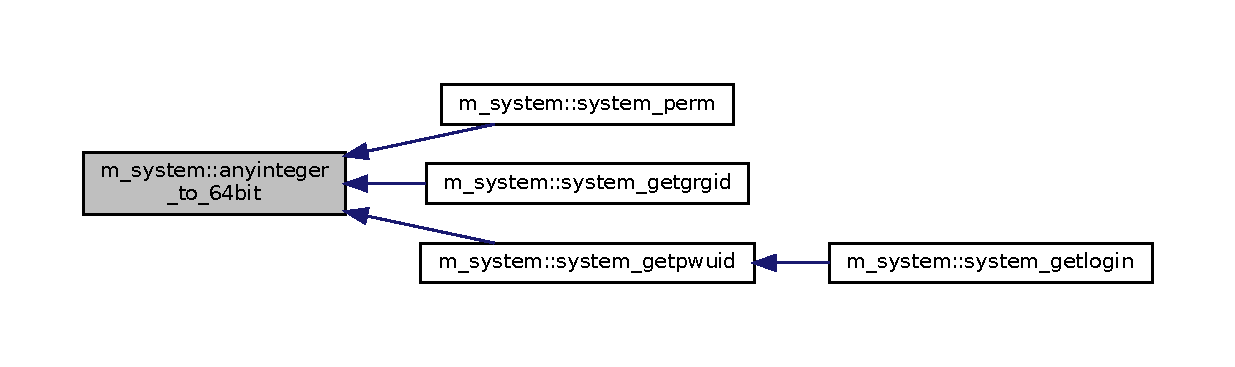
\includegraphics[width=350pt]{namespacem__system_a151da54be39dddcf270cceeff3243438_icgraph}
\end{center}
\end{figure}
\mbox{\Hypertarget{namespacem__system_aeb3d7d4cb39d59917910a3ae2532206d}\label{namespacem__system_aeb3d7d4cb39d59917910a3ae2532206d}} 
\index{m\+\_\+system@{m\+\_\+system}!arr2str@{arr2str}}
\index{arr2str@{arr2str}!m\+\_\+system@{m\+\_\+system}}
\subsubsection{\texorpdfstring{arr2str()}{arr2str()}}
{\footnotesize\ttfamily pure character(len=size(array)) function m\+\_\+system\+::arr2str (\begin{DoxyParamCaption}\item[{character(len=1), dimension(\+:), intent(in)}]{array }\end{DoxyParamCaption})\hspace{0.3cm}{\ttfamily [private]}}

Here is the caller graph for this function\+:
\nopagebreak
\begin{figure}[H]
\begin{center}
\leavevmode
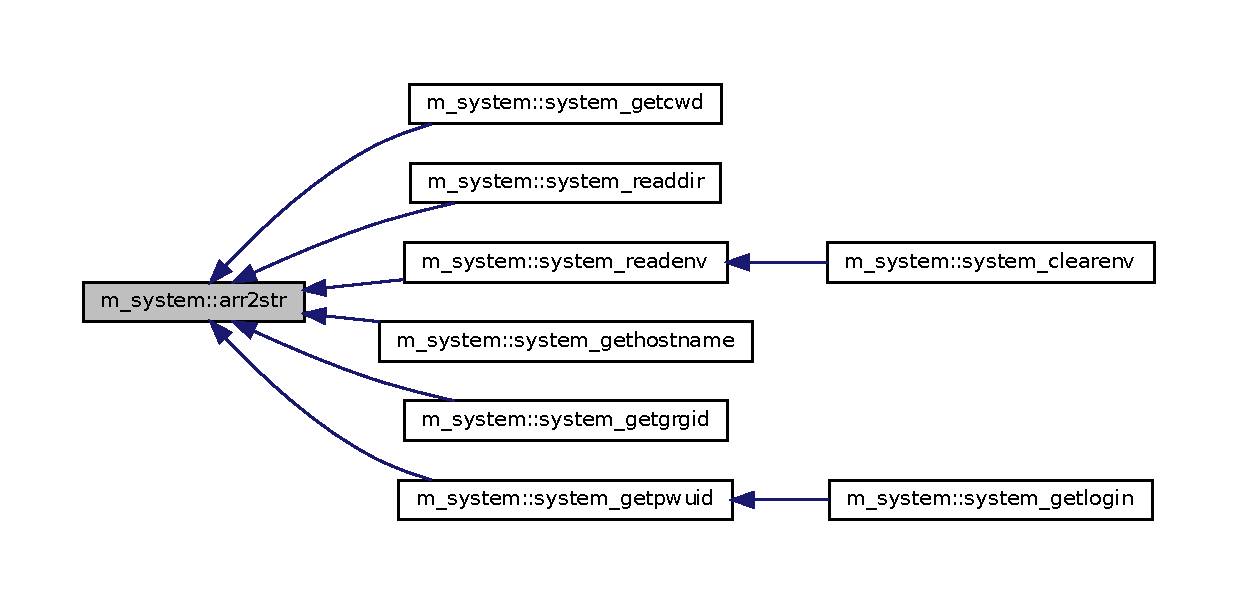
\includegraphics[width=350pt]{namespacem__system_aeb3d7d4cb39d59917910a3ae2532206d_icgraph}
\end{center}
\end{figure}
\mbox{\Hypertarget{namespacem__system_aa7c5445619aa15cd2301fe17f7c3b73c}\label{namespacem__system_aa7c5445619aa15cd2301fe17f7c3b73c}} 
\index{m\+\_\+system@{m\+\_\+system}!c2f\+\_\+string@{c2f\+\_\+string}}
\index{c2f\+\_\+string@{c2f\+\_\+string}!m\+\_\+system@{m\+\_\+system}}
\subsubsection{\texorpdfstring{c2f\+\_\+string()}{c2f\_string()}}
{\footnotesize\ttfamily character(len=\+:) function, allocatable m\+\_\+system\+::c2f\+\_\+string (\begin{DoxyParamCaption}\item[{type(c\+\_\+ptr), intent(in)}]{c\+\_\+string\+\_\+pointer }\end{DoxyParamCaption})\hspace{0.3cm}{\ttfamily [private]}}

Here is the caller graph for this function\+:
\nopagebreak
\begin{figure}[H]
\begin{center}
\leavevmode
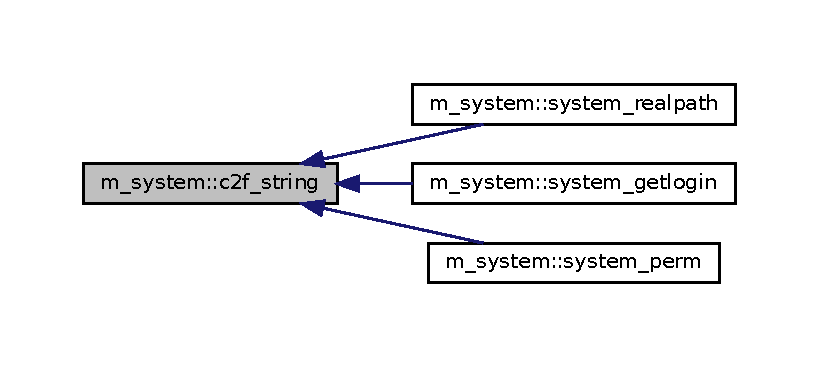
\includegraphics[width=350pt]{namespacem__system_aa7c5445619aa15cd2301fe17f7c3b73c_icgraph}
\end{center}
\end{figure}
\mbox{\Hypertarget{namespacem__system_a79656f76ad75168302e0d770052e901e}\label{namespacem__system_a79656f76ad75168302e0d770052e901e}} 
\index{m\+\_\+system@{m\+\_\+system}!fileglob@{fileglob}}
\index{fileglob@{fileglob}!m\+\_\+system@{m\+\_\+system}}
\subsubsection{\texorpdfstring{fileglob()}{fileglob()}}
{\footnotesize\ttfamily subroutine, public m\+\_\+system\+::fileglob (\begin{DoxyParamCaption}\item[{character(len=$\ast$), intent(in)}]{glob,  }\item[{character(len=$\ast$), dimension(\+:), pointer}]{list }\end{DoxyParamCaption})}



\subsubsection*{N\+A\+ME}

fileglob(3f) -\/ \mbox{[}M\+\_\+system\mbox{]} Read output of an ls(1) command from Fortran (L\+I\+C\+E\+N\+SE\+:PD) 

\subsubsection*{S\+Y\+N\+O\+P\+S\+IS}

subroutine fileglob(glob,list)

character(len=$\ast$),intent(in) \+:\+: glob character(len=$\ast$),pointer \+:\+: list(\+:)

\subsubsection*{D\+E\+S\+C\+R\+I\+P\+T\+I\+ON}

Non-\/portable procedure uses the shell and the ls(1) command to expand a filename and returns a pointer to a list of expanded filenames.

\subsubsection*{O\+P\+T\+I\+O\+NS}

glob Pattern for the filenames (like\+: $\ast$.txt) list Allocated list of filenames (returned), the caller must deallocate it.

\subsubsection*{E\+X\+A\+M\+P\+LE}

Read output of an ls(1) command from Fortran

program demo\+\_\+fileglob ! simple unit test call tryit(\textquotesingle{}$\ast$.$\ast$\textquotesingle{}) call tryit(\textquotesingle{}/tmp/\+\_\+\+\_\+notthere.txt\textquotesingle{}) contains

subroutine tryit(string) use M\+\_\+system, only \+: fileglob character(len=255),pointer \+:\+: list(\+:) character(len=$\ast$) \+:\+: string call fileglob(string, list) write($\ast$,$\ast$)\textquotesingle{}Files\+:\textquotesingle{},size(list) write($\ast$,\textquotesingle{}(a)\textquotesingle{})(trim(list(i)),i=1,size(list)) deallocate(list) end subroutine tryit

end program demo\+\_\+fileglob ! simple unit test

\subsubsection*{A\+U\+T\+H\+OR}

John S. Urban \subsubsection*{L\+I\+C\+E\+N\+SE}

Public Domain 

References uniq().

Here is the call graph for this function\+:
\nopagebreak
\begin{figure}[H]
\begin{center}
\leavevmode
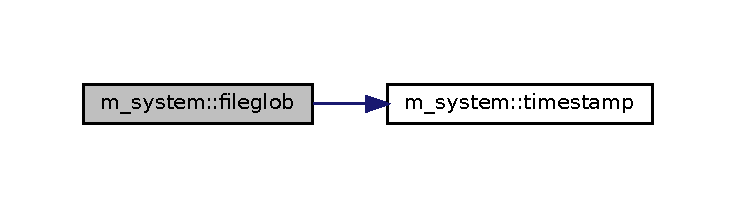
\includegraphics[width=321pt]{namespacem__system_a79656f76ad75168302e0d770052e901e_cgraph}
\end{center}
\end{figure}
\mbox{\Hypertarget{namespacem__system_ad813765403a5d9d6fb7a2edcb669fe4b}\label{namespacem__system_ad813765403a5d9d6fb7a2edcb669fe4b}} 
\index{m\+\_\+system@{m\+\_\+system}!set\+\_\+environment\+\_\+variable@{set\+\_\+environment\+\_\+variable}}
\index{set\+\_\+environment\+\_\+variable@{set\+\_\+environment\+\_\+variable}!m\+\_\+system@{m\+\_\+system}}
\subsubsection{\texorpdfstring{set\+\_\+environment\+\_\+variable()}{set\_environment\_variable()}}
{\footnotesize\ttfamily subroutine, public m\+\_\+system\+::set\+\_\+environment\+\_\+variable (\begin{DoxyParamCaption}\item[{character(len=$\ast$)}]{N\+A\+ME,  }\item[{character(len=$\ast$)}]{V\+A\+L\+UE,  }\item[{integer, intent(out), optional}]{S\+T\+A\+T\+US }\end{DoxyParamCaption})}



\subsubsection*{N\+A\+ME}

set\+\_\+environment\+\_\+variable(3f) -\/ \mbox{[}M\+\_\+system\+:E\+N\+V\+I\+R\+O\+N\+M\+E\+NT\mbox{]} call setenv(3c) to set environment variable (L\+I\+C\+E\+N\+SE\+:PD) 

\subsubsection*{S\+Y\+N\+O\+P\+S\+IS}

subroutine set\+\_\+environment\+\_\+variable(\+N\+A\+M\+E, V\+A\+L\+U\+E, S\+T\+A\+T\+U\+S)

character(len=$\ast$) \+:\+: N\+A\+ME character(len=$\ast$) \+:\+: V\+A\+L\+UE integer, optional, intent(out) \+:\+: S\+T\+A\+T\+US

\subsubsection*{D\+E\+S\+C\+R\+I\+P\+T\+I\+ON}

The \mbox{\hyperlink{namespacem__system_ad813765403a5d9d6fb7a2edcb669fe4b}{set\+\_\+environment\+\_\+variable()}} procedure adds or changes the value of environment variables.

\subsubsection*{O\+P\+T\+I\+O\+NS}

N\+A\+ME If name does not already exist in the environment, then string is added to the environment. If name does exist, then the value of name in the environment is changed to value. V\+A\+L\+UE Value to assign to environment variable N\+A\+ME S\+T\+A\+T\+US returns zero on success, or nonzero if an error occurs. A non-\/zero error usually indicates sufficient memory does not exist to store the variable.

\subsubsection*{E\+X\+A\+M\+P\+LE}

Sample setting an environment variable from Fortran\+:

program demo\+\_\+set\+\_\+environment\+\_\+variable use M\+\_\+system, only \+: set\+\_\+environment\+\_\+variable use iso\+\_\+c\+\_\+binding implicit none integer \+:\+: ierr !! write($\ast$,\textquotesingle{}(a)\textquotesingle{})\textquotesingle{}no environment variables containing \char`\"{}\+G\+R\+U\char`\"{}\+:\textquotesingle{} call execute\+\_\+command\+\_\+line(\textquotesingle{}env$\vert$grep G\+RU\textquotesingle{}) !! call set\+\_\+environment\+\_\+variable(\textquotesingle{}G\+RU\textquotesingle{},\textquotesingle{}this is the value\textquotesingle{},ierr) write($\ast$,\textquotesingle{}(a,i0)\textquotesingle{})\textquotesingle{}now \char`\"{}\+G\+R\+U\char`\"{} should be defined, status=\textquotesingle{},ierr call execute\+\_\+command\+\_\+line(\textquotesingle{}env$\vert$grep G\+RU\textquotesingle{}) !! call set\+\_\+environment\+\_\+variable(\textquotesingle{}G\+R\+U2\textquotesingle{},\textquotesingle{}this is the second value\textquotesingle{},ierr) write($\ast$,\textquotesingle{}(a,i0)\textquotesingle{})\textquotesingle{}now \char`\"{}\+G\+R\+U\char`\"{} and \char`\"{}\+G\+R\+U2\char`\"{} should be defined, status =\textquotesingle{},ierr !! call execute\+\_\+command\+\_\+line(\textquotesingle{}env$\vert$grep G\+RU\textquotesingle{}) end program demo\+\_\+set\+\_\+environment\+\_\+variable

Results\+:

no environment variables containing \char`\"{}\+G\+R\+U\char`\"{}\+: now \char`\"{}\+G\+R\+U\char`\"{} should be defined, status=0 G\+RU=this is the value now \char`\"{}\+G\+R\+U\char`\"{} and \char`\"{}\+G\+R\+U2\char`\"{} should be defined, status =0 G\+R\+U2=this is the second value G\+RU=this is the value \subsubsection*{A\+U\+T\+H\+OR}

John S. Urban \subsubsection*{L\+I\+C\+E\+N\+SE}

Public Domain 

References str2arr().

Here is the call graph for this function\+:
\nopagebreak
\begin{figure}[H]
\begin{center}
\leavevmode
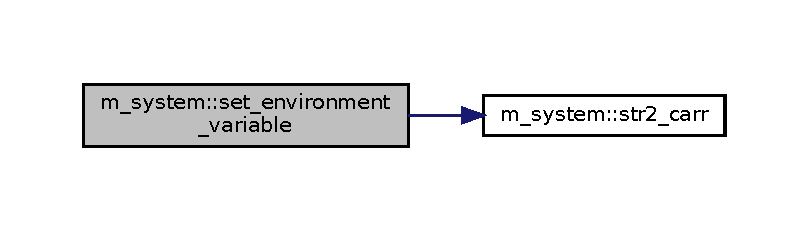
\includegraphics[width=350pt]{namespacem__system_ad813765403a5d9d6fb7a2edcb669fe4b_cgraph}
\end{center}
\end{figure}
\mbox{\Hypertarget{namespacem__system_af7e778ffc24aa7bc00b842a8e673aeaa}\label{namespacem__system_af7e778ffc24aa7bc00b842a8e673aeaa}} 
\index{m\+\_\+system@{m\+\_\+system}!str2arr@{str2arr}}
\index{str2arr@{str2arr}!m\+\_\+system@{m\+\_\+system}}
\subsubsection{\texorpdfstring{str2arr()}{str2arr()}}
{\footnotesize\ttfamily pure character(len=1,kind=c\+\_\+char) function, dimension(len(string)+1) m\+\_\+system\+::str2arr (\begin{DoxyParamCaption}\item[{character(len=$\ast$), intent(in)}]{string }\end{DoxyParamCaption})\hspace{0.3cm}{\ttfamily [private]}}

Here is the caller graph for this function\+:
\nopagebreak
\begin{figure}[H]
\begin{center}
\leavevmode
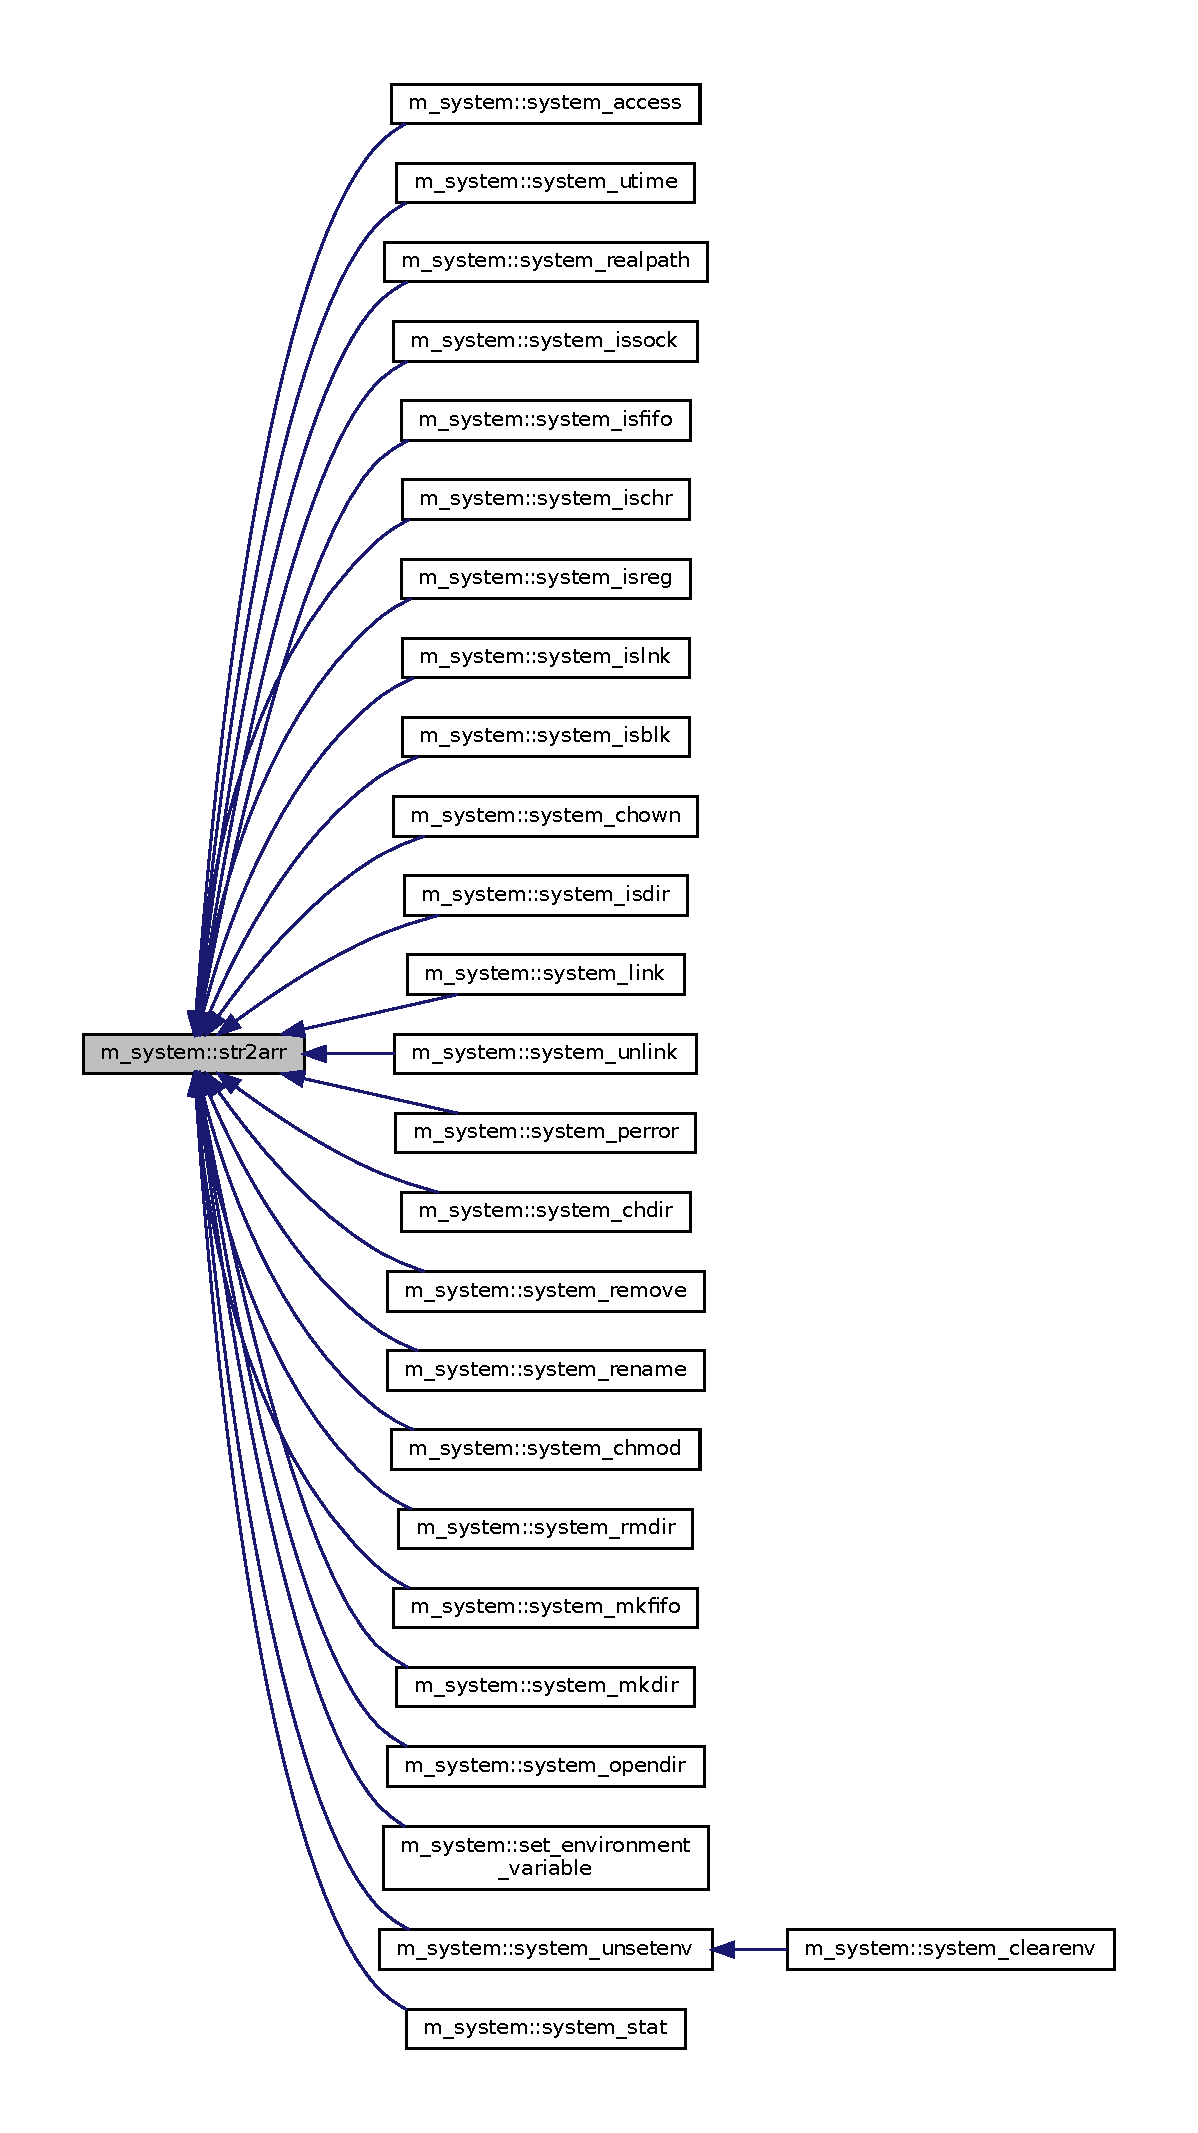
\includegraphics[height=550pt]{namespacem__system_af7e778ffc24aa7bc00b842a8e673aeaa_icgraph}
\end{center}
\end{figure}
\mbox{\Hypertarget{namespacem__system_a4687a363acbb7084a51bc77844789275}\label{namespacem__system_a4687a363acbb7084a51bc77844789275}} 
\index{m\+\_\+system@{m\+\_\+system}!system\+\_\+access@{system\+\_\+access}}
\index{system\+\_\+access@{system\+\_\+access}!m\+\_\+system@{m\+\_\+system}}
\subsubsection{\texorpdfstring{system\+\_\+access()}{system\_access()}}
{\footnotesize\ttfamily logical function, public m\+\_\+system\+::system\+\_\+access (\begin{DoxyParamCaption}\item[{character(len=$\ast$), intent(in)}]{pathname,  }\item[{integer, intent(in)}]{amode }\end{DoxyParamCaption})}



\subsubsection*{N\+A\+ME}

system\+\_\+access(3f) -\/ \mbox{[}M\+\_\+system\mbox{]} checks accessibility or existence of a pathname (L\+I\+C\+E\+N\+SE\+:PD) 

\subsubsection*{S\+Y\+N\+O\+P\+S\+IS}

logical function system\+\_\+access(pathname,amode)

character(len=$\ast$),intent(in) \+:\+: pathname integer,intent(in) \+:\+: amode

\subsubsection*{D\+E\+S\+C\+R\+I\+P\+T\+I\+ON}

\begin{DoxyVerb}The system_access(3f) function checks pathname existence and access
permissions. The function checks the pathname for accessibility
according to the bit pattern contained in amode, using the real user
ID in place of the effective user ID and the real group ID in place
of the effective group ID.

The value of amode is either the bitwise-inclusive OR of the access
permissions to be checked (R_OK, W_OK, X_OK) or the existence test (F_OK).
\end{DoxyVerb}


\subsubsection*{O\+P\+T\+I\+O\+NS}

pathname a character string representing a directory pathname. Trailing spaces are ignored. amode bitwise-\/inclusive OR of the values R\+\_\+\+OK, W\+\_\+\+OK, X\+\_\+\+OK, or F\+\_\+\+OK.

\subsubsection*{R\+E\+T\+U\+RN V\+A\+L\+UE}

If not true an error occurred or the requested access is not granted

\subsubsection*{E\+X\+A\+M\+P\+LE}

check if filename is accessible \begin{DoxyVerb} Sample program:

    program demo_system_access
    Use M_system, only : system_access, F_OK, R_OK, W_OK, X_OK
    implicit none
    integer                     :: i
    character(len=80),parameter :: names(*)=[ &
    '/usr/bin/bash   ', &
    '/tmp/NOTTHERE   ', &
    '/usr/local      ', &
    '.               ', &
    'PROBABLY_NOT    ']
    do i=1,size(names)
       write(*,*)' does ',trim(names(i)),' exist?    ', system_access(names(i),F_OK)
       write(*,*)' is ',trim(names(i)),' readable?     ', system_access(names(i),R_OK)
       write(*,*)' is ',trim(names(i)),' writeable?    ', system_access(names(i),W_OK)
       write(*,*)' is ',trim(names(i)),' executable?   ', system_access(names(i),X_OK)
    enddo
    end program demo_system_access \end{DoxyVerb}
 

References str2arr().

Here is the call graph for this function\+:
\nopagebreak
\begin{figure}[H]
\begin{center}
\leavevmode
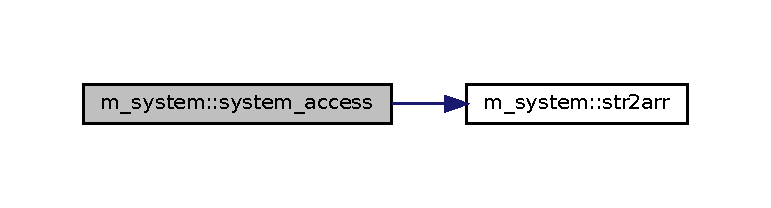
\includegraphics[width=350pt]{namespacem__system_a4687a363acbb7084a51bc77844789275_cgraph}
\end{center}
\end{figure}
\mbox{\Hypertarget{namespacem__system_a47746b670cb21bae0957c9bb2bccf209}\label{namespacem__system_a47746b670cb21bae0957c9bb2bccf209}} 
\index{m\+\_\+system@{m\+\_\+system}!system\+\_\+chdir@{system\+\_\+chdir}}
\index{system\+\_\+chdir@{system\+\_\+chdir}!m\+\_\+system@{m\+\_\+system}}
\subsubsection{\texorpdfstring{system\+\_\+chdir()}{system\_chdir()}}
{\footnotesize\ttfamily subroutine, public m\+\_\+system\+::system\+\_\+chdir (\begin{DoxyParamCaption}\item[{character(len=$\ast$)}]{path,  }\item[{integer, intent(out), optional}]{err }\end{DoxyParamCaption})}



\subsubsection*{N\+A\+ME}

system\+\_\+chdir(3f) -\/ \mbox{[}M\+\_\+system\mbox{]} call chdir(3c) from Fortran to change working directory (L\+I\+C\+E\+N\+SE\+:PD) \subsubsection*{S\+Y\+N\+O\+P\+S\+IS}

subroutine system\+\_\+chdir(path, err)

character(len=$\ast$) \+:\+: path integer, optional, intent(out) \+:\+: err

\subsubsection*{D\+E\+S\+C\+R\+I\+P\+T\+I\+ON}

\begin{DoxyVerb}system_chdir(3f) changes the current working directory of the calling
process to the directory specified in path. The current working
directory is the starting point for interpreting relative pathnames
(those not starting with '/').
\end{DoxyVerb}


\subsubsection*{R\+E\+T\+U\+RN V\+A\+L\+UE}

\begin{DoxyVerb}On success, zero is returned. On error, -1 is returned, and errno is
set appropriately.


Depending on the file system, other errors can be returned. The more
general errors for chdir() are listed below, by their C definitions:

Errors
EACCES        Search permission is denied for one of the components of path.
              (See also path_resolution(7).)
EFAULT        path points outside your accessible address space.
EIO           An I/O error occurred.
ELOOP         Too many symbolic links were encountered in resolving path.
ENAMETOOLONG  path is too long.
ENOENT        The file does not exist.
ENOMEM        Insufficient kernel memory was available.
ENOTDIR       A component of path is not a directory.
\end{DoxyVerb}


\subsubsection*{S\+EE A\+L\+SO}

\begin{DoxyVerb}chroot(2), getcwd(3), path_resolution(7)
\end{DoxyVerb}


\subsubsection*{E\+X\+A\+M\+P\+LE}

\begin{DoxyVerb}Change working directory from Fortran

  program demo_system_chdir
  use M_system, only : system_chdir
  implicit none
  integer :: ierr

  call execute_command_line('pwd')
  call system_chdir('/tmp',ierr)
  call execute_command_line('pwd')
  write(*,*)'*CHDIR TEST* IERR=',ierr

  end program demo_system_chdir
\end{DoxyVerb}


\subsubsection*{R\+E\+S\+U\+L\+TS\+:}

Sample run output\+:

/home/urbanjs/\+V600 /tmp {\itshape C\+H\+D\+IR T\+E\+ST} I\+E\+RR= 0 

References str2arr().

Here is the call graph for this function\+:
\nopagebreak
\begin{figure}[H]
\begin{center}
\leavevmode
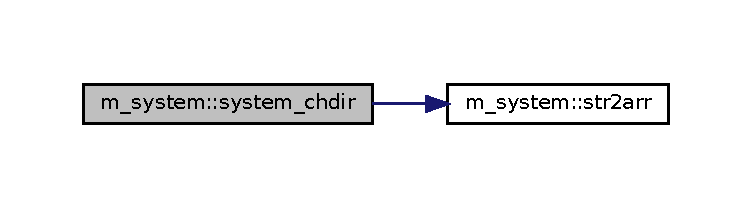
\includegraphics[width=350pt]{namespacem__system_a47746b670cb21bae0957c9bb2bccf209_cgraph}
\end{center}
\end{figure}
\mbox{\Hypertarget{namespacem__system_ace9ce0c8a9c8341a76b8903cd2390ce3}\label{namespacem__system_ace9ce0c8a9c8341a76b8903cd2390ce3}} 
\index{m\+\_\+system@{m\+\_\+system}!system\+\_\+chmod@{system\+\_\+chmod}}
\index{system\+\_\+chmod@{system\+\_\+chmod}!m\+\_\+system@{m\+\_\+system}}
\subsubsection{\texorpdfstring{system\+\_\+chmod()}{system\_chmod()}}
{\footnotesize\ttfamily integer function, public m\+\_\+system\+::system\+\_\+chmod (\begin{DoxyParamCaption}\item[{character(len=$\ast$), intent(in)}]{filename,  }\item[{integer, intent(in), value}]{mode }\end{DoxyParamCaption})}



\subsubsection*{N\+A\+ME}

system\+\_\+chmod(3f) -\/ \mbox{[}M\+\_\+system\mbox{]} call chmod(3c) to change permission mode of a file relative to directory file descriptor (L\+I\+C\+E\+N\+SE\+:PD) \subsubsection*{S\+Y\+N\+O\+P\+S\+IS}

function system\+\_\+chmod(filename,mode) result(ierr)

character(len=$\ast$),intent(in) \+:\+: filename integer,value,intent(in) \+:\+: mode integer \+:\+: ierr

\subsubsection*{D\+E\+S\+C\+R\+I\+P\+T\+I\+ON}

The system\+\_\+chmod(3f) function shall change U\+ID, \+\_\+\+I\+S\+G\+ID, S\+\_\+\+I\+S\+V\+TX, and the file permission bits of the file named by the pathname pointed to by the path argument to the corresponding bits in the mode argument. The application shall ensure that the effective user ID of the process matches the owner of the file or the process has appropriate privileges in order to do this.

S\+\_\+\+I\+S\+U\+ID, S\+\_\+\+I\+S\+G\+ID, S\+\_\+\+I\+S\+V\+TX, and the file permission bits are described in $<$sys/stat.\+h$>$.

If the calling process does not have appropriate privileges, and if the group ID of the file does not match the effective group ID or one of the supplementary group I\+Ds and if the file is a regular file, bit S\+\_\+\+I\+S\+G\+ID (set-\/group-\/\+ID on execution) in the file\textquotesingle{}s mode shall be cleared upon successful return from chmod().

Additional implementation-\/defined restrictions may cause the S\+\_\+\+I\+S\+U\+ID and S\+\_\+\+I\+S\+G\+ID bits in mode to be ignored.

Upon successful completion, \mbox{\hyperlink{namespacem__system_ace9ce0c8a9c8341a76b8903cd2390ce3}{system\+\_\+chmod()}} marks for update the last file status change timestamp of the file.

Values for flag are constructed by a bitwise-\/inclusive OR of flags from the following list, defined in $<$fcntl.\+h$>$\+:

A\+T\+\_\+\+S\+Y\+M\+L\+I\+N\+K\+\_\+\+N\+O\+F\+O\+L\+L\+OW If path names a symbolic link, then the mode of the symbolic link is changed.

\subsubsection*{R\+E\+T\+U\+RN V\+A\+L\+UE}

Upon successful completion, system\+\_\+chmod(3f) returns 0. Otherwise, it returns -\/1 and sets errno to indicate the error. If -\/1 is returned, no change to the file mode occurs.

\subsubsection*{E\+X\+A\+M\+P\+L\+ES}

Sample program\+:

program demo\+\_\+system\+\_\+chmod use M\+\_\+system, only \+: system\+\_\+chmod use M\+\_\+system, only \+: system\+\_\+stat use M\+\_\+system, only \+: R\+\_\+\+G\+RP,R\+\_\+\+O\+TH,R\+\_\+\+U\+SR,R\+W\+X\+\_\+G,R\+W\+X\+\_\+O use M\+\_\+system, only \+: R\+W\+X\+\_\+U,W\+\_\+\+G\+RP,W\+\_\+\+O\+TH,W\+\_\+\+U\+SR,X\+\_\+\+G\+RP,X\+\_\+\+O\+TH,X\+\_\+\+U\+SR use M\+\_\+system, only \+: D\+E\+F\+F\+I\+L\+E\+M\+O\+DE, A\+C\+C\+E\+S\+S\+P\+E\+R\+MS use,intrinsic \+:\+: iso\+\_\+fortran\+\_\+env, only \+: int64 implicit none integer \+:\+: ierr integer \+:\+: status integer(kind=int64) \+:\+: buffer(13) !\+Setting Read Permissions for User, Group, and Others ! The following example sets read permissions for the owner, group, and others. open(file=\textquotesingle{}\+\_\+test1\textquotesingle{},unit=10) write(10,$\ast$)\textquotesingle{}T\+E\+ST F\+I\+LE 1\textquotesingle{} close(unit=10) ierr=system\+\_\+chmod(\textquotesingle{}\+\_\+test1\textquotesingle{}, I\+A\+N\+Y(\mbox{[}\+R\+\_\+\+U\+S\+R,\+R\+\_\+\+G\+R\+P,\+R\+\_\+\+O\+T\+H\mbox{]}))

!\+Setting Read, Write, and Execute Permissions for the Owner Only ! The following example sets read, write, and execute permissions for the owner, and no permissions for group and others. open(file=\textquotesingle{}\+\_\+test2\textquotesingle{},unit=10) write(10,$\ast$)\textquotesingle{}T\+E\+ST F\+I\+LE 2\textquotesingle{} close(unit=10) ierr=system\+\_\+chmod(\textquotesingle{}\+\_\+test2\textquotesingle{}, R\+W\+X\+\_\+U)

!\+Setting Different Permissions for Owner, Group, and Other ! The following example sets owner permissions for C\+H\+A\+N\+G\+E\+F\+I\+LE to read, write, and execute, group permissions to read and ! execute, and other permissions to read. open(file=\textquotesingle{}\+\_\+test3\textquotesingle{},unit=10) write(10,$\ast$)\textquotesingle{}T\+E\+ST F\+I\+LE 3\textquotesingle{} close(unit=10) ierr=system\+\_\+chmod(\textquotesingle{}\+\_\+test3\textquotesingle{}, I\+A\+N\+Y(\mbox{[}\+R\+W\+X\+\_\+\+U,\+R\+\_\+\+G\+R\+P,\+X\+\_\+\+G\+R\+P,\+R\+\_\+\+O\+T\+H\mbox{]}));

!\+Setting and Checking File Permissions ! The following example sets the file permission bits for a file named /home/cnd/mod1, then calls the stat() function to ! verify the permissions.

ierr=system\+\_\+chmod(\char`\"{}home/cnd/mod1\char`\"{}, I\+A\+N\+Y(\mbox{[}\+R\+W\+X\+\_\+\+U,\+R\+W\+X\+\_\+\+G,\+R\+\_\+\+O\+T\+H,\+W\+\_\+\+O\+T\+H\mbox{]})) call system\+\_\+stat(\char`\"{}home/cnd/mod1\char`\"{}, buffer,status)

! In order to ensure that the S\+\_\+\+I\+S\+U\+ID and S\+\_\+\+I\+S\+G\+ID bits are set, an application requiring this should use stat() after a ! successful chmod() to verify this.

! Any files currently open could possibly become invalid if the mode ! of the file is changed to a value which would deny access to ! that process.

end program demo\+\_\+system\+\_\+chmod

\subsubsection*{A\+U\+T\+H\+OR}

John S. Urban \subsubsection*{L\+I\+C\+E\+N\+SE}

Public Domain 

References str2arr().

Here is the call graph for this function\+:
\nopagebreak
\begin{figure}[H]
\begin{center}
\leavevmode
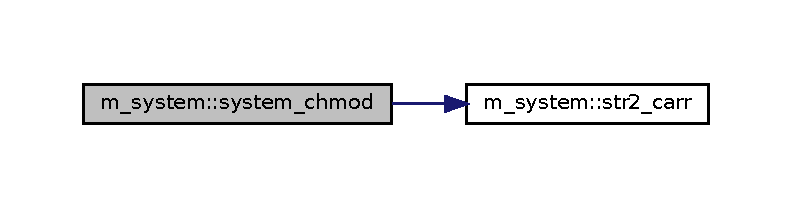
\includegraphics[width=350pt]{namespacem__system_ace9ce0c8a9c8341a76b8903cd2390ce3_cgraph}
\end{center}
\end{figure}
\mbox{\Hypertarget{namespacem__system_a3353c1cff032fcfe2985a69f10038ddd}\label{namespacem__system_a3353c1cff032fcfe2985a69f10038ddd}} 
\index{m\+\_\+system@{m\+\_\+system}!system\+\_\+chown@{system\+\_\+chown}}
\index{system\+\_\+chown@{system\+\_\+chown}!m\+\_\+system@{m\+\_\+system}}
\subsubsection{\texorpdfstring{system\+\_\+chown()}{system\_chown()}}
{\footnotesize\ttfamily logical function, public m\+\_\+system\+::system\+\_\+chown (\begin{DoxyParamCaption}\item[{character(len=$\ast$), intent(in)}]{dirname,  }\item[{integer, intent(in)}]{owner,  }\item[{integer, intent(in)}]{group }\end{DoxyParamCaption})}



\subsubsection*{N\+A\+ME}

system\+\_\+chown(3f) -\/ \mbox{[}M\+\_\+system\mbox{]} change file owner and group (L\+I\+C\+E\+N\+SE\+:PD) 

\subsubsection*{S\+Y\+N\+O\+P\+S\+IS}

logical function system\+\_\+chown(path,owner,group)

character(len=$\ast$),intent(in) \+:\+: path integer,intent(in) \+:\+: owner integer,intent(in) \+:\+: group

\subsubsection*{D\+E\+S\+C\+R\+I\+P\+T\+I\+ON}

The chown(3f) function changes owner and group of a file

The path argument points to a pathname naming a file. The user ID and group ID of the named file shall be set to the numeric values contained in owner and group, respectively.

Only processes with an effective user ID equal to the user ID of the file or with appropriate privileges may change the ownership of a file.

\subsubsection*{O\+P\+T\+I\+O\+NS}

path a character string representing a file pathname. Trailing spaces are ignored. owner U\+ID of owner that ownership is to be changed to group G\+ID of group that ownership is to be changed to

\subsubsection*{R\+E\+T\+U\+RN V\+A\+L\+UE}

The \mbox{\hyperlink{namespacem__system_a3353c1cff032fcfe2985a69f10038ddd}{system\+\_\+chown()}} function should return zero (0) if successful. Otherwise, these functions shall return 1 and set errno to indicate the error. If 1 is returned, no changes are made in the user ID and group ID of the file.

\subsubsection*{E\+X\+A\+M\+P\+LE}

Sample program\+:

program demo\+\_\+system\+\_\+chown Use M\+\_\+system, only \+: system\+\_\+chown Use M\+\_\+system, only \+: \mbox{\hyperlink{interfacem__system_1_1system__getuid}{system\+\_\+getuid}} Use M\+\_\+system, only \+: \mbox{\hyperlink{interfacem__system_1_1system__getgid}{system\+\_\+getgid}} use M\+\_\+system, only \+: system\+\_\+perror implicit none integer \+:\+: i character(len=80),parameter \+:\+: names($\ast$)=\mbox{[}character(len=80) \+:\+: \textquotesingle{}myfile1\textquotesingle{},\textquotesingle{}/usr/local\textquotesingle{}\mbox{]} do i=1,size(names) if(.not. system\+\_\+chown(\& \& trim(names(i)), \& \& system\+\_\+getuid(), \& \& system\+\_\+getgid()) \& )then call system\+\_\+perror(\textquotesingle{}{\itshape demo\+\_\+system\+\_\+chown} \textquotesingle{}//trim(names(i))) endif enddo end program demo\+\_\+system\+\_\+chown 

References str2arr().

Here is the call graph for this function\+:
\nopagebreak
\begin{figure}[H]
\begin{center}
\leavevmode
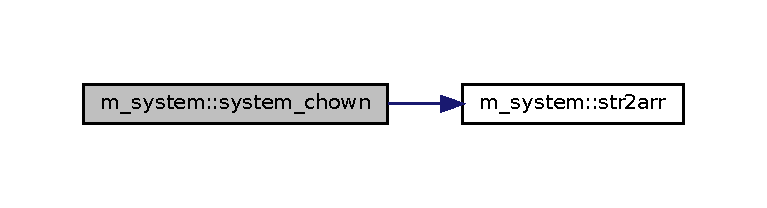
\includegraphics[width=350pt]{namespacem__system_a3353c1cff032fcfe2985a69f10038ddd_cgraph}
\end{center}
\end{figure}
\mbox{\Hypertarget{namespacem__system_a9c34787b170ab8d41000d7c3acb60736}\label{namespacem__system_a9c34787b170ab8d41000d7c3acb60736}} 
\index{m\+\_\+system@{m\+\_\+system}!system\+\_\+clearenv@{system\+\_\+clearenv}}
\index{system\+\_\+clearenv@{system\+\_\+clearenv}!m\+\_\+system@{m\+\_\+system}}
\subsubsection{\texorpdfstring{system\+\_\+clearenv()}{system\_clearenv()}}
{\footnotesize\ttfamily subroutine, public m\+\_\+system\+::system\+\_\+clearenv (\begin{DoxyParamCaption}\item[{integer, intent(out), optional}]{ierr }\end{DoxyParamCaption})}



\subsubsection*{N\+A\+ME}

system\+\_\+clearenv(3f) -\/ \mbox{[}M\+\_\+system\+:E\+N\+V\+I\+R\+O\+N\+M\+E\+NT\mbox{]} clear environment by calling clearenv(3c) (L\+I\+C\+E\+N\+SE\+:PD) 

\subsubsection*{S\+Y\+N\+O\+P\+S\+IS}

\begin{DoxyVerb}subroutine system_clearenv(ierr)

 integer,intent(out),optional :: ierr
\end{DoxyVerb}


\subsubsection*{D\+E\+S\+C\+R\+I\+P\+T\+I\+ON}

The clearenv() procedure clears the environment of all name-\/value pairs. Typically used in security-\/conscious applications or ones where configuration control requires ensuring specific variables are set.

\subsubsection*{R\+E\+T\+U\+RN V\+A\+L\+U\+ES}

ierr returns zero on success, and a nonzero value on failure. Optional. If not present and an error occurs the program stops.

\subsubsection*{E\+X\+A\+M\+P\+LE}

Sample program\+:

program demo\+\_\+system\+\_\+clearenv use M\+\_\+system, only \+: system\+\_\+clearenv implicit none ! environment before clearing call execute\+\_\+command\+\_\+line(\textquotesingle{}env$\vert$wc\textquotesingle{}) ! environment after clearing (not necessarily blank!!) call \mbox{\hyperlink{namespacem__system_a9c34787b170ab8d41000d7c3acb60736}{system\+\_\+clearenv()}} call execute\+\_\+command\+\_\+line(\textquotesingle{}env\textquotesingle{}) end program demo\+\_\+system\+\_\+clearenv

Typical output\+:

89 153 7427 P\+WD=/home/urbanjs/\+V600 S\+H\+L\+VL=1

\subsubsection*{A\+U\+T\+H\+OR}

John S. Urban \subsubsection*{L\+I\+C\+E\+N\+SE}

Public Domain 

References system\+\_\+readenv(), and system\+\_\+unsetenv().

Here is the call graph for this function\+:
\nopagebreak
\begin{figure}[H]
\begin{center}
\leavevmode
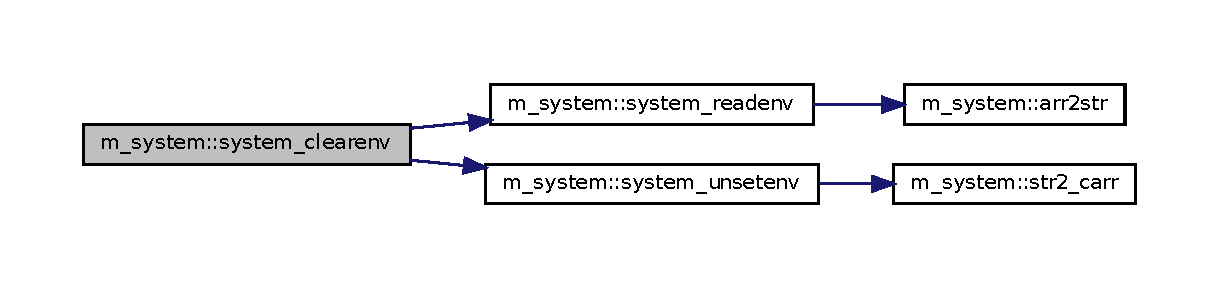
\includegraphics[width=350pt]{namespacem__system_a9c34787b170ab8d41000d7c3acb60736_cgraph}
\end{center}
\end{figure}
\mbox{\Hypertarget{namespacem__system_acd442b52c64fc50482bc08b0ac8a50d1}\label{namespacem__system_acd442b52c64fc50482bc08b0ac8a50d1}} 
\index{m\+\_\+system@{m\+\_\+system}!system\+\_\+closedir@{system\+\_\+closedir}}
\index{system\+\_\+closedir@{system\+\_\+closedir}!m\+\_\+system@{m\+\_\+system}}
\subsubsection{\texorpdfstring{system\+\_\+closedir()}{system\_closedir()}}
{\footnotesize\ttfamily subroutine, public m\+\_\+system\+::system\+\_\+closedir (\begin{DoxyParamCaption}\item[{type(c\+\_\+ptr), value}]{dir,  }\item[{integer, intent(out), optional}]{ierr }\end{DoxyParamCaption})}



\subsubsection*{N\+A\+ME}

system\+\_\+closedir(3f) -\/ \mbox{[}M\+\_\+system\mbox{]} close a directory stream by calling closedir(3c) (L\+I\+C\+E\+N\+SE\+:PD) \subsubsection*{S\+Y\+N\+O\+P\+S\+IS}

subroutine system\+\_\+closedir(dir,ierr)

type(c\+\_\+ptr) \+:\+: dir integer,intent(out) \+:\+: ierr \subsubsection*{D\+E\+S\+C\+R\+I\+P\+T\+I\+ON}

The S\+Y\+S\+T\+E\+M\+\_\+\+C\+L\+O\+S\+E\+D\+I\+R(3f) function closes the directory stream referred to by the argument D\+IR. Upon return, the value of D\+IR may no longer point to an accessible object. \subsubsection*{O\+P\+T\+I\+O\+NS}

dir directory stream pointer opened by S\+Y\+S\+T\+E\+M\+\_\+\+O\+P\+E\+N\+D\+I\+R(3f). ierr Upon successful completion, S\+Y\+S\+T\+E\+M\+\_\+\+C\+L\+O\+S\+E\+D\+I\+R(3f) returns 0; otherwise, an error has occurred. \subsubsection*{E\+R\+R\+O\+RS}

system\+\_\+closedir(3f) may fail if\+:

E\+B\+A\+DF The dirp argument does not refer to an open directory stream. E\+I\+N\+TR The closedir() function was interrupted by a signal. \subsubsection*{E\+X\+A\+M\+P\+LE}

Sample program

program demo\+\_\+system\+\_\+closedir use M\+\_\+system, only \+: system\+\_\+opendir,system\+\_\+readdir use M\+\_\+system, only \+: system\+\_\+closedir, system\+\_\+rewinddir use iso\+\_\+c\+\_\+binding, only \+: c\+\_\+ptr implicit none type(c\+\_\+ptr) \+:\+: dir character(len=\+:),allocatable \+:\+: filename integer \+:\+: ierr !--- open directory stream to read from call system\+\_\+opendir(\textquotesingle{}.\textquotesingle{},dir,ierr) !--- read directory stream do call system\+\_\+readdir(dir,filename,ierr) if(filename.\+eq.\textquotesingle{} \textquotesingle{})exit write($\ast$,$\ast$)filename enddo call system\+\_\+rewinddir(dir) !--- close directory stream call system\+\_\+closedir(dir,ierr) end program demo\+\_\+system\+\_\+closedir \subsubsection*{A\+U\+T\+H\+OR}

John S. Urban \subsubsection*{L\+I\+C\+E\+N\+SE}

Public Domain \mbox{\Hypertarget{namespacem__system_a257d2b8987db850bc686507f19ccbe4a}\label{namespacem__system_a257d2b8987db850bc686507f19ccbe4a}} 
\index{m\+\_\+system@{m\+\_\+system}!system\+\_\+cpu\+\_\+time@{system\+\_\+cpu\+\_\+time}}
\index{system\+\_\+cpu\+\_\+time@{system\+\_\+cpu\+\_\+time}!m\+\_\+system@{m\+\_\+system}}
\subsubsection{\texorpdfstring{system\+\_\+cpu\+\_\+time()}{system\_cpu\_time()}}
{\footnotesize\ttfamily subroutine, public m\+\_\+system\+::system\+\_\+cpu\+\_\+time (\begin{DoxyParamCaption}\item[{real, intent(out)}]{total,  }\item[{real, intent(out)}]{user,  }\item[{real, intent(out)}]{system }\end{DoxyParamCaption})}



\subsubsection*{N\+A\+ME}

system\+\_\+cpu\+\_\+time(3f) -\/ \mbox{[}M\+\_\+system\mbox{]} get processor time by calling times(3c) (L\+I\+C\+E\+N\+SE\+:PD) 

\subsubsection*{S\+Y\+N\+O\+P\+S\+IS}

\begin{DoxyVerb}    subroutine system_cpu_time(c_user, c_system, c_total)

     real,intent(out) :: c_total
     real,intent(out) :: c_user
     real,intent(out) :: c_system
\end{DoxyVerb}


\subsubsection*{D\+E\+S\+C\+R\+I\+P\+T\+I\+ON}

\subsubsection*{O\+U\+T\+P\+UT}

c\+\_\+total total processor time ( c\+\_\+user + c\+\_\+system ) c\+\_\+user processor user time c\+\_\+system processor system time

\subsubsection*{E\+R\+R\+O\+RS}

No errors are defined.

\subsubsection*{E\+X\+A\+M\+P\+L\+ES}

Sample program\+:

program demo\+\_\+system\+\_\+cpu\+\_\+time

use M\+\_\+system, only \+: system\+\_\+cpu\+\_\+time use I\+S\+O\+\_\+\+C\+\_\+\+B\+I\+N\+D\+I\+NG, only \+: c\+\_\+float implicit none real \+:\+: user\+\_\+start, system\+\_\+start, total\+\_\+start real \+:\+: user\+\_\+finish, system\+\_\+finish, total\+\_\+finish integer \+:\+: i integer \+:\+: itimes=1000000 real \+:\+: value

call system\+\_\+cpu\+\_\+time(total\+\_\+start,user\+\_\+start,system\+\_\+start)

value=0.\+0 do i=1,itimes value=sqrt(real(i)+value) enddo write(10,$\ast$)value flush(10) write($\ast$,$\ast$)\textquotesingle{}average sqrt value=\textquotesingle{},value/itimes call system\+\_\+cpu\+\_\+time(total\+\_\+finish,user\+\_\+finish,system\+\_\+finish) write($\ast$,$\ast$)\textquotesingle{}U\+S\+ER ......\textquotesingle{},user\+\_\+finish-\/user\+\_\+start write($\ast$,$\ast$)\textquotesingle{}S\+Y\+S\+T\+EM ....\textquotesingle{},system\+\_\+finish-\/system\+\_\+start write($\ast$,$\ast$)\textquotesingle{}T\+O\+T\+AL .....\textquotesingle{},total\+\_\+finish-\/total\+\_\+start

end program demo\+\_\+system\+\_\+cpu\+\_\+time

Typical Results\+: \mbox{\Hypertarget{namespacem__system_a5a32db818a9ffb0a4ea724e95356c560}\label{namespacem__system_a5a32db818a9ffb0a4ea724e95356c560}} 
\index{m\+\_\+system@{m\+\_\+system}!system\+\_\+getcwd@{system\+\_\+getcwd}}
\index{system\+\_\+getcwd@{system\+\_\+getcwd}!m\+\_\+system@{m\+\_\+system}}
\subsubsection{\texorpdfstring{system\+\_\+getcwd()}{system\_getcwd()}}
{\footnotesize\ttfamily subroutine, public m\+\_\+system\+::system\+\_\+getcwd (\begin{DoxyParamCaption}\item[{character(len=\+:), intent(out), allocatable}]{output,  }\item[{integer, intent(out)}]{ierr }\end{DoxyParamCaption})}



\subsubsection*{N\+A\+ME}

system\+\_\+getcwd(3f) -\/ \mbox{[}M\+\_\+system\mbox{]} call getcwd(3c) to get the pathname of the current working directory (L\+I\+C\+E\+N\+SE\+:PD) \subsubsection*{S\+Y\+N\+O\+P\+S\+IS}

subroutine system\+\_\+getcwd(output,ierr)

character(len=\+:),allocatable,intent(out) \+:\+: output integer,intent(out) \+:\+: ierr \subsubsection*{D\+E\+S\+C\+R\+I\+P\+T\+I\+ON}

system\+\_\+getcwd(3f) calls the C routine getcwd(3c) to obtain the absolute pathname of the current working directory.

\subsubsection*{R\+E\+T\+U\+RN V\+A\+L\+UE}

O\+U\+T\+P\+UT The absolute pathname of the current working directory The pathname shall contain no components that are dot or dot-\/dot, or are symbolic links. I\+E\+RR is not zero if an error occurs.

\subsubsection*{E\+X\+A\+M\+P\+LE}

Sample program\+:

program demo\+\_\+system\+\_\+getcwd use M\+\_\+system, only \+: system\+\_\+getcwd implicit none character(len=\+:),allocatable \+:\+: dirname integer \+:\+: ierr call system\+\_\+getcwd(dirname,ierr) if(ierr.\+eq.\+0)then write($\ast$,$\ast$)\textquotesingle{}C\+U\+R\+R\+E\+NT D\+I\+R\+E\+C\+T\+O\+RY \textquotesingle{},trim(dirname) else write($\ast$,$\ast$)\textquotesingle{}E\+R\+R\+OR O\+B\+T\+A\+I\+N\+I\+NG C\+U\+R\+R\+E\+NT D\+I\+R\+E\+C\+T\+O\+RY N\+A\+ME\textquotesingle{} endif end program demo\+\_\+system\+\_\+getcwd

\subsubsection*{A\+U\+T\+H\+OR}

John S. Urban \subsubsection*{L\+I\+C\+E\+N\+SE}

Public Domain 

References arr2str().

Here is the call graph for this function\+:
\nopagebreak
\begin{figure}[H]
\begin{center}
\leavevmode
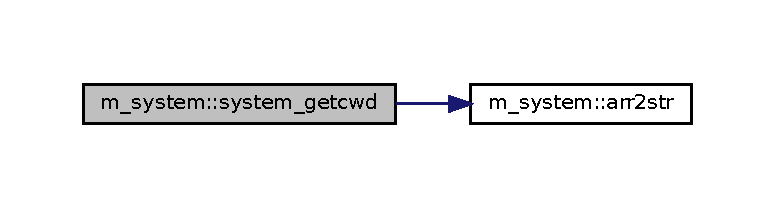
\includegraphics[width=350pt]{namespacem__system_a5a32db818a9ffb0a4ea724e95356c560_cgraph}
\end{center}
\end{figure}
\mbox{\Hypertarget{namespacem__system_a15f307db605f8b332d4213814c0fb1a9}\label{namespacem__system_a15f307db605f8b332d4213814c0fb1a9}} 
\index{m\+\_\+system@{m\+\_\+system}!system\+\_\+getenv@{system\+\_\+getenv}}
\index{system\+\_\+getenv@{system\+\_\+getenv}!m\+\_\+system@{m\+\_\+system}}
\subsubsection{\texorpdfstring{system\+\_\+getenv()}{system\_getenv()}}
{\footnotesize\ttfamily character(len=\+:) function, allocatable, public m\+\_\+system\+::system\+\_\+getenv (\begin{DoxyParamCaption}\item[{character(len=$\ast$), intent(in)}]{name }\end{DoxyParamCaption})}



\subsubsection*{N\+A\+ME}

system\+\_\+getenv(3f) -\/ \mbox{[}M\+\_\+system\+:E\+N\+V\+I\+R\+O\+N\+M\+E\+NT\mbox{]} get environment variable from Fortran by calling get\+\_\+environment\+\_\+variable(3f) (L\+I\+C\+E\+N\+SE\+:PD) 

\subsubsection*{S\+Y\+N\+O\+P\+S\+IS}

\begin{DoxyVerb}function system_getenv(name)

 character(len=:),allocatable   :: system_getenv
 character(len=*),intent(in)    :: name
\end{DoxyVerb}


\subsubsection*{D\+E\+S\+C\+R\+I\+P\+T\+I\+ON}

The \mbox{\hyperlink{namespacem__system_a15f307db605f8b332d4213814c0fb1a9}{system\+\_\+getenv()}} function gets the value of an environment variable.

\subsubsection*{O\+P\+T\+I\+O\+NS}

name Return the value of the specified environment variable or blank if the variable is not defined.

\subsubsection*{E\+X\+A\+M\+P\+LE}

Sample setting an environment variable from Fortran\+:

program demo\+\_\+system\+\_\+getenv use M\+\_\+system, only \+: system\+\_\+getenv implicit none integer \+:\+: ierr

write($\ast$,\textquotesingle{}(\char`\"{}\+U\+S\+E\+R     \+: \char`\"{},a)\textquotesingle{})system\+\_\+getenv(\textquotesingle{}U\+S\+ER\textquotesingle{}) write($\ast$,\textquotesingle{}(\char`\"{}\+L\+O\+G\+N\+A\+M\+E  \+: \char`\"{},a)\textquotesingle{})system\+\_\+getenv(\textquotesingle{}L\+O\+G\+N\+A\+ME\textquotesingle{}) write($\ast$,\textquotesingle{}(\char`\"{}\+U\+S\+E\+R\+N\+A\+M\+E \+: \char`\"{},a)\textquotesingle{})system\+\_\+getenv(\textquotesingle{}U\+S\+E\+R\+N\+A\+ME\textquotesingle{})

end program demo\+\_\+system\+\_\+getenv

\subsubsection*{A\+U\+T\+H\+OR}

John S. Urban \subsubsection*{L\+I\+C\+E\+N\+SE}

Public Domain \mbox{\Hypertarget{namespacem__system_aec137429fbb8c848db4ecd914466d7e8}\label{namespacem__system_aec137429fbb8c848db4ecd914466d7e8}} 
\index{m\+\_\+system@{m\+\_\+system}!system\+\_\+getgrgid@{system\+\_\+getgrgid}}
\index{system\+\_\+getgrgid@{system\+\_\+getgrgid}!m\+\_\+system@{m\+\_\+system}}
\subsubsection{\texorpdfstring{system\+\_\+getgrgid()}{system\_getgrgid()}}
{\footnotesize\ttfamily character(len=\+:) function, allocatable, public m\+\_\+system\+::system\+\_\+getgrgid (\begin{DoxyParamCaption}\item[{class($\ast$), intent(in)}]{gid }\end{DoxyParamCaption})}



\subsubsection*{N\+A\+ME}

system\+\_\+getgrgid(3f) -\/ \mbox{[}M\+\_\+system\+:Q\+U\+E\+RY\mbox{]} get groupd name associated with a G\+ID (L\+I\+C\+E\+N\+SE\+:PD) \subsubsection*{S\+Y\+N\+O\+P\+S\+IS}

function system\+\_\+getgrgid(gid) result (gname)

class($\ast$),intent(in) \+:\+: gid ! any I\+N\+T\+E\+G\+ER type character(len=\+:),allocatable \+:\+: gname

\subsubsection*{D\+E\+S\+C\+R\+I\+P\+T\+I\+ON}

\begin{DoxyVerb}The system_getlogin() function returns a string containing the group
name associated with the given GID. If no match is found
it returns a null string and sets errno to indicate the error.
\end{DoxyVerb}


\subsubsection*{O\+P\+T\+I\+ON}

gid G\+ID to try to look up associated group for. Can be of any I\+N\+T\+E\+G\+ER type.

\subsubsection*{R\+E\+T\+U\+RN V\+A\+L\+UE}

gname returns the group name. Blank if an error occurs

\subsubsection*{E\+X\+A\+M\+P\+LE}

Sample program\+:

program demo\+\_\+system\+\_\+getgrgid use M\+\_\+system, only \+: system\+\_\+getgrgid use M\+\_\+system, only \+: \mbox{\hyperlink{interfacem__system_1_1system__getgid}{system\+\_\+getgid}} implicit none character(len=\+:),allocatable \+:\+: name name=system\+\_\+getgrgid( system\+\_\+getgid() ) write($\ast$,\textquotesingle{}(\char`\"{}group\mbox{[}\char`\"{},a,\char`\"{}\mbox{]} for \char`\"{},i0)\textquotesingle{})name,system\+\_\+getgid() end program demo\+\_\+system\+\_\+getgrgid

Results\+:

group\mbox{[}default\mbox{]} for 197121

\subsubsection*{A\+U\+T\+H\+OR}

John S. Urban \subsubsection*{L\+I\+C\+E\+N\+SE}

Public Domain 

References anyinteger\+\_\+to\+\_\+64bit(), and arr2str().

Here is the call graph for this function\+:
\nopagebreak
\begin{figure}[H]
\begin{center}
\leavevmode
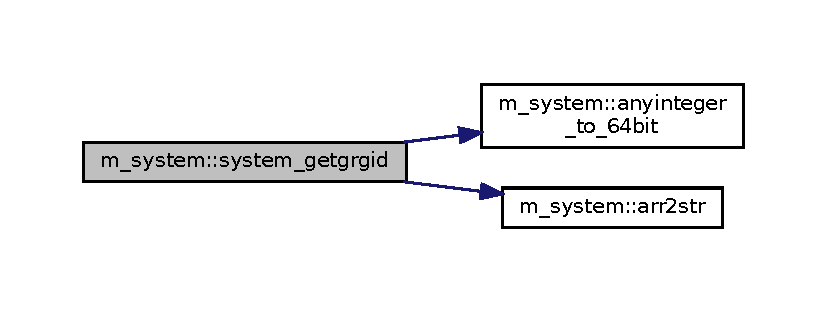
\includegraphics[width=350pt]{namespacem__system_aec137429fbb8c848db4ecd914466d7e8_cgraph}
\end{center}
\end{figure}
\mbox{\Hypertarget{namespacem__system_a96fab225737afb77ff1cbba9866f0d05}\label{namespacem__system_a96fab225737afb77ff1cbba9866f0d05}} 
\index{m\+\_\+system@{m\+\_\+system}!system\+\_\+gethostname@{system\+\_\+gethostname}}
\index{system\+\_\+gethostname@{system\+\_\+gethostname}!m\+\_\+system@{m\+\_\+system}}
\subsubsection{\texorpdfstring{system\+\_\+gethostname()}{system\_gethostname()}}
{\footnotesize\ttfamily subroutine, public m\+\_\+system\+::system\+\_\+gethostname (\begin{DoxyParamCaption}\item[{character(len=\+:), intent(out), allocatable}]{N\+A\+ME,  }\item[{integer, intent(out)}]{I\+E\+RR }\end{DoxyParamCaption})}



\subsubsection*{N\+A\+ME}

system\+\_\+gethostname(3f) -\/ \mbox{[}M\+\_\+system\+:Q\+U\+E\+RY\mbox{]} get name of current host (L\+I\+C\+E\+N\+SE\+:PD) \subsubsection*{S\+Y\+N\+O\+P\+S\+IS}

subroutine system\+\_\+gethostname(string,ierr)

character(len=\+:),allocatable,intent(out) \+:\+: N\+A\+ME integer,intent(out) \+:\+: I\+E\+RR \subsubsection*{D\+E\+S\+C\+R\+I\+P\+T\+I\+ON}

The system\+\_\+gethostname(3f) procedure returns the standard host name for the current machine.

\subsubsection*{O\+P\+T\+I\+O\+NS}

string returns the hostname. Must be an allocatable C\+H\+A\+R\+A\+C\+T\+ER variable. ierr Upon successful completion, 0 shall be returned; otherwise, -\/1 shall be returned. \subsubsection*{E\+X\+A\+M\+P\+LE}

Sample program\+:

program demo\+\_\+system\+\_\+gethostname

use M\+\_\+system, only \+: system\+\_\+gethostname implicit none character(len=\+:),allocatable \+:\+: name integer \+:\+: ierr

call system\+\_\+gethostname(name,ierr) if(ierr.\+eq.\+0)then write($\ast$,\textquotesingle{}(\char`\"{}hostname\mbox{[}\char`\"{},a,\char`\"{}\mbox{]}\char`\"{})\textquotesingle{})name else write($\ast$,\textquotesingle{}(a)\textquotesingle{})\textquotesingle{}E\+R\+R\+OR\+: could not get hostname\textquotesingle{} endif

end program demo\+\_\+system\+\_\+gethostname

\subsubsection*{A\+U\+T\+H\+OR}

John S. Urban \subsubsection*{L\+I\+C\+E\+N\+SE}

Public Domain 

References arr2str(), and host\+\_\+name\+\_\+max.

Here is the call graph for this function\+:
\nopagebreak
\begin{figure}[H]
\begin{center}
\leavevmode
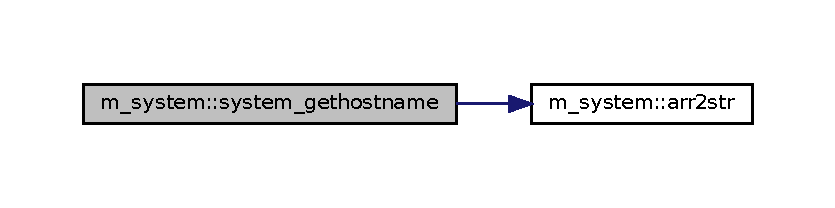
\includegraphics[width=350pt]{namespacem__system_a96fab225737afb77ff1cbba9866f0d05_cgraph}
\end{center}
\end{figure}
\mbox{\Hypertarget{namespacem__system_a70f78645a1f130734005e190d469529d}\label{namespacem__system_a70f78645a1f130734005e190d469529d}} 
\index{m\+\_\+system@{m\+\_\+system}!system\+\_\+getlogin@{system\+\_\+getlogin}}
\index{system\+\_\+getlogin@{system\+\_\+getlogin}!m\+\_\+system@{m\+\_\+system}}
\subsubsection{\texorpdfstring{system\+\_\+getlogin()}{system\_getlogin()}}
{\footnotesize\ttfamily character(len=\+:) function, allocatable, public m\+\_\+system\+::system\+\_\+getlogin (\begin{DoxyParamCaption}{ }\end{DoxyParamCaption})}



\subsubsection*{N\+A\+ME}

system\+\_\+getlogin(3f) -\/ \mbox{[}M\+\_\+system\+:Q\+U\+E\+RY\mbox{]} get login name (L\+I\+C\+E\+N\+SE\+:PD) 

\subsubsection*{S\+Y\+N\+O\+P\+S\+IS}

function \mbox{\hyperlink{namespacem__system_a70f78645a1f130734005e190d469529d}{system\+\_\+getlogin()}} result (fname)

character(len=\+:),allocatable \+:\+: F\+N\+A\+ME

\subsubsection*{D\+E\+S\+C\+R\+I\+P\+T\+I\+ON}

\begin{DoxyVerb}The system_getlogin() function returns a string containing the user
name associated by the login activity with the controlling terminal
of the current process. Otherwise, it returns a null string and sets
errno to indicate the error.

Three names associated with the current process can be determined:
   o system_getpwuid(system_getuid()) returns the name associated with the real user ID of the process.
   o system_getpwuid(system_geteuid()) returns the name associated with the effective user ID of the process
   o system_getlogin() returns the name associated with the current login activity
\end{DoxyVerb}


\subsubsection*{R\+E\+T\+U\+RN V\+A\+L\+UE}

fname returns the login name.

\subsubsection*{E\+X\+A\+M\+P\+LE}

Sample program\+:

program demo\+\_\+system\+\_\+getlogin use M\+\_\+system, only \+: system\+\_\+getlogin implicit none character(len=\+:),allocatable \+:\+: name name=\mbox{\hyperlink{namespacem__system_a70f78645a1f130734005e190d469529d}{system\+\_\+getlogin()}} write($\ast$,\textquotesingle{}(\char`\"{}login\mbox{[}\char`\"{},a,\char`\"{}\mbox{]}\char`\"{})\textquotesingle{})name end program demo\+\_\+system\+\_\+getlogin

Results\+:

login\mbox{[}J\+SU\mbox{]}

\subsubsection*{A\+U\+T\+H\+OR}

John S. Urban \subsubsection*{L\+I\+C\+E\+N\+SE}

Public Domain 

References c2f\+\_\+string(), and system\+\_\+getpwuid().

Here is the call graph for this function\+:
\nopagebreak
\begin{figure}[H]
\begin{center}
\leavevmode
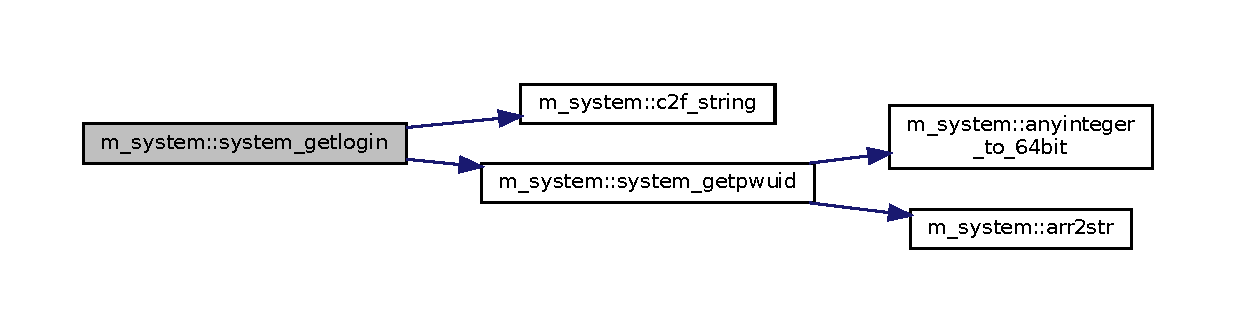
\includegraphics[width=350pt]{namespacem__system_a70f78645a1f130734005e190d469529d_cgraph}
\end{center}
\end{figure}
\mbox{\Hypertarget{namespacem__system_a59cd13de95dc9a65b444f02614ea39ce}\label{namespacem__system_a59cd13de95dc9a65b444f02614ea39ce}} 
\index{m\+\_\+system@{m\+\_\+system}!system\+\_\+getpwuid@{system\+\_\+getpwuid}}
\index{system\+\_\+getpwuid@{system\+\_\+getpwuid}!m\+\_\+system@{m\+\_\+system}}
\subsubsection{\texorpdfstring{system\+\_\+getpwuid()}{system\_getpwuid()}}
{\footnotesize\ttfamily character(len=\+:) function, allocatable, public m\+\_\+system\+::system\+\_\+getpwuid (\begin{DoxyParamCaption}\item[{class($\ast$), intent(in)}]{uid }\end{DoxyParamCaption})}



\subsubsection*{N\+A\+ME}

system\+\_\+getpwuid(3f) -\/ \mbox{[}M\+\_\+system\+:Q\+U\+E\+RY\mbox{]} get login name associated with a U\+ID (L\+I\+C\+E\+N\+SE\+:PD) \subsubsection*{S\+Y\+N\+O\+P\+S\+IS}

function system\+\_\+getpwuid(uid) result (uname)

class($\ast$),intent(in) \+:\+: uid ! any I\+N\+T\+E\+G\+ER type character(len=\+:),allocatable \+:\+: uname

\subsubsection*{D\+E\+S\+C\+R\+I\+P\+T\+I\+ON}

\begin{DoxyVerb}The system_getpwuid() function returns a string containing the user
name associated with the given UID. If no match is found it returns
a null string and sets errno to indicate the error.
\end{DoxyVerb}


\subsubsection*{O\+P\+T\+I\+ON}

uid U\+ID to try to look up associated username for. Can be of any I\+N\+T\+E\+G\+ER type.

\subsubsection*{R\+E\+T\+U\+RN V\+A\+L\+UE}

uname returns the login name.

\subsubsection*{E\+X\+A\+M\+P\+LE}

Sample program\+:

program demo\+\_\+system\+\_\+getpwuid use M\+\_\+system, only \+: system\+\_\+getpwuid use M\+\_\+system, only \+: \mbox{\hyperlink{interfacem__system_1_1system__getuid}{system\+\_\+getuid}} use,intrinsic \+:\+: iso\+\_\+fortran\+\_\+env, only \+: int64 implicit none character(len=\+:),allocatable \+:\+: name integer(kind=int64) \+:\+: uid uid=system\+\_\+getuid() name=system\+\_\+getpwuid(uid) write($\ast$,\textquotesingle{}(\char`\"{}login\mbox{[}\char`\"{},a,\char`\"{}\mbox{]} has U\+I\+D \char`\"{},i0)\textquotesingle{})name,uid end program demo\+\_\+system\+\_\+getpwuid

\subsubsection*{A\+U\+T\+H\+OR}

John S. Urban \subsubsection*{L\+I\+C\+E\+N\+SE}

Public Domain 

References anyinteger\+\_\+to\+\_\+64bit(), and arr2str().

Here is the call graph for this function\+:
\nopagebreak
\begin{figure}[H]
\begin{center}
\leavevmode
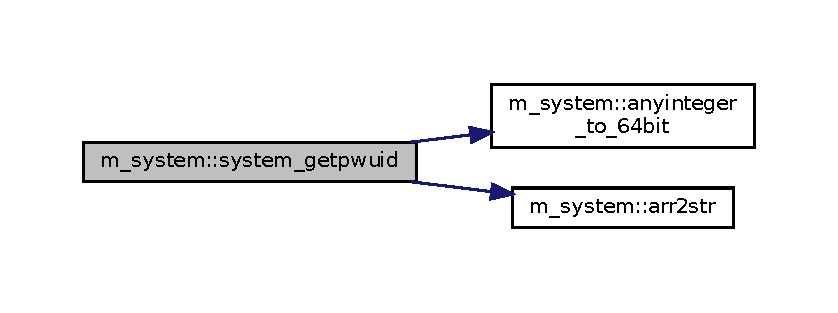
\includegraphics[width=350pt]{namespacem__system_a59cd13de95dc9a65b444f02614ea39ce_cgraph}
\end{center}
\end{figure}
Here is the caller graph for this function\+:
\nopagebreak
\begin{figure}[H]
\begin{center}
\leavevmode
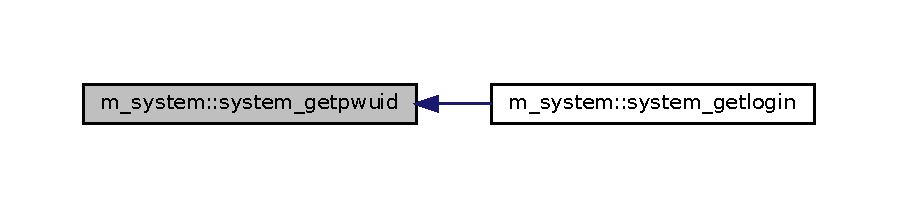
\includegraphics[width=350pt]{namespacem__system_a59cd13de95dc9a65b444f02614ea39ce_icgraph}
\end{center}
\end{figure}
\mbox{\Hypertarget{namespacem__system_aa9ca951be39d2ea738d627cf42c00ddd}\label{namespacem__system_aa9ca951be39d2ea738d627cf42c00ddd}} 
\index{m\+\_\+system@{m\+\_\+system}!system\+\_\+getumask@{system\+\_\+getumask}}
\index{system\+\_\+getumask@{system\+\_\+getumask}!m\+\_\+system@{m\+\_\+system}}
\subsubsection{\texorpdfstring{system\+\_\+getumask()}{system\_getumask()}}
{\footnotesize\ttfamily integer function, public m\+\_\+system\+::system\+\_\+getumask (\begin{DoxyParamCaption}{ }\end{DoxyParamCaption})}



\subsubsection*{N\+A\+ME}

system\+\_\+getumask(3f) -\/ \mbox{[}M\+\_\+system\mbox{]} get current umask (L\+I\+C\+E\+N\+SE\+:PD) \subsubsection*{S\+Y\+N\+O\+P\+S\+IS}

integer function \mbox{\hyperlink{namespacem__system_aa9ca951be39d2ea738d627cf42c00ddd}{system\+\_\+getumask()}} result (umask\+\_\+value) \subsubsection*{D\+E\+S\+C\+R\+I\+P\+T\+I\+ON}

The return value from getumask(3f) is the value of the file creation mask, obtained by using umask(3c). \subsubsection*{E\+X\+A\+M\+P\+LE}

Sample program

program demo\+\_\+getumask use M\+\_\+system, only \+: system\+\_\+getumask, system\+\_\+setumask integer \+:\+: i write($\ast$,101)(\mbox{\hyperlink{namespacem__system_aa9ca951be39d2ea738d627cf42c00ddd}{system\+\_\+getumask()}},i=1,4) 101 format(1x,i0,1x,\char`\"{}\+O\textquotesingle{}\char`\"{},o4.\+4,\char`\"{}\textquotesingle{}\char`\"{},1x,\textquotesingle{}Z\char`\"{}\textquotesingle{},z0,\char`\"{}\textquotesingle{}\char`\"{},1x,\char`\"{}B\textquotesingle{}\char`\"{},b12.\+12,\char`\"{}\textquotesingle{}") end program demo\+\_\+getumask

Expected output

18 O\textquotesingle{}022\textquotesingle{} Z\char`\"{}12\textquotesingle{} B\textquotesingle{}000010010\char`\"{} \mbox{\Hypertarget{namespacem__system_a791fa587005ec07cbcd7b0045ee6f43f}\label{namespacem__system_a791fa587005ec07cbcd7b0045ee6f43f}} 
\index{m\+\_\+system@{m\+\_\+system}!system\+\_\+isblk@{system\+\_\+isblk}}
\index{system\+\_\+isblk@{system\+\_\+isblk}!m\+\_\+system@{m\+\_\+system}}
\subsubsection{\texorpdfstring{system\+\_\+isblk()}{system\_isblk()}}
{\footnotesize\ttfamily logical function, public m\+\_\+system\+::system\+\_\+isblk (\begin{DoxyParamCaption}\item[{character(len=$\ast$), intent(in)}]{pathname }\end{DoxyParamCaption})}



\subsubsection*{N\+A\+ME}

system\+\_\+isblk(3f) -\/ \mbox{[}M\+\_\+system\mbox{]} checks if argument is a block device (L\+I\+C\+E\+N\+SE\+:PD) 

\subsubsection*{S\+Y\+N\+O\+P\+S\+IS}

logical function system\+\_\+isblk(pathname)

character(len=$\ast$),intent(in) \+:\+: pathname logical \+:\+: system\+\_\+isblk

\subsubsection*{D\+E\+S\+C\+R\+I\+P\+T\+I\+ON}

The isblk(3f) function checks if path is a path to a block device.

\subsubsection*{O\+P\+T\+I\+O\+NS}

path a character string representing a block device pathname. Trailing spaces are ignored.

\subsubsection*{R\+E\+T\+U\+RN V\+A\+L\+UE}

The \mbox{\hyperlink{namespacem__system_a791fa587005ec07cbcd7b0045ee6f43f}{system\+\_\+isblk()}} function should always be successful and no return value is reserved to indicate an error.

\subsubsection*{E\+R\+R\+O\+RS}

No errors are defined.

\subsubsection*{S\+EE A\+L\+SO}

system\+\_\+isreg(3f), system\+\_\+stat(3f), system\+\_\+isdir(3f), system\+\_\+perm(3f)

\subsubsection*{E\+X\+A\+M\+P\+LE}

check if filename is a block device

program demo\+\_\+system\+\_\+isblk Use M\+\_\+system, only \+: system\+\_\+isblk implicit none integer \+:\+: i character(len=80),parameter \+:\+: names($\ast$)=\mbox{[} \& \textquotesingle{}/tmp \textquotesingle{}, \& \textquotesingle{}/tmp/\+N\+O\+T\+T\+H\+E\+RE \textquotesingle{}, \& \textquotesingle{}/usr/local \textquotesingle{}, \& \textquotesingle{}. \textquotesingle{}, \& \textquotesingle{}block\+\_\+device.\+tst\textquotesingle{}, \& \textquotesingle{}P\+R\+O\+B\+A\+B\+L\+Y\+\_\+\+N\+OT \textquotesingle{}\mbox{]} do i=1,size(names) write($\ast$,$\ast$)\textquotesingle{} is \textquotesingle{},trim(names(i)),\textquotesingle{} a block device? \textquotesingle{}, system\+\_\+isblk(names(i)) enddo end program demo\+\_\+system\+\_\+isblk

Results\+: 

References str2arr().

Here is the call graph for this function\+:
\nopagebreak
\begin{figure}[H]
\begin{center}
\leavevmode
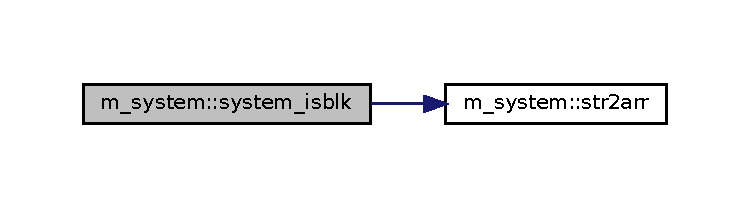
\includegraphics[width=350pt]{namespacem__system_a791fa587005ec07cbcd7b0045ee6f43f_cgraph}
\end{center}
\end{figure}
\mbox{\Hypertarget{namespacem__system_a12a948fa4aacda084a538ae3a5ae3cc6}\label{namespacem__system_a12a948fa4aacda084a538ae3a5ae3cc6}} 
\index{m\+\_\+system@{m\+\_\+system}!system\+\_\+ischr@{system\+\_\+ischr}}
\index{system\+\_\+ischr@{system\+\_\+ischr}!m\+\_\+system@{m\+\_\+system}}
\subsubsection{\texorpdfstring{system\+\_\+ischr()}{system\_ischr()}}
{\footnotesize\ttfamily logical function, public m\+\_\+system\+::system\+\_\+ischr (\begin{DoxyParamCaption}\item[{character(len=$\ast$), intent(in)}]{pathname }\end{DoxyParamCaption})}



\subsubsection*{N\+A\+ME}

system\+\_\+ischr(3f) -\/ \mbox{[}M\+\_\+system\mbox{]} checks if argument is a character device (L\+I\+C\+E\+N\+SE\+:PD) 

\subsubsection*{S\+Y\+N\+O\+P\+S\+IS}

logical function system\+\_\+ischr(pathname)

character(len=$\ast$),intent(in) \+:\+: pathname logical \+:\+: system\+\_\+ischr

\subsubsection*{D\+E\+S\+C\+R\+I\+P\+T\+I\+ON}

The ischr(3f) function checks if path is a path to a character device.

\subsubsection*{O\+P\+T\+I\+O\+NS}

path a character string representing a character device pathname. Trailing spaces are ignored.

\subsubsection*{R\+E\+T\+U\+RN V\+A\+L\+UE}

The \mbox{\hyperlink{namespacem__system_a12a948fa4aacda084a538ae3a5ae3cc6}{system\+\_\+ischr()}} function should always be successful and no return value is reserved to indicate an error.

\subsubsection*{E\+R\+R\+O\+RS}

No errors are defined.

\subsubsection*{S\+EE A\+L\+SO}

system\+\_\+isreg(3f), system\+\_\+stat(3f), system\+\_\+isdir(3f), system\+\_\+perm(3f)

\subsubsection*{E\+X\+A\+M\+P\+LE}

check if filename is a character file

program demo\+\_\+system\+\_\+ischr Use M\+\_\+system, only \+: system\+\_\+ischr implicit none integer \+:\+: i character(len=80),parameter \+:\+: names($\ast$)=\mbox{[} \& \textquotesingle{}/tmp \textquotesingle{}, \& \textquotesingle{}/tmp/\+N\+O\+T\+T\+H\+E\+RE \textquotesingle{}, \& \textquotesingle{}/usr/local \textquotesingle{}, \& \textquotesingle{}. \textquotesingle{}, \& \textquotesingle{}char\+\_\+dev.\+test \textquotesingle{}, \& \textquotesingle{}P\+R\+O\+B\+A\+B\+L\+Y\+\_\+\+N\+OT \textquotesingle{}\mbox{]} do i=1,size(names) write($\ast$,$\ast$)\textquotesingle{} is \textquotesingle{},trim(names(i)),\textquotesingle{} a character device? \textquotesingle{}, system\+\_\+ischr(names(i)) enddo end program demo\+\_\+system\+\_\+ischr

Results\+: 

References str2arr().

Here is the call graph for this function\+:
\nopagebreak
\begin{figure}[H]
\begin{center}
\leavevmode
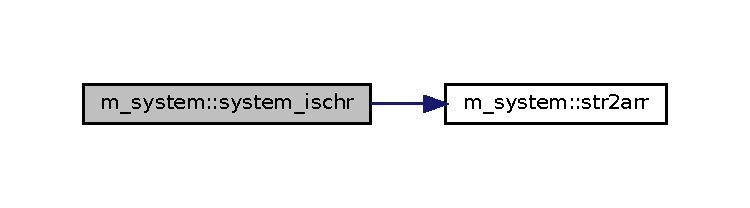
\includegraphics[width=350pt]{namespacem__system_a12a948fa4aacda084a538ae3a5ae3cc6_cgraph}
\end{center}
\end{figure}
\mbox{\Hypertarget{namespacem__system_ad097988a031e64b4f21f856cf45c9c73}\label{namespacem__system_ad097988a031e64b4f21f856cf45c9c73}} 
\index{m\+\_\+system@{m\+\_\+system}!system\+\_\+isdir@{system\+\_\+isdir}}
\index{system\+\_\+isdir@{system\+\_\+isdir}!m\+\_\+system@{m\+\_\+system}}
\subsubsection{\texorpdfstring{system\+\_\+isdir()}{system\_isdir()}}
{\footnotesize\ttfamily logical function, public m\+\_\+system\+::system\+\_\+isdir (\begin{DoxyParamCaption}\item[{character(len=$\ast$), intent(in)}]{dirname }\end{DoxyParamCaption})}



\subsubsection*{N\+A\+ME}

system\+\_\+isdir(3f) -\/ \mbox{[}M\+\_\+system\mbox{]} checks if argument is a directory path (L\+I\+C\+E\+N\+SE\+:PD) 

\subsubsection*{S\+Y\+N\+O\+P\+S\+IS}

logical function system\+\_\+isdir(pathname)

character(len=$\ast$),intent(in) \+:\+: pathname logical \+:\+: system\+\_\+isdir

\subsubsection*{D\+E\+S\+C\+R\+I\+P\+T\+I\+ON}

The system\+\_\+isdir(3f) function checks if path is a directory.

\subsubsection*{O\+P\+T\+I\+O\+NS}

path a character string representing a directory pathname. Trailing spaces are ignored.

\subsubsection*{R\+E\+T\+U\+RN V\+A\+L\+UE}

The \mbox{\hyperlink{namespacem__system_ad097988a031e64b4f21f856cf45c9c73}{system\+\_\+isdir()}} function should always be successful and no return value is reserved to indicate an error.

\subsubsection*{E\+R\+R\+O\+RS}

No errors are defined.

\subsubsection*{S\+EE A\+L\+SO}

system\+\_\+islnk(3f), system\+\_\+stat(3f), isreg(3f), system\+\_\+perm(3f)

\subsubsection*{E\+X\+A\+M\+P\+LE}

check if filename is a directory

program demo\+\_\+system\+\_\+isdir Use M\+\_\+system, only \+: system\+\_\+isdir implicit none integer \+:\+: i character(len=80),parameter \+:\+: names($\ast$)=\mbox{[} \& \textquotesingle{}/tmp \textquotesingle{}, \& \textquotesingle{}/tmp/\+N\+O\+T\+T\+H\+E\+RE \textquotesingle{}, \& \textquotesingle{}/usr/local \textquotesingle{}, \& \textquotesingle{}. \textquotesingle{}, \& \textquotesingle{}P\+R\+O\+B\+A\+B\+L\+Y\+\_\+\+N\+OT \textquotesingle{}\mbox{]} do i=1,size(names) write($\ast$,$\ast$)\textquotesingle{} is \textquotesingle{},trim(names(i)),\textquotesingle{} a directory? \textquotesingle{}, system\+\_\+isdir(names(i)) enddo end program demo\+\_\+system\+\_\+isdir

Results\+:

is /tmp a directory? T is /tmp/\+N\+O\+T\+T\+H\+E\+RE a directory? F is /usr/local a directory? T is . a directory? T is P\+R\+O\+B\+A\+B\+L\+Y\+\_\+\+N\+OT a directory? F 

References str2arr().

Here is the call graph for this function\+:
\nopagebreak
\begin{figure}[H]
\begin{center}
\leavevmode
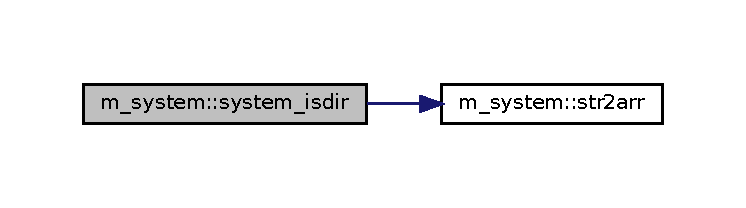
\includegraphics[width=350pt]{namespacem__system_ad097988a031e64b4f21f856cf45c9c73_cgraph}
\end{center}
\end{figure}
\mbox{\Hypertarget{namespacem__system_acbcaa0c5075ca103815f441ee410e1a3}\label{namespacem__system_acbcaa0c5075ca103815f441ee410e1a3}} 
\index{m\+\_\+system@{m\+\_\+system}!system\+\_\+isfifo@{system\+\_\+isfifo}}
\index{system\+\_\+isfifo@{system\+\_\+isfifo}!m\+\_\+system@{m\+\_\+system}}
\subsubsection{\texorpdfstring{system\+\_\+isfifo()}{system\_isfifo()}}
{\footnotesize\ttfamily logical function, public m\+\_\+system\+::system\+\_\+isfifo (\begin{DoxyParamCaption}\item[{character(len=$\ast$), intent(in)}]{pathname }\end{DoxyParamCaption})}



\subsubsection*{N\+A\+ME}

system\+\_\+isfifo(3f) -\/ \mbox{[}M\+\_\+system\mbox{]} checks if argument is a fifo -\/ named pipe (L\+I\+C\+E\+N\+SE\+:PD) 

\subsubsection*{S\+Y\+N\+O\+P\+S\+IS}

logical function system\+\_\+isfifo(pathname)

character(len=$\ast$),intent(in) \+:\+: pathname logical \+:\+: system\+\_\+isfifo

\subsubsection*{D\+E\+S\+C\+R\+I\+P\+T\+I\+ON}

The isfifo(3f) function checks if path is a path to a fifo -\/ named pipe.

\subsubsection*{O\+P\+T\+I\+O\+NS}

path a character string representing a fifo -\/ named pipe pathname. Trailing spaces are ignored.

\subsubsection*{R\+E\+T\+U\+RN V\+A\+L\+UE}

The \mbox{\hyperlink{namespacem__system_acbcaa0c5075ca103815f441ee410e1a3}{system\+\_\+isfifo()}} function should always be successful and no return value is reserved to indicate an error.

\subsubsection*{E\+R\+R\+O\+RS}

No errors are defined.

\subsubsection*{S\+EE A\+L\+SO}

system\+\_\+isreg(3f), system\+\_\+stat(3f), system\+\_\+isdir(3f), system\+\_\+perm(3f)

\subsubsection*{E\+X\+A\+M\+P\+LE}

check if filename is a F\+I\+FO file

program demo\+\_\+system\+\_\+isfifo Use M\+\_\+system, only \+: system\+\_\+isfifo implicit none integer \+:\+: i character(len=80),parameter \+:\+: names($\ast$)=\mbox{[} \& \textquotesingle{}/tmp \textquotesingle{}, \& \textquotesingle{}/tmp/\+N\+O\+T\+T\+H\+E\+RE \textquotesingle{}, \& \textquotesingle{}/usr/local \textquotesingle{}, \& \textquotesingle{}. \textquotesingle{}, \& \textquotesingle{}fifo.\+test \textquotesingle{}, \& \textquotesingle{}P\+R\+O\+B\+A\+B\+L\+Y\+\_\+\+N\+OT \textquotesingle{}\mbox{]} do i=1,size(names) write($\ast$,$\ast$)\textquotesingle{} is \textquotesingle{},trim(names(i)),\textquotesingle{} a fifo(named pipe)? \textquotesingle{}, system\+\_\+isfifo(names(i)) enddo end program demo\+\_\+system\+\_\+isfifo 

References str2arr().

Here is the call graph for this function\+:
\nopagebreak
\begin{figure}[H]
\begin{center}
\leavevmode
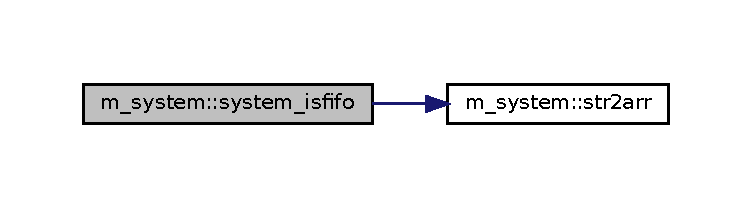
\includegraphics[width=350pt]{namespacem__system_acbcaa0c5075ca103815f441ee410e1a3_cgraph}
\end{center}
\end{figure}
\mbox{\Hypertarget{namespacem__system_ab05694cc3d76a3ecc87e4b4490c4c217}\label{namespacem__system_ab05694cc3d76a3ecc87e4b4490c4c217}} 
\index{m\+\_\+system@{m\+\_\+system}!system\+\_\+islnk@{system\+\_\+islnk}}
\index{system\+\_\+islnk@{system\+\_\+islnk}!m\+\_\+system@{m\+\_\+system}}
\subsubsection{\texorpdfstring{system\+\_\+islnk()}{system\_islnk()}}
{\footnotesize\ttfamily logical function, public m\+\_\+system\+::system\+\_\+islnk (\begin{DoxyParamCaption}\item[{character(len=$\ast$), intent(in)}]{pathname }\end{DoxyParamCaption})}



\subsubsection*{N\+A\+ME}

system\+\_\+islnk(3f) -\/ \mbox{[}M\+\_\+system\mbox{]} checks if argument is a link (L\+I\+C\+E\+N\+SE\+:PD) 

\subsubsection*{S\+Y\+N\+O\+P\+S\+IS}

\begin{DoxyVerb}logical function system_islnk(pathname)

character(len=*),intent(in) :: pathname
logical                     :: system_islnk
\end{DoxyVerb}


\subsubsection*{D\+E\+S\+C\+R\+I\+P\+T\+I\+ON}

The islnk(3f) function checks if path is a path to a link.

\subsubsection*{O\+P\+T\+I\+O\+NS}

path a character string representing a link pathname. Trailing spaces are ignored.

\subsubsection*{R\+E\+T\+U\+RN V\+A\+L\+UE}

The \mbox{\hyperlink{namespacem__system_ab05694cc3d76a3ecc87e4b4490c4c217}{system\+\_\+islnk()}} function should always be successful and no return value is reserved to indicate an error.

\subsubsection*{E\+R\+R\+O\+RS}

No errors are defined.

\subsubsection*{S\+EE A\+L\+SO}

system\+\_\+isreg(3f), system\+\_\+stat(3f), system\+\_\+isdir(3f), system\+\_\+perm(3f)

\subsubsection*{E\+X\+A\+M\+P\+LE}

Sample program\+:

program demo\+\_\+system\+\_\+islnk Use M\+\_\+system, only \+: system\+\_\+islnk implicit none integer \+:\+: i character(len=80),parameter \+:\+: names($\ast$)=\mbox{[} \& \textquotesingle{}/tmp \textquotesingle{}, \& \textquotesingle{}/tmp/\+N\+O\+T\+T\+H\+E\+RE \textquotesingle{}, \& \textquotesingle{}/usr/local \textquotesingle{}, \& \textquotesingle{}. \textquotesingle{}, \& \textquotesingle{}link.\+test \textquotesingle{}, \& \textquotesingle{}P\+R\+O\+B\+A\+B\+L\+Y\+\_\+\+N\+OT \textquotesingle{}\mbox{]} do i=1,size(names) write($\ast$,$\ast$)\textquotesingle{} is \textquotesingle{},trim(names(i)),\textquotesingle{} a link? \textquotesingle{}, system\+\_\+islnk(names(i)) enddo end program demo\+\_\+system\+\_\+islnk

Results\+: 

References str2arr().

Here is the call graph for this function\+:
\nopagebreak
\begin{figure}[H]
\begin{center}
\leavevmode
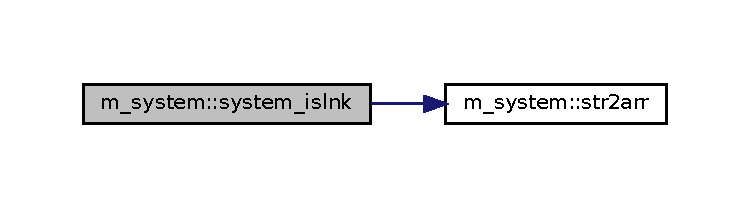
\includegraphics[width=350pt]{namespacem__system_ab05694cc3d76a3ecc87e4b4490c4c217_cgraph}
\end{center}
\end{figure}
\mbox{\Hypertarget{namespacem__system_a127bdd84ccd4b52f3f29abbc56af029b}\label{namespacem__system_a127bdd84ccd4b52f3f29abbc56af029b}} 
\index{m\+\_\+system@{m\+\_\+system}!system\+\_\+isreg@{system\+\_\+isreg}}
\index{system\+\_\+isreg@{system\+\_\+isreg}!m\+\_\+system@{m\+\_\+system}}
\subsubsection{\texorpdfstring{system\+\_\+isreg()}{system\_isreg()}}
{\footnotesize\ttfamily logical function, public m\+\_\+system\+::system\+\_\+isreg (\begin{DoxyParamCaption}\item[{character(len=$\ast$), intent(in)}]{pathname }\end{DoxyParamCaption})}



\subsubsection*{N\+A\+ME}

system\+\_\+isreg(3f) -\/ \mbox{[}M\+\_\+system\mbox{]} checks if argument is a regular file (L\+I\+C\+E\+N\+SE\+:PD) 

\subsubsection*{S\+Y\+N\+O\+P\+S\+IS}

logical function system\+\_\+isreg(pathname)

character(len=$\ast$),intent(in) \+:\+: pathname logical \+:\+: system\+\_\+isreg

\subsubsection*{D\+E\+S\+C\+R\+I\+P\+T\+I\+ON}

The isreg(3f) function checks if path is a regular file

\subsubsection*{O\+P\+T\+I\+O\+NS}

path a character string representing a pathname. Trailing spaces are ignored.

\subsubsection*{R\+E\+T\+U\+RN V\+A\+L\+UE}

The \mbox{\hyperlink{namespacem__system_a127bdd84ccd4b52f3f29abbc56af029b}{system\+\_\+isreg()}} function should always be successful and no return value is reserved to indicate an error.

\subsubsection*{E\+R\+R\+O\+RS}

No errors are defined.

\subsubsection*{S\+EE A\+L\+SO}

system\+\_\+islnk(3f), system\+\_\+stat(3f), system\+\_\+isdir(3f), system\+\_\+perm(3f)

\subsubsection*{E\+X\+A\+M\+P\+LE}

check if filename is a regular file

program demo\+\_\+system\+\_\+isreg Use M\+\_\+system, only \+: system\+\_\+isreg implicit none integer \+:\+: i character(len=80),parameter \+:\+: names($\ast$)=\mbox{[} \& \textquotesingle{}/tmp \textquotesingle{}, \& \textquotesingle{}test.\+txt \textquotesingle{}, \& \textquotesingle{}. \textquotesingle{}\mbox{]} do i=1,size(names) write($\ast$,$\ast$)\textquotesingle{} is \textquotesingle{},trim(names(i)),\textquotesingle{} a regular file? \textquotesingle{}, system\+\_\+isreg(names(i)) enddo end program demo\+\_\+system\+\_\+isreg 

References str2arr().

Here is the call graph for this function\+:
\nopagebreak
\begin{figure}[H]
\begin{center}
\leavevmode
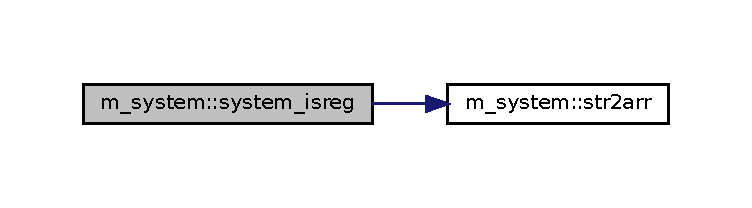
\includegraphics[width=350pt]{namespacem__system_a127bdd84ccd4b52f3f29abbc56af029b_cgraph}
\end{center}
\end{figure}
\mbox{\Hypertarget{namespacem__system_af6eb5074fe74552bc7a5e7d00f459087}\label{namespacem__system_af6eb5074fe74552bc7a5e7d00f459087}} 
\index{m\+\_\+system@{m\+\_\+system}!system\+\_\+issock@{system\+\_\+issock}}
\index{system\+\_\+issock@{system\+\_\+issock}!m\+\_\+system@{m\+\_\+system}}
\subsubsection{\texorpdfstring{system\+\_\+issock()}{system\_issock()}}
{\footnotesize\ttfamily logical function, public m\+\_\+system\+::system\+\_\+issock (\begin{DoxyParamCaption}\item[{character(len=$\ast$), intent(in)}]{pathname }\end{DoxyParamCaption})}



\subsubsection*{N\+A\+ME}

system\+\_\+issock(3f) -\/ \mbox{[}M\+\_\+system\mbox{]} checks if argument is a socket (L\+I\+C\+E\+N\+SE\+:PD) 

\subsubsection*{S\+Y\+N\+O\+P\+S\+IS}

logical function system\+\_\+issock(pathname)

character(len=$\ast$),intent(in) \+:\+: pathname logical \+:\+: system\+\_\+issock

\subsubsection*{D\+E\+S\+C\+R\+I\+P\+T\+I\+ON}

The issock(3f) function checks if path is a path to a socket

\subsubsection*{O\+P\+T\+I\+O\+NS}

path a character string representing a socket pathname. Trailing spaces are ignored.

\subsubsection*{R\+E\+T\+U\+RN V\+A\+L\+UE}

The \mbox{\hyperlink{namespacem__system_af6eb5074fe74552bc7a5e7d00f459087}{system\+\_\+issock()}} function should always be successful and no return value is reserved to indicate an error.

\subsubsection*{E\+R\+R\+O\+RS}

No errors are defined.

\subsubsection*{S\+EE A\+L\+SO}

system\+\_\+isreg(3f), system\+\_\+stat(3f), system\+\_\+isdir(3f), system\+\_\+perm(3f)

\subsubsection*{E\+X\+A\+M\+P\+LE}

check if filename is a socket

program demo\+\_\+system\+\_\+issock Use M\+\_\+system, only \+: system\+\_\+issock implicit none integer \+:\+: i character(len=80),parameter \+:\+: names($\ast$)=\mbox{[} \& \textquotesingle{}/tmp \textquotesingle{}, \& \textquotesingle{}/tmp/\+N\+O\+T\+T\+H\+E\+RE \textquotesingle{}, \& \textquotesingle{}/usr/local \textquotesingle{}, \& \textquotesingle{}. \textquotesingle{}, \& \textquotesingle{}sock.\+test \textquotesingle{}, \& \textquotesingle{}P\+R\+O\+B\+A\+B\+L\+Y\+\_\+\+N\+OT \textquotesingle{}\mbox{]} do i=1,size(names) write($\ast$,$\ast$)\textquotesingle{} is \textquotesingle{},trim(names(i)),\textquotesingle{} a socket? \textquotesingle{}, system\+\_\+issock(names(i)) enddo end program demo\+\_\+system\+\_\+issock 

References str2arr().

Here is the call graph for this function\+:
\nopagebreak
\begin{figure}[H]
\begin{center}
\leavevmode
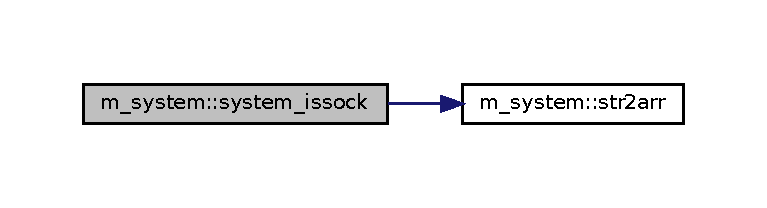
\includegraphics[width=350pt]{namespacem__system_af6eb5074fe74552bc7a5e7d00f459087_cgraph}
\end{center}
\end{figure}
\mbox{\Hypertarget{namespacem__system_aa77d9c9ae68750f515ba3d04d022c43c}\label{namespacem__system_aa77d9c9ae68750f515ba3d04d022c43c}} 
\index{m\+\_\+system@{m\+\_\+system}!system\+\_\+link@{system\+\_\+link}}
\index{system\+\_\+link@{system\+\_\+link}!m\+\_\+system@{m\+\_\+system}}
\subsubsection{\texorpdfstring{system\+\_\+link()}{system\_link()}}
{\footnotesize\ttfamily integer function, public m\+\_\+system\+::system\+\_\+link (\begin{DoxyParamCaption}\item[{character(len=$\ast$), intent(in)}]{oldname,  }\item[{character(len=$\ast$), intent(in)}]{newname }\end{DoxyParamCaption})}



\subsubsection*{N\+A\+ME}

system\+\_\+link(3f) -\/ \mbox{[}M\+\_\+system\mbox{]} link one file to another file relative to two directory file descriptors (L\+I\+C\+E\+N\+SE\+:PD) 

\subsubsection*{S\+Y\+N\+O\+P\+S\+IS}

\begin{DoxyVerb}integer function link(oldpath,newpath);

 character(len=*),intent(in) :: oldpath
 character(len=*),intent(in) :: newpath
\end{DoxyVerb}


\subsubsection*{D\+E\+S\+C\+R\+I\+P\+T\+I\+ON}

The link() function shall create a new link (directory entry) for the existing file, path1.

The path1 argument points to a pathname naming an existing file. The path2 argument points to a pathname naming the new directory entry to be created. The link() function shall atomically create a new link for the existing file and the link count of the file shall be incremented by one.

If path1 names a directory, link() shall fail unless the process has appropriate privileges and the implementation supports using link() on directories.

If path1 names a symbolic link, it is implementation-\/defined whether link() follows the symbolic link, or creates a new link to the symbolic link itself.

Upon successful completion, link() shall mark for update the last file status change timestamp of the file. Also, the last data modification and last file status change timestamps of the directory that contains the new entry shall be marked for update.

If link() fails, no link shall be created and the link count of the file shall remain unchanged.

The implementation may require that the calling process has permission to access the existing file.

The linkat() function shall be equivalent to the link() function except that symbolic links shall be handled as specified by the value of flag (see below) and except in the case where either path1 or path2 or both are relative paths. In this case a relative path path1 is interpreted relative to the directory associated with the file descriptor fd1 instead of the current working directory and similarly for path2 and the file descriptor fd2. If the file descriptor was opened without O\+\_\+\+S\+E\+A\+R\+CH, the function shall check whether directory searches are permitted using the current permissions of the directory underlying the file descriptor. If the file descriptor was opened with O\+\_\+\+S\+E\+A\+R\+CH, the function shall not perform the check.

Values for flag are constructed by a bitwise-\/inclusive OR of flags from the following list, defined in $<$fcntl.\+h$>$\+:

A\+T\+\_\+\+S\+Y\+M\+L\+I\+N\+K\+\_\+\+F\+O\+L\+L\+OW If path1 names a symbolic link, a new link for the target of the symbolic link is created.

If linkat() is passed the special value A\+T\+\_\+\+F\+D\+C\+WD in the fd1 or fd2 parameter, the current working directory shall be used for the respective path argument. If both fd1 and fd2 have value A\+T\+\_\+\+F\+D\+C\+WD, the behavior shall be identical to a call to link(), except that symbolic links shall be handled as specified by the value of flag.

Some implementations do allow links between file systems.

If path1 refers to a symbolic link, application developers should use linkat() with appropriate flags to select whether or not the symbolic link should be resolved.

If the A\+T\+\_\+\+S\+Y\+M\+L\+I\+N\+K\+\_\+\+F\+O\+L\+L\+OW flag is clear in the flag argument and the path1 argument names a symbolic link, a new link is created for the symbolic link path1 and not its target.

\subsubsection*{R\+E\+T\+U\+RN V\+A\+L\+UE}

Upon successful completion, these functions shall return 0. Otherwise, these functions shall return -\/1 and set errno to indicate the error.

\subsubsection*{E\+X\+A\+M\+P\+L\+ES}

Creating a Link to a File

program demo\+\_\+system\+\_\+link use M\+\_\+system, only \+: system\+\_\+link, system\+\_\+perror integer \+:\+: ierr ierr = system\+\_\+link(\textquotesingle{}myfile1\textquotesingle{},\textquotesingle{}myfile2\textquotesingle{}) if(ierr.\+ne.\+0)then call system\+\_\+perror(\textquotesingle{}{\itshape demo\+\_\+system\+\_\+link}\textquotesingle{}) endif end program demo\+\_\+system\+\_\+link 

References str2arr().

Here is the call graph for this function\+:
\nopagebreak
\begin{figure}[H]
\begin{center}
\leavevmode
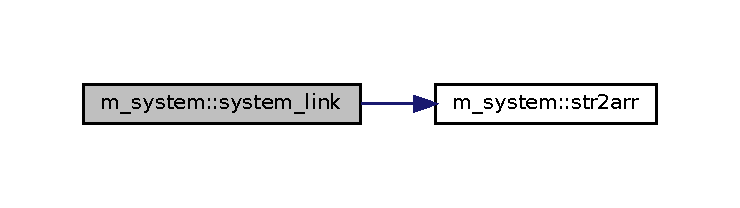
\includegraphics[width=350pt]{namespacem__system_aa77d9c9ae68750f515ba3d04d022c43c_cgraph}
\end{center}
\end{figure}
\mbox{\Hypertarget{namespacem__system_a084d644c236d22af2cc75c6e48fd6e96}\label{namespacem__system_a084d644c236d22af2cc75c6e48fd6e96}} 
\index{m\+\_\+system@{m\+\_\+system}!system\+\_\+mkdir@{system\+\_\+mkdir}}
\index{system\+\_\+mkdir@{system\+\_\+mkdir}!m\+\_\+system@{m\+\_\+system}}
\subsubsection{\texorpdfstring{system\+\_\+mkdir()}{system\_mkdir()}}
{\footnotesize\ttfamily integer function, public m\+\_\+system\+::system\+\_\+mkdir (\begin{DoxyParamCaption}\item[{character(len=$\ast$), intent(in)}]{dirname,  }\item[{integer, intent(in)}]{mode }\end{DoxyParamCaption})}



\subsubsection*{N\+A\+ME}

system\+\_\+mkdir(3f) -\/ \mbox{[}M\+\_\+system\mbox{]} call mkdir(3c) to create a new directory (L\+I\+C\+E\+N\+SE\+:PD) \subsubsection*{S\+Y\+N\+O\+P\+S\+IS}

\subsubsection*{D\+E\+S\+C\+R\+I\+P\+T\+I\+ON}

\begin{DoxyVerb}Predefined variables are typically used to set permission modes.
You can bytewise-OR together these variables to to create the most common
permissions mode:

 User:    R_USR  (read),  W_USR  (write),  X_USR(execute)
 Group:   R_GRP  (read),  W_GRP  (write),  X_GRP(execute)
 Others:  R_OTH  (read),  W_OTH  (write),  X_OTH(execute)

Additionally, some shortcuts are provided (basically a bitwise-OR combination of the above):

  Read + Write + Execute: RWX_U (User), RWX_G (Group), RWX_O (Others)
  DEFFILEMODE: Equivalent of 0666 =rw-rw-rw-
  ACCESSPERMS: Equivalent of 0777 = rwxrwxrwx

Therefore, to give only the user rwx (read+write+execute) rights whereas
group members and others may not do anything, you can use any of the
following mkdir() calls equivalently:

  ierr= mkdir("mydir", IANY([R_USR, W_USR, X_USR]));
  ierr= mkdir("mydir", RWX_U);

In order to give anyone any rights (mode 0777 = rwxrwxrwx), you can
use any of the following calls equivalently:

  ierr= mkdir("mydir",IANY([R_USR,W_USR,X_USR,R_GRP,W_GRP,X_GRP,R_OTH,W_OTH,X_OTH]));
  ierr= mkdir("mydir",IANY([RWX_U,RWX_G,RWX_O]));
  ierr= mkdir("mydir",ACCESSPERMS);
\end{DoxyVerb}


\subsubsection*{E\+X\+A\+M\+P\+LE}

Sample program\+:

program demo\+\_\+system\+\_\+mkdir use M\+\_\+system, only \+: system\+\_\+perror use M\+\_\+system, only \+: system\+\_\+mkdir use M\+\_\+system, only \+: R\+\_\+\+G\+RP,R\+\_\+\+O\+TH,R\+\_\+\+U\+SR,R\+W\+X\+\_\+G,R\+W\+X\+\_\+O use M\+\_\+system, only \+: R\+W\+X\+\_\+U,W\+\_\+\+G\+RP,W\+\_\+\+O\+TH,W\+\_\+\+U\+SR,X\+\_\+\+G\+RP,X\+\_\+\+O\+TH,X\+\_\+\+U\+SR use M\+\_\+system, only \+: D\+E\+F\+F\+I\+L\+E\+M\+O\+DE, A\+C\+C\+E\+S\+S\+P\+E\+R\+MS implicit none integer \+:\+: ierr ierr=system\+\_\+mkdir(\textquotesingle{}\+\_\+scratch\textquotesingle{},I\+A\+N\+Y(\mbox{[}\+R\+\_\+\+U\+S\+R,\+W\+\_\+\+U\+S\+R,\+X\+\_\+\+U\+S\+R\mbox{]})) end program demo\+\_\+system\+\_\+mkdir

\subsubsection*{A\+U\+T\+H\+OR}

John S. Urban \subsubsection*{L\+I\+C\+E\+N\+SE}

Public Domain 

References my\+\_\+mkdir(), and str2arr().

Here is the call graph for this function\+:
\nopagebreak
\begin{figure}[H]
\begin{center}
\leavevmode
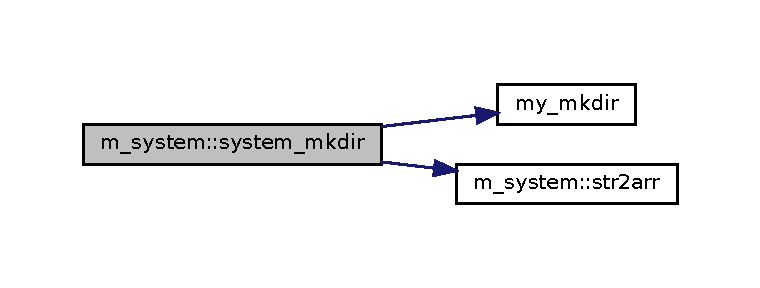
\includegraphics[width=350pt]{namespacem__system_a084d644c236d22af2cc75c6e48fd6e96_cgraph}
\end{center}
\end{figure}
\mbox{\Hypertarget{namespacem__system_ab2d95258ee26b85a0283538880775475}\label{namespacem__system_ab2d95258ee26b85a0283538880775475}} 
\index{m\+\_\+system@{m\+\_\+system}!system\+\_\+mkfifo@{system\+\_\+mkfifo}}
\index{system\+\_\+mkfifo@{system\+\_\+mkfifo}!m\+\_\+system@{m\+\_\+system}}
\subsubsection{\texorpdfstring{system\+\_\+mkfifo()}{system\_mkfifo()}}
{\footnotesize\ttfamily integer function, public m\+\_\+system\+::system\+\_\+mkfifo (\begin{DoxyParamCaption}\item[{character(len=$\ast$), intent(in)}]{pathname,  }\item[{integer, intent(in)}]{mode }\end{DoxyParamCaption})}



\subsubsection*{N\+A\+ME}

system\+\_\+mkfifo(3f) -\/ \mbox{[}M\+\_\+system\mbox{]} make a F\+I\+FO special file relative to directory file descriptor (L\+I\+C\+E\+N\+SE\+:PD) \subsubsection*{S\+Y\+N\+O\+P\+S\+IS}

function system\+\_\+mkfifo(pathname,mode) result(ierr)

character(len=$\ast$),intent(in) \+:\+: pathname integer,intent(in) \+:\+: mode integer \+:\+: ierr

\subsubsection*{D\+E\+S\+C\+R\+I\+P\+T\+I\+ON}

A regular pipe can only connect two related processes. It is created by a process and will vanish when the last process closes it.

A named pipe, also called a F\+I\+FO for its behavior, can be used to connect two unrelated processes and exists independently of the processes; meaning it can exist even if no one is using it. A F\+I\+FO is created using the mkfifo() library function.

The mkfifo() function creates a new F\+I\+FO special file named by the pathname.

The file permission bits of the new F\+I\+FO are initialized from mode.

The file permission bits of the mode argument are modified by the process\textquotesingle{} file creation mask.

When bits in mode other than the file permission bits are set, the effect is implementation-\/defined.

If path names a symbolic link, mkfifo() shall fail and set errno to \mbox{[}E\+E\+X\+I\+ST\mbox{]}.

The F\+I\+FO\textquotesingle{}s user ID will be set to the process\textquotesingle{} effective user ID.

The F\+I\+FO\textquotesingle{}s group ID shall be set to the group ID of the parent directory or to the effective group ID of the process.

Implementations shall provide a way to initialize the F\+I\+FO\textquotesingle{}s group ID to the group ID of the parent directory.

Implementations may, but need not, provide an implementation-\/defined way to initialize the F\+I\+FO\textquotesingle{}s group ID to the effective group ID of the calling process.

Upon successful completion, mkfifo() shall mark for update the last data access, last data modification, and last file status change timestamps of the file.

Also, the last data modification and last file status change timestamps of the directory that contains the new entry shall be marked for update.

Predefined variables are typically used to set permission modes.

You can bytewise-\/\+OR together these variables to to create the most common permissions mode\+:

User\+: R\+\_\+\+U\+SR (read), W\+\_\+\+U\+SR (write), X\+\_\+\+U\+S\+R(execute) Group\+: R\+\_\+\+G\+RP (read), W\+\_\+\+G\+RP (write), X\+\_\+\+G\+R\+P(execute) Others\+: R\+\_\+\+O\+TH (read), W\+\_\+\+O\+TH (write), X\+\_\+\+O\+T\+H(execute)

Additionally, some shortcuts are provided (basically a bitwise-\/\+OR combination of the above)\+:

Read + Write + Execute\+: R\+W\+X\+\_\+U (User), R\+W\+X\+\_\+G (Group), R\+W\+X\+\_\+O (Others) D\+E\+F\+F\+I\+L\+E\+M\+O\+DE\+: Equivalent of 0666 =rw-\/rw-\/rw-\/ A\+C\+C\+E\+S\+S\+P\+E\+R\+MS\+: Equivalent of 0777 = rwxrwxrwx

Therefore, to give only the user rwx (read+write+execute) rights whereas group members and others may not do anything, you can use any of the following mkfifo() calls equivalently\+:

ierr= mkfifo(\char`\"{}myfile\char`\"{}, I\+A\+N\+Y(\mbox{[}\+R\+\_\+\+U\+S\+R, W\+\_\+\+U\+S\+R, X\+\_\+\+U\+S\+R\mbox{]})); ierr= mkfifo(\char`\"{}myfile\char`\"{}, R\+W\+X\+\_\+U);

In order to give anyone any rights (mode 0777 = rwxrwxrwx), you can use any of the following calls equivalently\+:

ierr= mkfifo(\char`\"{}myfile\char`\"{},I\+A\+N\+Y(\mbox{[}\+R\+\_\+\+U\+S\+R,\+W\+\_\+\+U\+S\+R,\+X\+\_\+\+U\+S\+R,\+R\+\_\+\+G\+R\+P,\+W\+\_\+\+G\+R\+P,\+X\+\_\+\+G\+R\+P,\+R\+\_\+\+O\+T\+H,\+W\+\_\+\+O\+T\+H,\+X\+\_\+\+O\+T\+H\mbox{]})); ierr= mkfifo(\char`\"{}myfile\char`\"{},I\+A\+N\+Y(\mbox{[}\+R\+W\+X\+\_\+\+U,\+R\+W\+X\+\_\+\+G,\+R\+W\+X\+\_\+\+O\mbox{]})); ierr= mkfifo(\char`\"{}myfile\char`\"{},A\+C\+C\+E\+S\+S\+P\+E\+R\+MS); \subsubsection*{R\+E\+T\+U\+RN V\+A\+L\+UE}

Upon successful completion, return 0. Otherwise, return -\/1 and set errno to indicate the error. If -\/1 is returned, no F\+I\+FO is created.

\subsubsection*{E\+X\+A\+M\+P\+L\+ES}

The following example shows how to create a F\+I\+FO file named /home/cnd/mod\+\_\+done, with read/write permissions for owner, and with read permissions for group and others.

program demo\+\_\+system\+\_\+mkfifo use M\+\_\+system, only \+: system\+\_\+mkfifo, system\+\_\+perror use M\+\_\+system, only \+: R\+\_\+\+G\+RP,R\+\_\+\+O\+TH,R\+\_\+\+U\+SR,R\+W\+X\+\_\+G,R\+W\+X\+\_\+O use M\+\_\+system, only \+: R\+W\+X\+\_\+U,W\+\_\+\+G\+RP,W\+\_\+\+O\+TH,W\+\_\+\+U\+SR,X\+\_\+\+G\+RP,X\+\_\+\+O\+TH,X\+\_\+\+U\+SR use M\+\_\+system, only \+: D\+E\+F\+F\+I\+L\+E\+M\+O\+DE, A\+C\+C\+E\+S\+S\+P\+E\+R\+MS implicit none integer \+:\+: status status = system\+\_\+mkfifo(\char`\"{}/tmp/buffer\char`\"{}, I\+A\+N\+Y(\mbox{[}\+W\+\_\+\+U\+S\+R, R\+\_\+\+U\+S\+R, R\+\_\+\+G\+R\+P, R\+\_\+\+O\+T\+H\mbox{]})) if(status.\+ne.\+0)then call system\+\_\+perror(\textquotesingle{}{\itshape mkfifo} error\+:\textquotesingle{}) endif end program demo\+\_\+system\+\_\+mkfifo

Now some other process (or this one) can read from /tmp/buffer while this program is running or after, consuming the data as it is read.

\subsubsection*{A\+U\+T\+H\+OR}

John S. Urban \subsubsection*{L\+I\+C\+E\+N\+SE}

Public Domain 

References str2arr().

Here is the call graph for this function\+:
\nopagebreak
\begin{figure}[H]
\begin{center}
\leavevmode
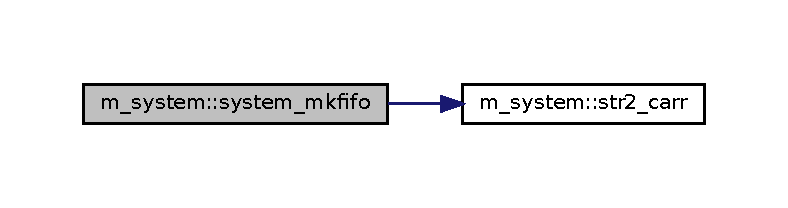
\includegraphics[width=350pt]{namespacem__system_ab2d95258ee26b85a0283538880775475_cgraph}
\end{center}
\end{figure}
\mbox{\Hypertarget{namespacem__system_a622cc67c03e8cdea1d4c2430bb36081b}\label{namespacem__system_a622cc67c03e8cdea1d4c2430bb36081b}} 
\index{m\+\_\+system@{m\+\_\+system}!system\+\_\+opendir@{system\+\_\+opendir}}
\index{system\+\_\+opendir@{system\+\_\+opendir}!m\+\_\+system@{m\+\_\+system}}
\subsubsection{\texorpdfstring{system\+\_\+opendir()}{system\_opendir()}}
{\footnotesize\ttfamily subroutine, public m\+\_\+system\+::system\+\_\+opendir (\begin{DoxyParamCaption}\item[{character(len=$\ast$), intent(in)}]{dirname,  }\item[{type(c\+\_\+ptr)}]{dir,  }\item[{integer, intent(out)}]{ierr }\end{DoxyParamCaption})}



\subsubsection*{N\+A\+ME}

system\+\_\+opendir(3f) -\/ \mbox{[}M\+\_\+system\mbox{]} open directory stream by calling opendir(3c) (L\+I\+C\+E\+N\+SE\+:PD) \subsubsection*{S\+Y\+N\+O\+P\+S\+IS}

subroutine system\+\_\+opendir(dirname,dir,ierr)

character(len=$\ast$), intent(in) \+:\+: dirname type(c\+\_\+ptr) \+:\+: dir integer,intent(out) \+:\+: ierr

\subsubsection*{D\+E\+S\+C\+R\+I\+P\+T\+I\+ON}

The system\+\_\+opendir(3f) procedure opens a directory stream corresponding to the directory named by the dirname argument. The directory stream is positioned at the first entry.

\subsubsection*{R\+E\+T\+U\+RN V\+A\+L\+UE}

Upon successful completion, a pointer to a C dir type is returned. Otherwise, these functions shall return a null pointer and set I\+E\+RR to indicate the error.

\subsubsection*{E\+R\+R\+O\+RS}

\begin{DoxyVerb}    An error corresponds to a condition described in opendir(3c):

    EACCES    Search permission is denied for the component of the
              path prefix of dirname or read permission is denied
              for dirname.

    ELOOP     A loop exists in symbolic links encountered during
              resolution of the dirname argument.

    ENAMETOOLONG  The length of a component of a pathname is longer than {NAME_MAX}.

    ENOENT        A component of dirname does not name an existing directory or dirname is an empty string.

    ENOTDIR       A component of dirname names an existing file that is neither a directory nor a symbolic link to a directory.

    ELOOP         More than {SYMLOOP_MAX} symbolic links were encountered during resolution of the dirname argument.

    EMFILE        All file descriptors available to the process are currently open.

    ENAMETOOLONG  The length of a pathname exceeds {PATH_MAX},
                  or pathname resolution of a symbolic link produced an intermediate
                  result with a length that exceeds {PATH_MAX}.

    ENFILE        Too many files are currently open in the system.
\end{DoxyVerb}


\subsubsection*{A\+P\+P\+L\+I\+C\+A\+T\+I\+ON U\+S\+A\+GE}

The opendir() function should be used in conjunction with readdir(), closedir(), and rewinddir() to examine the contents of the directory (see the E\+X\+A\+M\+P\+L\+ES section in readdir()). This method is recommended for portability. \subsubsection*{O\+P\+T\+I\+O\+NS}

dirname name of directory to open a directory stream for \subsubsection*{R\+E\+T\+U\+R\+NS}

dir pointer to directory stream. If an error occurred, it will not be associated. ierr 0 indicates no error occurred \subsubsection*{E\+X\+A\+M\+P\+LE}

Sample program\+:

program demo\+\_\+system\+\_\+opendir use M\+\_\+system, only \+: system\+\_\+opendir,system\+\_\+readdir use M\+\_\+system, only \+: system\+\_\+closedir use iso\+\_\+c\+\_\+binding implicit none type(c\+\_\+ptr) \+:\+: dir character(len=\+:),allocatable \+:\+: filename integer \+:\+: ierr !--- open directory stream to read from call system\+\_\+opendir(\textquotesingle{}.\textquotesingle{},dir,ierr) if(ierr.\+eq.\+0)then !--- read directory stream do call system\+\_\+readdir(dir,filename,ierr) if(filename.\+eq.\textquotesingle{} \textquotesingle{})exit write($\ast$,$\ast$)filename enddo endif !--- close directory stream call system\+\_\+closedir(dir,ierr) end program demo\+\_\+system\+\_\+opendir \subsubsection*{A\+U\+T\+H\+OR}

John S. Urban \subsubsection*{L\+I\+C\+E\+N\+SE}

Public Domain 

References str2arr().

Here is the call graph for this function\+:
\nopagebreak
\begin{figure}[H]
\begin{center}
\leavevmode
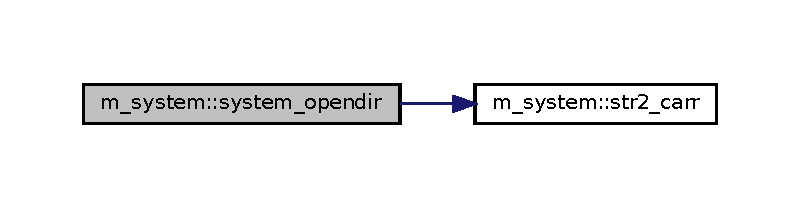
\includegraphics[width=350pt]{namespacem__system_a622cc67c03e8cdea1d4c2430bb36081b_cgraph}
\end{center}
\end{figure}
\mbox{\Hypertarget{namespacem__system_ae8f39e1d4e420396319105e4e81f92b5}\label{namespacem__system_ae8f39e1d4e420396319105e4e81f92b5}} 
\index{m\+\_\+system@{m\+\_\+system}!system\+\_\+perm@{system\+\_\+perm}}
\index{system\+\_\+perm@{system\+\_\+perm}!m\+\_\+system@{m\+\_\+system}}
\subsubsection{\texorpdfstring{system\+\_\+perm()}{system\_perm()}}
{\footnotesize\ttfamily character(len=\+:) function, allocatable, public m\+\_\+system\+::system\+\_\+perm (\begin{DoxyParamCaption}\item[{class($\ast$), intent(in)}]{mode }\end{DoxyParamCaption})}



\subsubsection*{N\+A\+ME}

system\+\_\+perm(3f) -\/ \mbox{[}M\+\_\+system\mbox{]} get file type and permission as a string (L\+I\+C\+E\+N\+SE\+:PD) 

\subsubsection*{S\+Y\+N\+O\+P\+S\+IS}

function system\+\_\+perm(mode) result (perms)

integer(kind=int64),intent(in) \+:\+: M\+O\+DE character(len=\+:),allocatable \+:\+: P\+E\+R\+MS

\subsubsection*{D\+E\+S\+C\+R\+I\+P\+T\+I\+ON}

\begin{DoxyVerb}The system_perm(3f) function returns a string containing the type
and permission of a file implied by the value of the mode value.
\end{DoxyVerb}


\subsubsection*{R\+E\+T\+U\+RN V\+A\+L\+UE}

P\+E\+R\+MS returns the permission string in a format similar to that used by Unix commands such as ls(1).

\subsubsection*{E\+X\+A\+M\+P\+LE}

Sample program\+:

program demo\+\_\+system\+\_\+perm use M\+\_\+system, only \+: system\+\_\+perm, system\+\_\+stat use,intrinsic \+:\+: iso\+\_\+fortran\+\_\+env, only \+: int64 implicit none character(len=4096) \+:\+: string integer(kind=int64) \+:\+: values(13) integer \+:\+: ierr character(len=\+:),allocatable \+:\+: perms values=0 call get\+\_\+command\+\_\+argument(1, string) ! get pathname from command line call system\+\_\+stat(string,values,ierr) ! get pathname information if(ierr.\+eq.\+0)then perms=system\+\_\+perm(values(3)) ! convert permit mode to a string ! print permits as a string, decimal value, and octal value write($\ast$,\textquotesingle{}(\char`\"{}for \char`\"{},a,\char`\"{} permits\mbox{[}\char`\"{},a,\char`\"{}\mbox{]}\char`\"{},1x,i0,1x,o0)\textquotesingle{}) \& trim(string),perms,values(3),values(3) endif end program demo\+\_\+system\+\_\+perm

Results\+:

demo\+\_\+system\+\_\+perm /tmp

for /tmp permits\mbox{[}drwxrwxrwx --S\mbox{]} 17407 41777

\subsubsection*{A\+U\+T\+H\+OR}

John S. Urban \subsubsection*{L\+I\+C\+E\+N\+SE}

Public Domain 

References anyinteger\+\_\+to\+\_\+64bit(), and c2f\+\_\+string().

Here is the call graph for this function\+:
\nopagebreak
\begin{figure}[H]
\begin{center}
\leavevmode
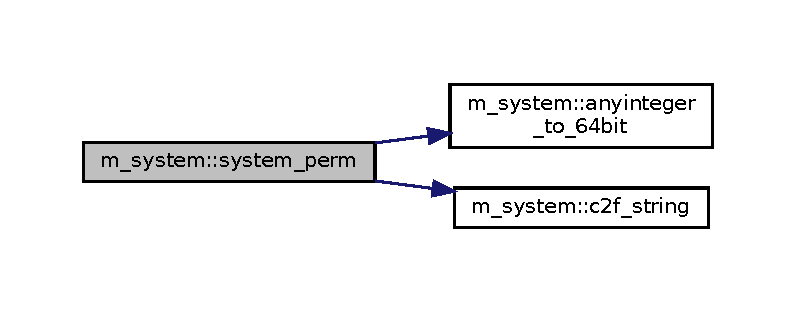
\includegraphics[width=350pt]{namespacem__system_ae8f39e1d4e420396319105e4e81f92b5_cgraph}
\end{center}
\end{figure}
\mbox{\Hypertarget{namespacem__system_afae451a1fc5432274dc1f75a364051b4}\label{namespacem__system_afae451a1fc5432274dc1f75a364051b4}} 
\index{m\+\_\+system@{m\+\_\+system}!system\+\_\+perror@{system\+\_\+perror}}
\index{system\+\_\+perror@{system\+\_\+perror}!m\+\_\+system@{m\+\_\+system}}
\subsubsection{\texorpdfstring{system\+\_\+perror()}{system\_perror()}}
{\footnotesize\ttfamily subroutine, public m\+\_\+system\+::system\+\_\+perror (\begin{DoxyParamCaption}\item[{character(len=$\ast$), intent(in)}]{prefix }\end{DoxyParamCaption})}



\subsubsection*{N\+A\+ME}

perror(3f) -\/ \mbox{[}M\+\_\+system\mbox{]} print error message for last C error on stderr (L\+I\+C\+E\+N\+SE\+:PD) \subsubsection*{S\+Y\+N\+O\+P\+S\+IS}

subroutine system\+\_\+perror(prefix)

character(len=$\ast$),intent(in) \+:\+: prefix

\subsubsection*{D\+E\+S\+C\+R\+I\+P\+T\+I\+ON}

Use system\+\_\+perror(3f) to print an error message on stderr corresponding to the current value of the C global variable errno. Unless you use N\+U\+LL as the argument prefix, the error message will begin with the prefix string, followed by a colon and a space (\+:). The remainder of the error message produced is one of the strings described for strerror(3c).

\subsubsection*{E\+X\+A\+M\+P\+LE}

Sample program\+:

program demo\+\_\+system\+\_\+perror use M\+\_\+system, only \+: system\+\_\+perror,system\+\_\+rmdir implicit none character(len=\+:),allocatable \+:\+: D\+I\+R\+N\+A\+ME D\+I\+R\+N\+A\+ME=\textquotesingle{}/\+N\+O\+T/\+T\+H\+E\+R\+E/\+O\+R/\+A\+N\+Y\+W\+H\+E\+RE\textquotesingle{} ! generate an error with a routine that supports errno and perror(3c) if(system\+\_\+rmdir(\+D\+I\+R\+N\+A\+M\+E).ne.\+0)then call system\+\_\+perror(\textquotesingle{}{\itshape demo\+\_\+system\+\_\+perror}\+:\textquotesingle{}//\+D\+I\+R\+N\+A\+ME) endif write($\ast$,\textquotesingle{}(a)\textquotesingle{})\char`\"{}\+That\textquotesingle{}s all Folks!\char`\"{} end program demo\+\_\+system\+\_\+perror

Expected results\+:

{\itshape demo\+\_\+system\+\_\+perror}\+:/\+N\+O\+T/\+T\+H\+E\+R\+E/\+O\+R/\+A\+N\+Y\+W\+H\+E\+RE\+: No such file or directory That\textquotesingle{}s all Folks! 

References str2arr().

Here is the call graph for this function\+:
\nopagebreak
\begin{figure}[H]
\begin{center}
\leavevmode
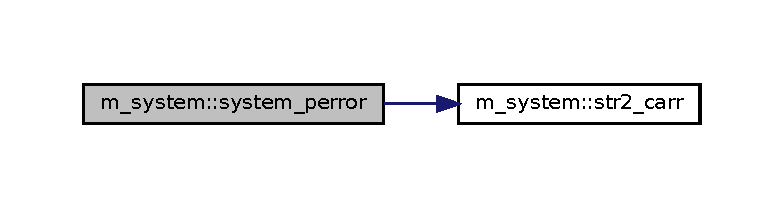
\includegraphics[width=350pt]{namespacem__system_afae451a1fc5432274dc1f75a364051b4_cgraph}
\end{center}
\end{figure}
\mbox{\Hypertarget{namespacem__system_af0c9df8e59cac9cd617cd1e20448ea7d}\label{namespacem__system_af0c9df8e59cac9cd617cd1e20448ea7d}} 
\index{m\+\_\+system@{m\+\_\+system}!system\+\_\+putenv@{system\+\_\+putenv}}
\index{system\+\_\+putenv@{system\+\_\+putenv}!m\+\_\+system@{m\+\_\+system}}
\subsubsection{\texorpdfstring{system\+\_\+putenv()}{system\_putenv()}}
{\footnotesize\ttfamily subroutine, public m\+\_\+system\+::system\+\_\+putenv (\begin{DoxyParamCaption}\item[{character(len=$\ast$), intent(in)}]{string,  }\item[{integer, intent(out), optional}]{err }\end{DoxyParamCaption})}



\subsubsection*{N\+A\+ME}

system\+\_\+putenv(3f) -\/ \mbox{[}M\+\_\+system\+:E\+N\+V\+I\+R\+O\+N\+M\+E\+NT\mbox{]} set environment variable from Fortran by calling putenv(3c) (L\+I\+C\+E\+N\+SE\+:PD) 

\subsubsection*{S\+Y\+N\+O\+P\+S\+IS}

\begin{DoxyVerb}subroutine system_putenv(string, err)

 character(len=*),intent(in)    :: string
 integer, optional, intent(out) :: err
\end{DoxyVerb}


\subsubsection*{D\+E\+S\+C\+R\+I\+P\+T\+I\+ON}

The \mbox{\hyperlink{namespacem__system_af0c9df8e59cac9cd617cd1e20448ea7d}{system\+\_\+putenv()}} function adds or changes the value of environment variables.

\subsubsection*{O\+P\+T\+I\+O\+NS}

string string of format \char`\"{}\+N\+A\+M\+E=value\char`\"{}. If name does not already exist in the environment, then string is added to the environment. If name does exist, then the value of name in the environment is changed to value. The string passed to putenv(3c) becomes part of the environment, so this routine creates a string each time it is called that increases the amount of memory the program uses. err The \mbox{\hyperlink{namespacem__system_af0c9df8e59cac9cd617cd1e20448ea7d}{system\+\_\+putenv()}} function returns zero on success, or nonzero if an error occurs. A non-\/zero error usually indicates sufficient memory does not exist to store the variable.

\subsubsection*{E\+X\+A\+M\+P\+LE}

Sample setting an environment variable from Fortran\+:

program demo\+\_\+system\+\_\+putenv use M\+\_\+system, only \+: system\+\_\+putenv use iso\+\_\+c\+\_\+binding implicit none integer \+:\+: ierr ! write($\ast$,\textquotesingle{}(a)\textquotesingle{})\textquotesingle{}no environment variables containing \char`\"{}\+G\+R\+U\char`\"{}\+:\textquotesingle{} call execute\+\_\+command\+\_\+line(\textquotesingle{}env$\vert$grep G\+RU\textquotesingle{}) ! call system\+\_\+putenv(\textquotesingle{}G\+RU=this is the value\textquotesingle{},ierr) write($\ast$,\textquotesingle{}(a,i0)\textquotesingle{})\textquotesingle{}now \char`\"{}\+G\+R\+U\char`\"{} should be defined\+: \textquotesingle{},ierr call execute\+\_\+command\+\_\+line(\textquotesingle{}env$\vert$grep G\+RU\textquotesingle{}) ! call system\+\_\+putenv(\textquotesingle{}G\+R\+U2=this is the second value\textquotesingle{},ierr) write($\ast$,\textquotesingle{}(a,i0)\textquotesingle{})\textquotesingle{}now \char`\"{}\+G\+R\+U\char`\"{} and \char`\"{}\+G\+R\+U2\char`\"{} should be defined\+: \textquotesingle{},ierr call execute\+\_\+command\+\_\+line(\textquotesingle{}env$\vert$grep G\+RU\textquotesingle{}) ! call system\+\_\+putenv(\textquotesingle{}G\+R\+U2\textquotesingle{},ierr) call system\+\_\+putenv(\textquotesingle{}G\+RU\textquotesingle{},ierr) write($\ast$,\textquotesingle{}(a,i0)\textquotesingle{})\textquotesingle{}should be gone, varies with different putenv(3c)\+: \textquotesingle{},ierr call execute\+\_\+command\+\_\+line(\textquotesingle{}env$\vert$grep G\+RU\textquotesingle{}) write($\ast$,\textquotesingle{}(a)\textquotesingle{})\textquotesingle{}system\+\_\+unsetenv(3f) is a better way to remove variables\textquotesingle{} ! end program demo\+\_\+system\+\_\+putenv

Results\+:

no environment variables containing \char`\"{}\+G\+R\+U\char`\"{}\+: now \char`\"{}\+G\+R\+U\char`\"{} should be defined\+: 0 G\+RU=this is the value now \char`\"{}\+G\+R\+U\char`\"{} and \char`\"{}\+G\+R\+U2\char`\"{} should be defined\+: 0 G\+R\+U2=this is the second value G\+RU=this is the value should be gone, varies with different putenv(3c)\+: 0 system\+\_\+unsetenv(3f) is a better way to remove variables

\subsubsection*{A\+U\+T\+H\+OR}

John S. Urban \subsubsection*{L\+I\+C\+E\+N\+SE}

Public Domain \mbox{\Hypertarget{namespacem__system_a983df5b2d7cb5842d69c4a31829403e0}\label{namespacem__system_a983df5b2d7cb5842d69c4a31829403e0}} 
\index{m\+\_\+system@{m\+\_\+system}!system\+\_\+readdir@{system\+\_\+readdir}}
\index{system\+\_\+readdir@{system\+\_\+readdir}!m\+\_\+system@{m\+\_\+system}}
\subsubsection{\texorpdfstring{system\+\_\+readdir()}{system\_readdir()}}
{\footnotesize\ttfamily subroutine, public m\+\_\+system\+::system\+\_\+readdir (\begin{DoxyParamCaption}\item[{type(c\+\_\+ptr), value}]{dir,  }\item[{character(len=\+:), intent(out), allocatable}]{filename,  }\item[{integer, intent(out)}]{ierr }\end{DoxyParamCaption})}



\subsubsection*{N\+A\+ME}

system\+\_\+readdir(3f) -\/ \mbox{[}M\+\_\+system\mbox{]} read a directory using readdir(3c) (L\+I\+C\+E\+N\+SE\+:PD) \subsubsection*{S\+Y\+N\+O\+P\+S\+IS}

subroutine system\+\_\+readdir(dir,filename,ierr)

type(c\+\_\+ptr),value \+:\+: dir character(len=\+:),intent(out),allocatable \+:\+: filename integer,intent(out) \+:\+: ierr

\subsubsection*{D\+E\+S\+C\+R\+I\+P\+T\+I\+ON}

\begin{DoxyVerb}system_readdir(3f) returns the name of the directory entry at the
current position in the directory stream specified by the argument
DIR, and positions the directory stream at the next entry. It returns
a null name upon reaching the end of the directory stream.
\end{DoxyVerb}


\subsubsection*{O\+P\+T\+I\+O\+NS}

\begin{DoxyVerb}DIR       A pointer to the directory opened by system_opendir(3f).
\end{DoxyVerb}


\subsubsection*{R\+E\+T\+U\+R\+NS}

\begin{DoxyVerb}FILENAME  the name of the directory entry at the current position in
          the directory stream specified by the argument DIR, and
          positions the directory stream at the next entry.

          The readdir() function does not return directory entries
          containing empty names. If entries for dot or dot-dot exist,
          one entry is returned for dot and one entry is returned
          for dot-dot.

          The entry is marked for update of the last data access
          timestamp each time it is read.

          reaching the end of the directory stream, the name is a blank name.

IERR      If IERR is set to non-zero on return, an error occurred.
\end{DoxyVerb}


\subsubsection*{E\+X\+A\+M\+P\+LE}

Sample program\+:

program demo\+\_\+system\+\_\+readdir use M\+\_\+system, only \+: system\+\_\+opendir,system\+\_\+readdir use M\+\_\+system, only \+: system\+\_\+rewinddir,system\+\_\+closedir use iso\+\_\+c\+\_\+binding implicit none

type(c\+\_\+ptr) \+:\+: dir character(len=\+:),allocatable \+:\+: filename integer \+:\+: i, ierr !--- open directory stream to read from call system\+\_\+opendir(\textquotesingle{}.\textquotesingle{},dir,ierr) if(ierr.\+eq.\+0)then !--- read directory stream twice do i=1,2 write($\ast$,\textquotesingle{}(a,i0)\textquotesingle{})\textquotesingle{}P\+A\+SS \textquotesingle{},i do call system\+\_\+readdir(dir,filename,ierr) if(filename.\+eq.\textquotesingle{} \textquotesingle{})exit write($\ast$,$\ast$)filename enddo call system\+\_\+rewinddir(dir) enddo endif !--- close directory stream call system\+\_\+closedir(dir,ierr)

end program demo\+\_\+system\+\_\+readdir

\subsubsection*{A\+U\+T\+H\+OR}

John S. Urban \subsubsection*{L\+I\+C\+E\+N\+SE}

Public Domain 

References arr2str().

Here is the call graph for this function\+:
\nopagebreak
\begin{figure}[H]
\begin{center}
\leavevmode
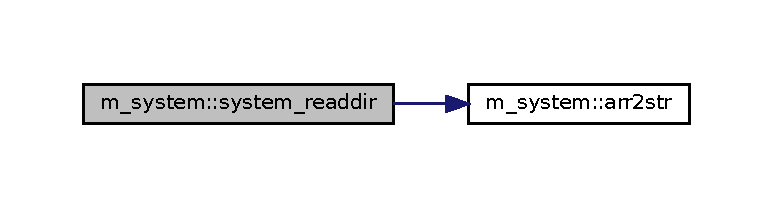
\includegraphics[width=350pt]{namespacem__system_a983df5b2d7cb5842d69c4a31829403e0_cgraph}
\end{center}
\end{figure}
\mbox{\Hypertarget{namespacem__system_ae0e43010a82a6a25402568ccb326322d}\label{namespacem__system_ae0e43010a82a6a25402568ccb326322d}} 
\index{m\+\_\+system@{m\+\_\+system}!system\+\_\+readenv@{system\+\_\+readenv}}
\index{system\+\_\+readenv@{system\+\_\+readenv}!m\+\_\+system@{m\+\_\+system}}
\subsubsection{\texorpdfstring{system\+\_\+readenv()}{system\_readenv()}}
{\footnotesize\ttfamily character(len=\+:) function, allocatable, public m\+\_\+system\+::system\+\_\+readenv (\begin{DoxyParamCaption}{ }\end{DoxyParamCaption})}



\subsubsection*{N\+A\+ME}

system\+\_\+readenv(3f) -\/ \mbox{[}M\+\_\+system\+:E\+N\+V\+I\+R\+O\+N\+M\+E\+NT\mbox{]} step thru and read environment table (L\+I\+C\+E\+N\+SE\+:PD) \subsubsection*{S\+Y\+N\+O\+P\+S\+IS}

function \mbox{\hyperlink{namespacem__system_ae0e43010a82a6a25402568ccb326322d}{system\+\_\+readenv()}} result(string)

character(len=\+:),allocatable \+:\+: string \subsubsection*{D\+E\+S\+C\+R\+I\+P\+T\+I\+ON}

A simple interface allows reading the environment variable table of the process. Call system\+\_\+initenv(3f) to initialize reading the environment table, then call system\+\_\+readenv(3f) can be called until a blank line is returned. If more than one thread reads the environment or the environment is changed while being read the results are undefined. \subsubsection*{O\+P\+T\+I\+O\+NS}

string the string returned from the environment of the form \char`\"{}\+N\+A\+M\+E=\+V\+A\+L\+U\+E\char`\"{}

\subsubsection*{E\+X\+A\+M\+P\+LE}

Sample program\+:

program demo\+\_\+system\+\_\+readenv use M\+\_\+system, only \+: \mbox{\hyperlink{interfacem__system_1_1system__initenv}{system\+\_\+initenv}}, system\+\_\+readenv character(len=\+:),allocatable \+:\+: string call system\+\_\+initenv() do string=\mbox{\hyperlink{namespacem__system_ae0e43010a82a6a25402568ccb326322d}{system\+\_\+readenv()}} if(string.\+eq.\textquotesingle{}\textquotesingle{})then exit else write($\ast$,\textquotesingle{}(a)\textquotesingle{})string endif enddo end program demo\+\_\+system\+\_\+readenv

Sample results\+:

U\+S\+E\+R\+D\+O\+M\+A\+I\+N\+\_\+\+R\+O\+A\+M\+I\+N\+G\+P\+R\+O\+F\+I\+LE=buzz H\+O\+M\+E\+P\+A\+TH= A\+P\+P\+D\+A\+TA=C\+: M\+A\+N\+P\+A\+TH=/home/urbanjs/\+V600/\+L\+I\+B\+R\+A\+R\+Y/lib\+G\+P\+F/download/tmp/man\+:/home/urbanjs/\+V600/doc/man\+:\+:\+: D\+I\+S\+P\+L\+A\+Y\+N\+UM=0 Program\+W6432=C\+: Files H\+O\+S\+T\+N\+A\+ME=buzz X\+K\+E\+Y\+S\+Y\+M\+DB=/usr/share/\+X11/\+X\+Keysym\+DB P\+U\+B\+L\+I\+S\+H\+\_\+\+C\+MD= Online\+Services=Online Services \+: \+: \+: \subsubsection*{A\+U\+T\+H\+OR}

John S. Urban \subsubsection*{L\+I\+C\+E\+N\+SE}

Public Domain 

References arr2str().

Here is the call graph for this function\+:
\nopagebreak
\begin{figure}[H]
\begin{center}
\leavevmode
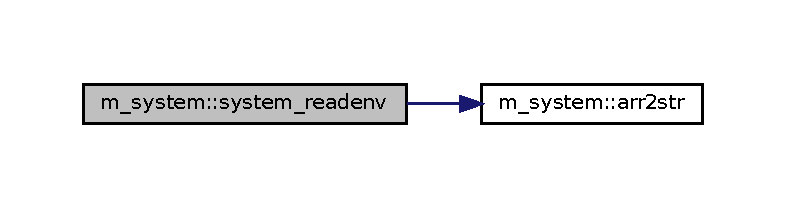
\includegraphics[width=350pt]{namespacem__system_ae0e43010a82a6a25402568ccb326322d_cgraph}
\end{center}
\end{figure}
Here is the caller graph for this function\+:
\nopagebreak
\begin{figure}[H]
\begin{center}
\leavevmode
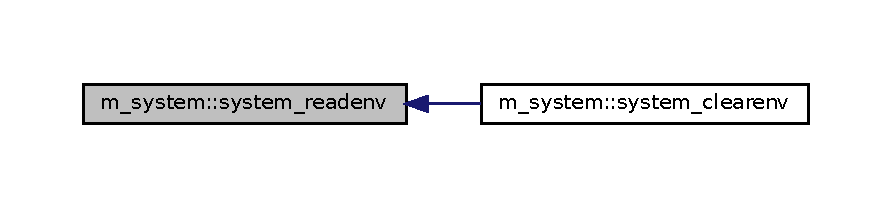
\includegraphics[width=350pt]{namespacem__system_ae0e43010a82a6a25402568ccb326322d_icgraph}
\end{center}
\end{figure}
\mbox{\Hypertarget{namespacem__system_a70bbfa0a0be084b9717cbc04408041fc}\label{namespacem__system_a70bbfa0a0be084b9717cbc04408041fc}} 
\index{m\+\_\+system@{m\+\_\+system}!system\+\_\+realpath@{system\+\_\+realpath}}
\index{system\+\_\+realpath@{system\+\_\+realpath}!m\+\_\+system@{m\+\_\+system}}
\subsubsection{\texorpdfstring{system\+\_\+realpath()}{system\_realpath()}}
{\footnotesize\ttfamily character(len=\+:) function, allocatable, public m\+\_\+system\+::system\+\_\+realpath (\begin{DoxyParamCaption}\item[{character(len=$\ast$), intent(in)}]{input }\end{DoxyParamCaption})}



\subsubsection*{N\+A\+ME}

system\+\_\+realpath(3f) -\/ \mbox{[}M\+\_\+system\mbox{]} call realpath(3c) to resolve a pathname (L\+I\+C\+E\+N\+SE\+:PD) \subsubsection*{S\+Y\+N\+O\+P\+S\+IS}

function system\+\_\+realpath(input) result(output)

character(len=$\ast$),intent(in) \+:\+: input character(len=\+:),allocatable \+:\+: output \subsubsection*{D\+E\+S\+C\+R\+I\+P\+T\+I\+ON}

system\+\_\+realpath(3f) calls the C routine realpath(3c) to obtain the absolute pathname of given path \subsubsection*{O\+P\+T\+I\+O\+NS}

\begin{DoxyVerb}    INPUT     pathname to resolve
\end{DoxyVerb}


\subsubsection*{R\+E\+T\+U\+RN V\+A\+L\+UE}

O\+U\+T\+P\+UT The absolute pathname of the given input pathname. The pathname shall contain no components that are dot or dot-\/dot, or are symbolic links. It is equal to the N\+U\+LL character if an error occurred.

\subsubsection*{E\+X\+A\+M\+P\+LE}

Sample program\+:

program demo\+\_\+system\+\_\+realpath use M\+\_\+system, only \+: system\+\_\+realpath, system\+\_\+perror implicit none ! resolve each pathname given on command line character(len=\+:),allocatable \+:\+: pathi,patho integer \+:\+: i integer \+:\+: filename\+\_\+length do i = 1, command\+\_\+argument\+\_\+count() ! get pathname from command line arguments call get\+\_\+command\+\_\+argument (i , length=filename\+\_\+length) allocate(character(len=filename\+\_\+length) \+:\+: pathi) call get\+\_\+command\+\_\+argument (i , value=pathi) ! ! resolve each pathname patho=system\+\_\+realpath(pathi) if(patho.\+ne.\+char(0))then write($\ast$,$\ast$)trim(pathi),\textquotesingle{}=$>$\textquotesingle{},trim(patho) else call system\+\_\+perror(\textquotesingle{}{\itshape system\+\_\+realpath} error for pathname \textquotesingle{}//trim(pathi)//\textquotesingle{}\+:\textquotesingle{}) write($\ast$,$\ast$)trim(pathi),\textquotesingle{}=$>$\textquotesingle{},trim(patho) endif deallocate(pathi) enddo ! if there were no pathnames give resolve the pathname \char`\"{}.\char`\"{} if(i.\+eq.\+1)then patho=system\+\_\+realpath(\textquotesingle{}.\textquotesingle{}) write($\ast$,$\ast$)\textquotesingle{}.=$>$\textquotesingle{},trim(patho) endif end program demo\+\_\+system\+\_\+realpath

Example usage\+:

demo\+\_\+system\+\_\+realpath .=$>$/home/urbanjs/\+V600

cd /usr/share/man demo\+\_\+system\+\_\+realpath . .. Not\+There .=$>$/usr/share/man ..=$>$/usr/share {\itshape system\+\_\+realpath} error for pathname Not\+There\+:\+: No such file or directory Not\+There=$>$Not\+There 

References c2f\+\_\+string(), and str2arr().

Here is the call graph for this function\+:
\nopagebreak
\begin{figure}[H]
\begin{center}
\leavevmode
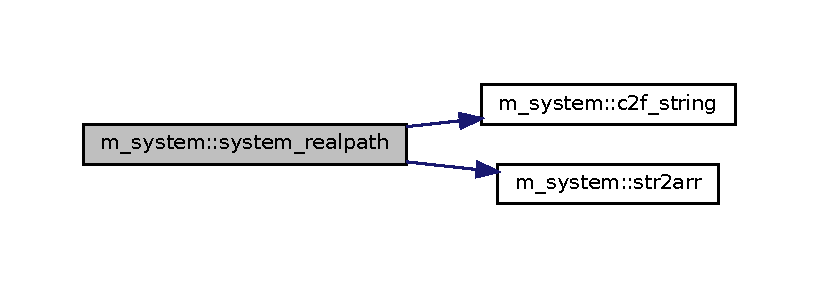
\includegraphics[width=350pt]{namespacem__system_a70bbfa0a0be084b9717cbc04408041fc_cgraph}
\end{center}
\end{figure}
\mbox{\Hypertarget{namespacem__system_a730ae64294e3cd73bde8f0c63cdf9972}\label{namespacem__system_a730ae64294e3cd73bde8f0c63cdf9972}} 
\index{m\+\_\+system@{m\+\_\+system}!system\+\_\+remove@{system\+\_\+remove}}
\index{system\+\_\+remove@{system\+\_\+remove}!m\+\_\+system@{m\+\_\+system}}
\subsubsection{\texorpdfstring{system\+\_\+remove()}{system\_remove()}}
{\footnotesize\ttfamily integer(c\+\_\+int) function, public m\+\_\+system\+::system\+\_\+remove (\begin{DoxyParamCaption}\item[{character($\ast$), intent(in)}]{path }\end{DoxyParamCaption})}



\subsubsection*{N\+A\+ME}

system\+\_\+remove(3f) -\/ \mbox{[}M\+\_\+system\mbox{]} call remove(3c) to remove file (L\+I\+C\+E\+N\+SE\+:PD) \subsubsection*{S\+Y\+N\+O\+P\+S\+IS}

function system\+\_\+remove(path) result(err)

character($\ast$),intent(in) \+:\+: path integer(c\+\_\+int) \+:\+: err

\subsubsection*{D\+E\+S\+C\+R\+I\+P\+T\+I\+ON}

Fortran supports scratch files via the O\+P\+E\+N(3c) command; but does not otherwise allow for removing files. The system\+\_\+remove(3f) command allows for removing files by name that the user has the authority to remove by calling the C remove(3c) function.

\subsubsection*{E\+X\+A\+M\+P\+LE}

Sample program\+:

program demo\+\_\+system\+\_\+remove use M\+\_\+system, only \+: system\+\_\+remove character(len=$\ast$),parameter \+:\+: F\+I\+LE=\textquotesingle{}My\+Junk\+File.\+txt\textquotesingle{} integer \+:\+: ierr write($\ast$,$\ast$)\textquotesingle{}B\+E\+F\+O\+RE C\+R\+E\+A\+T\+ED \textquotesingle{}//\+F\+I\+LE call execute\+\_\+command\+\_\+line(\textquotesingle{}ls -\/l \textquotesingle{}//\+F\+I\+LE) write($\ast$,$\ast$)

! note intentionally causes error if file exists open(unit=10,file=F\+I\+LE,status=\textquotesingle{}N\+EW\textquotesingle{}) write($\ast$,$\ast$)\textquotesingle{}A\+F\+T\+ER O\+P\+E\+N\+ED \textquotesingle{}//\+F\+I\+LE call execute\+\_\+command\+\_\+line(\textquotesingle{}ls -\/l \textquotesingle{}//\+F\+I\+LE) write($\ast$,$\ast$)

write(10,\textquotesingle{}(a)\textquotesingle{}) \textquotesingle{}This is a file I want to delete\textquotesingle{} close(unit=10) write($\ast$,$\ast$)\textquotesingle{}A\+F\+T\+ER C\+L\+O\+S\+ED \textquotesingle{} call execute\+\_\+command\+\_\+line(\textquotesingle{}ls -\/l \textquotesingle{}//\+F\+I\+LE) write($\ast$,$\ast$)

ierr=system\+\_\+remove(\+F\+I\+L\+E) write($\ast$,$\ast$)\textquotesingle{}A\+F\+T\+ER R\+E\+M\+O\+V\+ED\textquotesingle{},I\+E\+RR call execute\+\_\+command\+\_\+line(\textquotesingle{}ls -\/l \textquotesingle{}//\+F\+I\+LE) write($\ast$,$\ast$)

end program demo\+\_\+system\+\_\+remove

Expected Results\+:

$>$ B\+E\+F\+O\+RE C\+R\+E\+A\+T\+ED My\+Junk\+File.\+txt $>$ ls\+: cannot access \textquotesingle{}My\+Junk\+File.\+txt\textquotesingle{}\+: No such file or directory $>$ $>$ A\+F\+T\+ER O\+P\+E\+N\+ED My\+Junk\+File.\+txt $>$ -\/rw-\/r--r-- 1 J\+SU None 0 Nov 19 19\+:32 My\+Junk\+File.\+txt $>$ $>$ A\+F\+T\+ER C\+L\+O\+S\+ED $>$ -\/rw-\/r--r-- 1 J\+SU None 32 Nov 19 19\+:32 My\+Junk\+File.\+txt $>$ $>$ A\+F\+T\+ER R\+E\+M\+O\+V\+ED 0 $>$ ls\+: cannot access \textquotesingle{}My\+Junk\+File.\+txt\textquotesingle{}\+: No such file or directory

\subsubsection*{A\+U\+T\+H\+OR}

John S. Urban \subsubsection*{L\+I\+C\+E\+N\+SE}

Public Domain 

References str2arr().

Here is the call graph for this function\+:
\nopagebreak
\begin{figure}[H]
\begin{center}
\leavevmode
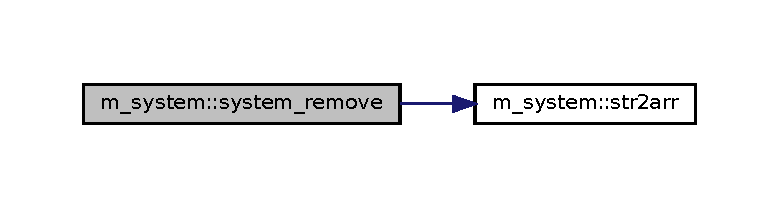
\includegraphics[width=350pt]{namespacem__system_a730ae64294e3cd73bde8f0c63cdf9972_cgraph}
\end{center}
\end{figure}
\mbox{\Hypertarget{namespacem__system_adfbaf3d17790da9ba0c520683d5b8003}\label{namespacem__system_adfbaf3d17790da9ba0c520683d5b8003}} 
\index{m\+\_\+system@{m\+\_\+system}!system\+\_\+rename@{system\+\_\+rename}}
\index{system\+\_\+rename@{system\+\_\+rename}!m\+\_\+system@{m\+\_\+system}}
\subsubsection{\texorpdfstring{system\+\_\+rename()}{system\_rename()}}
{\footnotesize\ttfamily integer function, public m\+\_\+system\+::system\+\_\+rename (\begin{DoxyParamCaption}\item[{character($\ast$), intent(in)}]{input,  }\item[{character($\ast$), intent(in)}]{output }\end{DoxyParamCaption})}



\subsubsection*{N\+A\+ME}

system\+\_\+rename(3f) -\/ \mbox{[}M\+\_\+system\mbox{]} call rename(3c) to rename a system file (L\+I\+C\+E\+N\+SE\+:PD) \subsubsection*{S\+Y\+N\+O\+P\+S\+IS}

function system\+\_\+rename(input,output) result(ierr)

character($\ast$),intent(in) \+:\+: input,output integer \+:\+: ierr \subsubsection*{D\+E\+S\+C\+R\+I\+P\+T\+I\+ON}

Rename a file by calling rename(3c). It is not recommended that the rename occur while either filename is being used on a file currently O\+P\+E\+N(3f) by the program.

Both the old and new names must be on the same device. \subsubsection*{O\+P\+T\+I\+O\+NS}

I\+N\+P\+UT system filename of an existing file to rename O\+U\+T\+P\+UT system filename to be created or overwritten by I\+N\+P\+UT file. Must be on the same device as the I\+N\+P\+UT file. \subsubsection*{R\+E\+T\+U\+R\+NS}

I\+E\+RR zero (0) if no error occurs. If not zero a call to system\+\_\+errno(3f) or system\+\_\+perror(3f) is supported to diagnose error \subsubsection*{E\+X\+A\+M\+P\+LE}

\begin{DoxyVerb}Sample program:

  program demo_system_rename
  use M_system, only : system_rename
  use M_system, only : system_remove
  use M_system, only : system_perror
  implicit none
  character(len=256) :: string
  integer            :: ios, ierr

  ! try to remove junk files just in case
  ierr=system_remove('_scratch_file_')
  write(*,'(a,i0)') 'should not be zero ',ierr
  call system_perror('*demo_system_rename*')
  ierr=system_remove('_renamed_scratch_file_')
  write(*,'(a,i0)') 'should not be zero ',ierr
  call system_perror('*demo_system_rename*')

  ! create scratch file to rename
  open(unit=10,file='_scratch_file_',status='new')
  write(10,'(a)') 'Test by renaming "_scratch_file_" to "_renamed_scratch_file_"'
  write(10,'(a)') 'IF YOU SEE THIS ON OUTPUT THE RENAME WORKED'
  close(10)
  ! rename scratch file
  ierr=system_rename('_scratch_file_','_renamed_scratch_file_')
  if(ierr.ne.0)then
     write(*,*)'ERROR RENAMING FILE ',ierr
  endif
  ! read renamed file
  open(unit=11,file='_renamed_scratch_file_',status='old')
  INFINITE: do
     read(11,'(a)',iostat=ios)string
     if(ios.ne.0)exit INFINITE
     write(*,'(a)')trim(string)
  enddo INFINITE
  close(unit=11)

  ! clean up
  ierr=system_remove('_scratch_file_')
  write(*,'(a,i0)') 'should not be zero ',ierr
  ierr=system_remove('_renamed_scratch_file_')
  write(*,'(a,i0)') 'should be zero ',ierr

  end program demo_system_rename
\end{DoxyVerb}


Expected output\+:

$>$ should not be zero -\/1 $>$ {\itshape demo\+\_\+system\+\_\+rename}\+: No such file or directory $>$ should not be zero -\/1 $>$ {\itshape demo\+\_\+system\+\_\+rename}\+: No such file or directory $>$ Test by renaming \char`\"{}\+\_\+scratch\+\_\+file\+\_\+\char`\"{} to \char`\"{}\+\_\+renamed\+\_\+scratch\+\_\+file\+\_\+\char`\"{} $>$ IF Y\+OU S\+EE T\+H\+IS ON O\+U\+T\+P\+UT T\+HE R\+E\+N\+A\+ME W\+O\+R\+K\+ED $>$ should not be zero -\/1 $>$ should be zero 0

\subsubsection*{A\+U\+T\+H\+OR}

John S. Urban \subsubsection*{L\+I\+C\+E\+N\+SE}

Public Domain 

References str2arr().

Here is the call graph for this function\+:
\nopagebreak
\begin{figure}[H]
\begin{center}
\leavevmode
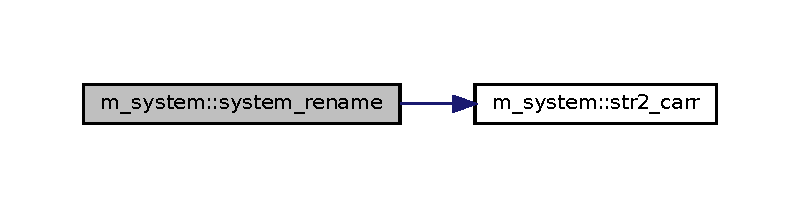
\includegraphics[width=350pt]{namespacem__system_adfbaf3d17790da9ba0c520683d5b8003_cgraph}
\end{center}
\end{figure}
\mbox{\Hypertarget{namespacem__system_a3ffe757195ade8052e8acabd196ee3ca}\label{namespacem__system_a3ffe757195ade8052e8acabd196ee3ca}} 
\index{m\+\_\+system@{m\+\_\+system}!system\+\_\+rewinddir@{system\+\_\+rewinddir}}
\index{system\+\_\+rewinddir@{system\+\_\+rewinddir}!m\+\_\+system@{m\+\_\+system}}
\subsubsection{\texorpdfstring{system\+\_\+rewinddir()}{system\_rewinddir()}}
{\footnotesize\ttfamily subroutine, public m\+\_\+system\+::system\+\_\+rewinddir (\begin{DoxyParamCaption}\item[{type(c\+\_\+ptr), value}]{dir }\end{DoxyParamCaption})}



\subsubsection*{N\+A\+ME}

system\+\_\+rewinddir(3f) -\/ \mbox{[}M\+\_\+system\mbox{]} call rewinddir(3c) to rewind directory stream (L\+I\+C\+E\+N\+SE\+:PD) \subsubsection*{S\+Y\+N\+O\+P\+S\+IS}

subroutine system\+\_\+rewinddir(dir)

type(c\+\_\+ptr),value \+:\+: dir

\subsubsection*{D\+E\+S\+C\+R\+I\+P\+T\+I\+ON}

Return to pointer to the beginning of the list for a currently open directory list.

\subsubsection*{O\+P\+T\+I\+O\+NS}

D\+IR A C\+\_\+pointer assumed to have been allocated by a call to S\+Y\+S\+T\+E\+M\+\_\+\+O\+P\+E\+N\+D\+I\+R(3f).

\subsubsection*{E\+X\+A\+M\+P\+LE}

Sample program\+:

program demo\+\_\+system\+\_\+rewinddir use M\+\_\+system, only \+: system\+\_\+opendir,system\+\_\+readdir use M\+\_\+system, only \+: system\+\_\+rewinddir,system\+\_\+closedir use iso\+\_\+c\+\_\+binding implicit none

type(c\+\_\+ptr) \+:\+: dir character(len=\+:),allocatable \+:\+: filename integer \+:\+: i, ierr !$>$$>$$>$ open directory stream to read from call system\+\_\+opendir(\textquotesingle{}.\textquotesingle{},dir,ierr) !$>$$>$$>$ read directory stream twice do i=1,2 write($\ast$,\textquotesingle{}(a,i0)\textquotesingle{})\textquotesingle{}P\+A\+SS \textquotesingle{},i do call system\+\_\+readdir(dir,filename,ierr) if(filename.\+eq.\textquotesingle{} \textquotesingle{})exit write($\ast$,$\ast$)filename enddo !$>$$>$$>$ rewind directory stream call system\+\_\+rewinddir(dir) enddo !$>$$>$$>$ close directory stream call system\+\_\+closedir(dir,ierr)

end program demo\+\_\+system\+\_\+rewinddir \subsubsection*{A\+U\+T\+H\+OR}

John S. Urban \subsubsection*{L\+I\+C\+E\+N\+SE}

Public Domain \mbox{\Hypertarget{namespacem__system_a21fd3e1ccd50cef6adc539ef3d7a9836}\label{namespacem__system_a21fd3e1ccd50cef6adc539ef3d7a9836}} 
\index{m\+\_\+system@{m\+\_\+system}!system\+\_\+rmdir@{system\+\_\+rmdir}}
\index{system\+\_\+rmdir@{system\+\_\+rmdir}!m\+\_\+system@{m\+\_\+system}}
\subsubsection{\texorpdfstring{system\+\_\+rmdir()}{system\_rmdir()}}
{\footnotesize\ttfamily integer(c\+\_\+int) function, public m\+\_\+system\+::system\+\_\+rmdir (\begin{DoxyParamCaption}\item[{character($\ast$), intent(in)}]{dirname }\end{DoxyParamCaption})}



\subsubsection*{N\+A\+ME}

system\+\_\+rmdir(3f) -\/ \mbox{[}M\+\_\+system\mbox{]} call rmdir(3c) to remove empty directories (L\+I\+C\+E\+N\+SE\+:PD) 

\subsubsection*{S\+Y\+N\+O\+P\+S\+IS}

\begin{DoxyVerb}function system_rmdir(dirname) result(err)

 character(*),intent(in) :: dirname
 integer(c_int) :: err
\end{DoxyVerb}


\subsubsection*{D\+E\+S\+C\+R\+I\+P\+T\+I\+ON}

D\+I\+R\+E\+C\+T\+O\+RY The name of a directory to remove if it is empty err zero (0) if no error occurred

\subsubsection*{E\+X\+A\+M\+P\+LE}

Sample program\+:

program demo\+\_\+system\+\_\+rmdir use M\+\_\+system, only \+: system\+\_\+perror use M\+\_\+system, only \+: system\+\_\+rmdir, system\+\_\+mkdir use M\+\_\+system, only \+: R\+W\+X\+\_\+U implicit none integer \+:\+: ierr write($\ast$,$\ast$)\textquotesingle{}B\+E\+F\+O\+RE T\+RY TO C\+R\+E\+A\+TE \+\_\+scratch/\textquotesingle{} call execute\+\_\+command\+\_\+line(\textquotesingle{}ls -\/ld \+\_\+scratch\textquotesingle{})

write($\ast$,$\ast$)\textquotesingle{}T\+RY TO C\+R\+E\+A\+TE \+\_\+scratch/\textquotesingle{} ierr=system\+\_\+mkdir(\textquotesingle{}\+\_\+scratch\textquotesingle{},R\+W\+X\+\_\+U) write($\ast$,$\ast$)\textquotesingle{}I\+E\+RR=\textquotesingle{},ierr call execute\+\_\+command\+\_\+line(\textquotesingle{}ls -\/ld \+\_\+scratch\textquotesingle{})

write($\ast$,$\ast$)\textquotesingle{}T\+RY TO R\+E\+M\+O\+VE \+\_\+scratch/\textquotesingle{} ierr=system\+\_\+rmdir(\textquotesingle{}\+\_\+scratch\textquotesingle{}) write($\ast$,$\ast$)\textquotesingle{}I\+E\+RR=\textquotesingle{},ierr call execute\+\_\+command\+\_\+line(\textquotesingle{}ls -\/ld \+\_\+scratch\textquotesingle{})

write($\ast$,$\ast$)\textquotesingle{}T\+RY TO R\+E\+M\+O\+VE \+\_\+scratch when it should be gone/\textquotesingle{} ierr=system\+\_\+rmdir(\textquotesingle{}\+\_\+scratch\textquotesingle{}) call system\+\_\+perror(\textquotesingle{}{\itshape test of system\+\_\+rmdir}\textquotesingle{}) write($\ast$,$\ast$)\textquotesingle{}I\+E\+RR=\textquotesingle{},ierr call execute\+\_\+command\+\_\+line(\textquotesingle{}ls -\/ld \+\_\+scratch\textquotesingle{})

end program demo\+\_\+system\+\_\+rmdir

Expected output\+:

\subsubsection*{A\+U\+T\+H\+OR}

John S. Urban \subsubsection*{L\+I\+C\+E\+N\+SE}

Public Domain 

References str2arr().

Here is the call graph for this function\+:
\nopagebreak
\begin{figure}[H]
\begin{center}
\leavevmode
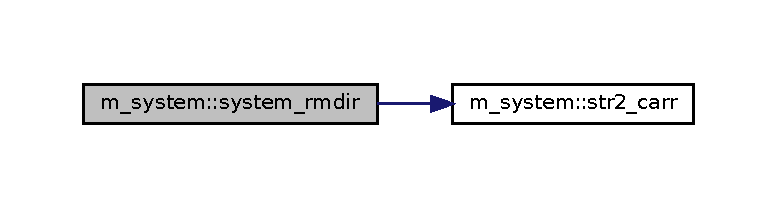
\includegraphics[width=350pt]{namespacem__system_a21fd3e1ccd50cef6adc539ef3d7a9836_cgraph}
\end{center}
\end{figure}
\mbox{\Hypertarget{namespacem__system_a04fd02e6f5ce2f8ecdfb577e1490feba}\label{namespacem__system_a04fd02e6f5ce2f8ecdfb577e1490feba}} 
\index{m\+\_\+system@{m\+\_\+system}!system\+\_\+setumask@{system\+\_\+setumask}}
\index{system\+\_\+setumask@{system\+\_\+setumask}!m\+\_\+system@{m\+\_\+system}}
\subsubsection{\texorpdfstring{system\+\_\+setumask()}{system\_setumask()}}
{\footnotesize\ttfamily integer function, public m\+\_\+system\+::system\+\_\+setumask (\begin{DoxyParamCaption}\item[{integer, intent(in)}]{umask\+\_\+value }\end{DoxyParamCaption})}



\subsubsection*{N\+A\+ME}

system\+\_\+setumask(3f) -\/ \mbox{[}M\+\_\+system\mbox{]} set the file mode creation umask (L\+I\+C\+E\+N\+SE\+:PD) \subsubsection*{S\+Y\+N\+O\+P\+S\+IS}

integer function system\+\_\+setumask(new\+\_\+umask) result (old\+\_\+umask)

integer,intent(in) \+:\+: new\+\_\+umask integer(kind=c\+\_\+int) \+:\+: umask\+\_\+c

\subsubsection*{D\+E\+S\+C\+R\+I\+P\+T\+I\+ON}

The system\+\_\+umask(3f) function sets the file mode creation mask of the process to cmask and return the previous value of the mask. Only the file permission bits of cmask (see $<$sys/stat.\+h$>$) are used; the meaning of the other bits is implementation-\/defined.

The file mode creation mask of the process is used to turn off permission bits in the mode argument supplied during calls to the following functions\+:


\begin{DoxyItemize}
\item open(), openat(), creat(), mkdir(), mkdirat(), mkfifo(), and mkfifoat()
\item mknod(), mknodat()
\item mq\+\_\+open()
\item sem\+\_\+open()
\end{DoxyItemize}

Bit positions that are set in cmask are cleared in the mode of the created file.

\subsubsection*{R\+E\+T\+U\+RN V\+A\+L\+UE}

The file permission bits in the value returned by umask() shall be the previous value of the file mode creation mask. The state of any other bits in that value is unspecified, except that a subsequent call to umask() with the returned value as cmask shall leave the state of the mask the same as its state before the first call, including any unspecified use of those bits.

\subsubsection*{E\+R\+R\+O\+RS}

No errors are defined.

\subsubsection*{E\+X\+A\+M\+P\+LE}

Sample program

program demo\+\_\+setumask use M\+\_\+system, only \+: system\+\_\+getumask, system\+\_\+setumask integer \+:\+: newmask integer \+:\+: i integer \+:\+: old\+\_\+umask write($\ast$,101)(\mbox{\hyperlink{namespacem__system_aa9ca951be39d2ea738d627cf42c00ddd}{system\+\_\+getumask()}},i=1,4) 101 format(1x,i0,1x,\char`\"{}\+O\textquotesingle{}\char`\"{},o4.\+4,\char`\"{}\textquotesingle{}\char`\"{},1x,\textquotesingle{}Z\char`\"{}\textquotesingle{},z0,\char`\"{}\textquotesingle{}\char`\"{},1x,\char`\"{}B\textquotesingle{}\char`\"{},b12.\+12,\char`\"{}\textquotesingle{}") newmask=63 old\+\_\+umask=system\+\_\+setumask(newmask) write($\ast$,$\ast$)\textquotesingle{}N\+EW\textquotesingle{} write($\ast$,101)(\mbox{\hyperlink{namespacem__system_aa9ca951be39d2ea738d627cf42c00ddd}{system\+\_\+getumask()}},i=1,4) end program demo\+\_\+setumask

Expected output

18 O\textquotesingle{}022\textquotesingle{} Z\char`\"{}12\textquotesingle{} B\textquotesingle{}000010010\char`\"{} N\+EW 63 O\textquotesingle{}077\textquotesingle{} Z\char`\"{}3\+F\textquotesingle{} B\textquotesingle{}000111111\char`\"{} \mbox{\Hypertarget{namespacem__system_a5bb1ebcebe181e07fd24e908cacc9887}\label{namespacem__system_a5bb1ebcebe181e07fd24e908cacc9887}} 
\index{m\+\_\+system@{m\+\_\+system}!system\+\_\+stat@{system\+\_\+stat}}
\index{system\+\_\+stat@{system\+\_\+stat}!m\+\_\+system@{m\+\_\+system}}
\subsubsection{\texorpdfstring{system\+\_\+stat()}{system\_stat()}}
{\footnotesize\ttfamily subroutine, public m\+\_\+system\+::system\+\_\+stat (\begin{DoxyParamCaption}\item[{character(len=$\ast$), intent(in)}]{pathname,  }\item[{integer(kind=int64), dimension(13), intent(out)}]{values,  }\item[{integer, intent(out), optional}]{ierr }\end{DoxyParamCaption})}



\subsubsection*{N\+A\+ME}

S\+Y\+S\+T\+E\+M\+\_\+\+S\+T\+AT -\/ \mbox{[}M\+\_\+system\mbox{]} Get file status information (L\+I\+C\+E\+N\+SE\+:PD) 

\subsubsection*{S\+Y\+N\+T\+AX}

C\+A\+LL S\+Y\+S\+T\+E\+M\+\_\+\+S\+T\+A\+T(\+N\+A\+M\+E, V\+A\+L\+U\+E\+S \mbox{[}, S\+T\+A\+T\+U\+S\mbox{]},\mbox{[}\+D\+E\+B\+U\+G\mbox{]})

character(len=$\ast$),intent(in) \+:\+: N\+A\+ME integer(kind=int64),intent(out) \+:\+: values(13) integer,optional,intent(out) \+:\+: status integer,intent(in) \+:\+: debug

\subsubsection*{D\+E\+S\+C\+R\+I\+P\+T\+I\+ON}

\begin{DoxyVerb}This function returns information about a file. No permissions are
required on the file itself, but execute (search) permission is required
on all of the directories in path that lead to the file. The elements
that are obtained and stored in the array VALUES:

   VALUES(1) Device ID
   VALUES(2) Inode number
   VALUES(3) File mode
   VALUES(4) Number of links
   VALUES(5) Owner's uid
   VALUES(6) Owner's gid
   VALUES(7) ID of device containing directory entry for file (0 if not available)
   VALUES(8) File size (bytes)
   VALUES(9) Last access time as a Unix Epoch time rounded to seconds
   VALUES(10) Last modification time as a Unix Epoch time rounded to seconds
   VALUES(11) Last file status change time as a Unix Epoch time rounded to seconds
   VALUES(12) Preferred I/O block size (-1 if not available)
   VALUES(13) Number of blocks allocated (-1 if not available)

Not all these elements are relevant on all systems. If an element is
not relevant, it is returned as 0.
\end{DoxyVerb}


\subsubsection*{O\+P\+T\+I\+O\+NS}

\begin{DoxyVerb}NAME    The type shall be CHARACTER, of the default kind and a valid
        path within the file system.
VALUES  The type shall be INTEGER(8), DIMENSION(13).
STATUS  (Optional) status flag of type INTEGER(4). Returns 0 on success
        and a system specific error code otherwise.
DEBUG   (Optional) print values being returned from C routine being
        called if value of 0 is used
\end{DoxyVerb}


\subsubsection*{E\+X\+A\+M\+P\+LE}

program demo\+\_\+system\+\_\+stat

use M\+\_\+system, only \+: system\+\_\+stat, system\+\_\+getpwuid, system\+\_\+getgrgid use M\+\_\+time, only \+: fmtdate, u2d use, intrinsic \+:\+: iso\+\_\+fortran\+\_\+env, only \+: int32, int64 implicit none

integer(kind=int64) \+:\+: buff(13) integer(kind=int32) \+:\+: status character(len=$\ast$),parameter \+:\+: fmt\+\_\+date=\textquotesingle{}year-\/month-\/day hour\+:minute\+:second\textquotesingle{}

integer(kind=int64) \+:\+: \& Device\+\_\+\+ID, Inode\+\_\+number, File\+\_\+mode, Number\+\_\+of\+\_\+links, Owner\+\_\+uid, \& Owner\+\_\+gid, Directory\+\_\+device, File\+\_\+size, Last\+\_\+access, Last\+\_\+modification, \& Last\+\_\+status\+\_\+change, Preferred\+\_\+block\+\_\+size, Number\+\_\+of\+\_\+blocks\+\_\+allocated equivalence \& ( buff(1) , Device\+\_\+\+ID ) , \& ( buff(2) , Inode\+\_\+number ) , \& ( buff(3) , File\+\_\+mode ) , \& ( buff(4) , Number\+\_\+of\+\_\+links ) , \& ( buff(5) , Owner\+\_\+uid ) , \& ( buff(6) , Owner\+\_\+gid ) , \& ( buff(7) , Directory\+\_\+device ) , \& ( buff(8) , File\+\_\+size ) , \& ( buff(9) , Last\+\_\+access ) , \& ( buff(10) , Last\+\_\+modification ) , \& ( buff(11) , Last\+\_\+status\+\_\+change ) , \& ( buff(12) , Preferred\+\_\+block\+\_\+size ) , \& ( buff(13) , Number\+\_\+of\+\_\+blocks\+\_\+allocated )

C\+A\+LL S\+Y\+S\+T\+E\+M\+\_\+\+S\+T\+AT(\char`\"{}/etc/hosts\char`\"{}, buff, status)

if (status == 0) then write ($\ast$, F\+MT=\char`\"{}(\textquotesingle{}\+Device I\+D(hex/decimal)\+:\textquotesingle{},      T30, Z0,\textquotesingle{}h/\textquotesingle{},\+I0,\textquotesingle{}d\textquotesingle{})\char`\"{}) buff(1),buff(1) write ($\ast$, F\+MT=\char`\"{}(\textquotesingle{}\+Inode number\+:\textquotesingle{},                T30, I0)\char`\"{}) buff(2) write ($\ast$, F\+MT=\char`\"{}(\textquotesingle{}\+File mode (octal)\+:\textquotesingle{},           T30, O19)\char`\"{}) buff(3) write ($\ast$, F\+MT=\char`\"{}(\textquotesingle{}\+Number of links\+:\textquotesingle{},             T30, I0)\char`\"{}) buff(4) write ($\ast$, F\+MT=\char`\"{}(\textquotesingle{}\+Owner\textquotesingle{}\textquotesingle{}s uid/username\+:\textquotesingle{},       T30, I0,1x, A)\char`\"{}) buff(5), system\+\_\+getpwuid(buff(5)) write ($\ast$, F\+MT=\char`\"{}(\textquotesingle{}\+Owner\textquotesingle{}\textquotesingle{}s gid/group\+:\textquotesingle{},          T30, I0,1x, A)\char`\"{}) buff(6), system\+\_\+getgrgid(buff(6)) write ($\ast$, F\+MT=\char`\"{}(\textquotesingle{}\+Device where located\+:\textquotesingle{},        T30, I0)\char`\"{}) buff(7) write ($\ast$, F\+MT=\char`\"{}(\textquotesingle{}\+File size(bytes)\+:\textquotesingle{},            T30, I0)\char`\"{}) buff(8) write ($\ast$, F\+MT=\char`\"{}(\textquotesingle{}\+Last access time\+:\textquotesingle{},            T30, I0,1x, A)\char`\"{}) buff(9), fmtdate(u2d(int(buff(9))),fmt\+\_\+date) write ($\ast$, F\+MT=\char`\"{}(\textquotesingle{}\+Last modification time\+:\textquotesingle{},      T30, I0,1x, A)\char`\"{}) buff(10),fmtdate(u2d(int(buff(10))),fmt\+\_\+date) write ($\ast$, F\+MT=\char`\"{}(\textquotesingle{}\+Last status change time\+:\textquotesingle{},     T30, I0,1x, A)\char`\"{}) buff(11),fmtdate(u2d(int(buff(11))),fmt\+\_\+date) write ($\ast$, F\+MT=\char`\"{}(\textquotesingle{}\+Preferred block size(bytes)\+:\textquotesingle{}, T30, I0)\char`\"{}) buff(12) write ($\ast$, F\+MT=\char`\"{}(\textquotesingle{}\+No. of blocks allocated\+:\textquotesingle{},     T30, I0)\char`\"{}) buff(13) endif

end program demo\+\_\+system\+\_\+stat

Results\+:

Device ID(hex/decimal)\+: 3\+E6\+B\+E045h/1047257157d Inode number\+: 1407374886070599 File mode (octal)\+: 100750 Number of links\+: 1 Owner\textquotesingle{}s uid/username\+: 18 S\+Y\+S\+T\+EM Owner\textquotesingle{}s gid/group\+: 18 S\+Y\+S\+T\+EM Device where located\+: 0 File size(bytes)\+: 824 Last access time\+: 1557983191 2019-\/05-\/16 01\+:06\+:31 Last modification time\+: 1557983191 2019-\/05-\/16 01\+:06\+:31 Last status change time\+: 1557983532 2019-\/05-\/16 01\+:12\+:12 Preferred block size(bytes)\+: 65536 No. of blocks allocated\+: 4

\subsubsection*{A\+U\+T\+H\+OR}

John S. Urban \subsubsection*{L\+I\+C\+E\+N\+SE}

Public Domain 

References str2arr().

Here is the call graph for this function\+:
\nopagebreak
\begin{figure}[H]
\begin{center}
\leavevmode
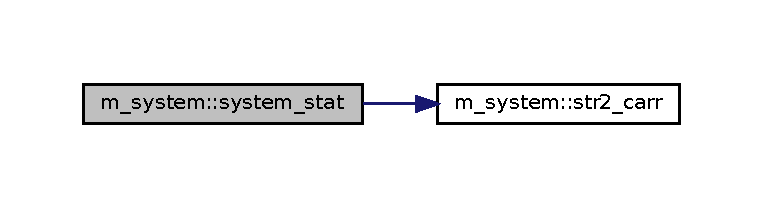
\includegraphics[width=350pt]{namespacem__system_a5bb1ebcebe181e07fd24e908cacc9887_cgraph}
\end{center}
\end{figure}
\mbox{\Hypertarget{namespacem__system_a04e5d49509c44bcb2ccabfd80ec8cdfb}\label{namespacem__system_a04e5d49509c44bcb2ccabfd80ec8cdfb}} 
\index{m\+\_\+system@{m\+\_\+system}!system\+\_\+uname@{system\+\_\+uname}}
\index{system\+\_\+uname@{system\+\_\+uname}!m\+\_\+system@{m\+\_\+system}}
\subsubsection{\texorpdfstring{system\+\_\+uname()}{system\_uname()}}
{\footnotesize\ttfamily subroutine, public m\+\_\+system\+::system\+\_\+uname (\begin{DoxyParamCaption}\item[{character(kind=c\+\_\+char), intent(in)}]{W\+H\+I\+CH,  }\item[{character(len=$\ast$), intent(out)}]{N\+A\+M\+E\+O\+UT }\end{DoxyParamCaption})}



\subsubsection*{N\+A\+ME}

system\+\_\+uname(3f) -\/ \mbox{[}M\+\_\+system\mbox{]} call a C wrapper that calls uname(3c) to get current system information from Fortran (L\+I\+C\+E\+N\+SE\+:PD) \subsubsection*{S\+Y\+N\+O\+P\+S\+IS}

subroutine system\+\_\+uname(\+W\+H\+I\+C\+H,\+N\+A\+M\+E\+O\+U\+T)

character(K\+I\+ND=C\+\_\+\+C\+H\+AR),intent(in) \+:\+: W\+H\+I\+CH character(len=$\ast$),intent(out) \+:\+: N\+A\+M\+E\+O\+UT \subsubsection*{D\+E\+S\+C\+R\+I\+P\+T\+I\+ON}

Given a letter, return a corresponding description of the current operating system. The N\+A\+M\+E\+O\+UT variable is assumed sufficiently large enough to hold the value.

s return the kernel name r return the kernel release v return the kernel version n return the network node hostname m return the machine hardware name T test mode -- print all information, in the following order -\/ srvnm

\subsubsection*{E\+X\+A\+M\+P\+LE}

Call uname(3c) from Fortran

program demo\+\_\+system\+\_\+uname use M\+\_\+system, only \+: system\+\_\+uname implicit none integer,parameter \+:\+: is=100 integer \+:\+: i character(len=$\ast$),parameter \+:\+: letters=\textquotesingle{}srvnmxT\textquotesingle{} character(len=is) \+:\+: string=\textquotesingle{} \textquotesingle{}

do i=1,len(letters) write($\ast$,\textquotesingle{}(80(\char`\"{}=\char`\"{}))\textquotesingle{}) call system\+\_\+uname(letters(i\+:i),string) write($\ast$,$\ast$)\textquotesingle{}=====$>$ T\+E\+S\+T\+I\+NG system\+\_\+uname(\textquotesingle{}//letters(i\+:i)//\textquotesingle{})---$>$\textquotesingle{}//trim(string) enddo

end program demo\+\_\+system\+\_\+uname \subsubsection*{A\+U\+T\+H\+OR}

John S. Urban \subsubsection*{L\+I\+C\+E\+N\+SE}

Public Domain \mbox{\Hypertarget{namespacem__system_a14ce0b9177815bc357dbdf3778687bb7}\label{namespacem__system_a14ce0b9177815bc357dbdf3778687bb7}} 
\index{m\+\_\+system@{m\+\_\+system}!system\+\_\+unlink@{system\+\_\+unlink}}
\index{system\+\_\+unlink@{system\+\_\+unlink}!m\+\_\+system@{m\+\_\+system}}
\subsubsection{\texorpdfstring{system\+\_\+unlink()}{system\_unlink()}}
{\footnotesize\ttfamily integer function, public m\+\_\+system\+::system\+\_\+unlink (\begin{DoxyParamCaption}\item[{character(len=$\ast$), intent(in)}]{fname }\end{DoxyParamCaption})}



\subsubsection*{N\+A\+ME}

system\+\_\+unlink(3f) -\/ \mbox{[}M\+\_\+system\mbox{]} remove a directory entry relative to directory file descriptor (L\+I\+C\+E\+N\+SE\+:PD) 

\subsubsection*{S\+Y\+N\+O\+P\+S\+IS}

\begin{DoxyVerb}integer function unlink(path);

 character(len=*) :: path
\end{DoxyVerb}


\subsubsection*{D\+E\+S\+C\+R\+I\+P\+T\+I\+ON}

The unlink() function shall remove a link to a file. If path names a symbolic link, unlink() shall remove the symbolic link named by path and shall not affect any file or directory named by the contents of the symbolic link. Otherwise, unlink() shall remove the link named by the pathname pointed to by path and shall decrement the link count of the file referenced by the link.

When the file\textquotesingle{}s link count becomes 0 and no process has the file open, the space occupied by the file shall be freed and the file shall no longer be accessible. If one or more processes have the file open when the last link is removed, the link shall be removed before unlink() returns, but the removal of the file contents shall be postponed until all references to the file are closed.

The path argument shall not name a directory unless the process has appropriate privileges and the implementation supports using unlink() on directories.

Upon successful completion, unlink() shall mark for update the last data modification and last file status change timestamps of the parent directory. Also, if the file\textquotesingle{}s link count is not 0, the last file status change timestamp of the file shall be marked for update.

Values for flag are constructed by a bitwise-\/inclusive OR of flags from the following list, defined in $<$fcntl.\+h$>$\+:

A\+T\+\_\+\+R\+E\+M\+O\+V\+E\+D\+IR

Remove the directory entry specified by fd and path as a directory, not a normal file.

\subsubsection*{R\+E\+T\+U\+RN V\+A\+L\+UE}

\begin{DoxyVerb}Upon successful completion, these functions shall return 0. Otherwise,
these functions shall return -1 and set errno to indicate the error. If
-1 is returned, the named file shall not be changed.
\end{DoxyVerb}


\subsubsection*{E\+X\+A\+M\+P\+L\+ES}

Removing a link to a file

program demo\+\_\+system\+\_\+unlink use M\+\_\+system, only \+: system\+\_\+unlink, system\+\_\+perror integer \+:\+: ierr ierr = system\+\_\+unlink(\textquotesingle{}myfile1\textquotesingle{}) if(ierr.\+ne.\+0)then call system\+\_\+perror(\textquotesingle{}{\itshape demo\+\_\+system\+\_\+unlink}\textquotesingle{}) endif end program demo\+\_\+system\+\_\+unlink 

References str2arr().

Here is the call graph for this function\+:
\nopagebreak
\begin{figure}[H]
\begin{center}
\leavevmode
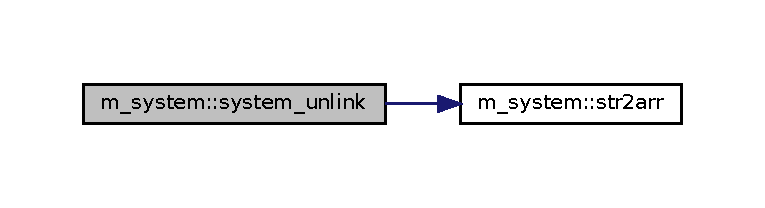
\includegraphics[width=350pt]{namespacem__system_a14ce0b9177815bc357dbdf3778687bb7_cgraph}
\end{center}
\end{figure}
\mbox{\Hypertarget{namespacem__system_a61b67b46b35490ec308773b65c3376a3}\label{namespacem__system_a61b67b46b35490ec308773b65c3376a3}} 
\index{m\+\_\+system@{m\+\_\+system}!system\+\_\+unsetenv@{system\+\_\+unsetenv}}
\index{system\+\_\+unsetenv@{system\+\_\+unsetenv}!m\+\_\+system@{m\+\_\+system}}
\subsubsection{\texorpdfstring{system\+\_\+unsetenv()}{system\_unsetenv()}}
{\footnotesize\ttfamily subroutine, public m\+\_\+system\+::system\+\_\+unsetenv (\begin{DoxyParamCaption}\item[{character(len=$\ast$), intent(in)}]{name,  }\item[{integer, intent(out), optional}]{ierr }\end{DoxyParamCaption})}



\subsubsection*{N\+A\+ME}

system\+\_\+unsetenv(3f) -\/ \mbox{[}M\+\_\+system\+:E\+N\+V\+I\+R\+O\+N\+M\+E\+NT\mbox{]} delete an environment variable by calling unsetenv(3c) (L\+I\+C\+E\+N\+SE\+:PD) \subsubsection*{S\+Y\+N\+O\+P\+S\+IS}

subroutine system\+\_\+unsetenv(name,ierr)

character(len=$\ast$),intent(in) \+:\+: name integer,intent(out),optional \+:\+: ierr

\subsubsection*{D\+E\+S\+C\+R\+I\+P\+T\+I\+ON}

\begin{DoxyVerb}The system_unsetenv(3f) function deletes the variable name from the
environment.
\end{DoxyVerb}


\subsubsection*{O\+P\+T\+I\+O\+NS}

name name of variable to delete. If name does not exist in the environment, then the function succeeds, and the environment is unchanged.

ierr The system\+\_\+unsetenv(3f) function returns zero on success, or -\/1 on error. name is N\+U\+LL, points to a string of length 0, or contains an \textquotesingle{}=\textquotesingle{} character. Insufficient memory to add a new variable to the environment.

\subsubsection*{E\+X\+A\+M\+P\+LE}

Sample program\+:

program demo\+\_\+system\+\_\+unsetenv use M\+\_\+system, only \+: system\+\_\+unsetenv, system\+\_\+putenv implicit none call system\+\_\+putenv(\textquotesingle{}G\+RU=this is the value\textquotesingle{}) write($\ast$,\textquotesingle{}(a)\textquotesingle{})\textquotesingle{}The variable G\+RU should be set\textquotesingle{} call execute\+\_\+command\+\_\+line(\textquotesingle{}env$\vert$grep G\+RU\textquotesingle{}) call system\+\_\+unsetenv(\textquotesingle{}G\+RU\textquotesingle{}) write($\ast$,\textquotesingle{}(a)\textquotesingle{})\textquotesingle{}The variable G\+RU should not be set\textquotesingle{} call execute\+\_\+command\+\_\+line(\textquotesingle{}env$\vert$grep G\+RU\textquotesingle{}) end program demo\+\_\+system\+\_\+unsetenv

\subsubsection*{A\+U\+T\+H\+OR}

John S. Urban \subsubsection*{L\+I\+C\+E\+N\+SE}

Public Domain 

References str2arr().

Here is the call graph for this function\+:
\nopagebreak
\begin{figure}[H]
\begin{center}
\leavevmode
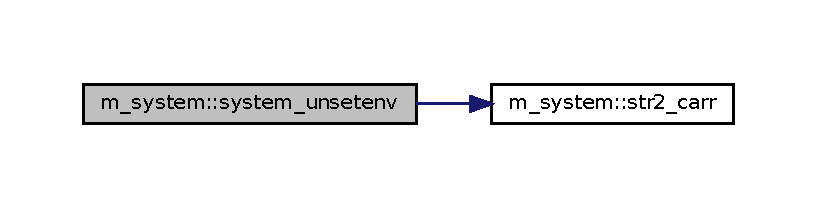
\includegraphics[width=350pt]{namespacem__system_a61b67b46b35490ec308773b65c3376a3_cgraph}
\end{center}
\end{figure}
Here is the caller graph for this function\+:
\nopagebreak
\begin{figure}[H]
\begin{center}
\leavevmode
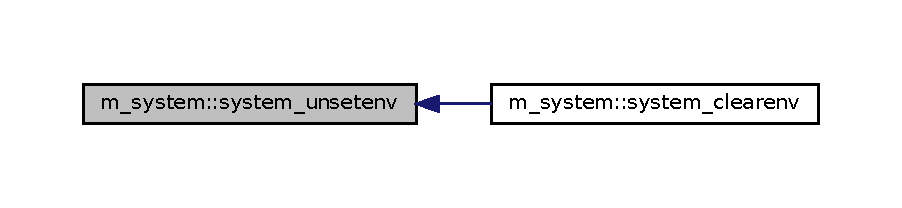
\includegraphics[width=350pt]{namespacem__system_a61b67b46b35490ec308773b65c3376a3_icgraph}
\end{center}
\end{figure}
\mbox{\Hypertarget{namespacem__system_a83a121ba0b525210b5217565569ef350}\label{namespacem__system_a83a121ba0b525210b5217565569ef350}} 
\index{m\+\_\+system@{m\+\_\+system}!system\+\_\+utime@{system\+\_\+utime}}
\index{system\+\_\+utime@{system\+\_\+utime}!m\+\_\+system@{m\+\_\+system}}
\subsubsection{\texorpdfstring{system\+\_\+utime()}{system\_utime()}}
{\footnotesize\ttfamily logical function, public m\+\_\+system\+::system\+\_\+utime (\begin{DoxyParamCaption}\item[{character(len=$\ast$), intent(in)}]{pathname,  }\item[{integer, dimension(2), intent(in)}]{times }\end{DoxyParamCaption})}



\subsubsection*{N\+A\+ME}

system\+\_\+utime(3f) -\/ \mbox{[}M\+\_\+system\mbox{]} set file access and modification times (L\+I\+C\+E\+N\+SE\+:PD) 

\subsubsection*{S\+Y\+N\+O\+P\+S\+IS}

\begin{DoxyVerb}    function utime(pathname,times)

     character(len=*),intent(in) :: pathname
     integer,intent(in)          :: times(2)
     logical                     :: utime
\end{DoxyVerb}


\subsubsection*{D\+E\+S\+C\+R\+I\+P\+T\+I\+ON}

The system\+\_\+utime(3f) function sets the access and modification times of the file named by the path argument by calling utime(3c).

If times() is not present the access and modification times of the file shall be set to the current time.

To use system\+\_\+utime(3f) the effective user ID of the process must match the owner of the file, or the process has to have write permission to the file or have appropriate privileges,

\subsubsection*{O\+P\+T\+I\+O\+NS}

times The values will be interpreted as the access and modification times as Unix Epoch values. That is, they are times measured in seconds since the Unix Epoch.

pathname name of the file whose access and modification times are to be updated.

\subsubsection*{R\+E\+T\+U\+RN V\+A\+L\+UE}

Upon successful completion .T\+R\+UE. is returned. Otherwise, .F\+A\+L\+SE. is returned and errno shall be set to indicate the error, and the file times remain unaffected.

\subsubsection*{E\+R\+R\+O\+RS}

The underlying utime(3c) function fails if\+:

E\+A\+C\+C\+ES Search permission is denied by a component of the path prefix; or the times argument is a null pointer and the effective user ID of the process does not match the owner of the file, the process does not have write permission for the file, and the process does not have appropriate privileges.

E\+L\+O\+OP A loop exists in symbolic links encountered during resolution of the path argument.

E\+N\+A\+M\+E\+T\+O\+O\+L\+O\+NG The length of a component of a pathname is longer than \{N\+A\+M\+E\+\_\+\+M\+AX\}.

E\+N\+O\+E\+NT A component of path does not name an existing file or path is an empty string.

E\+N\+O\+T\+D\+IR A component of the path prefix names an existing file that is neither a directory nor a symbolic link to a directory, or the path argument contains at least one non-\/$<$slash$>$ character and ends with one or more trailing $<$slash$>$ characters and the last pathname component names an existing file that is neither a directory nor a symbolic link to a directory.

E\+P\+E\+RM The times argument is not a null pointer and the effective user ID of the calling process does not match the owner of the file and the calling process does not have appropriate privileges.

E\+R\+O\+FS The file system containing the file is read-\/only.

The utime() function may fail if\+: \begin{DoxyVerb} ELOOP  More than {SYMLOOP_MAX} symbolic links were encountered
        during resolution of the path argument.

 ENAMETOOLONG  The length of a pathname exceeds {PATH_MAX}, or
               pathname resolution of a symbolic link produced
               an intermediate result with a length that exceeds
               {PATH_MAX}.
\end{DoxyVerb}


\subsubsection*{E\+X\+A\+M\+P\+L\+ES}

\begin{DoxyVerb}  Sample program

   program demo_system_utime
   use M_system, only : system_utime, system_perror
   implicit none
   character(len=4096) :: pathname
   integer             :: times(2)
   integer             :: i
      do i=1,command_argument_count()
         call get_command_argument(i, pathname)
         if(.not.system_utime(pathname,times))then
            call system_perror('*demo_system_utime*')
         endif
      enddo
   end program demo_system_utime \end{DoxyVerb}
 

References str2arr().

Here is the call graph for this function\+:
\nopagebreak
\begin{figure}[H]
\begin{center}
\leavevmode
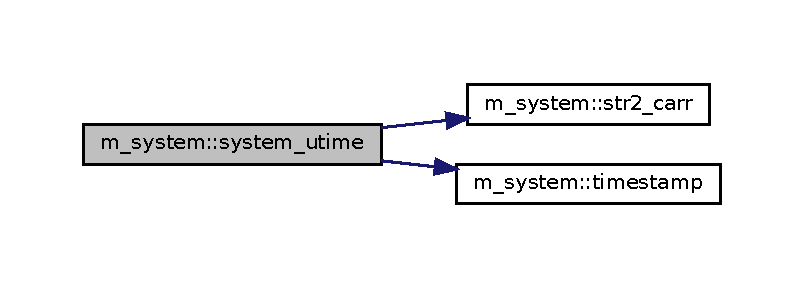
\includegraphics[width=350pt]{namespacem__system_a83a121ba0b525210b5217565569ef350_cgraph}
\end{center}
\end{figure}
\mbox{\Hypertarget{namespacem__system_a403bef1f7fdc42dd75a5b082a15237ff}\label{namespacem__system_a403bef1f7fdc42dd75a5b082a15237ff}} 
\index{m\+\_\+system@{m\+\_\+system}!uniq@{uniq}}
\index{uniq@{uniq}!m\+\_\+system@{m\+\_\+system}}
\subsubsection{\texorpdfstring{uniq()}{uniq()}}
{\footnotesize\ttfamily character(len=\+:) function, allocatable m\+\_\+system\+::uniq (\begin{DoxyParamCaption}\item[{character(len=$\ast$), intent(in)}]{name,  }\item[{integer, intent(in), optional}]{istart,  }\item[{logical, intent(in), optional}]{verbose,  }\item[{logical, intent(in), optional}]{create }\end{DoxyParamCaption})\hspace{0.3cm}{\ttfamily [private]}}

Here is the caller graph for this function\+:
\nopagebreak
\begin{figure}[H]
\begin{center}
\leavevmode
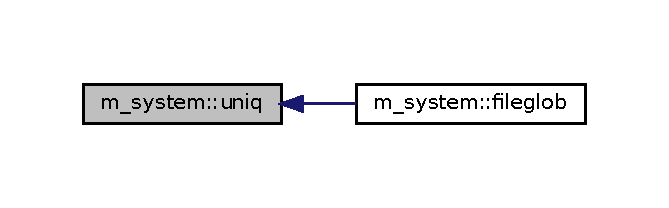
\includegraphics[width=321pt]{namespacem__system_a403bef1f7fdc42dd75a5b082a15237ff_icgraph}
\end{center}
\end{figure}


\subsection{Variable Documentation}
\mbox{\Hypertarget{namespacem__system_a82a13cb7ac2c5f0e6e34fc3cfc010d42}\label{namespacem__system_a82a13cb7ac2c5f0e6e34fc3cfc010d42}} 
\index{m\+\_\+system@{m\+\_\+system}!accessperms@{accessperms}}
\index{accessperms@{accessperms}!m\+\_\+system@{m\+\_\+system}}
\subsubsection{\texorpdfstring{accessperms}{accessperms}}
{\footnotesize\ttfamily integer(kind=\mbox{\hyperlink{namespacem__system_abdb5cc27c945379d844db4830d499050}{mode\+\_\+t}}), public m\+\_\+system\+::accessperms}

\mbox{\Hypertarget{namespacem__system_a7d597052e9d23e2d899e6f81a4509c70}\label{namespacem__system_a7d597052e9d23e2d899e6f81a4509c70}} 
\index{m\+\_\+system@{m\+\_\+system}!bind@{bind}}
\index{bind@{bind}!m\+\_\+system@{m\+\_\+system}}
\subsubsection{\texorpdfstring{bind}{bind}}
{\footnotesize\ttfamily integer(kind=\mbox{\hyperlink{namespacem__system_abdb5cc27c945379d844db4830d499050}{mode\+\_\+t}}), dimension(c,name=\char`\"{}fhost\+\_\+name\+\_\+max\char`\"{}) m\+\_\+system\+::bind\hspace{0.3cm}{\ttfamily [private]}}



\subsubsection*{N\+A\+ME}

system\+\_\+initenv(3f) -\/ \mbox{[}M\+\_\+system\+:E\+N\+V\+I\+R\+O\+N\+M\+E\+NT\mbox{]} initialize environment table pointer and size so table can be read by readenv(3f) (L\+I\+C\+E\+N\+SE\+:PD) \subsubsection*{S\+Y\+N\+O\+P\+S\+IS}

subroutine system\+\_\+initenv() \subsubsection*{D\+E\+S\+C\+R\+I\+P\+T\+I\+ON}

A simple interface allows reading the environment variable table of the process. Call system\+\_\+initenv(3f) to initialize reading the environment table, then call system\+\_\+readenv(3f) until a blank line is returned. If more than one thread reads the environment or the environment is changed while being read the results are undefined.

\subsubsection*{E\+X\+A\+M\+P\+LE}

Sample program\+:

program demo\+\_\+system\+\_\+initenv use M\+\_\+system, only \+: \mbox{\hyperlink{interfacem__system_1_1system__initenv}{system\+\_\+initenv}}, system\+\_\+readenv character(len=\+:),allocatable \+:\+: string call system\+\_\+initenv() do string=\mbox{\hyperlink{namespacem__system_ae0e43010a82a6a25402568ccb326322d}{system\+\_\+readenv()}} if(string.\+eq.\textquotesingle{}\textquotesingle{})then exit else write($\ast$,\textquotesingle{}(a)\textquotesingle{})string endif enddo end program demo\+\_\+system\+\_\+initenv

Sample results\+:

U\+S\+E\+R\+D\+O\+M\+A\+I\+N\+\_\+\+R\+O\+A\+M\+I\+N\+G\+P\+R\+O\+F\+I\+LE=buzz H\+O\+M\+E\+P\+A\+TH= A\+P\+P\+D\+A\+TA=C\+: M\+A\+N\+P\+A\+TH=/home/urbanjs/\+V600/\+L\+I\+B\+R\+A\+R\+Y/lib\+G\+P\+F/download/tmp/man\+:/home/urbanjs/\+V600/doc/man\+:\+:\+: D\+I\+S\+P\+L\+A\+Y\+N\+UM=0 Program\+W6432=C\+: Files H\+O\+S\+T\+N\+A\+ME=buzz X\+K\+E\+Y\+S\+Y\+M\+DB=/usr/share/\+X11/\+X\+Keysym\+DB P\+U\+B\+L\+I\+S\+H\+\_\+\+C\+MD= Online\+Services=Online Services \+: \+: \+: \mbox{\Hypertarget{namespacem__system_a04a5b1ef384bcbb8ad3b0c81ce95001a}\label{namespacem__system_a04a5b1ef384bcbb8ad3b0c81ce95001a}} 
\index{m\+\_\+system@{m\+\_\+system}!deffilemode@{deffilemode}}
\index{deffilemode@{deffilemode}!m\+\_\+system@{m\+\_\+system}}
\subsubsection{\texorpdfstring{deffilemode}{deffilemode}}
{\footnotesize\ttfamily integer(kind=\mbox{\hyperlink{namespacem__system_abdb5cc27c945379d844db4830d499050}{mode\+\_\+t}}), public m\+\_\+system\+::deffilemode}

\mbox{\Hypertarget{namespacem__system_ad34c4f18dd5b7dbe445cca25bbae9a74}\label{namespacem__system_ad34c4f18dd5b7dbe445cca25bbae9a74}} 
\index{m\+\_\+system@{m\+\_\+system}!f\+\_\+ok@{f\+\_\+ok}}
\index{f\+\_\+ok@{f\+\_\+ok}!m\+\_\+system@{m\+\_\+system}}
\subsubsection{\texorpdfstring{f\+\_\+ok}{f\_ok}}
{\footnotesize\ttfamily integer(kind=c\+\_\+int), parameter, public m\+\_\+system\+::f\+\_\+ok =0}

\mbox{\Hypertarget{namespacem__system_a6501a3671053239dae9b69b95c0a5f55}\label{namespacem__system_a6501a3671053239dae9b69b95c0a5f55}} 
\index{m\+\_\+system@{m\+\_\+system}!host\+\_\+name\+\_\+max@{host\+\_\+name\+\_\+max}}
\index{host\+\_\+name\+\_\+max@{host\+\_\+name\+\_\+max}!m\+\_\+system@{m\+\_\+system}}
\subsubsection{\texorpdfstring{host\+\_\+name\+\_\+max}{host\_name\_max}}
{\footnotesize\ttfamily integer(kind=\mbox{\hyperlink{namespacem__system_abdb5cc27c945379d844db4830d499050}{mode\+\_\+t}}) m\+\_\+system\+::host\+\_\+name\+\_\+max\hspace{0.3cm}{\ttfamily [private]}}

\mbox{\Hypertarget{namespacem__system_ac066b6866f8ef4b8c358ec8daca7566c}\label{namespacem__system_ac066b6866f8ef4b8c358ec8daca7566c}} 
\index{m\+\_\+system@{m\+\_\+system}!longest\+\_\+env\+\_\+variable@{longest\+\_\+env\+\_\+variable}}
\index{longest\+\_\+env\+\_\+variable@{longest\+\_\+env\+\_\+variable}!m\+\_\+system@{m\+\_\+system}}
\subsubsection{\texorpdfstring{longest\+\_\+env\+\_\+variable}{longest\_env\_variable}}
{\footnotesize\ttfamily integer(kind=c\+\_\+long) m\+\_\+system\+::longest\+\_\+env\+\_\+variable\hspace{0.3cm}{\ttfamily [private]}}

\mbox{\Hypertarget{namespacem__system_abdb5cc27c945379d844db4830d499050}\label{namespacem__system_abdb5cc27c945379d844db4830d499050}} 
\index{m\+\_\+system@{m\+\_\+system}!mode\+\_\+t@{mode\+\_\+t}}
\index{mode\+\_\+t@{mode\+\_\+t}!m\+\_\+system@{m\+\_\+system}}
\subsubsection{\texorpdfstring{mode\+\_\+t}{mode\_t}}
{\footnotesize\ttfamily integer, parameter, public m\+\_\+system\+::mode\+\_\+t =int32}

\mbox{\Hypertarget{namespacem__system_a9f6b88434cd895d01081eead0ec994e9}\label{namespacem__system_a9f6b88434cd895d01081eead0ec994e9}} 
\index{m\+\_\+system@{m\+\_\+system}!r\+\_\+grp@{r\+\_\+grp}}
\index{r\+\_\+grp@{r\+\_\+grp}!m\+\_\+system@{m\+\_\+system}}
\subsubsection{\texorpdfstring{r\+\_\+grp}{r\_grp}}
{\footnotesize\ttfamily integer(kind=\mbox{\hyperlink{namespacem__system_abdb5cc27c945379d844db4830d499050}{mode\+\_\+t}}), public m\+\_\+system\+::r\+\_\+grp}

\mbox{\Hypertarget{namespacem__system_a86ca380e22d30a8795b4d99f1836ece8}\label{namespacem__system_a86ca380e22d30a8795b4d99f1836ece8}} 
\index{m\+\_\+system@{m\+\_\+system}!r\+\_\+ok@{r\+\_\+ok}}
\index{r\+\_\+ok@{r\+\_\+ok}!m\+\_\+system@{m\+\_\+system}}
\subsubsection{\texorpdfstring{r\+\_\+ok}{r\_ok}}
{\footnotesize\ttfamily integer(kind=c\+\_\+int), parameter, public m\+\_\+system\+::r\+\_\+ok =4}

\mbox{\Hypertarget{namespacem__system_a144868e3f7e98d339ba59eac96a413b7}\label{namespacem__system_a144868e3f7e98d339ba59eac96a413b7}} 
\index{m\+\_\+system@{m\+\_\+system}!r\+\_\+oth@{r\+\_\+oth}}
\index{r\+\_\+oth@{r\+\_\+oth}!m\+\_\+system@{m\+\_\+system}}
\subsubsection{\texorpdfstring{r\+\_\+oth}{r\_oth}}
{\footnotesize\ttfamily integer(kind=\mbox{\hyperlink{namespacem__system_abdb5cc27c945379d844db4830d499050}{mode\+\_\+t}}), public m\+\_\+system\+::r\+\_\+oth}

\mbox{\Hypertarget{namespacem__system_a26b623dd9e8e115960edbb0f252ccf6b}\label{namespacem__system_a26b623dd9e8e115960edbb0f252ccf6b}} 
\index{m\+\_\+system@{m\+\_\+system}!r\+\_\+usr@{r\+\_\+usr}}
\index{r\+\_\+usr@{r\+\_\+usr}!m\+\_\+system@{m\+\_\+system}}
\subsubsection{\texorpdfstring{r\+\_\+usr}{r\_usr}}
{\footnotesize\ttfamily integer(kind=\mbox{\hyperlink{namespacem__system_abdb5cc27c945379d844db4830d499050}{mode\+\_\+t}}), public m\+\_\+system\+::r\+\_\+usr}

\mbox{\Hypertarget{namespacem__system_a23010fa4addcb4c58b4cb0334a4fdec0}\label{namespacem__system_a23010fa4addcb4c58b4cb0334a4fdec0}} 
\index{m\+\_\+system@{m\+\_\+system}!rwx\+\_\+g@{rwx\+\_\+g}}
\index{rwx\+\_\+g@{rwx\+\_\+g}!m\+\_\+system@{m\+\_\+system}}
\subsubsection{\texorpdfstring{rwx\+\_\+g}{rwx\_g}}
{\footnotesize\ttfamily integer(kind=\mbox{\hyperlink{namespacem__system_abdb5cc27c945379d844db4830d499050}{mode\+\_\+t}}), public m\+\_\+system\+::rwx\+\_\+g}

\mbox{\Hypertarget{namespacem__system_a4a602e6ffd2e4b24dc7d80b5e8db3d02}\label{namespacem__system_a4a602e6ffd2e4b24dc7d80b5e8db3d02}} 
\index{m\+\_\+system@{m\+\_\+system}!rwx\+\_\+o@{rwx\+\_\+o}}
\index{rwx\+\_\+o@{rwx\+\_\+o}!m\+\_\+system@{m\+\_\+system}}
\subsubsection{\texorpdfstring{rwx\+\_\+o}{rwx\_o}}
{\footnotesize\ttfamily integer(kind=\mbox{\hyperlink{namespacem__system_abdb5cc27c945379d844db4830d499050}{mode\+\_\+t}}), public m\+\_\+system\+::rwx\+\_\+o}

\mbox{\Hypertarget{namespacem__system_a126dc96188cde6e9932e1775868b3059}\label{namespacem__system_a126dc96188cde6e9932e1775868b3059}} 
\index{m\+\_\+system@{m\+\_\+system}!rwx\+\_\+u@{rwx\+\_\+u}}
\index{rwx\+\_\+u@{rwx\+\_\+u}!m\+\_\+system@{m\+\_\+system}}
\subsubsection{\texorpdfstring{rwx\+\_\+u}{rwx\_u}}
{\footnotesize\ttfamily integer(kind=\mbox{\hyperlink{namespacem__system_abdb5cc27c945379d844db4830d499050}{mode\+\_\+t}}), public m\+\_\+system\+::rwx\+\_\+u}

\mbox{\Hypertarget{namespacem__system_afbbb4a0d04bc0dbaad651a6ab04ffaef}\label{namespacem__system_afbbb4a0d04bc0dbaad651a6ab04ffaef}} 
\index{m\+\_\+system@{m\+\_\+system}!w\+\_\+grp@{w\+\_\+grp}}
\index{w\+\_\+grp@{w\+\_\+grp}!m\+\_\+system@{m\+\_\+system}}
\subsubsection{\texorpdfstring{w\+\_\+grp}{w\_grp}}
{\footnotesize\ttfamily integer(kind=\mbox{\hyperlink{namespacem__system_abdb5cc27c945379d844db4830d499050}{mode\+\_\+t}}), public m\+\_\+system\+::w\+\_\+grp}

\mbox{\Hypertarget{namespacem__system_a8f34e61e94106b90ca48b9ef1165474c}\label{namespacem__system_a8f34e61e94106b90ca48b9ef1165474c}} 
\index{m\+\_\+system@{m\+\_\+system}!w\+\_\+ok@{w\+\_\+ok}}
\index{w\+\_\+ok@{w\+\_\+ok}!m\+\_\+system@{m\+\_\+system}}
\subsubsection{\texorpdfstring{w\+\_\+ok}{w\_ok}}
{\footnotesize\ttfamily integer(kind=c\+\_\+int), parameter, public m\+\_\+system\+::w\+\_\+ok =2}

\mbox{\Hypertarget{namespacem__system_a82b69c635bb9cd191b867efdf2003d9b}\label{namespacem__system_a82b69c635bb9cd191b867efdf2003d9b}} 
\index{m\+\_\+system@{m\+\_\+system}!w\+\_\+oth@{w\+\_\+oth}}
\index{w\+\_\+oth@{w\+\_\+oth}!m\+\_\+system@{m\+\_\+system}}
\subsubsection{\texorpdfstring{w\+\_\+oth}{w\_oth}}
{\footnotesize\ttfamily integer(kind=\mbox{\hyperlink{namespacem__system_abdb5cc27c945379d844db4830d499050}{mode\+\_\+t}}), public m\+\_\+system\+::w\+\_\+oth}

\mbox{\Hypertarget{namespacem__system_ace39a3c0b26d21381c2956b78a8822d5}\label{namespacem__system_ace39a3c0b26d21381c2956b78a8822d5}} 
\index{m\+\_\+system@{m\+\_\+system}!w\+\_\+usr@{w\+\_\+usr}}
\index{w\+\_\+usr@{w\+\_\+usr}!m\+\_\+system@{m\+\_\+system}}
\subsubsection{\texorpdfstring{w\+\_\+usr}{w\_usr}}
{\footnotesize\ttfamily integer(kind=\mbox{\hyperlink{namespacem__system_abdb5cc27c945379d844db4830d499050}{mode\+\_\+t}}), public m\+\_\+system\+::w\+\_\+usr}

\mbox{\Hypertarget{namespacem__system_ae405a76caed1088a151c437d66d80eb0}\label{namespacem__system_ae405a76caed1088a151c437d66d80eb0}} 
\index{m\+\_\+system@{m\+\_\+system}!x\+\_\+grp@{x\+\_\+grp}}
\index{x\+\_\+grp@{x\+\_\+grp}!m\+\_\+system@{m\+\_\+system}}
\subsubsection{\texorpdfstring{x\+\_\+grp}{x\_grp}}
{\footnotesize\ttfamily integer(kind=\mbox{\hyperlink{namespacem__system_abdb5cc27c945379d844db4830d499050}{mode\+\_\+t}}), public m\+\_\+system\+::x\+\_\+grp}

\mbox{\Hypertarget{namespacem__system_a0eca0d5b431ad6fbde6f40407550e7aa}\label{namespacem__system_a0eca0d5b431ad6fbde6f40407550e7aa}} 
\index{m\+\_\+system@{m\+\_\+system}!x\+\_\+ok@{x\+\_\+ok}}
\index{x\+\_\+ok@{x\+\_\+ok}!m\+\_\+system@{m\+\_\+system}}
\subsubsection{\texorpdfstring{x\+\_\+ok}{x\_ok}}
{\footnotesize\ttfamily integer(kind=c\+\_\+int), parameter, public m\+\_\+system\+::x\+\_\+ok =1}

\mbox{\Hypertarget{namespacem__system_a5863ec37dc7d85f9c3f20cc511d26bb4}\label{namespacem__system_a5863ec37dc7d85f9c3f20cc511d26bb4}} 
\index{m\+\_\+system@{m\+\_\+system}!x\+\_\+oth@{x\+\_\+oth}}
\index{x\+\_\+oth@{x\+\_\+oth}!m\+\_\+system@{m\+\_\+system}}
\subsubsection{\texorpdfstring{x\+\_\+oth}{x\_oth}}
{\footnotesize\ttfamily integer(kind=\mbox{\hyperlink{namespacem__system_abdb5cc27c945379d844db4830d499050}{mode\+\_\+t}}), public m\+\_\+system\+::x\+\_\+oth}

\mbox{\Hypertarget{namespacem__system_a450a3fddafad75b241f370b47b17d97c}\label{namespacem__system_a450a3fddafad75b241f370b47b17d97c}} 
\index{m\+\_\+system@{m\+\_\+system}!x\+\_\+usr@{x\+\_\+usr}}
\index{x\+\_\+usr@{x\+\_\+usr}!m\+\_\+system@{m\+\_\+system}}
\subsubsection{\texorpdfstring{x\+\_\+usr}{x\_usr}}
{\footnotesize\ttfamily integer(kind=\mbox{\hyperlink{namespacem__system_abdb5cc27c945379d844db4830d499050}{mode\+\_\+t}}), public m\+\_\+system\+::x\+\_\+usr}


\chapter{Data Type Documentation}
\hypertarget{interfacem__system_1_1c__flush}{}\section{m\+\_\+system\+:\+:c\+\_\+flush Interface Reference}
\label{interfacem__system_1_1c__flush}\index{m\+\_\+system\+::c\+\_\+flush@{m\+\_\+system\+::c\+\_\+flush}}
\subsection*{Private Member Functions}
\begin{DoxyCompactItemize}
\item 
subroutine \mbox{\hyperlink{interfacem__system_1_1c__flush_a617b08895c68af8e223aa02cf3a1e30f}{c\+\_\+flush}} ()
\end{DoxyCompactItemize}


\subsection{Constructor \& Destructor Documentation}
\mbox{\Hypertarget{interfacem__system_1_1c__flush_a617b08895c68af8e223aa02cf3a1e30f}\label{interfacem__system_1_1c__flush_a617b08895c68af8e223aa02cf3a1e30f}} 
\index{m\+\_\+system\+::c\+\_\+flush@{m\+\_\+system\+::c\+\_\+flush}!c\+\_\+flush@{c\+\_\+flush}}
\index{c\+\_\+flush@{c\+\_\+flush}!m\+\_\+system\+::c\+\_\+flush@{m\+\_\+system\+::c\+\_\+flush}}
\subsubsection{\texorpdfstring{c\+\_\+flush()}{c\_flush()}}
{\footnotesize\ttfamily subroutine m\+\_\+system\+::c\+\_\+flush\+::c\+\_\+flush (\begin{DoxyParamCaption}{ }\end{DoxyParamCaption})\hspace{0.3cm}{\ttfamily [private]}}



The documentation for this interface was generated from the following file\+:\begin{DoxyCompactItemize}
\item 
/home/urbanjs/venus/\+V600/github/\+M\+\_\+system/src/\mbox{\hyperlink{M__system_8f90}{M\+\_\+system.\+f90}}\end{DoxyCompactItemize}

\hypertarget{structm__system_1_1dirent__cygwin}{}\section{m\+\_\+system\+:\+:dirent\+\_\+cygwin Type Reference}
\label{structm__system_1_1dirent__cygwin}\index{m\+\_\+system\+::dirent\+\_\+cygwin@{m\+\_\+system\+::dirent\+\_\+cygwin}}
\subsection*{Private Attributes}
\begin{DoxyCompactItemize}
\item 
integer(c\+\_\+int) \mbox{\hyperlink{structm__system_1_1dirent__cygwin_a406355db287a68f3939379a9e2337484}{d\+\_\+version}}
\item 
integer(c\+\_\+long) \mbox{\hyperlink{structm__system_1_1dirent__cygwin_aaba36e38344bc1aa3da128a142fecd13}{d\+\_\+ino}}
\item 
character(kind=c\+\_\+char) \mbox{\hyperlink{structm__system_1_1dirent__cygwin_a416199c581f2d978d4ff238ae11de028}{d\+\_\+type}}
\item 
character(kind=c\+\_\+char), dimension(3) \mbox{\hyperlink{structm__system_1_1dirent__cygwin_ae193da2503dd1c4368b288bfb2677369}{d\+\_\+unused1}}
\item 
integer(c\+\_\+int) \mbox{\hyperlink{structm__system_1_1dirent__cygwin_a87c389181b48af24ef039be0d3ef110d}{d\+\_\+internal1}}
\item 
character(len=1, kind=c\+\_\+char), dimension(256) \mbox{\hyperlink{structm__system_1_1dirent__cygwin_ae793965c099bb7d8ef2d753e1fb1108a}{d\+\_\+name}}
\end{DoxyCompactItemize}


\subsection{Member Data Documentation}
\mbox{\Hypertarget{structm__system_1_1dirent__cygwin_aaba36e38344bc1aa3da128a142fecd13}\label{structm__system_1_1dirent__cygwin_aaba36e38344bc1aa3da128a142fecd13}} 
\index{m\+\_\+system\+::dirent\+\_\+cygwin@{m\+\_\+system\+::dirent\+\_\+cygwin}!d\+\_\+ino@{d\+\_\+ino}}
\index{d\+\_\+ino@{d\+\_\+ino}!m\+\_\+system\+::dirent\+\_\+cygwin@{m\+\_\+system\+::dirent\+\_\+cygwin}}
\subsubsection{\texorpdfstring{d\+\_\+ino}{d\_ino}}
{\footnotesize\ttfamily integer(c\+\_\+long) m\+\_\+system\+::dirent\+\_\+cygwin\+::d\+\_\+ino\hspace{0.3cm}{\ttfamily [private]}}

\mbox{\Hypertarget{structm__system_1_1dirent__cygwin_a87c389181b48af24ef039be0d3ef110d}\label{structm__system_1_1dirent__cygwin_a87c389181b48af24ef039be0d3ef110d}} 
\index{m\+\_\+system\+::dirent\+\_\+cygwin@{m\+\_\+system\+::dirent\+\_\+cygwin}!d\+\_\+internal1@{d\+\_\+internal1}}
\index{d\+\_\+internal1@{d\+\_\+internal1}!m\+\_\+system\+::dirent\+\_\+cygwin@{m\+\_\+system\+::dirent\+\_\+cygwin}}
\subsubsection{\texorpdfstring{d\+\_\+internal1}{d\_internal1}}
{\footnotesize\ttfamily integer(c\+\_\+int) m\+\_\+system\+::dirent\+\_\+cygwin\+::d\+\_\+internal1\hspace{0.3cm}{\ttfamily [private]}}

\mbox{\Hypertarget{structm__system_1_1dirent__cygwin_ae793965c099bb7d8ef2d753e1fb1108a}\label{structm__system_1_1dirent__cygwin_ae793965c099bb7d8ef2d753e1fb1108a}} 
\index{m\+\_\+system\+::dirent\+\_\+cygwin@{m\+\_\+system\+::dirent\+\_\+cygwin}!d\+\_\+name@{d\+\_\+name}}
\index{d\+\_\+name@{d\+\_\+name}!m\+\_\+system\+::dirent\+\_\+cygwin@{m\+\_\+system\+::dirent\+\_\+cygwin}}
\subsubsection{\texorpdfstring{d\+\_\+name}{d\_name}}
{\footnotesize\ttfamily character(len=1,kind=c\+\_\+char), dimension(256) m\+\_\+system\+::dirent\+\_\+cygwin\+::d\+\_\+name\hspace{0.3cm}{\ttfamily [private]}}

\mbox{\Hypertarget{structm__system_1_1dirent__cygwin_a416199c581f2d978d4ff238ae11de028}\label{structm__system_1_1dirent__cygwin_a416199c581f2d978d4ff238ae11de028}} 
\index{m\+\_\+system\+::dirent\+\_\+cygwin@{m\+\_\+system\+::dirent\+\_\+cygwin}!d\+\_\+type@{d\+\_\+type}}
\index{d\+\_\+type@{d\+\_\+type}!m\+\_\+system\+::dirent\+\_\+cygwin@{m\+\_\+system\+::dirent\+\_\+cygwin}}
\subsubsection{\texorpdfstring{d\+\_\+type}{d\_type}}
{\footnotesize\ttfamily character(kind=c\+\_\+char) m\+\_\+system\+::dirent\+\_\+cygwin\+::d\+\_\+type\hspace{0.3cm}{\ttfamily [private]}}

\mbox{\Hypertarget{structm__system_1_1dirent__cygwin_ae193da2503dd1c4368b288bfb2677369}\label{structm__system_1_1dirent__cygwin_ae193da2503dd1c4368b288bfb2677369}} 
\index{m\+\_\+system\+::dirent\+\_\+cygwin@{m\+\_\+system\+::dirent\+\_\+cygwin}!d\+\_\+unused1@{d\+\_\+unused1}}
\index{d\+\_\+unused1@{d\+\_\+unused1}!m\+\_\+system\+::dirent\+\_\+cygwin@{m\+\_\+system\+::dirent\+\_\+cygwin}}
\subsubsection{\texorpdfstring{d\+\_\+unused1}{d\_unused1}}
{\footnotesize\ttfamily character(kind=c\+\_\+char), dimension(3) m\+\_\+system\+::dirent\+\_\+cygwin\+::d\+\_\+unused1\hspace{0.3cm}{\ttfamily [private]}}

\mbox{\Hypertarget{structm__system_1_1dirent__cygwin_a406355db287a68f3939379a9e2337484}\label{structm__system_1_1dirent__cygwin_a406355db287a68f3939379a9e2337484}} 
\index{m\+\_\+system\+::dirent\+\_\+cygwin@{m\+\_\+system\+::dirent\+\_\+cygwin}!d\+\_\+version@{d\+\_\+version}}
\index{d\+\_\+version@{d\+\_\+version}!m\+\_\+system\+::dirent\+\_\+cygwin@{m\+\_\+system\+::dirent\+\_\+cygwin}}
\subsubsection{\texorpdfstring{d\+\_\+version}{d\_version}}
{\footnotesize\ttfamily integer(c\+\_\+int) m\+\_\+system\+::dirent\+\_\+cygwin\+::d\+\_\+version\hspace{0.3cm}{\ttfamily [private]}}



The documentation for this type was generated from the following file\+:\begin{DoxyCompactItemize}
\item 
/home/urbanjs/venus/\+V600/github/\+M\+\_\+system/src/\mbox{\hyperlink{M__system_8f90}{M\+\_\+system.\+f90}}\end{DoxyCompactItemize}

\hypertarget{structm__system_1_1dirent__systema}{}\section{m\+\_\+system\+:\+:dirent\+\_\+systema Type Reference}
\label{structm__system_1_1dirent__systema}\index{m\+\_\+system\+::dirent\+\_\+systema@{m\+\_\+system\+::dirent\+\_\+systema}}
\subsection*{Private Attributes}
\begin{DoxyCompactItemize}
\item 
integer(c\+\_\+long) \mbox{\hyperlink{structm__system_1_1dirent__systema_af056795fe78ea5cd27c6763f6136a2ac}{d\+\_\+ino}}
\item 
integer(c\+\_\+long) \mbox{\hyperlink{structm__system_1_1dirent__systema_a4f317f4bd63c3aeca25f5f6df681a7d3}{d\+\_\+off}}
\item 
integer(c\+\_\+short) \mbox{\hyperlink{structm__system_1_1dirent__systema_a74c3e2cb9fd26444b7c7837d4ce69baf}{d\+\_\+reclen}}
\item 
character(len=1, kind=c\+\_\+char), dimension(256) \mbox{\hyperlink{structm__system_1_1dirent__systema_a295bfaa44b4193abef0be4980394a0a3}{d\+\_\+name}}
\end{DoxyCompactItemize}


\subsection{Member Data Documentation}
\mbox{\Hypertarget{structm__system_1_1dirent__systema_af056795fe78ea5cd27c6763f6136a2ac}\label{structm__system_1_1dirent__systema_af056795fe78ea5cd27c6763f6136a2ac}} 
\index{m\+\_\+system\+::dirent\+\_\+systema@{m\+\_\+system\+::dirent\+\_\+systema}!d\+\_\+ino@{d\+\_\+ino}}
\index{d\+\_\+ino@{d\+\_\+ino}!m\+\_\+system\+::dirent\+\_\+systema@{m\+\_\+system\+::dirent\+\_\+systema}}
\subsubsection{\texorpdfstring{d\+\_\+ino}{d\_ino}}
{\footnotesize\ttfamily integer(c\+\_\+long) m\+\_\+system\+::dirent\+\_\+systema\+::d\+\_\+ino\hspace{0.3cm}{\ttfamily [private]}}

\mbox{\Hypertarget{structm__system_1_1dirent__systema_a295bfaa44b4193abef0be4980394a0a3}\label{structm__system_1_1dirent__systema_a295bfaa44b4193abef0be4980394a0a3}} 
\index{m\+\_\+system\+::dirent\+\_\+systema@{m\+\_\+system\+::dirent\+\_\+systema}!d\+\_\+name@{d\+\_\+name}}
\index{d\+\_\+name@{d\+\_\+name}!m\+\_\+system\+::dirent\+\_\+systema@{m\+\_\+system\+::dirent\+\_\+systema}}
\subsubsection{\texorpdfstring{d\+\_\+name}{d\_name}}
{\footnotesize\ttfamily character(len=1,kind=c\+\_\+char), dimension(256) m\+\_\+system\+::dirent\+\_\+systema\+::d\+\_\+name\hspace{0.3cm}{\ttfamily [private]}}

\mbox{\Hypertarget{structm__system_1_1dirent__systema_a4f317f4bd63c3aeca25f5f6df681a7d3}\label{structm__system_1_1dirent__systema_a4f317f4bd63c3aeca25f5f6df681a7d3}} 
\index{m\+\_\+system\+::dirent\+\_\+systema@{m\+\_\+system\+::dirent\+\_\+systema}!d\+\_\+off@{d\+\_\+off}}
\index{d\+\_\+off@{d\+\_\+off}!m\+\_\+system\+::dirent\+\_\+systema@{m\+\_\+system\+::dirent\+\_\+systema}}
\subsubsection{\texorpdfstring{d\+\_\+off}{d\_off}}
{\footnotesize\ttfamily integer(c\+\_\+long) m\+\_\+system\+::dirent\+\_\+systema\+::d\+\_\+off\hspace{0.3cm}{\ttfamily [private]}}

\mbox{\Hypertarget{structm__system_1_1dirent__systema_a74c3e2cb9fd26444b7c7837d4ce69baf}\label{structm__system_1_1dirent__systema_a74c3e2cb9fd26444b7c7837d4ce69baf}} 
\index{m\+\_\+system\+::dirent\+\_\+systema@{m\+\_\+system\+::dirent\+\_\+systema}!d\+\_\+reclen@{d\+\_\+reclen}}
\index{d\+\_\+reclen@{d\+\_\+reclen}!m\+\_\+system\+::dirent\+\_\+systema@{m\+\_\+system\+::dirent\+\_\+systema}}
\subsubsection{\texorpdfstring{d\+\_\+reclen}{d\_reclen}}
{\footnotesize\ttfamily integer(c\+\_\+short) m\+\_\+system\+::dirent\+\_\+systema\+::d\+\_\+reclen\hspace{0.3cm}{\ttfamily [private]}}



The documentation for this type was generated from the following file\+:\begin{DoxyCompactItemize}
\item 
/home/urbanjs/venus/\+V600/github/\+M\+\_\+system/src/\mbox{\hyperlink{M__system_8f90}{M\+\_\+system.\+f90}}\end{DoxyCompactItemize}

\hypertarget{interfacem__system_1_1system__alarm}{}\section{m\+\_\+system\+:\+:system\+\_\+alarm Interface Reference}
\label{interfacem__system_1_1system__alarm}\index{m\+\_\+system\+::system\+\_\+alarm@{m\+\_\+system\+::system\+\_\+alarm}}
\subsection*{Private Member Functions}
\begin{DoxyCompactItemize}
\item 
integer(kind=c\+\_\+int) function \mbox{\hyperlink{interfacem__system_1_1system__alarm_abfb54a33612dc231d46be41819c3405c}{system\+\_\+alarm}} (seconds)
\end{DoxyCompactItemize}


\subsection{Constructor \& Destructor Documentation}
\mbox{\Hypertarget{interfacem__system_1_1system__alarm_abfb54a33612dc231d46be41819c3405c}\label{interfacem__system_1_1system__alarm_abfb54a33612dc231d46be41819c3405c}} 
\index{m\+\_\+system\+::system\+\_\+alarm@{m\+\_\+system\+::system\+\_\+alarm}!system\+\_\+alarm@{system\+\_\+alarm}}
\index{system\+\_\+alarm@{system\+\_\+alarm}!m\+\_\+system\+::system\+\_\+alarm@{m\+\_\+system\+::system\+\_\+alarm}}
\subsubsection{\texorpdfstring{system\+\_\+alarm()}{system\_alarm()}}
{\footnotesize\ttfamily integer(kind=c\+\_\+int) function m\+\_\+system\+::system\+\_\+alarm\+::system\+\_\+alarm (\begin{DoxyParamCaption}\item[{integer(kind=c\+\_\+int), value}]{seconds }\end{DoxyParamCaption})\hspace{0.3cm}{\ttfamily [private]}}



The documentation for this interface was generated from the following file\+:\begin{DoxyCompactItemize}
\item 
/home/urbanjs/venus/\+V600/github/\+M\+\_\+system/src/\mbox{\hyperlink{M__system_8f90}{M\+\_\+system.\+f90}}\end{DoxyCompactItemize}

\hypertarget{interfacem__system_1_1system__calloc}{}\section{m\+\_\+system\+:\+:system\+\_\+calloc Interface Reference}
\label{interfacem__system_1_1system__calloc}\index{m\+\_\+system\+::system\+\_\+calloc@{m\+\_\+system\+::system\+\_\+calloc}}
\subsection*{Private Member Functions}
\begin{DoxyCompactItemize}
\item 
integer(c\+\_\+intptr\+\_\+t) function \mbox{\hyperlink{interfacem__system_1_1system__calloc_a5b3472fde916f93c45484a27a684133f}{system\+\_\+calloc}} (nelem, elsize)
\end{DoxyCompactItemize}


\subsection{Constructor \& Destructor Documentation}
\mbox{\Hypertarget{interfacem__system_1_1system__calloc_a5b3472fde916f93c45484a27a684133f}\label{interfacem__system_1_1system__calloc_a5b3472fde916f93c45484a27a684133f}} 
\index{m\+\_\+system\+::system\+\_\+calloc@{m\+\_\+system\+::system\+\_\+calloc}!system\+\_\+calloc@{system\+\_\+calloc}}
\index{system\+\_\+calloc@{system\+\_\+calloc}!m\+\_\+system\+::system\+\_\+calloc@{m\+\_\+system\+::system\+\_\+calloc}}
\subsubsection{\texorpdfstring{system\+\_\+calloc()}{system\_calloc()}}
{\footnotesize\ttfamily integer(c\+\_\+intptr\+\_\+t) function m\+\_\+system\+::system\+\_\+calloc\+::system\+\_\+calloc (\begin{DoxyParamCaption}\item[{integer(c\+\_\+size\+\_\+t), value}]{nelem,  }\item[{integer(c\+\_\+size\+\_\+t), value}]{elsize }\end{DoxyParamCaption})\hspace{0.3cm}{\ttfamily [private]}}



The documentation for this interface was generated from the following file\+:\begin{DoxyCompactItemize}
\item 
/home/urbanjs/venus/\+V600/github/\+M\+\_\+system/src/\mbox{\hyperlink{M__system_8f90}{M\+\_\+system.\+f90}}\end{DoxyCompactItemize}

\hypertarget{interfacem__system_1_1system__clock}{}\section{m\+\_\+system\+:\+:system\+\_\+clock Interface Reference}
\label{interfacem__system_1_1system__clock}\index{m\+\_\+system\+::system\+\_\+clock@{m\+\_\+system\+::system\+\_\+clock}}
\subsection*{Private Member Functions}
\begin{DoxyCompactItemize}
\item 
pure integer(c\+\_\+long) function \mbox{\hyperlink{interfacem__system_1_1system__clock_a47f99a135515780551f47f412e0a5413}{system\+\_\+clock}} ()
\end{DoxyCompactItemize}


\subsection{Constructor \& Destructor Documentation}
\mbox{\Hypertarget{interfacem__system_1_1system__clock_a47f99a135515780551f47f412e0a5413}\label{interfacem__system_1_1system__clock_a47f99a135515780551f47f412e0a5413}} 
\index{m\+\_\+system\+::system\+\_\+clock@{m\+\_\+system\+::system\+\_\+clock}!system\+\_\+clock@{system\+\_\+clock}}
\index{system\+\_\+clock@{system\+\_\+clock}!m\+\_\+system\+::system\+\_\+clock@{m\+\_\+system\+::system\+\_\+clock}}
\subsubsection{\texorpdfstring{system\+\_\+clock()}{system\_clock()}}
{\footnotesize\ttfamily pure integer(c\+\_\+long) function m\+\_\+system\+::system\+\_\+clock\+::system\+\_\+clock (\begin{DoxyParamCaption}{ }\end{DoxyParamCaption})\hspace{0.3cm}{\ttfamily [private]}}



The documentation for this interface was generated from the following file\+:\begin{DoxyCompactItemize}
\item 
/home/urbanjs/venus/\+V600/github/\+M\+\_\+system/src/\mbox{\hyperlink{M__system_8f90}{M\+\_\+system.\+f90}}\end{DoxyCompactItemize}

\hypertarget{interfacem__system_1_1system__errno}{}\section{m\+\_\+system\+:\+:system\+\_\+errno Interface Reference}
\label{interfacem__system_1_1system__errno}\index{m\+\_\+system\+::system\+\_\+errno@{m\+\_\+system\+::system\+\_\+errno}}


\subsubsection*{N\+A\+ME}

system\+\_\+errno(3f) -\/ \mbox{[}M\+\_\+system\+:E\+R\+R\+O\+R\+\_\+\+P\+R\+O\+C\+E\+S\+S\+I\+NG\mbox{]} C error return value (L\+I\+C\+E\+N\+SE\+:PD) \subsubsection*{S\+Y\+N\+O\+P\+S\+IS} 


\subsection*{Private Member Functions}
\begin{DoxyCompactItemize}
\item 
integer(kind=c\+\_\+int) function \mbox{\hyperlink{interfacem__system_1_1system__errno_a6450910dca7e89b71a84745d95a52d79}{system\+\_\+errno}} ()
\end{DoxyCompactItemize}


\subsection{Detailed Description}
\subsubsection*{N\+A\+ME}

system\+\_\+errno(3f) -\/ \mbox{[}M\+\_\+system\+:E\+R\+R\+O\+R\+\_\+\+P\+R\+O\+C\+E\+S\+S\+I\+NG\mbox{]} C error return value (L\+I\+C\+E\+N\+SE\+:PD) \subsubsection*{S\+Y\+N\+O\+P\+S\+IS}

integer(kind=c\+\_\+int) function \mbox{\hyperlink{interfacem__system_1_1system__errno_a6450910dca7e89b71a84745d95a52d79}{system\+\_\+errno()}}

\subsubsection*{D\+E\+S\+C\+R\+I\+P\+T\+I\+ON}

Many C routines return an error code which can be queried by errno. The M\+\_\+system(3fm) is primarily composed of Fortran routines that call C routines. In the cases where an error code is returned vi system\+\_\+errno(3f) these routines will indicate it.

\subsubsection*{E\+X\+A\+M\+P\+LE}

Sample program\+:

program demo\+\_\+system\+\_\+errno use M\+\_\+system, only \+: \mbox{\hyperlink{interfacem__system_1_1system__errno}{system\+\_\+errno}}, system\+\_\+unlink, system\+\_\+perror implicit none integer \+:\+: stat stat=system\+\_\+unlink(\textquotesingle{}not there/\+O\+R/anywhere\textquotesingle{}) if(stat.\+ne.\+0)then write($\ast$,$\ast$)\textquotesingle{}err=\textquotesingle{},\mbox{\hyperlink{interfacem__system_1_1system__errno_a6450910dca7e89b71a84745d95a52d79}{system\+\_\+errno()}} call system\+\_\+perror(\textquotesingle{}{\itshape demo\+\_\+system\+\_\+errno}\textquotesingle{}) endif end program demo\+\_\+system\+\_\+errno

Typical Results\+:

err= 2 {\itshape demo\+\_\+system\+\_\+errno}\+: No such file or directory 

\subsection{Constructor \& Destructor Documentation}
\mbox{\Hypertarget{interfacem__system_1_1system__errno_a6450910dca7e89b71a84745d95a52d79}\label{interfacem__system_1_1system__errno_a6450910dca7e89b71a84745d95a52d79}} 
\index{m\+\_\+system\+::system\+\_\+errno@{m\+\_\+system\+::system\+\_\+errno}!system\+\_\+errno@{system\+\_\+errno}}
\index{system\+\_\+errno@{system\+\_\+errno}!m\+\_\+system\+::system\+\_\+errno@{m\+\_\+system\+::system\+\_\+errno}}
\subsubsection{\texorpdfstring{system\+\_\+errno()}{system\_errno()}}
{\footnotesize\ttfamily integer(kind=c\+\_\+int) function m\+\_\+system\+::system\+\_\+errno\+::system\+\_\+errno (\begin{DoxyParamCaption}{ }\end{DoxyParamCaption})\hspace{0.3cm}{\ttfamily [private]}}



The documentation for this interface was generated from the following file\+:\begin{DoxyCompactItemize}
\item 
/home/urbanjs/venus/\+V600/github/\+M\+\_\+system/src/\mbox{\hyperlink{M__system_8f90}{M\+\_\+system.\+f90}}\end{DoxyCompactItemize}

\hypertarget{interfacem__system_1_1system__free}{}\section{m\+\_\+system\+:\+:system\+\_\+free Interface Reference}
\label{interfacem__system_1_1system__free}\index{m\+\_\+system\+::system\+\_\+free@{m\+\_\+system\+::system\+\_\+free}}
\subsection*{Private Member Functions}
\begin{DoxyCompactItemize}
\item 
subroutine \mbox{\hyperlink{interfacem__system_1_1system__free_a8b548aad7ec6e740f0bcb626cca6d1e8}{system\+\_\+free}} (ptr)
\end{DoxyCompactItemize}


\subsection{Constructor \& Destructor Documentation}
\mbox{\Hypertarget{interfacem__system_1_1system__free_a8b548aad7ec6e740f0bcb626cca6d1e8}\label{interfacem__system_1_1system__free_a8b548aad7ec6e740f0bcb626cca6d1e8}} 
\index{m\+\_\+system\+::system\+\_\+free@{m\+\_\+system\+::system\+\_\+free}!system\+\_\+free@{system\+\_\+free}}
\index{system\+\_\+free@{system\+\_\+free}!m\+\_\+system\+::system\+\_\+free@{m\+\_\+system\+::system\+\_\+free}}
\subsubsection{\texorpdfstring{system\+\_\+free()}{system\_free()}}
{\footnotesize\ttfamily subroutine m\+\_\+system\+::system\+\_\+free\+::system\+\_\+free (\begin{DoxyParamCaption}\item[{integer(c\+\_\+intptr\+\_\+t), value}]{ptr }\end{DoxyParamCaption})\hspace{0.3cm}{\ttfamily [private]}}



The documentation for this interface was generated from the following file\+:\begin{DoxyCompactItemize}
\item 
/home/urbanjs/venus/\+V600/github/\+M\+\_\+system/src/\mbox{\hyperlink{M__system_8f90}{M\+\_\+system.\+f90}}\end{DoxyCompactItemize}

\hypertarget{interfacem__system_1_1system__getegid}{}\section{m\+\_\+system\+:\+:system\+\_\+getegid Interface Reference}
\label{interfacem__system_1_1system__getegid}\index{m\+\_\+system\+::system\+\_\+getegid@{m\+\_\+system\+::system\+\_\+getegid}}


\subsubsection*{N\+A\+ME}

system\+\_\+getegid(3f) -\/ \mbox{[}M\+\_\+system\+:Q\+U\+E\+RY\mbox{]} get the effective group ID (G\+ID) of current process from Fortran by calling getegid(3c) (L\+I\+C\+E\+N\+SE\+:PD) \subsubsection*{S\+Y\+N\+O\+P\+S\+IS} 


\subsection*{Private Member Functions}
\begin{DoxyCompactItemize}
\item 
integer(kind=c\+\_\+int) function \mbox{\hyperlink{interfacem__system_1_1system__getegid_a35fcd8b85449dac6703e97290f193ee4}{system\+\_\+getegid}} ()
\end{DoxyCompactItemize}


\subsection{Detailed Description}
\subsubsection*{N\+A\+ME}

system\+\_\+getegid(3f) -\/ \mbox{[}M\+\_\+system\+:Q\+U\+E\+RY\mbox{]} get the effective group ID (G\+ID) of current process from Fortran by calling getegid(3c) (L\+I\+C\+E\+N\+SE\+:PD) \subsubsection*{S\+Y\+N\+O\+P\+S\+IS}

integer(kind=c\+\_\+int) function \mbox{\hyperlink{interfacem__system_1_1system__getegid_a35fcd8b85449dac6703e97290f193ee4}{system\+\_\+getegid()}} \subsubsection*{D\+E\+S\+C\+R\+I\+P\+T\+I\+ON}

The getegid() function returns the effective group ID of the calling process.

\subsubsection*{R\+E\+T\+U\+RN V\+A\+L\+UE}

The getegid() should always be successful and no return value is reserved to indicate an error.

\subsubsection*{E\+R\+R\+O\+RS}

No errors are defined.

\subsubsection*{S\+EE A\+L\+SO}

getegid(), system\+\_\+geteuid(), getuid(), setegid(), seteuid(), setgid(), setregid(), setreuid(), setuid()

\subsubsection*{E\+X\+A\+M\+P\+LE}

Get group ID from Fortran

program demo\+\_\+system\+\_\+getegid use M\+\_\+system, only \+: \mbox{\hyperlink{interfacem__system_1_1system__getegid}{system\+\_\+getegid}} implicit none write($\ast$,$\ast$)\textquotesingle{}G\+ID=\textquotesingle{},\mbox{\hyperlink{interfacem__system_1_1system__getegid_a35fcd8b85449dac6703e97290f193ee4}{system\+\_\+getegid()}} end program demo\+\_\+system\+\_\+getegid 

\subsection{Constructor \& Destructor Documentation}
\mbox{\Hypertarget{interfacem__system_1_1system__getegid_a35fcd8b85449dac6703e97290f193ee4}\label{interfacem__system_1_1system__getegid_a35fcd8b85449dac6703e97290f193ee4}} 
\index{m\+\_\+system\+::system\+\_\+getegid@{m\+\_\+system\+::system\+\_\+getegid}!system\+\_\+getegid@{system\+\_\+getegid}}
\index{system\+\_\+getegid@{system\+\_\+getegid}!m\+\_\+system\+::system\+\_\+getegid@{m\+\_\+system\+::system\+\_\+getegid}}
\subsubsection{\texorpdfstring{system\+\_\+getegid()}{system\_getegid()}}
{\footnotesize\ttfamily integer(kind=c\+\_\+int) function m\+\_\+system\+::system\+\_\+getegid\+::system\+\_\+getegid (\begin{DoxyParamCaption}{ }\end{DoxyParamCaption})\hspace{0.3cm}{\ttfamily [private]}}



The documentation for this interface was generated from the following file\+:\begin{DoxyCompactItemize}
\item 
/home/urbanjs/venus/\+V600/github/\+M\+\_\+system/src/\mbox{\hyperlink{M__system_8f90}{M\+\_\+system.\+f90}}\end{DoxyCompactItemize}

\hypertarget{interfacem__system_1_1system__geteuid}{}\section{m\+\_\+system\+:\+:system\+\_\+geteuid Interface Reference}
\label{interfacem__system_1_1system__geteuid}\index{m\+\_\+system\+::system\+\_\+geteuid@{m\+\_\+system\+::system\+\_\+geteuid}}


\subsubsection*{N\+A\+ME}

system\+\_\+geteuid(3f) -\/ \mbox{[}M\+\_\+system\+:Q\+U\+E\+RY\mbox{]} get effective U\+ID of current process from Fortran by calling geteuid(3c) (L\+I\+C\+E\+N\+SE\+:PD) \subsubsection*{S\+Y\+N\+O\+P\+S\+IS} 


\subsection*{Private Member Functions}
\begin{DoxyCompactItemize}
\item 
integer(kind=c\+\_\+int) function \mbox{\hyperlink{interfacem__system_1_1system__geteuid_af9661841f8178c662ba33a85a938183e}{system\+\_\+geteuid}} ()
\end{DoxyCompactItemize}


\subsection{Detailed Description}
\subsubsection*{N\+A\+ME}

system\+\_\+geteuid(3f) -\/ \mbox{[}M\+\_\+system\+:Q\+U\+E\+RY\mbox{]} get effective U\+ID of current process from Fortran by calling geteuid(3c) (L\+I\+C\+E\+N\+SE\+:PD) \subsubsection*{S\+Y\+N\+O\+P\+S\+IS}

integer(kind=c\+\_\+int) function \mbox{\hyperlink{interfacem__system_1_1system__geteuid_af9661841f8178c662ba33a85a938183e}{system\+\_\+geteuid()}}

\subsubsection*{D\+E\+S\+C\+R\+I\+P\+T\+I\+ON}

The system\+\_\+geteuid(3f) function shall return the effective user ID of the calling process. The geteuid() function shall always be successful and no return value is reserved to indicate the error. \subsubsection*{E\+X\+A\+M\+P\+LE}

Get group ID from Fortran\+:

program demo\+\_\+system\+\_\+geteuid use M\+\_\+system, only \+: \mbox{\hyperlink{interfacem__system_1_1system__geteuid}{system\+\_\+geteuid}} implicit none write($\ast$,$\ast$)\textquotesingle{}E\+F\+F\+E\+C\+T\+I\+VE U\+ID=\textquotesingle{},\mbox{\hyperlink{interfacem__system_1_1system__geteuid_af9661841f8178c662ba33a85a938183e}{system\+\_\+geteuid()}} end program demo\+\_\+system\+\_\+geteuid 

\subsection{Constructor \& Destructor Documentation}
\mbox{\Hypertarget{interfacem__system_1_1system__geteuid_af9661841f8178c662ba33a85a938183e}\label{interfacem__system_1_1system__geteuid_af9661841f8178c662ba33a85a938183e}} 
\index{m\+\_\+system\+::system\+\_\+geteuid@{m\+\_\+system\+::system\+\_\+geteuid}!system\+\_\+geteuid@{system\+\_\+geteuid}}
\index{system\+\_\+geteuid@{system\+\_\+geteuid}!m\+\_\+system\+::system\+\_\+geteuid@{m\+\_\+system\+::system\+\_\+geteuid}}
\subsubsection{\texorpdfstring{system\+\_\+geteuid()}{system\_geteuid()}}
{\footnotesize\ttfamily integer(kind=c\+\_\+int) function m\+\_\+system\+::system\+\_\+geteuid\+::system\+\_\+geteuid (\begin{DoxyParamCaption}{ }\end{DoxyParamCaption})\hspace{0.3cm}{\ttfamily [private]}}



The documentation for this interface was generated from the following file\+:\begin{DoxyCompactItemize}
\item 
/home/urbanjs/venus/\+V600/github/\+M\+\_\+system/src/\mbox{\hyperlink{M__system_8f90}{M\+\_\+system.\+f90}}\end{DoxyCompactItemize}

\hypertarget{interfacem__system_1_1system__getgid}{}\section{m\+\_\+system\+:\+:system\+\_\+getgid Interface Reference}
\label{interfacem__system_1_1system__getgid}\index{m\+\_\+system\+::system\+\_\+getgid@{m\+\_\+system\+::system\+\_\+getgid}}


\subsubsection*{N\+A\+ME}

system\+\_\+getgid(3f) -\/ \mbox{[}M\+\_\+system\+:Q\+U\+E\+RY\mbox{]} get the real group ID (G\+ID) of current process from Fortran by calling getgid(3c) (L\+I\+C\+E\+N\+SE\+:PD) \subsubsection*{S\+Y\+N\+O\+P\+S\+IS} 


\subsection*{Private Member Functions}
\begin{DoxyCompactItemize}
\item 
integer(kind=c\+\_\+int) function \mbox{\hyperlink{interfacem__system_1_1system__getgid_aa1f2ceda993e2f36bf0cdc9cf28ea1d3}{system\+\_\+getgid}} ()
\end{DoxyCompactItemize}


\subsection{Detailed Description}
\subsubsection*{N\+A\+ME}

system\+\_\+getgid(3f) -\/ \mbox{[}M\+\_\+system\+:Q\+U\+E\+RY\mbox{]} get the real group ID (G\+ID) of current process from Fortran by calling getgid(3c) (L\+I\+C\+E\+N\+SE\+:PD) \subsubsection*{S\+Y\+N\+O\+P\+S\+IS}

integer(kind=c\+\_\+int) function \mbox{\hyperlink{interfacem__system_1_1system__getgid_aa1f2ceda993e2f36bf0cdc9cf28ea1d3}{system\+\_\+getgid()}} \subsubsection*{D\+E\+S\+C\+R\+I\+P\+T\+I\+ON}

The getgid() function returns the real group ID of the calling process.

\subsubsection*{R\+E\+T\+U\+RN V\+A\+L\+UE}

The getgid() should always be successful and no return value is reserved to indicate an error.

\subsubsection*{E\+R\+R\+O\+RS}

No errors are defined.

\subsubsection*{S\+EE A\+L\+SO}

getegid(), system\+\_\+geteuid(), getuid(), setegid(), seteuid(), setgid(), setregid(), setreuid(), setuid()

\subsubsection*{E\+X\+A\+M\+P\+LE}

Get group ID from Fortran

program demo\+\_\+system\+\_\+getgid use M\+\_\+system, only \+: \mbox{\hyperlink{interfacem__system_1_1system__getgid}{system\+\_\+getgid}} implicit none write($\ast$,$\ast$)\textquotesingle{}G\+ID=\textquotesingle{},\mbox{\hyperlink{interfacem__system_1_1system__getgid_aa1f2ceda993e2f36bf0cdc9cf28ea1d3}{system\+\_\+getgid()}} end program demo\+\_\+system\+\_\+getgid 

\subsection{Constructor \& Destructor Documentation}
\mbox{\Hypertarget{interfacem__system_1_1system__getgid_aa1f2ceda993e2f36bf0cdc9cf28ea1d3}\label{interfacem__system_1_1system__getgid_aa1f2ceda993e2f36bf0cdc9cf28ea1d3}} 
\index{m\+\_\+system\+::system\+\_\+getgid@{m\+\_\+system\+::system\+\_\+getgid}!system\+\_\+getgid@{system\+\_\+getgid}}
\index{system\+\_\+getgid@{system\+\_\+getgid}!m\+\_\+system\+::system\+\_\+getgid@{m\+\_\+system\+::system\+\_\+getgid}}
\subsubsection{\texorpdfstring{system\+\_\+getgid()}{system\_getgid()}}
{\footnotesize\ttfamily integer(kind=c\+\_\+int) function m\+\_\+system\+::system\+\_\+getgid\+::system\+\_\+getgid (\begin{DoxyParamCaption}{ }\end{DoxyParamCaption})\hspace{0.3cm}{\ttfamily [private]}}



The documentation for this interface was generated from the following file\+:\begin{DoxyCompactItemize}
\item 
/home/urbanjs/venus/\+V600/github/\+M\+\_\+system/src/\mbox{\hyperlink{M__system_8f90}{M\+\_\+system.\+f90}}\end{DoxyCompactItemize}

\hypertarget{interfacem__system_1_1system__getpid}{}\section{m\+\_\+system\+:\+:system\+\_\+getpid Interface Reference}
\label{interfacem__system_1_1system__getpid}\index{m\+\_\+system\+::system\+\_\+getpid@{m\+\_\+system\+::system\+\_\+getpid}}


\subsubsection*{N\+A\+ME}

system\+\_\+getpid(3f) -\/ \mbox{[}M\+\_\+system\+:Q\+U\+E\+RY\mbox{]} get P\+ID (process ID) of current process from Fortran by calling getpid(3c) (L\+I\+C\+E\+N\+SE\+:PD) \subsubsection*{S\+Y\+N\+O\+P\+S\+IS} 


\subsection*{Private Member Functions}
\begin{DoxyCompactItemize}
\item 
pure integer(kind=c\+\_\+int) function \mbox{\hyperlink{interfacem__system_1_1system__getpid_a57e3dc61f201783198e6dbb4ace1527b}{system\+\_\+getpid}} ()
\end{DoxyCompactItemize}


\subsection{Detailed Description}
\subsubsection*{N\+A\+ME}

system\+\_\+getpid(3f) -\/ \mbox{[}M\+\_\+system\+:Q\+U\+E\+RY\mbox{]} get P\+ID (process ID) of current process from Fortran by calling getpid(3c) (L\+I\+C\+E\+N\+SE\+:PD) \subsubsection*{S\+Y\+N\+O\+P\+S\+IS}

integer function \mbox{\hyperlink{interfacem__system_1_1system__getpid_a57e3dc61f201783198e6dbb4ace1527b}{system\+\_\+getpid()}} \subsubsection*{D\+E\+S\+C\+R\+I\+P\+T\+I\+ON}

The \mbox{\hyperlink{interfacem__system_1_1system__getpid_a57e3dc61f201783198e6dbb4ace1527b}{system\+\_\+getpid()}} function returns the process ID of the calling process. \subsubsection*{R\+E\+T\+U\+RN V\+A\+L\+UE}

The value returned is the integer process ID. The \mbox{\hyperlink{interfacem__system_1_1system__getpid_a57e3dc61f201783198e6dbb4ace1527b}{system\+\_\+getpid()}} function shall always be successful and no return value is reserved to indicate an error. \subsubsection*{E\+X\+A\+M\+P\+LE}

Get process P\+ID from Fortran

program demo\+\_\+system\+\_\+getpid use M\+\_\+system, only \+: \mbox{\hyperlink{interfacem__system_1_1system__getpid}{system\+\_\+getpid}} implicit none write($\ast$,$\ast$)\textquotesingle{}P\+ID=\textquotesingle{},\mbox{\hyperlink{interfacem__system_1_1system__getpid_a57e3dc61f201783198e6dbb4ace1527b}{system\+\_\+getpid()}} end program demo\+\_\+system\+\_\+getpid 

\subsection{Constructor \& Destructor Documentation}
\mbox{\Hypertarget{interfacem__system_1_1system__getpid_a57e3dc61f201783198e6dbb4ace1527b}\label{interfacem__system_1_1system__getpid_a57e3dc61f201783198e6dbb4ace1527b}} 
\index{m\+\_\+system\+::system\+\_\+getpid@{m\+\_\+system\+::system\+\_\+getpid}!system\+\_\+getpid@{system\+\_\+getpid}}
\index{system\+\_\+getpid@{system\+\_\+getpid}!m\+\_\+system\+::system\+\_\+getpid@{m\+\_\+system\+::system\+\_\+getpid}}
\subsubsection{\texorpdfstring{system\+\_\+getpid()}{system\_getpid()}}
{\footnotesize\ttfamily pure integer(kind=c\+\_\+int) function m\+\_\+system\+::system\+\_\+getpid\+::system\+\_\+getpid (\begin{DoxyParamCaption}{ }\end{DoxyParamCaption})\hspace{0.3cm}{\ttfamily [private]}}



The documentation for this interface was generated from the following file\+:\begin{DoxyCompactItemize}
\item 
/home/urbanjs/venus/\+V600/github/\+M\+\_\+system/src/\mbox{\hyperlink{M__system_8f90}{M\+\_\+system.\+f90}}\end{DoxyCompactItemize}

\hypertarget{interfacem__system_1_1system__getppid}{}\section{m\+\_\+system\+:\+:system\+\_\+getppid Interface Reference}
\label{interfacem__system_1_1system__getppid}\index{m\+\_\+system\+::system\+\_\+getppid@{m\+\_\+system\+::system\+\_\+getppid}}


\subsubsection*{N\+A\+ME}

system\+\_\+getppid(3f) -\/ \mbox{[}M\+\_\+system\+:Q\+U\+E\+RY\mbox{]} get parent process ID (P\+P\+ID) of current process from Fortran by calling getppid(3c) (L\+I\+C\+E\+N\+SE\+:PD) \subsubsection*{S\+Y\+N\+O\+P\+S\+IS} 


\subsection*{Private Member Functions}
\begin{DoxyCompactItemize}
\item 
integer(kind=c\+\_\+int) function \mbox{\hyperlink{interfacem__system_1_1system__getppid_af6e12ecb746ff59fbe323d9364db41b0}{system\+\_\+getppid}} ()
\end{DoxyCompactItemize}


\subsection{Detailed Description}
\subsubsection*{N\+A\+ME}

system\+\_\+getppid(3f) -\/ \mbox{[}M\+\_\+system\+:Q\+U\+E\+RY\mbox{]} get parent process ID (P\+P\+ID) of current process from Fortran by calling getppid(3c) (L\+I\+C\+E\+N\+SE\+:PD) \subsubsection*{S\+Y\+N\+O\+P\+S\+IS}

integer(kind=c\+\_\+int) function \mbox{\hyperlink{interfacem__system_1_1system__getppid_af6e12ecb746ff59fbe323d9364db41b0}{system\+\_\+getppid()}} \subsubsection*{D\+E\+S\+C\+R\+I\+P\+T\+I\+ON}

The \mbox{\hyperlink{interfacem__system_1_1system__getppid_af6e12ecb746ff59fbe323d9364db41b0}{system\+\_\+getppid()}} function returns the parent process ID of the calling process.

\subsubsection*{R\+E\+T\+U\+RN V\+A\+L\+UE}

The \mbox{\hyperlink{interfacem__system_1_1system__getppid_af6e12ecb746ff59fbe323d9364db41b0}{system\+\_\+getppid()}} function should always be successful and no return value is reserved to indicate an error.

\subsubsection*{E\+R\+R\+O\+RS}

No errors are defined.

\subsubsection*{S\+EE A\+L\+SO}

exec, fork(), getpgid(), getpgrp(), getpid(), kill(), setpgid(), setsid()

\subsubsection*{E\+X\+A\+M\+P\+LE}

Get parent process P\+ID (P\+P\+ID) from Fortran

program demo\+\_\+system\+\_\+getppid use M\+\_\+system, only \+: \mbox{\hyperlink{interfacem__system_1_1system__getppid}{system\+\_\+getppid}} implicit none

write($\ast$,$\ast$)\textquotesingle{}P\+P\+ID=\textquotesingle{},\mbox{\hyperlink{interfacem__system_1_1system__getppid_af6e12ecb746ff59fbe323d9364db41b0}{system\+\_\+getppid()}}

end program demo\+\_\+system\+\_\+getppid 

\subsection{Constructor \& Destructor Documentation}
\mbox{\Hypertarget{interfacem__system_1_1system__getppid_af6e12ecb746ff59fbe323d9364db41b0}\label{interfacem__system_1_1system__getppid_af6e12ecb746ff59fbe323d9364db41b0}} 
\index{m\+\_\+system\+::system\+\_\+getppid@{m\+\_\+system\+::system\+\_\+getppid}!system\+\_\+getppid@{system\+\_\+getppid}}
\index{system\+\_\+getppid@{system\+\_\+getppid}!m\+\_\+system\+::system\+\_\+getppid@{m\+\_\+system\+::system\+\_\+getppid}}
\subsubsection{\texorpdfstring{system\+\_\+getppid()}{system\_getppid()}}
{\footnotesize\ttfamily integer(kind=c\+\_\+int) function m\+\_\+system\+::system\+\_\+getppid\+::system\+\_\+getppid (\begin{DoxyParamCaption}{ }\end{DoxyParamCaption})\hspace{0.3cm}{\ttfamily [private]}}



The documentation for this interface was generated from the following file\+:\begin{DoxyCompactItemize}
\item 
/home/urbanjs/venus/\+V600/github/\+M\+\_\+system/src/\mbox{\hyperlink{M__system_8f90}{M\+\_\+system.\+f90}}\end{DoxyCompactItemize}

\hypertarget{interfacem__system_1_1system__getsid}{}\section{m\+\_\+system\+:\+:system\+\_\+getsid Interface Reference}
\label{interfacem__system_1_1system__getsid}\index{m\+\_\+system\+::system\+\_\+getsid@{m\+\_\+system\+::system\+\_\+getsid}}


\subsubsection*{N\+A\+ME}

system\+\_\+getsid(3f) -\/ \mbox{[}M\+\_\+system\+:Q\+U\+E\+RY\mbox{]} get the process group ID of a session leader (L\+I\+C\+E\+N\+SE\+:PD) \subsubsection*{S\+Y\+N\+O\+P\+S\+IS} 


\subsection*{Private Member Functions}
\begin{DoxyCompactItemize}
\item 
integer(kind=c\+\_\+int) function \mbox{\hyperlink{interfacem__system_1_1system__getsid_a0a665987d35f0b81a2358df6c0173122}{system\+\_\+getsid}} (c\+\_\+pid)
\end{DoxyCompactItemize}


\subsection{Detailed Description}
\subsubsection*{N\+A\+ME}

system\+\_\+getsid(3f) -\/ \mbox{[}M\+\_\+system\+:Q\+U\+E\+RY\mbox{]} get the process group ID of a session leader (L\+I\+C\+E\+N\+SE\+:PD) \subsubsection*{S\+Y\+N\+O\+P\+S\+IS}

integer(kind=c\+\_\+int) function system\+\_\+getsid(pid) integer(kind=c\+\_\+int) \+:\+: pid \subsubsection*{D\+E\+S\+C\+R\+I\+P\+T\+I\+ON}

The \mbox{\hyperlink{interfacem__system_1_1system__getsid_a0a665987d35f0b81a2358df6c0173122}{system\+\_\+getsid()}} function obtains the process group ID of the process that is the session leader of the process specified by pid. If pid is 0, it specifies the calling process. \subsubsection*{R\+E\+T\+U\+RN V\+A\+L\+UE}

Upon successful completion, \mbox{\hyperlink{interfacem__system_1_1system__getsid_a0a665987d35f0b81a2358df6c0173122}{system\+\_\+getsid()}} shall return the process group ID of the session leader of the specified process. Otherwise, it shall return -\/1 and set errno to indicate the error. \subsubsection*{E\+X\+A\+M\+P\+LE}

Get S\+ID from Fortran

program demo\+\_\+system\+\_\+getsid use M\+\_\+system, only \+: \mbox{\hyperlink{interfacem__system_1_1system__getsid}{system\+\_\+getsid}} use I\+S\+O\+\_\+\+C\+\_\+\+B\+I\+N\+D\+I\+NG, only \+: c\+\_\+int implicit none write($\ast$,$\ast$)\textquotesingle{}S\+ID=\textquotesingle{},system\+\_\+getsid(0\+\_\+c\+\_\+int) end program demo\+\_\+system\+\_\+getsid 

\subsection{Constructor \& Destructor Documentation}
\mbox{\Hypertarget{interfacem__system_1_1system__getsid_a0a665987d35f0b81a2358df6c0173122}\label{interfacem__system_1_1system__getsid_a0a665987d35f0b81a2358df6c0173122}} 
\index{m\+\_\+system\+::system\+\_\+getsid@{m\+\_\+system\+::system\+\_\+getsid}!system\+\_\+getsid@{system\+\_\+getsid}}
\index{system\+\_\+getsid@{system\+\_\+getsid}!m\+\_\+system\+::system\+\_\+getsid@{m\+\_\+system\+::system\+\_\+getsid}}
\subsubsection{\texorpdfstring{system\+\_\+getsid()}{system\_getsid()}}
{\footnotesize\ttfamily integer(kind=c\+\_\+int) function m\+\_\+system\+::system\+\_\+getsid\+::system\+\_\+getsid (\begin{DoxyParamCaption}\item[{integer(kind=c\+\_\+int)}]{c\+\_\+pid }\end{DoxyParamCaption})\hspace{0.3cm}{\ttfamily [private]}}



The documentation for this interface was generated from the following file\+:\begin{DoxyCompactItemize}
\item 
/home/urbanjs/venus/\+V600/github/\+M\+\_\+system/src/\mbox{\hyperlink{M__system_8f90}{M\+\_\+system.\+f90}}\end{DoxyCompactItemize}

\hypertarget{interfacem__system_1_1system__getuid}{}\section{m\+\_\+system\+:\+:system\+\_\+getuid Interface Reference}
\label{interfacem__system_1_1system__getuid}\index{m\+\_\+system\+::system\+\_\+getuid@{m\+\_\+system\+::system\+\_\+getuid}}


\subsubsection*{N\+A\+ME}

system\+\_\+getuid(3f) -\/ \mbox{[}M\+\_\+system\+:Q\+U\+E\+RY\mbox{]} get real U\+ID of current process from Fortran by calling getuid(3c) (L\+I\+C\+E\+N\+SE\+:PD) \subsubsection*{S\+Y\+N\+O\+P\+S\+IS} 


\subsection*{Private Member Functions}
\begin{DoxyCompactItemize}
\item 
integer(kind=c\+\_\+int) function \mbox{\hyperlink{interfacem__system_1_1system__getuid_adb2147a5c9768d09bd7741b07f02af05}{system\+\_\+getuid}} ()
\end{DoxyCompactItemize}


\subsection{Detailed Description}
\subsubsection*{N\+A\+ME}

system\+\_\+getuid(3f) -\/ \mbox{[}M\+\_\+system\+:Q\+U\+E\+RY\mbox{]} get real U\+ID of current process from Fortran by calling getuid(3c) (L\+I\+C\+E\+N\+SE\+:PD) \subsubsection*{S\+Y\+N\+O\+P\+S\+IS}

integer(kind=c\+\_\+int) function \mbox{\hyperlink{interfacem__system_1_1system__getuid_adb2147a5c9768d09bd7741b07f02af05}{system\+\_\+getuid()}}

\subsubsection*{D\+E\+S\+C\+R\+I\+P\+T\+I\+ON}

The system\+\_\+getuid(3f) function shall return the real user ID of the calling process. The getuid() function shall always be successful and no return value is reserved to indicate the error. \subsubsection*{E\+X\+A\+M\+P\+LE}

Get group ID from Fortran\+:

program demo\+\_\+system\+\_\+getuid use M\+\_\+system, only \+: \mbox{\hyperlink{interfacem__system_1_1system__getuid}{system\+\_\+getuid}} implicit none write($\ast$,$\ast$)\textquotesingle{}U\+ID=\textquotesingle{},\mbox{\hyperlink{interfacem__system_1_1system__getuid_adb2147a5c9768d09bd7741b07f02af05}{system\+\_\+getuid()}} end program demo\+\_\+system\+\_\+getuid

Results\+:

U\+ID= 197609 

\subsection{Constructor \& Destructor Documentation}
\mbox{\Hypertarget{interfacem__system_1_1system__getuid_adb2147a5c9768d09bd7741b07f02af05}\label{interfacem__system_1_1system__getuid_adb2147a5c9768d09bd7741b07f02af05}} 
\index{m\+\_\+system\+::system\+\_\+getuid@{m\+\_\+system\+::system\+\_\+getuid}!system\+\_\+getuid@{system\+\_\+getuid}}
\index{system\+\_\+getuid@{system\+\_\+getuid}!m\+\_\+system\+::system\+\_\+getuid@{m\+\_\+system\+::system\+\_\+getuid}}
\subsubsection{\texorpdfstring{system\+\_\+getuid()}{system\_getuid()}}
{\footnotesize\ttfamily integer(kind=c\+\_\+int) function m\+\_\+system\+::system\+\_\+getuid\+::system\+\_\+getuid (\begin{DoxyParamCaption}{ }\end{DoxyParamCaption})\hspace{0.3cm}{\ttfamily [private]}}



The documentation for this interface was generated from the following file\+:\begin{DoxyCompactItemize}
\item 
/home/urbanjs/venus/\+V600/github/\+M\+\_\+system/src/\mbox{\hyperlink{M__system_8f90}{M\+\_\+system.\+f90}}\end{DoxyCompactItemize}

\hypertarget{interfacem__system_1_1system__initenv}{}\section{m\+\_\+system\+:\+:system\+\_\+initenv Interface Reference}
\label{interfacem__system_1_1system__initenv}\index{m\+\_\+system\+::system\+\_\+initenv@{m\+\_\+system\+::system\+\_\+initenv}}
\subsection*{Private Member Functions}
\begin{DoxyCompactItemize}
\item 
subroutine \mbox{\hyperlink{interfacem__system_1_1system__initenv_ae9625871bb13fdbc88fbd1dc854a45d6}{system\+\_\+initenv}} ()
\end{DoxyCompactItemize}


\subsection{Constructor \& Destructor Documentation}
\mbox{\Hypertarget{interfacem__system_1_1system__initenv_ae9625871bb13fdbc88fbd1dc854a45d6}\label{interfacem__system_1_1system__initenv_ae9625871bb13fdbc88fbd1dc854a45d6}} 
\index{m\+\_\+system\+::system\+\_\+initenv@{m\+\_\+system\+::system\+\_\+initenv}!system\+\_\+initenv@{system\+\_\+initenv}}
\index{system\+\_\+initenv@{system\+\_\+initenv}!m\+\_\+system\+::system\+\_\+initenv@{m\+\_\+system\+::system\+\_\+initenv}}
\subsubsection{\texorpdfstring{system\+\_\+initenv()}{system\_initenv()}}
{\footnotesize\ttfamily subroutine m\+\_\+system\+::system\+\_\+initenv\+::system\+\_\+initenv (\begin{DoxyParamCaption}{ }\end{DoxyParamCaption})\hspace{0.3cm}{\ttfamily [private]}}



The documentation for this interface was generated from the following file\+:\begin{DoxyCompactItemize}
\item 
/home/urbanjs/venus/\+V600/github/\+M\+\_\+system/src/\mbox{\hyperlink{M__system_8f90}{M\+\_\+system.\+f90}}\end{DoxyCompactItemize}

\hypertarget{interfacem__system_1_1system__kill}{}\section{m\+\_\+system\+:\+:system\+\_\+kill Interface Reference}
\label{interfacem__system_1_1system__kill}\index{m\+\_\+system\+::system\+\_\+kill@{m\+\_\+system\+::system\+\_\+kill}}


\subsubsection*{N\+A\+ME}

system\+\_\+kill(3f) -\/ \mbox{[}M\+\_\+system\mbox{]} send a signal to a process or a group of processes (L\+I\+C\+E\+N\+SE\+:PD)  


\subsection*{Private Member Functions}
\begin{DoxyCompactItemize}
\item 
integer(kind=c\+\_\+int) function \mbox{\hyperlink{interfacem__system_1_1system__kill_a79ff46722f540f931d947f90bdf2c8ea}{system\+\_\+kill}} (c\+\_\+pid, c\+\_\+signal)
\end{DoxyCompactItemize}


\subsection{Detailed Description}
\subsubsection*{N\+A\+ME}

system\+\_\+kill(3f) -\/ \mbox{[}M\+\_\+system\mbox{]} send a signal to a process or a group of processes (L\+I\+C\+E\+N\+SE\+:PD) 

\subsubsection*{S\+Y\+N\+O\+P\+S\+IS}

\begin{DoxyVerb}integer(kind=c_int) function system_kill(pid,sig)

   integer,intent(in) :: pid
   integer,intent(in) :: sig
\end{DoxyVerb}


\subsubsection*{D\+E\+S\+C\+R\+I\+P\+T\+I\+ON}

\begin{DoxyVerb}The kill() function shall send a signal to a process or a group of
processes specified by pid. The signal to be sent is specified by sig
and is either one from the list given in <signal.h> or 0. If sig is 0
(the null signal), error checking is performed but no signal is actually
sent. The null signal can be used to check the validity of pid.

For a process to have permission to send a signal to a process designated
by pid, unless the sending process has appropriate privileges, the real
or effective user ID of the sending process shall match the real or
saved set-user-ID of the receiving process.

If pid is greater than 0, sig shall be sent to the process whose process
ID is equal to pid.

If pid is 0, sig shall be sent to all processes (excluding an unspecified
set of system processes) whose process group ID is equal to the process
group ID of the sender, and for which the process has permission to send
a signal.

If pid is -1, sig shall be sent to all processes (excluding an unspecified
set of system processes) for which the process has permission to send
that signal.

If pid is negative, but not -1, sig shall be sent to all processes
(excluding an unspecified set of system processes) whose process group
ID is equal to the absolute value of pid, and for which the process has
permission to send a signal.

If the value of pid causes sig to be generated for the sending process,
and if sig is not blocked for the calling thread and if no other thread
has sig unblocked or is waiting in a sigwait() function for sig, either
sig or at least one pending unblocked signal shall be delivered to the
sending thread before kill() returns.

The user ID tests described above shall not be applied when sending
SIGCONT to a process that is a member of the same session as the sending
process.

An implementation that provides extended security controls may impose
further implementation-defined restrictions on the sending of signals,
including the null signal. In particular, the system may deny the
existence of some or all of the processes specified by pid.

The kill() function is successful if the process has permission to send
sig to any of the processes specified by pid. If kill() fails, no signal
shall be sent.
\end{DoxyVerb}


\subsubsection*{R\+E\+T\+U\+RN V\+A\+L\+UE}

\begin{DoxyVerb}Upon successful completion, 0 shall be returned. Otherwise, -1 shall be
returned and errno set to indicate the error.
\end{DoxyVerb}


\subsubsection*{E\+R\+R\+O\+RS}

The kill() function shall fail if\+:

E\+I\+N\+V\+AL The value of the sig argument is an invalid or unsupported signal number. E\+P\+E\+RM The process does not have permission to send the signal to any receiving process. E\+S\+R\+CH No process or process group can be found corresponding to that specified by pid. The following sections are informative.

\subsubsection*{E\+X\+A\+M\+P\+LE}

Sample program\+:

program demo\+\_\+system\+\_\+kill use M\+\_\+system, only \+: \mbox{\hyperlink{interfacem__system_1_1system__kill}{system\+\_\+kill}} use M\+\_\+system, only \+: system\+\_\+perror implicit none integer \+:\+: i,pid,ios,ierr,signal=9 character(len=80) \+:\+: argument

do i=1,command\+\_\+argument\+\_\+count() ! get arguments from command line call get\+\_\+command\+\_\+argument(i, argument) ! convert arguments to integers assuming they are P\+ID numbers read(argument,\textquotesingle{}(i80)\textquotesingle{},iostat=ios) pid if(ios.\+ne.\+0)then write($\ast$,$\ast$)\textquotesingle{}bad P\+ID=\textquotesingle{},trim(argument) else write($\ast$,$\ast$)\textquotesingle{}kill S\+I\+G\+N\+AL=\textquotesingle{},signal,\textquotesingle{} P\+ID=\textquotesingle{},pid ! send signal S\+I\+G\+N\+AL to pid P\+ID ierr=system\+\_\+kill(pid,signal) ! write message if an error was detected if(ierr.\+ne.\+0)then call system\+\_\+perror(\textquotesingle{}{\itshape demo\+\_\+system\+\_\+kill}\textquotesingle{}) endif endif enddo end program demo\+\_\+system\+\_\+kill

\subsubsection*{S\+EE A\+L\+SO}

getpid(), raise(), setsid(), sigaction(), sigqueue(), 

\subsection{Constructor \& Destructor Documentation}
\mbox{\Hypertarget{interfacem__system_1_1system__kill_a79ff46722f540f931d947f90bdf2c8ea}\label{interfacem__system_1_1system__kill_a79ff46722f540f931d947f90bdf2c8ea}} 
\index{m\+\_\+system\+::system\+\_\+kill@{m\+\_\+system\+::system\+\_\+kill}!system\+\_\+kill@{system\+\_\+kill}}
\index{system\+\_\+kill@{system\+\_\+kill}!m\+\_\+system\+::system\+\_\+kill@{m\+\_\+system\+::system\+\_\+kill}}
\subsubsection{\texorpdfstring{system\+\_\+kill()}{system\_kill()}}
{\footnotesize\ttfamily integer(kind=c\+\_\+int) function m\+\_\+system\+::system\+\_\+kill\+::system\+\_\+kill (\begin{DoxyParamCaption}\item[{integer(kind=c\+\_\+int), intent(in), value}]{c\+\_\+pid,  }\item[{integer(kind=c\+\_\+int), intent(in), value}]{c\+\_\+signal }\end{DoxyParamCaption})\hspace{0.3cm}{\ttfamily [private]}}



The documentation for this interface was generated from the following file\+:\begin{DoxyCompactItemize}
\item 
/home/urbanjs/venus/\+V600/github/\+M\+\_\+system/src/\mbox{\hyperlink{M__system_8f90}{M\+\_\+system.\+f90}}\end{DoxyCompactItemize}

\hypertarget{interfacem__system_1_1system__malloc}{}\section{m\+\_\+system\+:\+:system\+\_\+malloc Interface Reference}
\label{interfacem__system_1_1system__malloc}\index{m\+\_\+system\+::system\+\_\+malloc@{m\+\_\+system\+::system\+\_\+malloc}}
\subsection*{Private Member Functions}
\begin{DoxyCompactItemize}
\item 
integer(c\+\_\+intptr\+\_\+t) function \mbox{\hyperlink{interfacem__system_1_1system__malloc_a0c05d3cf8085da10afdb49b3b824540f}{system\+\_\+malloc}} (size)
\end{DoxyCompactItemize}


\subsection{Constructor \& Destructor Documentation}
\mbox{\Hypertarget{interfacem__system_1_1system__malloc_a0c05d3cf8085da10afdb49b3b824540f}\label{interfacem__system_1_1system__malloc_a0c05d3cf8085da10afdb49b3b824540f}} 
\index{m\+\_\+system\+::system\+\_\+malloc@{m\+\_\+system\+::system\+\_\+malloc}!system\+\_\+malloc@{system\+\_\+malloc}}
\index{system\+\_\+malloc@{system\+\_\+malloc}!m\+\_\+system\+::system\+\_\+malloc@{m\+\_\+system\+::system\+\_\+malloc}}
\subsubsection{\texorpdfstring{system\+\_\+malloc()}{system\_malloc()}}
{\footnotesize\ttfamily integer(c\+\_\+intptr\+\_\+t) function m\+\_\+system\+::system\+\_\+malloc\+::system\+\_\+malloc (\begin{DoxyParamCaption}\item[{integer(c\+\_\+size\+\_\+t), value}]{size }\end{DoxyParamCaption})\hspace{0.3cm}{\ttfamily [private]}}



The documentation for this interface was generated from the following file\+:\begin{DoxyCompactItemize}
\item 
/home/urbanjs/venus/\+V600/github/\+M\+\_\+system/src/\mbox{\hyperlink{M__system_8f90}{M\+\_\+system.\+f90}}\end{DoxyCompactItemize}

\hypertarget{interfacem__system_1_1system__memcpy}{}\section{m\+\_\+system\+:\+:system\+\_\+memcpy Interface Reference}
\label{interfacem__system_1_1system__memcpy}\index{m\+\_\+system\+::system\+\_\+memcpy@{m\+\_\+system\+::system\+\_\+memcpy}}
\subsection*{Private Member Functions}
\begin{DoxyCompactItemize}
\item 
subroutine \mbox{\hyperlink{interfacem__system_1_1system__memcpy_afd3a38389f0ab964fde33dcd8fbcdd8c}{system\+\_\+memcpy}} (dest, src, n)
\end{DoxyCompactItemize}


\subsection{Constructor \& Destructor Documentation}
\mbox{\Hypertarget{interfacem__system_1_1system__memcpy_afd3a38389f0ab964fde33dcd8fbcdd8c}\label{interfacem__system_1_1system__memcpy_afd3a38389f0ab964fde33dcd8fbcdd8c}} 
\index{m\+\_\+system\+::system\+\_\+memcpy@{m\+\_\+system\+::system\+\_\+memcpy}!system\+\_\+memcpy@{system\+\_\+memcpy}}
\index{system\+\_\+memcpy@{system\+\_\+memcpy}!m\+\_\+system\+::system\+\_\+memcpy@{m\+\_\+system\+::system\+\_\+memcpy}}
\subsubsection{\texorpdfstring{system\+\_\+memcpy()}{system\_memcpy()}}
{\footnotesize\ttfamily subroutine m\+\_\+system\+::system\+\_\+memcpy\+::system\+\_\+memcpy (\begin{DoxyParamCaption}\item[{integer(c\+\_\+intptr\+\_\+t), value}]{dest,  }\item[{integer(c\+\_\+intptr\+\_\+t), value}]{src,  }\item[{integer(c\+\_\+size\+\_\+t), value}]{n }\end{DoxyParamCaption})\hspace{0.3cm}{\ttfamily [private]}}



The documentation for this interface was generated from the following file\+:\begin{DoxyCompactItemize}
\item 
/home/urbanjs/venus/\+V600/github/\+M\+\_\+system/src/\mbox{\hyperlink{M__system_8f90}{M\+\_\+system.\+f90}}\end{DoxyCompactItemize}

\hypertarget{interfacem__system_1_1system__rand}{}\section{m\+\_\+system\+:\+:system\+\_\+rand Interface Reference}
\label{interfacem__system_1_1system__rand}\index{m\+\_\+system\+::system\+\_\+rand@{m\+\_\+system\+::system\+\_\+rand}}


\subsubsection*{N\+A\+ME}

system\+\_\+rand(3f) -\/ \mbox{[}M\+\_\+system\mbox{]} call pseudo-\/random number generator rand(3c) (L\+I\+C\+E\+N\+SE\+:PD) \subsubsection*{S\+Y\+N\+O\+P\+S\+IS} 


\subsection*{Private Member Functions}
\begin{DoxyCompactItemize}
\item 
integer(kind=c\+\_\+int) function \mbox{\hyperlink{interfacem__system_1_1system__rand_a35d3d17489a09dede93091bdc4ab69e0}{system\+\_\+rand}} ()
\end{DoxyCompactItemize}


\subsection{Detailed Description}
\subsubsection*{N\+A\+ME}

system\+\_\+rand(3f) -\/ \mbox{[}M\+\_\+system\mbox{]} call pseudo-\/random number generator rand(3c) (L\+I\+C\+E\+N\+SE\+:PD) \subsubsection*{S\+Y\+N\+O\+P\+S\+IS}

integer(kind=c\+\_\+int) \+:\+: function \mbox{\hyperlink{interfacem__system_1_1system__rand_a35d3d17489a09dede93091bdc4ab69e0}{system\+\_\+rand()}} \subsubsection*{D\+E\+S\+C\+R\+I\+P\+T\+I\+ON}

Use rand(3c) to generate pseudo-\/random numbers.

\subsubsection*{E\+X\+A\+M\+P\+LE}

\begin{DoxyVerb}Sample program:

   program demo_system_rand
   use M_system, only : system_srand, system_rand
   implicit none
   integer :: i

   call system_srand(1001)
   do i=1,10
      write(*,*)system_rand()
   enddo
   write(*,*)

   end program demo_system_rand
\end{DoxyVerb}
 expected results\+:

1512084687 1329390995 1874040748 60731048 239808950 2017891911 22055588 1105177318 347750200 1729645355

1512084687 1329390995 1874040748 60731048 239808950 2017891911 22055588 1105177318 347750200 1729645355 

\subsection{Constructor \& Destructor Documentation}
\mbox{\Hypertarget{interfacem__system_1_1system__rand_a35d3d17489a09dede93091bdc4ab69e0}\label{interfacem__system_1_1system__rand_a35d3d17489a09dede93091bdc4ab69e0}} 
\index{m\+\_\+system\+::system\+\_\+rand@{m\+\_\+system\+::system\+\_\+rand}!system\+\_\+rand@{system\+\_\+rand}}
\index{system\+\_\+rand@{system\+\_\+rand}!m\+\_\+system\+::system\+\_\+rand@{m\+\_\+system\+::system\+\_\+rand}}
\subsubsection{\texorpdfstring{system\+\_\+rand()}{system\_rand()}}
{\footnotesize\ttfamily integer(kind=c\+\_\+int) function m\+\_\+system\+::system\+\_\+rand\+::system\+\_\+rand (\begin{DoxyParamCaption}{ }\end{DoxyParamCaption})\hspace{0.3cm}{\ttfamily [private]}}



The documentation for this interface was generated from the following file\+:\begin{DoxyCompactItemize}
\item 
/home/urbanjs/venus/\+V600/github/\+M\+\_\+system/src/\mbox{\hyperlink{M__system_8f90}{M\+\_\+system.\+f90}}\end{DoxyCompactItemize}

\hypertarget{interfacem__system_1_1system__realloc}{}\section{m\+\_\+system\+:\+:system\+\_\+realloc Interface Reference}
\label{interfacem__system_1_1system__realloc}\index{m\+\_\+system\+::system\+\_\+realloc@{m\+\_\+system\+::system\+\_\+realloc}}
\subsection*{Private Member Functions}
\begin{DoxyCompactItemize}
\item 
integer(c\+\_\+intptr\+\_\+t) function \mbox{\hyperlink{interfacem__system_1_1system__realloc_a74594da043de33a91cc3199083c8cd7c}{system\+\_\+realloc}} (ptr, size)
\end{DoxyCompactItemize}


\subsection{Constructor \& Destructor Documentation}
\mbox{\Hypertarget{interfacem__system_1_1system__realloc_a74594da043de33a91cc3199083c8cd7c}\label{interfacem__system_1_1system__realloc_a74594da043de33a91cc3199083c8cd7c}} 
\index{m\+\_\+system\+::system\+\_\+realloc@{m\+\_\+system\+::system\+\_\+realloc}!system\+\_\+realloc@{system\+\_\+realloc}}
\index{system\+\_\+realloc@{system\+\_\+realloc}!m\+\_\+system\+::system\+\_\+realloc@{m\+\_\+system\+::system\+\_\+realloc}}
\subsubsection{\texorpdfstring{system\+\_\+realloc()}{system\_realloc()}}
{\footnotesize\ttfamily integer(c\+\_\+intptr\+\_\+t) function m\+\_\+system\+::system\+\_\+realloc\+::system\+\_\+realloc (\begin{DoxyParamCaption}\item[{integer(c\+\_\+intptr\+\_\+t), value}]{ptr,  }\item[{integer(c\+\_\+size\+\_\+t), value}]{size }\end{DoxyParamCaption})\hspace{0.3cm}{\ttfamily [private]}}



The documentation for this interface was generated from the following file\+:\begin{DoxyCompactItemize}
\item 
/home/urbanjs/venus/\+V600/github/\+M\+\_\+system/src/\mbox{\hyperlink{M__system_8f90}{M\+\_\+system.\+f90}}\end{DoxyCompactItemize}

\hypertarget{interfacem__system_1_1system__setsid}{}\section{m\+\_\+system\+:\+:system\+\_\+setsid Interface Reference}
\label{interfacem__system_1_1system__setsid}\index{m\+\_\+system\+::system\+\_\+setsid@{m\+\_\+system\+::system\+\_\+setsid}}


\subsubsection*{N\+A\+ME}

system\+\_\+setsid(3f) -\/ \mbox{[}M\+\_\+system\+:Q\+U\+E\+RY\mbox{]} create session and set the process group ID of a session leader (L\+I\+C\+E\+N\+SE\+:PD) \subsubsection*{S\+Y\+N\+O\+P\+S\+IS} 


\subsection*{Private Member Functions}
\begin{DoxyCompactItemize}
\item 
integer(kind=c\+\_\+int) function \mbox{\hyperlink{interfacem__system_1_1system__setsid_a3368836e902ccbf8e0418c56f18e2df3}{system\+\_\+setsid}} ()
\end{DoxyCompactItemize}


\subsection{Detailed Description}
\subsubsection*{N\+A\+ME}

system\+\_\+setsid(3f) -\/ \mbox{[}M\+\_\+system\+:Q\+U\+E\+RY\mbox{]} create session and set the process group ID of a session leader (L\+I\+C\+E\+N\+SE\+:PD) \subsubsection*{S\+Y\+N\+O\+P\+S\+IS}

integer(kind=c\+\_\+int) function system\+\_\+setsid(pid) integer(kind=c\+\_\+int) \+:\+: pid \subsubsection*{D\+E\+S\+C\+R\+I\+P\+T\+I\+ON}

The setsid() function creates a new session, if the calling process is not a process group leader. Upon return the calling process shall be the session leader of this new session, shall be the process group leader of a new process group, and shall have no controlling terminal. The process group ID of the calling process shall be set equal to the process ID of the calling process. The calling process shall be the only process in the new process group and the only process in the new session.

\subsubsection*{R\+E\+T\+U\+RN V\+A\+L\+UE}

Upon successful completion, setsid() shall return the value of the new process group ID of the calling process. Otherwise, it shall return �-\/1 and set errno to indicate the error. \subsubsection*{E\+R\+R\+O\+RS}

The setsid() function shall fail if\+:

o The calling process is already a process group leader o the process group ID of a process other than the calling process matches the process ID of the calling process. \subsubsection*{E\+X\+A\+M\+P\+LE}

Set S\+ID from Fortran

program demo\+\_\+system\+\_\+setsid use M\+\_\+system, only \+: \mbox{\hyperlink{interfacem__system_1_1system__setsid}{system\+\_\+setsid}} implicit none write($\ast$,$\ast$)\textquotesingle{}S\+ID=\textquotesingle{},\mbox{\hyperlink{interfacem__system_1_1system__setsid_a3368836e902ccbf8e0418c56f18e2df3}{system\+\_\+setsid()}} end program demo\+\_\+system\+\_\+setsid 

\subsection{Constructor \& Destructor Documentation}
\mbox{\Hypertarget{interfacem__system_1_1system__setsid_a3368836e902ccbf8e0418c56f18e2df3}\label{interfacem__system_1_1system__setsid_a3368836e902ccbf8e0418c56f18e2df3}} 
\index{m\+\_\+system\+::system\+\_\+setsid@{m\+\_\+system\+::system\+\_\+setsid}!system\+\_\+setsid@{system\+\_\+setsid}}
\index{system\+\_\+setsid@{system\+\_\+setsid}!m\+\_\+system\+::system\+\_\+setsid@{m\+\_\+system\+::system\+\_\+setsid}}
\subsubsection{\texorpdfstring{system\+\_\+setsid()}{system\_setsid()}}
{\footnotesize\ttfamily integer(kind=c\+\_\+int) function m\+\_\+system\+::system\+\_\+setsid\+::system\+\_\+setsid (\begin{DoxyParamCaption}{ }\end{DoxyParamCaption})\hspace{0.3cm}{\ttfamily [private]}}



The documentation for this interface was generated from the following file\+:\begin{DoxyCompactItemize}
\item 
/home/urbanjs/venus/\+V600/github/\+M\+\_\+system/src/\mbox{\hyperlink{M__system_8f90}{M\+\_\+system.\+f90}}\end{DoxyCompactItemize}

\hypertarget{interfacem__system_1_1system__srand}{}\section{m\+\_\+system\+:\+:system\+\_\+srand Interface Reference}
\label{interfacem__system_1_1system__srand}\index{m\+\_\+system\+::system\+\_\+srand@{m\+\_\+system\+::system\+\_\+srand}}


\subsubsection*{N\+A\+ME}

system\+\_\+srand(3f) -\/ \mbox{[}M\+\_\+system\+:P\+S\+E\+U\+D\+O\+R\+A\+N\+D\+OM\mbox{]} set seed for pseudo-\/random number generator system\+\_\+rand(3f) (L\+I\+C\+E\+N\+SE\+:PD)  


\subsection*{Private Member Functions}
\begin{DoxyCompactItemize}
\item 
subroutine \mbox{\hyperlink{interfacem__system_1_1system__srand_ade7bd32973cd799f1362cec842bef377}{system\+\_\+srand}} (seed)
\end{DoxyCompactItemize}


\subsection{Detailed Description}
\subsubsection*{N\+A\+ME}

system\+\_\+srand(3f) -\/ \mbox{[}M\+\_\+system\+:P\+S\+E\+U\+D\+O\+R\+A\+N\+D\+OM\mbox{]} set seed for pseudo-\/random number generator system\+\_\+rand(3f) (L\+I\+C\+E\+N\+SE\+:PD) 

\subsubsection*{S\+Y\+N\+O\+P\+S\+IS}

\begin{DoxyVerb}subroutine system_srand()
\end{DoxyVerb}


\subsubsection*{D\+E\+S\+C\+R\+I\+P\+T\+I\+ON}

system\+\_\+srand(3f) calls the C routine srand(3c) The srand(3c)/system\+\_\+srand(3f) function uses its argument as the seed for a new sequence of pseudo-\/random integers to be returned by system\+\_\+rand(3f)/rand(3c). These sequences are repeatable by calling system\+\_\+srand(3f) with the same seed value. If no seed value is provided, the system\+\_\+rand(3f) function is automatically seeded with a value of 1.

\subsubsection*{E\+X\+A\+M\+P\+LE}

\begin{DoxyVerb}Sample program:

   program demo_system_srand
   use M_system, only : system_srand, system_rand
   implicit none
   integer :: i,j
   do j=1,2
      call system_srand(1001)
      do i=1,10
         write(*,*)system_rand()
      enddo
      write(*,*)
   enddo
   end program demo_system_srand
\end{DoxyVerb}
 expected results\+:

1512084687 1329390995 1874040748 60731048 239808950 2017891911 22055588 1105177318 347750200 1729645355

1512084687 1329390995 1874040748 60731048 239808950 2017891911 22055588 1105177318 347750200 1729645355

\subsubsection*{S\+EE A\+L\+SO}

drand48(3c), random(3c) 

\subsection{Constructor \& Destructor Documentation}
\mbox{\Hypertarget{interfacem__system_1_1system__srand_ade7bd32973cd799f1362cec842bef377}\label{interfacem__system_1_1system__srand_ade7bd32973cd799f1362cec842bef377}} 
\index{m\+\_\+system\+::system\+\_\+srand@{m\+\_\+system\+::system\+\_\+srand}!system\+\_\+srand@{system\+\_\+srand}}
\index{system\+\_\+srand@{system\+\_\+srand}!m\+\_\+system\+::system\+\_\+srand@{m\+\_\+system\+::system\+\_\+srand}}
\subsubsection{\texorpdfstring{system\+\_\+srand()}{system\_srand()}}
{\footnotesize\ttfamily subroutine m\+\_\+system\+::system\+\_\+srand\+::system\+\_\+srand (\begin{DoxyParamCaption}\item[{integer(kind=c\+\_\+int), intent(in)}]{seed }\end{DoxyParamCaption})\hspace{0.3cm}{\ttfamily [private]}}



The documentation for this interface was generated from the following file\+:\begin{DoxyCompactItemize}
\item 
/home/urbanjs/venus/\+V600/github/\+M\+\_\+system/src/\mbox{\hyperlink{M__system_8f90}{M\+\_\+system.\+f90}}\end{DoxyCompactItemize}

\hypertarget{interfacem__system_1_1system__time}{}\section{m\+\_\+system\+:\+:system\+\_\+time Interface Reference}
\label{interfacem__system_1_1system__time}\index{m\+\_\+system\+::system\+\_\+time@{m\+\_\+system\+::system\+\_\+time}}
\subsection*{Private Member Functions}
\begin{DoxyCompactItemize}
\item 
integer(c\+\_\+long) function \mbox{\hyperlink{interfacem__system_1_1system__time_a3fde911ef46a12e6669a9f62766d1978}{system\+\_\+time}} (tloc)
\end{DoxyCompactItemize}


\subsection{Constructor \& Destructor Documentation}
\mbox{\Hypertarget{interfacem__system_1_1system__time_a3fde911ef46a12e6669a9f62766d1978}\label{interfacem__system_1_1system__time_a3fde911ef46a12e6669a9f62766d1978}} 
\index{m\+\_\+system\+::system\+\_\+time@{m\+\_\+system\+::system\+\_\+time}!system\+\_\+time@{system\+\_\+time}}
\index{system\+\_\+time@{system\+\_\+time}!m\+\_\+system\+::system\+\_\+time@{m\+\_\+system\+::system\+\_\+time}}
\subsubsection{\texorpdfstring{system\+\_\+time()}{system\_time()}}
{\footnotesize\ttfamily integer(c\+\_\+long) function m\+\_\+system\+::system\+\_\+time\+::system\+\_\+time (\begin{DoxyParamCaption}\item[{type(c\+\_\+ptr), value}]{tloc }\end{DoxyParamCaption})\hspace{0.3cm}{\ttfamily [private]}}



The documentation for this interface was generated from the following file\+:\begin{DoxyCompactItemize}
\item 
/home/urbanjs/venus/\+V600/github/\+M\+\_\+system/src/\mbox{\hyperlink{M__system_8f90}{M\+\_\+system.\+f90}}\end{DoxyCompactItemize}

\hypertarget{interfacem__system_1_1system__umask}{}\section{m\+\_\+system\+:\+:system\+\_\+umask Interface Reference}
\label{interfacem__system_1_1system__umask}\index{m\+\_\+system\+::system\+\_\+umask@{m\+\_\+system\+::system\+\_\+umask}}


\subsubsection*{N\+A\+ME}

system\+\_\+umask(3fp) -\/ \mbox{[}M\+\_\+system\mbox{]} set and get the file mode creation mask (L\+I\+C\+E\+N\+SE\+:PD) \subsubsection*{S\+Y\+N\+O\+P\+S\+IS} 


\subsection*{Private Member Functions}
\begin{DoxyCompactItemize}
\item 
integer(kind=c\+\_\+int) function \mbox{\hyperlink{interfacem__system_1_1system__umask_a10fa518062761065afc422f100ed0a76}{system\+\_\+umask}} (umask\+\_\+value)
\end{DoxyCompactItemize}


\subsection{Detailed Description}
\subsubsection*{N\+A\+ME}

system\+\_\+umask(3fp) -\/ \mbox{[}M\+\_\+system\mbox{]} set and get the file mode creation mask (L\+I\+C\+E\+N\+SE\+:PD) \subsubsection*{S\+Y\+N\+O\+P\+S\+IS}

integer(kind=c\+\_\+int) function system\+\_\+umask(umask\+\_\+value)

\subsubsection*{D\+E\+S\+C\+R\+I\+P\+T\+I\+ON}

The \mbox{\hyperlink{interfacem__system_1_1system__umask_a10fa518062761065afc422f100ed0a76}{system\+\_\+umask()}} function shall set the file mode creation mask of the process to cmask and return the previous value of the mask. Only the file permission bits of cmask (see $<$sys/stat.\+h$>$) are used; the meaning of the other bits is implementation-\/defined.

The file mode creation mask of the process is used to turn off permission bits in the mode argument supplied during calls to the following functions\+:


\begin{DoxyItemize}
\item open(), openat(), creat(), mkdir(), mkdirat(), mkfifo(), and mkfifoat()
\item mknod(), mknodat()
\item mq\+\_\+open()
\item sem\+\_\+open()
\end{DoxyItemize}

Bit positions that are set in cmask are cleared in the mode of the created file.

\subsubsection*{R\+E\+T\+U\+RN V\+A\+L\+UE}

The file permission bits in the value returned by umask() shall be the previous value of the file mode creation mask. The state of any other bits in that value is unspecified, except that a subsequent call to umask() with the returned value as cmask shall leave the state of the mask the same as its state before the first call, including any unspecified use of those bits.

\subsubsection*{E\+X\+A\+M\+P\+LE}

Sample program\+:

program demo\+\_\+system\+\_\+umask use M\+\_\+system, only \+: system\+\_\+getumask, system\+\_\+setumask implicit none integer value integer mask mask=O\textquotesingle{}002\textquotesingle{} value=system\+\_\+setumask(mask) write($\ast$,\textquotesingle{}(a,\char`\"{}octal=\char`\"{},O4.\+4,\char`\"{} decimal=\char`\"{},i0)\textquotesingle{})\textquotesingle{}O\+LD V\+A\+L\+UE=\textquotesingle{},value,value value=\mbox{\hyperlink{namespacem__system_aa9ca951be39d2ea738d627cf42c00ddd}{system\+\_\+getumask()}} write($\ast$,\textquotesingle{}(a,\char`\"{}octal=\char`\"{},O4.\+4,\char`\"{} decimal=\char`\"{},i0)\textquotesingle{})\textquotesingle{}M\+A\+SK=\textquotesingle{},mask,mask write($\ast$,\textquotesingle{}(a,\char`\"{}octal=\char`\"{},O4.\+4,\char`\"{} decimal=\char`\"{},i0)\textquotesingle{})\textquotesingle{}N\+EW V\+A\+L\+UE=\textquotesingle{},value,value end program demo\+\_\+system\+\_\+umask

Expected results\+:

O\+LD V\+A\+L\+UE=octal=0022 decimal=18 M\+A\+SK=octal=0002 decimal=2 N\+EW V\+A\+L\+UE=octal=0002 decimal=2 

\subsection{Constructor \& Destructor Documentation}
\mbox{\Hypertarget{interfacem__system_1_1system__umask_a10fa518062761065afc422f100ed0a76}\label{interfacem__system_1_1system__umask_a10fa518062761065afc422f100ed0a76}} 
\index{m\+\_\+system\+::system\+\_\+umask@{m\+\_\+system\+::system\+\_\+umask}!system\+\_\+umask@{system\+\_\+umask}}
\index{system\+\_\+umask@{system\+\_\+umask}!m\+\_\+system\+::system\+\_\+umask@{m\+\_\+system\+::system\+\_\+umask}}
\subsubsection{\texorpdfstring{system\+\_\+umask()}{system\_umask()}}
{\footnotesize\ttfamily integer(kind=c\+\_\+int) function m\+\_\+system\+::system\+\_\+umask\+::system\+\_\+umask (\begin{DoxyParamCaption}\item[{integer(kind=c\+\_\+int), value}]{umask\+\_\+value }\end{DoxyParamCaption})\hspace{0.3cm}{\ttfamily [private]}}



The documentation for this interface was generated from the following file\+:\begin{DoxyCompactItemize}
\item 
/home/urbanjs/venus/\+V600/github/\+M\+\_\+system/src/\mbox{\hyperlink{M__system_8f90}{M\+\_\+system.\+f90}}\end{DoxyCompactItemize}

\chapter{File Documentation}
\hypertarget{C-M__system_8c}{}\section{/home/urbanjs/venus/\+V600/github/\+M\+\_\+system/src/\+C-\/\+M\+\_\+system.c File Reference}
\label{C-M__system_8c}\index{/home/urbanjs/venus/\+V600/github/\+M\+\_\+system/src/\+C-\/\+M\+\_\+system.\+c@{/home/urbanjs/venus/\+V600/github/\+M\+\_\+system/src/\+C-\/\+M\+\_\+system.\+c}}
{\ttfamily \#include $<$dirent.\+h$>$}\newline
{\ttfamily \#include $<$errno.\+h$>$}\newline
{\ttfamily \#include $<$fcntl.\+h$>$}\newline
{\ttfamily \#include $<$grp.\+h$>$}\newline
{\ttfamily \#include $<$pwd.\+h$>$}\newline
{\ttfamily \#include $<$stdio.\+h$>$}\newline
{\ttfamily \#include $<$stdlib.\+h$>$}\newline
{\ttfamily \#include $<$string.\+h$>$}\newline
{\ttfamily \#include $<$strings.\+h$>$}\newline
{\ttfamily \#include $<$sys/stat.\+h$>$}\newline
{\ttfamily \#include $<$sys/types.\+h$>$}\newline
{\ttfamily \#include $<$sys/utsname.\+h$>$}\newline
{\ttfamily \#include $<$unistd.\+h$>$}\newline
{\ttfamily \#include $<$utime.\+h$>$}\newline
{\ttfamily \#include $<$sys/times.\+h$>$}\newline
{\ttfamily \#include $<$sys/param.\+h$>$}\newline
{\ttfamily \#include $<$time.\+h$>$}\newline
{\ttfamily \#include $<$locale.\+h$>$}\newline
{\ttfamily \#include $<$langinfo.\+h$>$}\newline
{\ttfamily \#include $<$stdint.\+h$>$}\newline
Include dependency graph for C-\/\+M\+\_\+system.c\+:\nopagebreak
\begin{figure}[H]
\begin{center}
\leavevmode
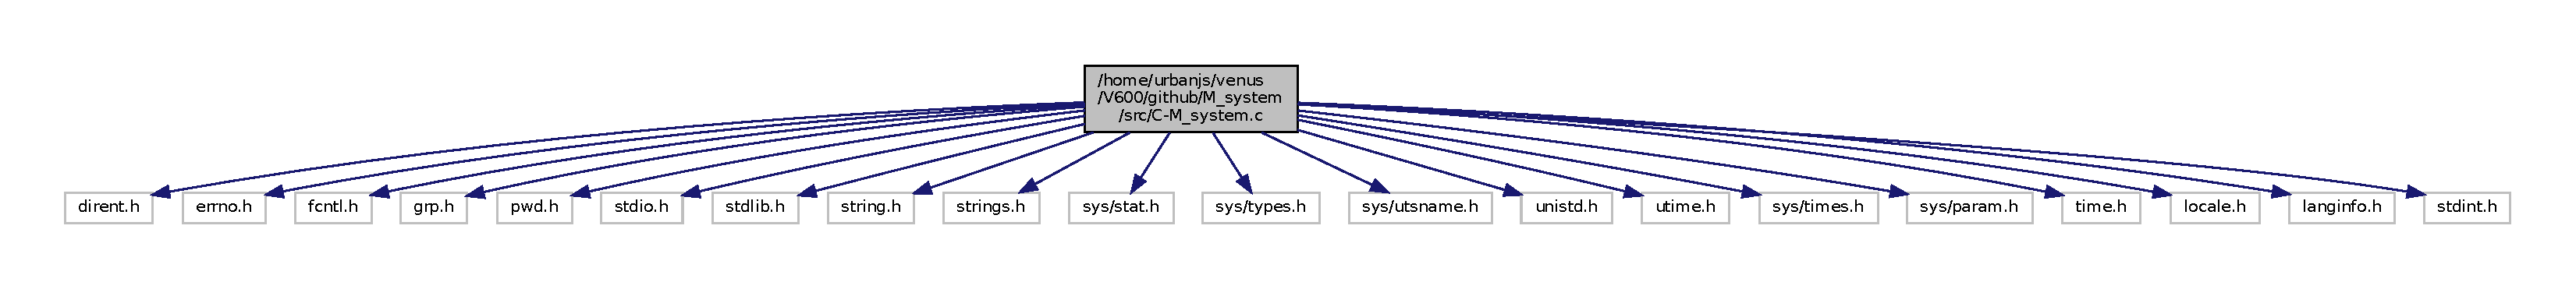
\includegraphics[width=350pt]{C-M__system_8c__incl}
\end{center}
\end{figure}
\subsection*{Macros}
\begin{DoxyCompactItemize}
\item 
\#define \mbox{\hyperlink{C-M__system_8c_a74e75242132eaabbc1c512488a135926}{M\+IN}}(x,  y)~((x) $<$ (y) ? (x) \+: (y))
\end{DoxyCompactItemize}
\subsection*{Functions}
\begin{DoxyCompactItemize}
\item 
int \mbox{\hyperlink{C-M__system_8c_addd32f6d9fc61aa873507167956ac235}{my\+\_\+access}} (const char $\ast$pathname, int which)
\item 
void \mbox{\hyperlink{C-M__system_8c_a21b228b36ba6064c95e68c484f92eaf8}{my\+\_\+mkdir}} (char $\ast$dir, int mode, int $\ast$ier)
\item 
int \mbox{\hyperlink{C-M__system_8c_a5dcb7268b2fb47e193fc6bb9519c6ae6}{my\+\_\+utime}} (const char $\ast$file, int times\mbox{[}2\mbox{]})
\item 
int \mbox{\hyperlink{C-M__system_8c_acfa12de4342c03519fc35d7892db94b2}{my\+\_\+chown}} (char $\ast$filename, long long int uid, long long int gid)
\item 
void \mbox{\hyperlink{C-M__system_8c_a91bcacc76b5a33845775f92e9608ac9c}{my\+\_\+readdir}} (D\+IR $\ast$dirp, char $\ast$filename, int $\ast$ierr)
\item 
void \mbox{\hyperlink{C-M__system_8c_aaf9088f4cc3498dcf1abec624adabe76}{my\+\_\+flush}} (void)
\item 
char $\ast$ \mbox{\hyperlink{C-M__system_8c_a3cdda415df9f1522e545474e11c78a5c}{my\+\_\+realpath}} (char $\ast$symlinkpath)
\item 
void \mbox{\hyperlink{C-M__system_8c_ab5188f2ca99719a14c77a1acae06f93a}{my\+\_\+initenv}} ()
\item 
void \mbox{\hyperlink{C-M__system_8c_a0114eece06797ba0c5e6f5948841501a}{my\+\_\+readenv}} (char $\ast$variable)
\item 
int \mbox{\hyperlink{C-M__system_8c_a13b282e9de0dc0bb29bec1d76aaf6cf0}{my\+\_\+getgrgid}} (long long int id, char $\ast$groupname)
\item 
int \mbox{\hyperlink{C-M__system_8c_a0feb597a044e16699952e0056390f3d6}{my\+\_\+getpwuid}} (long long int id, char $\ast$username)
\item 
int \mbox{\hyperlink{C-M__system_8c_ad9bbaffdef223d18bb59a22c3c599201}{my\+\_\+errno}} ()
\item 
void \mbox{\hyperlink{C-M__system_8c_ab955d6c562df08b9e465fe3cea24d83d}{system\+\_\+unbuffer}} ()
\item 
void \mbox{\hyperlink{C-M__system_8c_ab341d42a9117c4bd188dcdcbff69fe9a}{my\+\_\+uname}} (char $\ast$which, char $\ast$string, int $\ast$stringlen)
\item 
void \mbox{\hyperlink{C-M__system_8c_aae18c27a21f7c4aed7328460a7edb34c}{my\+\_\+cpu\+\_\+time}} (float $\ast$c, float $\ast$u, float $\ast$s)
\item 
int \mbox{\hyperlink{C-M__system_8c_a4d9118bb9590e12ac1956789cd08e09b}{my\+\_\+isdir}} (const char $\ast$path)
\item 
int \mbox{\hyperlink{C-M__system_8c_afec6872f4aa34aba9e71a18324d53bce}{my\+\_\+isreg}} (const char $\ast$path)
\item 
int \mbox{\hyperlink{C-M__system_8c_ad07b549d969a0670b0b8f7c6bef83e92}{my\+\_\+isblk}} (const char $\ast$path)
\item 
int \mbox{\hyperlink{C-M__system_8c_ae59ec13b3517e84ddd30a0cd5352a01d}{my\+\_\+ischr}} (const char $\ast$path)
\item 
int \mbox{\hyperlink{C-M__system_8c_ac4f0c51cc048efce7cc88a80c6ce50a4}{my\+\_\+isfifo}} (const char $\ast$path)
\item 
int \mbox{\hyperlink{C-M__system_8c_a090bd041de7e5661c0cb3dea61517283}{my\+\_\+issock}} (const char $\ast$path)
\item 
int \mbox{\hyperlink{C-M__system_8c_a5d15b99bbdd2c6d3e07c92b4bdebb732}{my\+\_\+islnk}} (const char $\ast$fname)
\item 
int \mbox{\hyperlink{C-M__system_8c_afc05a3ec2be734d741c384e752f96b90}{my\+\_\+file\+\_\+exists}} (const char $\ast$fname)
\item 
void \mbox{\hyperlink{C-M__system_8c_a93aa717690d60568cf019988f6434ba5}{my\+\_\+stat}} (char $\ast$file, long int $\ast$values, int $\ast$ierr, int debug)
\item 
const char $\ast$ \mbox{\hyperlink{C-M__system_8c_a1ef2ab1c7375f6b130cee762e770a29a}{my\+\_\+get\+\_\+perm}} (long int imode)
\item 
char \mbox{\hyperlink{C-M__system_8c_a00682f21b3d8ff5bbe69bf47e00f60ab}{getkeyC}} (void)
\item 
int \mbox{\hyperlink{C-M__system_8c_a834a89f46bdca2fc961db64cf3112cdf}{putkeyC}} (char c)
\end{DoxyCompactItemize}
\subsection*{Variables}
\begin{DoxyCompactItemize}
\item 
char $\ast$$\ast$ \mbox{\hyperlink{C-M__system_8c_aa006daaf11f1e2e45a6ababaf463212b}{environ}}
\item 
int \mbox{\hyperlink{C-M__system_8c_a55fec1e650e6037d352db493bea1716f}{F\+H\+O\+S\+T\+\_\+\+N\+A\+M\+E\+\_\+\+M\+AX}} =H\+O\+S\+T\+\_\+\+N\+A\+M\+E\+\_\+\+M\+AX
\item 
mode\+\_\+t \mbox{\hyperlink{C-M__system_8c_a9e37e108fa1a58b85031aed8634f65d0}{F\+S\+\_\+\+I\+R\+G\+RP}} =S\+\_\+\+I\+R\+G\+RP
\item 
mode\+\_\+t \mbox{\hyperlink{C-M__system_8c_a310094a449c3371ef9cf8b0776213835}{F\+S\+\_\+\+I\+R\+O\+TH}} =S\+\_\+\+I\+R\+O\+TH
\item 
mode\+\_\+t \mbox{\hyperlink{C-M__system_8c_a03e3496451f60edd6c69c3802e11db67}{F\+S\+\_\+\+I\+R\+U\+SR}} =S\+\_\+\+I\+R\+U\+SR
\item 
mode\+\_\+t \mbox{\hyperlink{C-M__system_8c_ab4e744ca243de9628a7e9651695d7a97}{F\+S\+\_\+\+I\+R\+W\+XG}} =S\+\_\+\+I\+R\+W\+XG
\item 
mode\+\_\+t \mbox{\hyperlink{C-M__system_8c_a612adf3e64ccb1734ab64ef6d73fa87b}{F\+S\+\_\+\+I\+R\+W\+XO}} =S\+\_\+\+I\+R\+W\+XO
\item 
mode\+\_\+t \mbox{\hyperlink{C-M__system_8c_acb420eb45e494ab53bbfd018c2262ff2}{F\+S\+\_\+\+I\+R\+W\+XU}} =S\+\_\+\+I\+R\+W\+XU
\item 
mode\+\_\+t \mbox{\hyperlink{C-M__system_8c_a739522a271fd37727d6f266197ded32b}{F\+S\+\_\+\+I\+W\+G\+RP}} =S\+\_\+\+I\+W\+G\+RP
\item 
mode\+\_\+t \mbox{\hyperlink{C-M__system_8c_a1ed0df6f1e0108d07c0fe7880402f8c0}{F\+S\+\_\+\+I\+W\+O\+TH}} =S\+\_\+\+I\+W\+O\+TH
\item 
mode\+\_\+t \mbox{\hyperlink{C-M__system_8c_ade549697e7611d5c3755b1befcd796b8}{F\+S\+\_\+\+I\+W\+U\+SR}} =S\+\_\+\+I\+W\+U\+SR
\item 
mode\+\_\+t \mbox{\hyperlink{C-M__system_8c_ac01832589f29b7d987cb90be63cc3dc8}{F\+S\+\_\+\+I\+X\+G\+RP}} =S\+\_\+\+I\+X\+G\+RP
\item 
mode\+\_\+t \mbox{\hyperlink{C-M__system_8c_aafbcf1020ef1a8f3999526f88f349fe3}{F\+S\+\_\+\+I\+X\+O\+TH}} =S\+\_\+\+I\+X\+O\+TH
\item 
mode\+\_\+t \mbox{\hyperlink{C-M__system_8c_acc949c15ea63678fc34579213919906f}{F\+S\+\_\+\+I\+X\+U\+SR}} =S\+\_\+\+I\+X\+U\+SR
\item 
mode\+\_\+t \mbox{\hyperlink{C-M__system_8c_a4ec9ddefca39a5f2bc0aa0cb9cc8a760}{F\+D\+E\+F\+F\+I\+L\+E\+M\+O\+DE}} =D\+E\+F\+F\+I\+L\+E\+M\+O\+DE
\item 
mode\+\_\+t \mbox{\hyperlink{C-M__system_8c_a2d221d0dde92c4e100c2bc959832f1df}{F\+A\+C\+C\+E\+S\+S\+P\+E\+R\+MS}} =A\+C\+C\+E\+S\+S\+P\+E\+R\+MS
\item 
char $\ast$$\ast$ \mbox{\hyperlink{C-M__system_8c_a8f6f268f0282f4a41c1569e80963f328}{ep}}
\item 
long int \mbox{\hyperlink{C-M__system_8c_ad45ba6068349b626136d161ff72dea21}{longest\+\_\+env\+\_\+variable}} =0L
\end{DoxyCompactItemize}


\subsection{Macro Definition Documentation}
\mbox{\Hypertarget{C-M__system_8c_a74e75242132eaabbc1c512488a135926}\label{C-M__system_8c_a74e75242132eaabbc1c512488a135926}} 
\index{C-\/\+M\+\_\+system.\+c@{C-\/\+M\+\_\+system.\+c}!M\+IN@{M\+IN}}
\index{M\+IN@{M\+IN}!C-\/\+M\+\_\+system.\+c@{C-\/\+M\+\_\+system.\+c}}
\subsubsection{\texorpdfstring{M\+IN}{MIN}}
{\footnotesize\ttfamily \#define M\+IN(\begin{DoxyParamCaption}\item[{}]{x,  }\item[{}]{y }\end{DoxyParamCaption})~((x) $<$ (y) ? (x) \+: (y))}



\subsection{Function Documentation}
\mbox{\Hypertarget{C-M__system_8c_a00682f21b3d8ff5bbe69bf47e00f60ab}\label{C-M__system_8c_a00682f21b3d8ff5bbe69bf47e00f60ab}} 
\index{C-\/\+M\+\_\+system.\+c@{C-\/\+M\+\_\+system.\+c}!getkeyC@{getkeyC}}
\index{getkeyC@{getkeyC}!C-\/\+M\+\_\+system.\+c@{C-\/\+M\+\_\+system.\+c}}
\subsubsection{\texorpdfstring{getkey\+C()}{getkeyC()}}
{\footnotesize\ttfamily char getkeyC (\begin{DoxyParamCaption}\item[{void}]{ }\end{DoxyParamCaption})}

\mbox{\Hypertarget{C-M__system_8c_addd32f6d9fc61aa873507167956ac235}\label{C-M__system_8c_addd32f6d9fc61aa873507167956ac235}} 
\index{C-\/\+M\+\_\+system.\+c@{C-\/\+M\+\_\+system.\+c}!my\+\_\+access@{my\+\_\+access}}
\index{my\+\_\+access@{my\+\_\+access}!C-\/\+M\+\_\+system.\+c@{C-\/\+M\+\_\+system.\+c}}
\subsubsection{\texorpdfstring{my\+\_\+access()}{my\_access()}}
{\footnotesize\ttfamily int my\+\_\+access (\begin{DoxyParamCaption}\item[{const char $\ast$}]{pathname,  }\item[{int}]{which }\end{DoxyParamCaption})}

\mbox{\Hypertarget{C-M__system_8c_acfa12de4342c03519fc35d7892db94b2}\label{C-M__system_8c_acfa12de4342c03519fc35d7892db94b2}} 
\index{C-\/\+M\+\_\+system.\+c@{C-\/\+M\+\_\+system.\+c}!my\+\_\+chown@{my\+\_\+chown}}
\index{my\+\_\+chown@{my\+\_\+chown}!C-\/\+M\+\_\+system.\+c@{C-\/\+M\+\_\+system.\+c}}
\subsubsection{\texorpdfstring{my\+\_\+chown()}{my\_chown()}}
{\footnotesize\ttfamily int my\+\_\+chown (\begin{DoxyParamCaption}\item[{char $\ast$}]{filename,  }\item[{long long int}]{uid,  }\item[{long long int}]{gid }\end{DoxyParamCaption})}

\mbox{\Hypertarget{C-M__system_8c_aae18c27a21f7c4aed7328460a7edb34c}\label{C-M__system_8c_aae18c27a21f7c4aed7328460a7edb34c}} 
\index{C-\/\+M\+\_\+system.\+c@{C-\/\+M\+\_\+system.\+c}!my\+\_\+cpu\+\_\+time@{my\+\_\+cpu\+\_\+time}}
\index{my\+\_\+cpu\+\_\+time@{my\+\_\+cpu\+\_\+time}!C-\/\+M\+\_\+system.\+c@{C-\/\+M\+\_\+system.\+c}}
\subsubsection{\texorpdfstring{my\+\_\+cpu\+\_\+time()}{my\_cpu\_time()}}
{\footnotesize\ttfamily void my\+\_\+cpu\+\_\+time (\begin{DoxyParamCaption}\item[{float $\ast$}]{c,  }\item[{float $\ast$}]{u,  }\item[{float $\ast$}]{s }\end{DoxyParamCaption})}

\mbox{\Hypertarget{C-M__system_8c_ad9bbaffdef223d18bb59a22c3c599201}\label{C-M__system_8c_ad9bbaffdef223d18bb59a22c3c599201}} 
\index{C-\/\+M\+\_\+system.\+c@{C-\/\+M\+\_\+system.\+c}!my\+\_\+errno@{my\+\_\+errno}}
\index{my\+\_\+errno@{my\+\_\+errno}!C-\/\+M\+\_\+system.\+c@{C-\/\+M\+\_\+system.\+c}}
\subsubsection{\texorpdfstring{my\+\_\+errno()}{my\_errno()}}
{\footnotesize\ttfamily int my\+\_\+errno (\begin{DoxyParamCaption}{ }\end{DoxyParamCaption})}

\mbox{\Hypertarget{C-M__system_8c_afc05a3ec2be734d741c384e752f96b90}\label{C-M__system_8c_afc05a3ec2be734d741c384e752f96b90}} 
\index{C-\/\+M\+\_\+system.\+c@{C-\/\+M\+\_\+system.\+c}!my\+\_\+file\+\_\+exists@{my\+\_\+file\+\_\+exists}}
\index{my\+\_\+file\+\_\+exists@{my\+\_\+file\+\_\+exists}!C-\/\+M\+\_\+system.\+c@{C-\/\+M\+\_\+system.\+c}}
\subsubsection{\texorpdfstring{my\+\_\+file\+\_\+exists()}{my\_file\_exists()}}
{\footnotesize\ttfamily int my\+\_\+file\+\_\+exists (\begin{DoxyParamCaption}\item[{const char $\ast$}]{fname }\end{DoxyParamCaption})}

\mbox{\Hypertarget{C-M__system_8c_aaf9088f4cc3498dcf1abec624adabe76}\label{C-M__system_8c_aaf9088f4cc3498dcf1abec624adabe76}} 
\index{C-\/\+M\+\_\+system.\+c@{C-\/\+M\+\_\+system.\+c}!my\+\_\+flush@{my\+\_\+flush}}
\index{my\+\_\+flush@{my\+\_\+flush}!C-\/\+M\+\_\+system.\+c@{C-\/\+M\+\_\+system.\+c}}
\subsubsection{\texorpdfstring{my\+\_\+flush()}{my\_flush()}}
{\footnotesize\ttfamily void my\+\_\+flush (\begin{DoxyParamCaption}\item[{void}]{ }\end{DoxyParamCaption})}

\mbox{\Hypertarget{C-M__system_8c_a1ef2ab1c7375f6b130cee762e770a29a}\label{C-M__system_8c_a1ef2ab1c7375f6b130cee762e770a29a}} 
\index{C-\/\+M\+\_\+system.\+c@{C-\/\+M\+\_\+system.\+c}!my\+\_\+get\+\_\+perm@{my\+\_\+get\+\_\+perm}}
\index{my\+\_\+get\+\_\+perm@{my\+\_\+get\+\_\+perm}!C-\/\+M\+\_\+system.\+c@{C-\/\+M\+\_\+system.\+c}}
\subsubsection{\texorpdfstring{my\+\_\+get\+\_\+perm()}{my\_get\_perm()}}
{\footnotesize\ttfamily const char$\ast$ my\+\_\+get\+\_\+perm (\begin{DoxyParamCaption}\item[{long int}]{imode }\end{DoxyParamCaption})}



References m\+\_\+system\+::mode\+\_\+t.

\mbox{\Hypertarget{C-M__system_8c_a13b282e9de0dc0bb29bec1d76aaf6cf0}\label{C-M__system_8c_a13b282e9de0dc0bb29bec1d76aaf6cf0}} 
\index{C-\/\+M\+\_\+system.\+c@{C-\/\+M\+\_\+system.\+c}!my\+\_\+getgrgid@{my\+\_\+getgrgid}}
\index{my\+\_\+getgrgid@{my\+\_\+getgrgid}!C-\/\+M\+\_\+system.\+c@{C-\/\+M\+\_\+system.\+c}}
\subsubsection{\texorpdfstring{my\+\_\+getgrgid()}{my\_getgrgid()}}
{\footnotesize\ttfamily int my\+\_\+getgrgid (\begin{DoxyParamCaption}\item[{long long int}]{id,  }\item[{char $\ast$}]{groupname }\end{DoxyParamCaption})}

\mbox{\Hypertarget{C-M__system_8c_a0feb597a044e16699952e0056390f3d6}\label{C-M__system_8c_a0feb597a044e16699952e0056390f3d6}} 
\index{C-\/\+M\+\_\+system.\+c@{C-\/\+M\+\_\+system.\+c}!my\+\_\+getpwuid@{my\+\_\+getpwuid}}
\index{my\+\_\+getpwuid@{my\+\_\+getpwuid}!C-\/\+M\+\_\+system.\+c@{C-\/\+M\+\_\+system.\+c}}
\subsubsection{\texorpdfstring{my\+\_\+getpwuid()}{my\_getpwuid()}}
{\footnotesize\ttfamily int my\+\_\+getpwuid (\begin{DoxyParamCaption}\item[{long long int}]{id,  }\item[{char $\ast$}]{username }\end{DoxyParamCaption})}

\mbox{\Hypertarget{C-M__system_8c_ab5188f2ca99719a14c77a1acae06f93a}\label{C-M__system_8c_ab5188f2ca99719a14c77a1acae06f93a}} 
\index{C-\/\+M\+\_\+system.\+c@{C-\/\+M\+\_\+system.\+c}!my\+\_\+initenv@{my\+\_\+initenv}}
\index{my\+\_\+initenv@{my\+\_\+initenv}!C-\/\+M\+\_\+system.\+c@{C-\/\+M\+\_\+system.\+c}}
\subsubsection{\texorpdfstring{my\+\_\+initenv()}{my\_initenv()}}
{\footnotesize\ttfamily void my\+\_\+initenv (\begin{DoxyParamCaption}{ }\end{DoxyParamCaption})}



References environ, ep, and longest\+\_\+env\+\_\+variable.

Here is the caller graph for this function\+:\nopagebreak
\begin{figure}[H]
\begin{center}
\leavevmode
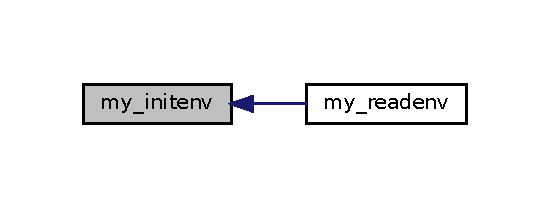
\includegraphics[width=264pt]{C-M__system_8c_ab5188f2ca99719a14c77a1acae06f93a_icgraph}
\end{center}
\end{figure}
\mbox{\Hypertarget{C-M__system_8c_ad07b549d969a0670b0b8f7c6bef83e92}\label{C-M__system_8c_ad07b549d969a0670b0b8f7c6bef83e92}} 
\index{C-\/\+M\+\_\+system.\+c@{C-\/\+M\+\_\+system.\+c}!my\+\_\+isblk@{my\+\_\+isblk}}
\index{my\+\_\+isblk@{my\+\_\+isblk}!C-\/\+M\+\_\+system.\+c@{C-\/\+M\+\_\+system.\+c}}
\subsubsection{\texorpdfstring{my\+\_\+isblk()}{my\_isblk()}}
{\footnotesize\ttfamily int my\+\_\+isblk (\begin{DoxyParamCaption}\item[{const char $\ast$}]{path }\end{DoxyParamCaption})}

\mbox{\Hypertarget{C-M__system_8c_ae59ec13b3517e84ddd30a0cd5352a01d}\label{C-M__system_8c_ae59ec13b3517e84ddd30a0cd5352a01d}} 
\index{C-\/\+M\+\_\+system.\+c@{C-\/\+M\+\_\+system.\+c}!my\+\_\+ischr@{my\+\_\+ischr}}
\index{my\+\_\+ischr@{my\+\_\+ischr}!C-\/\+M\+\_\+system.\+c@{C-\/\+M\+\_\+system.\+c}}
\subsubsection{\texorpdfstring{my\+\_\+ischr()}{my\_ischr()}}
{\footnotesize\ttfamily int my\+\_\+ischr (\begin{DoxyParamCaption}\item[{const char $\ast$}]{path }\end{DoxyParamCaption})}

\mbox{\Hypertarget{C-M__system_8c_a4d9118bb9590e12ac1956789cd08e09b}\label{C-M__system_8c_a4d9118bb9590e12ac1956789cd08e09b}} 
\index{C-\/\+M\+\_\+system.\+c@{C-\/\+M\+\_\+system.\+c}!my\+\_\+isdir@{my\+\_\+isdir}}
\index{my\+\_\+isdir@{my\+\_\+isdir}!C-\/\+M\+\_\+system.\+c@{C-\/\+M\+\_\+system.\+c}}
\subsubsection{\texorpdfstring{my\+\_\+isdir()}{my\_isdir()}}
{\footnotesize\ttfamily int my\+\_\+isdir (\begin{DoxyParamCaption}\item[{const char $\ast$}]{path }\end{DoxyParamCaption})}

\mbox{\Hypertarget{C-M__system_8c_ac4f0c51cc048efce7cc88a80c6ce50a4}\label{C-M__system_8c_ac4f0c51cc048efce7cc88a80c6ce50a4}} 
\index{C-\/\+M\+\_\+system.\+c@{C-\/\+M\+\_\+system.\+c}!my\+\_\+isfifo@{my\+\_\+isfifo}}
\index{my\+\_\+isfifo@{my\+\_\+isfifo}!C-\/\+M\+\_\+system.\+c@{C-\/\+M\+\_\+system.\+c}}
\subsubsection{\texorpdfstring{my\+\_\+isfifo()}{my\_isfifo()}}
{\footnotesize\ttfamily int my\+\_\+isfifo (\begin{DoxyParamCaption}\item[{const char $\ast$}]{path }\end{DoxyParamCaption})}

\mbox{\Hypertarget{C-M__system_8c_a5d15b99bbdd2c6d3e07c92b4bdebb732}\label{C-M__system_8c_a5d15b99bbdd2c6d3e07c92b4bdebb732}} 
\index{C-\/\+M\+\_\+system.\+c@{C-\/\+M\+\_\+system.\+c}!my\+\_\+islnk@{my\+\_\+islnk}}
\index{my\+\_\+islnk@{my\+\_\+islnk}!C-\/\+M\+\_\+system.\+c@{C-\/\+M\+\_\+system.\+c}}
\subsubsection{\texorpdfstring{my\+\_\+islnk()}{my\_islnk()}}
{\footnotesize\ttfamily int my\+\_\+islnk (\begin{DoxyParamCaption}\item[{const char $\ast$}]{fname }\end{DoxyParamCaption})}

\mbox{\Hypertarget{C-M__system_8c_afec6872f4aa34aba9e71a18324d53bce}\label{C-M__system_8c_afec6872f4aa34aba9e71a18324d53bce}} 
\index{C-\/\+M\+\_\+system.\+c@{C-\/\+M\+\_\+system.\+c}!my\+\_\+isreg@{my\+\_\+isreg}}
\index{my\+\_\+isreg@{my\+\_\+isreg}!C-\/\+M\+\_\+system.\+c@{C-\/\+M\+\_\+system.\+c}}
\subsubsection{\texorpdfstring{my\+\_\+isreg()}{my\_isreg()}}
{\footnotesize\ttfamily int my\+\_\+isreg (\begin{DoxyParamCaption}\item[{const char $\ast$}]{path }\end{DoxyParamCaption})}

\mbox{\Hypertarget{C-M__system_8c_a090bd041de7e5661c0cb3dea61517283}\label{C-M__system_8c_a090bd041de7e5661c0cb3dea61517283}} 
\index{C-\/\+M\+\_\+system.\+c@{C-\/\+M\+\_\+system.\+c}!my\+\_\+issock@{my\+\_\+issock}}
\index{my\+\_\+issock@{my\+\_\+issock}!C-\/\+M\+\_\+system.\+c@{C-\/\+M\+\_\+system.\+c}}
\subsubsection{\texorpdfstring{my\+\_\+issock()}{my\_issock()}}
{\footnotesize\ttfamily int my\+\_\+issock (\begin{DoxyParamCaption}\item[{const char $\ast$}]{path }\end{DoxyParamCaption})}

\mbox{\Hypertarget{C-M__system_8c_a21b228b36ba6064c95e68c484f92eaf8}\label{C-M__system_8c_a21b228b36ba6064c95e68c484f92eaf8}} 
\index{C-\/\+M\+\_\+system.\+c@{C-\/\+M\+\_\+system.\+c}!my\+\_\+mkdir@{my\+\_\+mkdir}}
\index{my\+\_\+mkdir@{my\+\_\+mkdir}!C-\/\+M\+\_\+system.\+c@{C-\/\+M\+\_\+system.\+c}}
\subsubsection{\texorpdfstring{my\+\_\+mkdir()}{my\_mkdir()}}
{\footnotesize\ttfamily void my\+\_\+mkdir (\begin{DoxyParamCaption}\item[{char $\ast$}]{dir,  }\item[{int}]{mode,  }\item[{int $\ast$}]{ier }\end{DoxyParamCaption})}

Here is the caller graph for this function\+:
\nopagebreak
\begin{figure}[H]
\begin{center}
\leavevmode
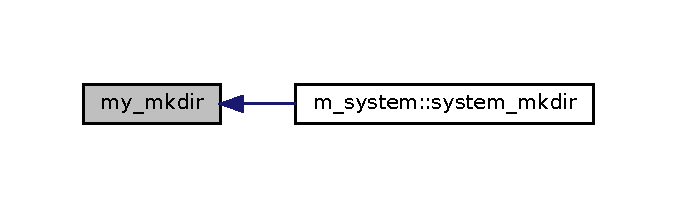
\includegraphics[width=325pt]{C-M__system_8c_a21b228b36ba6064c95e68c484f92eaf8_icgraph}
\end{center}
\end{figure}
\mbox{\Hypertarget{C-M__system_8c_a91bcacc76b5a33845775f92e9608ac9c}\label{C-M__system_8c_a91bcacc76b5a33845775f92e9608ac9c}} 
\index{C-\/\+M\+\_\+system.\+c@{C-\/\+M\+\_\+system.\+c}!my\+\_\+readdir@{my\+\_\+readdir}}
\index{my\+\_\+readdir@{my\+\_\+readdir}!C-\/\+M\+\_\+system.\+c@{C-\/\+M\+\_\+system.\+c}}
\subsubsection{\texorpdfstring{my\+\_\+readdir()}{my\_readdir()}}
{\footnotesize\ttfamily void my\+\_\+readdir (\begin{DoxyParamCaption}\item[{D\+IR $\ast$}]{dirp,  }\item[{char $\ast$}]{filename,  }\item[{int $\ast$}]{ierr }\end{DoxyParamCaption})}

\mbox{\Hypertarget{C-M__system_8c_a0114eece06797ba0c5e6f5948841501a}\label{C-M__system_8c_a0114eece06797ba0c5e6f5948841501a}} 
\index{C-\/\+M\+\_\+system.\+c@{C-\/\+M\+\_\+system.\+c}!my\+\_\+readenv@{my\+\_\+readenv}}
\index{my\+\_\+readenv@{my\+\_\+readenv}!C-\/\+M\+\_\+system.\+c@{C-\/\+M\+\_\+system.\+c}}
\subsubsection{\texorpdfstring{my\+\_\+readenv()}{my\_readenv()}}
{\footnotesize\ttfamily void my\+\_\+readenv (\begin{DoxyParamCaption}\item[{char $\ast$}]{variable }\end{DoxyParamCaption})}



References ep, M\+IN, and my\+\_\+initenv().

Here is the call graph for this function\+:\nopagebreak
\begin{figure}[H]
\begin{center}
\leavevmode
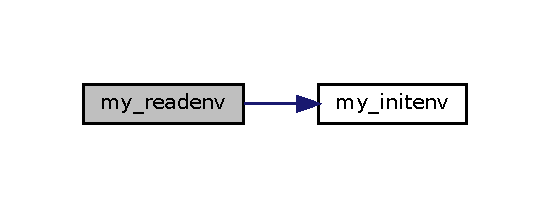
\includegraphics[width=264pt]{C-M__system_8c_a0114eece06797ba0c5e6f5948841501a_cgraph}
\end{center}
\end{figure}
\mbox{\Hypertarget{C-M__system_8c_a3cdda415df9f1522e545474e11c78a5c}\label{C-M__system_8c_a3cdda415df9f1522e545474e11c78a5c}} 
\index{C-\/\+M\+\_\+system.\+c@{C-\/\+M\+\_\+system.\+c}!my\+\_\+realpath@{my\+\_\+realpath}}
\index{my\+\_\+realpath@{my\+\_\+realpath}!C-\/\+M\+\_\+system.\+c@{C-\/\+M\+\_\+system.\+c}}
\subsubsection{\texorpdfstring{my\+\_\+realpath()}{my\_realpath()}}
{\footnotesize\ttfamily char$\ast$ my\+\_\+realpath (\begin{DoxyParamCaption}\item[{char $\ast$}]{symlinkpath }\end{DoxyParamCaption})}

\mbox{\Hypertarget{C-M__system_8c_a93aa717690d60568cf019988f6434ba5}\label{C-M__system_8c_a93aa717690d60568cf019988f6434ba5}} 
\index{C-\/\+M\+\_\+system.\+c@{C-\/\+M\+\_\+system.\+c}!my\+\_\+stat@{my\+\_\+stat}}
\index{my\+\_\+stat@{my\+\_\+stat}!C-\/\+M\+\_\+system.\+c@{C-\/\+M\+\_\+system.\+c}}
\subsubsection{\texorpdfstring{my\+\_\+stat()}{my\_stat()}}
{\footnotesize\ttfamily void my\+\_\+stat (\begin{DoxyParamCaption}\item[{char $\ast$}]{file,  }\item[{long int $\ast$}]{values,  }\item[{int $\ast$}]{ierr,  }\item[{int}]{debug }\end{DoxyParamCaption})}

\mbox{\Hypertarget{C-M__system_8c_ab341d42a9117c4bd188dcdcbff69fe9a}\label{C-M__system_8c_ab341d42a9117c4bd188dcdcbff69fe9a}} 
\index{C-\/\+M\+\_\+system.\+c@{C-\/\+M\+\_\+system.\+c}!my\+\_\+uname@{my\+\_\+uname}}
\index{my\+\_\+uname@{my\+\_\+uname}!C-\/\+M\+\_\+system.\+c@{C-\/\+M\+\_\+system.\+c}}
\subsubsection{\texorpdfstring{my\+\_\+uname()}{my\_uname()}}
{\footnotesize\ttfamily void my\+\_\+uname (\begin{DoxyParamCaption}\item[{char $\ast$}]{which,  }\item[{char $\ast$}]{string,  }\item[{int $\ast$}]{stringlen }\end{DoxyParamCaption})}

\mbox{\Hypertarget{C-M__system_8c_a5dcb7268b2fb47e193fc6bb9519c6ae6}\label{C-M__system_8c_a5dcb7268b2fb47e193fc6bb9519c6ae6}} 
\index{C-\/\+M\+\_\+system.\+c@{C-\/\+M\+\_\+system.\+c}!my\+\_\+utime@{my\+\_\+utime}}
\index{my\+\_\+utime@{my\+\_\+utime}!C-\/\+M\+\_\+system.\+c@{C-\/\+M\+\_\+system.\+c}}
\subsubsection{\texorpdfstring{my\+\_\+utime()}{my\_utime()}}
{\footnotesize\ttfamily int my\+\_\+utime (\begin{DoxyParamCaption}\item[{const char $\ast$}]{file,  }\item[{int}]{times\mbox{[}2\mbox{]} }\end{DoxyParamCaption})}

\mbox{\Hypertarget{C-M__system_8c_a834a89f46bdca2fc961db64cf3112cdf}\label{C-M__system_8c_a834a89f46bdca2fc961db64cf3112cdf}} 
\index{C-\/\+M\+\_\+system.\+c@{C-\/\+M\+\_\+system.\+c}!putkeyC@{putkeyC}}
\index{putkeyC@{putkeyC}!C-\/\+M\+\_\+system.\+c@{C-\/\+M\+\_\+system.\+c}}
\subsubsection{\texorpdfstring{putkey\+C()}{putkeyC()}}
{\footnotesize\ttfamily int putkeyC (\begin{DoxyParamCaption}\item[{char}]{c }\end{DoxyParamCaption})}

\mbox{\Hypertarget{C-M__system_8c_ab955d6c562df08b9e465fe3cea24d83d}\label{C-M__system_8c_ab955d6c562df08b9e465fe3cea24d83d}} 
\index{C-\/\+M\+\_\+system.\+c@{C-\/\+M\+\_\+system.\+c}!system\+\_\+unbuffer@{system\+\_\+unbuffer}}
\index{system\+\_\+unbuffer@{system\+\_\+unbuffer}!C-\/\+M\+\_\+system.\+c@{C-\/\+M\+\_\+system.\+c}}
\subsubsection{\texorpdfstring{system\+\_\+unbuffer()}{system\_unbuffer()}}
{\footnotesize\ttfamily void system\+\_\+unbuffer (\begin{DoxyParamCaption}{ }\end{DoxyParamCaption})}



\subsection{Variable Documentation}
\mbox{\Hypertarget{C-M__system_8c_aa006daaf11f1e2e45a6ababaf463212b}\label{C-M__system_8c_aa006daaf11f1e2e45a6ababaf463212b}} 
\index{C-\/\+M\+\_\+system.\+c@{C-\/\+M\+\_\+system.\+c}!environ@{environ}}
\index{environ@{environ}!C-\/\+M\+\_\+system.\+c@{C-\/\+M\+\_\+system.\+c}}
\subsubsection{\texorpdfstring{environ}{environ}}
{\footnotesize\ttfamily char$\ast$$\ast$ environ}

\mbox{\Hypertarget{C-M__system_8c_a8f6f268f0282f4a41c1569e80963f328}\label{C-M__system_8c_a8f6f268f0282f4a41c1569e80963f328}} 
\index{C-\/\+M\+\_\+system.\+c@{C-\/\+M\+\_\+system.\+c}!ep@{ep}}
\index{ep@{ep}!C-\/\+M\+\_\+system.\+c@{C-\/\+M\+\_\+system.\+c}}
\subsubsection{\texorpdfstring{ep}{ep}}
{\footnotesize\ttfamily char$\ast$$\ast$ ep}

\mbox{\Hypertarget{C-M__system_8c_a2d221d0dde92c4e100c2bc959832f1df}\label{C-M__system_8c_a2d221d0dde92c4e100c2bc959832f1df}} 
\index{C-\/\+M\+\_\+system.\+c@{C-\/\+M\+\_\+system.\+c}!F\+A\+C\+C\+E\+S\+S\+P\+E\+R\+MS@{F\+A\+C\+C\+E\+S\+S\+P\+E\+R\+MS}}
\index{F\+A\+C\+C\+E\+S\+S\+P\+E\+R\+MS@{F\+A\+C\+C\+E\+S\+S\+P\+E\+R\+MS}!C-\/\+M\+\_\+system.\+c@{C-\/\+M\+\_\+system.\+c}}
\subsubsection{\texorpdfstring{F\+A\+C\+C\+E\+S\+S\+P\+E\+R\+MS}{FACCESSPERMS}}
{\footnotesize\ttfamily mode\+\_\+t F\+A\+C\+C\+E\+S\+S\+P\+E\+R\+MS =A\+C\+C\+E\+S\+S\+P\+E\+R\+MS}

\mbox{\Hypertarget{C-M__system_8c_a4ec9ddefca39a5f2bc0aa0cb9cc8a760}\label{C-M__system_8c_a4ec9ddefca39a5f2bc0aa0cb9cc8a760}} 
\index{C-\/\+M\+\_\+system.\+c@{C-\/\+M\+\_\+system.\+c}!F\+D\+E\+F\+F\+I\+L\+E\+M\+O\+DE@{F\+D\+E\+F\+F\+I\+L\+E\+M\+O\+DE}}
\index{F\+D\+E\+F\+F\+I\+L\+E\+M\+O\+DE@{F\+D\+E\+F\+F\+I\+L\+E\+M\+O\+DE}!C-\/\+M\+\_\+system.\+c@{C-\/\+M\+\_\+system.\+c}}
\subsubsection{\texorpdfstring{F\+D\+E\+F\+F\+I\+L\+E\+M\+O\+DE}{FDEFFILEMODE}}
{\footnotesize\ttfamily mode\+\_\+t F\+D\+E\+F\+F\+I\+L\+E\+M\+O\+DE =D\+E\+F\+F\+I\+L\+E\+M\+O\+DE}

\mbox{\Hypertarget{C-M__system_8c_a55fec1e650e6037d352db493bea1716f}\label{C-M__system_8c_a55fec1e650e6037d352db493bea1716f}} 
\index{C-\/\+M\+\_\+system.\+c@{C-\/\+M\+\_\+system.\+c}!F\+H\+O\+S\+T\+\_\+\+N\+A\+M\+E\+\_\+\+M\+AX@{F\+H\+O\+S\+T\+\_\+\+N\+A\+M\+E\+\_\+\+M\+AX}}
\index{F\+H\+O\+S\+T\+\_\+\+N\+A\+M\+E\+\_\+\+M\+AX@{F\+H\+O\+S\+T\+\_\+\+N\+A\+M\+E\+\_\+\+M\+AX}!C-\/\+M\+\_\+system.\+c@{C-\/\+M\+\_\+system.\+c}}
\subsubsection{\texorpdfstring{F\+H\+O\+S\+T\+\_\+\+N\+A\+M\+E\+\_\+\+M\+AX}{FHOST\_NAME\_MAX}}
{\footnotesize\ttfamily int F\+H\+O\+S\+T\+\_\+\+N\+A\+M\+E\+\_\+\+M\+AX =H\+O\+S\+T\+\_\+\+N\+A\+M\+E\+\_\+\+M\+AX}

\mbox{\Hypertarget{C-M__system_8c_a9e37e108fa1a58b85031aed8634f65d0}\label{C-M__system_8c_a9e37e108fa1a58b85031aed8634f65d0}} 
\index{C-\/\+M\+\_\+system.\+c@{C-\/\+M\+\_\+system.\+c}!F\+S\+\_\+\+I\+R\+G\+RP@{F\+S\+\_\+\+I\+R\+G\+RP}}
\index{F\+S\+\_\+\+I\+R\+G\+RP@{F\+S\+\_\+\+I\+R\+G\+RP}!C-\/\+M\+\_\+system.\+c@{C-\/\+M\+\_\+system.\+c}}
\subsubsection{\texorpdfstring{F\+S\+\_\+\+I\+R\+G\+RP}{FS\_IRGRP}}
{\footnotesize\ttfamily mode\+\_\+t F\+S\+\_\+\+I\+R\+G\+RP =S\+\_\+\+I\+R\+G\+RP}

\mbox{\Hypertarget{C-M__system_8c_a310094a449c3371ef9cf8b0776213835}\label{C-M__system_8c_a310094a449c3371ef9cf8b0776213835}} 
\index{C-\/\+M\+\_\+system.\+c@{C-\/\+M\+\_\+system.\+c}!F\+S\+\_\+\+I\+R\+O\+TH@{F\+S\+\_\+\+I\+R\+O\+TH}}
\index{F\+S\+\_\+\+I\+R\+O\+TH@{F\+S\+\_\+\+I\+R\+O\+TH}!C-\/\+M\+\_\+system.\+c@{C-\/\+M\+\_\+system.\+c}}
\subsubsection{\texorpdfstring{F\+S\+\_\+\+I\+R\+O\+TH}{FS\_IROTH}}
{\footnotesize\ttfamily mode\+\_\+t F\+S\+\_\+\+I\+R\+O\+TH =S\+\_\+\+I\+R\+O\+TH}

\mbox{\Hypertarget{C-M__system_8c_a03e3496451f60edd6c69c3802e11db67}\label{C-M__system_8c_a03e3496451f60edd6c69c3802e11db67}} 
\index{C-\/\+M\+\_\+system.\+c@{C-\/\+M\+\_\+system.\+c}!F\+S\+\_\+\+I\+R\+U\+SR@{F\+S\+\_\+\+I\+R\+U\+SR}}
\index{F\+S\+\_\+\+I\+R\+U\+SR@{F\+S\+\_\+\+I\+R\+U\+SR}!C-\/\+M\+\_\+system.\+c@{C-\/\+M\+\_\+system.\+c}}
\subsubsection{\texorpdfstring{F\+S\+\_\+\+I\+R\+U\+SR}{FS\_IRUSR}}
{\footnotesize\ttfamily mode\+\_\+t F\+S\+\_\+\+I\+R\+U\+SR =S\+\_\+\+I\+R\+U\+SR}

\mbox{\Hypertarget{C-M__system_8c_ab4e744ca243de9628a7e9651695d7a97}\label{C-M__system_8c_ab4e744ca243de9628a7e9651695d7a97}} 
\index{C-\/\+M\+\_\+system.\+c@{C-\/\+M\+\_\+system.\+c}!F\+S\+\_\+\+I\+R\+W\+XG@{F\+S\+\_\+\+I\+R\+W\+XG}}
\index{F\+S\+\_\+\+I\+R\+W\+XG@{F\+S\+\_\+\+I\+R\+W\+XG}!C-\/\+M\+\_\+system.\+c@{C-\/\+M\+\_\+system.\+c}}
\subsubsection{\texorpdfstring{F\+S\+\_\+\+I\+R\+W\+XG}{FS\_IRWXG}}
{\footnotesize\ttfamily mode\+\_\+t F\+S\+\_\+\+I\+R\+W\+XG =S\+\_\+\+I\+R\+W\+XG}

\mbox{\Hypertarget{C-M__system_8c_a612adf3e64ccb1734ab64ef6d73fa87b}\label{C-M__system_8c_a612adf3e64ccb1734ab64ef6d73fa87b}} 
\index{C-\/\+M\+\_\+system.\+c@{C-\/\+M\+\_\+system.\+c}!F\+S\+\_\+\+I\+R\+W\+XO@{F\+S\+\_\+\+I\+R\+W\+XO}}
\index{F\+S\+\_\+\+I\+R\+W\+XO@{F\+S\+\_\+\+I\+R\+W\+XO}!C-\/\+M\+\_\+system.\+c@{C-\/\+M\+\_\+system.\+c}}
\subsubsection{\texorpdfstring{F\+S\+\_\+\+I\+R\+W\+XO}{FS\_IRWXO}}
{\footnotesize\ttfamily mode\+\_\+t F\+S\+\_\+\+I\+R\+W\+XO =S\+\_\+\+I\+R\+W\+XO}

\mbox{\Hypertarget{C-M__system_8c_acb420eb45e494ab53bbfd018c2262ff2}\label{C-M__system_8c_acb420eb45e494ab53bbfd018c2262ff2}} 
\index{C-\/\+M\+\_\+system.\+c@{C-\/\+M\+\_\+system.\+c}!F\+S\+\_\+\+I\+R\+W\+XU@{F\+S\+\_\+\+I\+R\+W\+XU}}
\index{F\+S\+\_\+\+I\+R\+W\+XU@{F\+S\+\_\+\+I\+R\+W\+XU}!C-\/\+M\+\_\+system.\+c@{C-\/\+M\+\_\+system.\+c}}
\subsubsection{\texorpdfstring{F\+S\+\_\+\+I\+R\+W\+XU}{FS\_IRWXU}}
{\footnotesize\ttfamily mode\+\_\+t F\+S\+\_\+\+I\+R\+W\+XU =S\+\_\+\+I\+R\+W\+XU}

\mbox{\Hypertarget{C-M__system_8c_a739522a271fd37727d6f266197ded32b}\label{C-M__system_8c_a739522a271fd37727d6f266197ded32b}} 
\index{C-\/\+M\+\_\+system.\+c@{C-\/\+M\+\_\+system.\+c}!F\+S\+\_\+\+I\+W\+G\+RP@{F\+S\+\_\+\+I\+W\+G\+RP}}
\index{F\+S\+\_\+\+I\+W\+G\+RP@{F\+S\+\_\+\+I\+W\+G\+RP}!C-\/\+M\+\_\+system.\+c@{C-\/\+M\+\_\+system.\+c}}
\subsubsection{\texorpdfstring{F\+S\+\_\+\+I\+W\+G\+RP}{FS\_IWGRP}}
{\footnotesize\ttfamily mode\+\_\+t F\+S\+\_\+\+I\+W\+G\+RP =S\+\_\+\+I\+W\+G\+RP}

\mbox{\Hypertarget{C-M__system_8c_a1ed0df6f1e0108d07c0fe7880402f8c0}\label{C-M__system_8c_a1ed0df6f1e0108d07c0fe7880402f8c0}} 
\index{C-\/\+M\+\_\+system.\+c@{C-\/\+M\+\_\+system.\+c}!F\+S\+\_\+\+I\+W\+O\+TH@{F\+S\+\_\+\+I\+W\+O\+TH}}
\index{F\+S\+\_\+\+I\+W\+O\+TH@{F\+S\+\_\+\+I\+W\+O\+TH}!C-\/\+M\+\_\+system.\+c@{C-\/\+M\+\_\+system.\+c}}
\subsubsection{\texorpdfstring{F\+S\+\_\+\+I\+W\+O\+TH}{FS\_IWOTH}}
{\footnotesize\ttfamily mode\+\_\+t F\+S\+\_\+\+I\+W\+O\+TH =S\+\_\+\+I\+W\+O\+TH}

\mbox{\Hypertarget{C-M__system_8c_ade549697e7611d5c3755b1befcd796b8}\label{C-M__system_8c_ade549697e7611d5c3755b1befcd796b8}} 
\index{C-\/\+M\+\_\+system.\+c@{C-\/\+M\+\_\+system.\+c}!F\+S\+\_\+\+I\+W\+U\+SR@{F\+S\+\_\+\+I\+W\+U\+SR}}
\index{F\+S\+\_\+\+I\+W\+U\+SR@{F\+S\+\_\+\+I\+W\+U\+SR}!C-\/\+M\+\_\+system.\+c@{C-\/\+M\+\_\+system.\+c}}
\subsubsection{\texorpdfstring{F\+S\+\_\+\+I\+W\+U\+SR}{FS\_IWUSR}}
{\footnotesize\ttfamily mode\+\_\+t F\+S\+\_\+\+I\+W\+U\+SR =S\+\_\+\+I\+W\+U\+SR}

\mbox{\Hypertarget{C-M__system_8c_ac01832589f29b7d987cb90be63cc3dc8}\label{C-M__system_8c_ac01832589f29b7d987cb90be63cc3dc8}} 
\index{C-\/\+M\+\_\+system.\+c@{C-\/\+M\+\_\+system.\+c}!F\+S\+\_\+\+I\+X\+G\+RP@{F\+S\+\_\+\+I\+X\+G\+RP}}
\index{F\+S\+\_\+\+I\+X\+G\+RP@{F\+S\+\_\+\+I\+X\+G\+RP}!C-\/\+M\+\_\+system.\+c@{C-\/\+M\+\_\+system.\+c}}
\subsubsection{\texorpdfstring{F\+S\+\_\+\+I\+X\+G\+RP}{FS\_IXGRP}}
{\footnotesize\ttfamily mode\+\_\+t F\+S\+\_\+\+I\+X\+G\+RP =S\+\_\+\+I\+X\+G\+RP}

\mbox{\Hypertarget{C-M__system_8c_aafbcf1020ef1a8f3999526f88f349fe3}\label{C-M__system_8c_aafbcf1020ef1a8f3999526f88f349fe3}} 
\index{C-\/\+M\+\_\+system.\+c@{C-\/\+M\+\_\+system.\+c}!F\+S\+\_\+\+I\+X\+O\+TH@{F\+S\+\_\+\+I\+X\+O\+TH}}
\index{F\+S\+\_\+\+I\+X\+O\+TH@{F\+S\+\_\+\+I\+X\+O\+TH}!C-\/\+M\+\_\+system.\+c@{C-\/\+M\+\_\+system.\+c}}
\subsubsection{\texorpdfstring{F\+S\+\_\+\+I\+X\+O\+TH}{FS\_IXOTH}}
{\footnotesize\ttfamily mode\+\_\+t F\+S\+\_\+\+I\+X\+O\+TH =S\+\_\+\+I\+X\+O\+TH}

\mbox{\Hypertarget{C-M__system_8c_acc949c15ea63678fc34579213919906f}\label{C-M__system_8c_acc949c15ea63678fc34579213919906f}} 
\index{C-\/\+M\+\_\+system.\+c@{C-\/\+M\+\_\+system.\+c}!F\+S\+\_\+\+I\+X\+U\+SR@{F\+S\+\_\+\+I\+X\+U\+SR}}
\index{F\+S\+\_\+\+I\+X\+U\+SR@{F\+S\+\_\+\+I\+X\+U\+SR}!C-\/\+M\+\_\+system.\+c@{C-\/\+M\+\_\+system.\+c}}
\subsubsection{\texorpdfstring{F\+S\+\_\+\+I\+X\+U\+SR}{FS\_IXUSR}}
{\footnotesize\ttfamily mode\+\_\+t F\+S\+\_\+\+I\+X\+U\+SR =S\+\_\+\+I\+X\+U\+SR}

\mbox{\Hypertarget{C-M__system_8c_ad45ba6068349b626136d161ff72dea21}\label{C-M__system_8c_ad45ba6068349b626136d161ff72dea21}} 
\index{C-\/\+M\+\_\+system.\+c@{C-\/\+M\+\_\+system.\+c}!longest\+\_\+env\+\_\+variable@{longest\+\_\+env\+\_\+variable}}
\index{longest\+\_\+env\+\_\+variable@{longest\+\_\+env\+\_\+variable}!C-\/\+M\+\_\+system.\+c@{C-\/\+M\+\_\+system.\+c}}
\subsubsection{\texorpdfstring{longest\+\_\+env\+\_\+variable}{longest\_env\_variable}}
{\footnotesize\ttfamily long int longest\+\_\+env\+\_\+variable =0L}


\hypertarget{M__system_8f90}{}\section{/home/urbanjs/venus/\+V600/github/\+M\+\_\+system/src/\+M\+\_\+system.f90 File Reference}
\label{M__system_8f90}\index{/home/urbanjs/venus/\+V600/github/\+M\+\_\+system/src/\+M\+\_\+system.\+f90@{/home/urbanjs/venus/\+V600/github/\+M\+\_\+system/src/\+M\+\_\+system.\+f90}}
\subsection*{Data Types}
\begin{DoxyCompactItemize}
\item 
type \mbox{\hyperlink{structm__system_1_1dirent__systema}{m\+\_\+system\+::dirent\+\_\+systema}}
\item 
type \mbox{\hyperlink{structm__system_1_1dirent__cygwin}{m\+\_\+system\+::dirent\+\_\+cygwin}}
\item 
interface \mbox{\hyperlink{interfacem__system_1_1system__alarm}{m\+\_\+system\+::system\+\_\+alarm}}
\item 
interface \mbox{\hyperlink{interfacem__system_1_1system__calloc}{m\+\_\+system\+::system\+\_\+calloc}}
\item 
interface \mbox{\hyperlink{interfacem__system_1_1system__clock}{m\+\_\+system\+::system\+\_\+clock}}
\item 
interface \mbox{\hyperlink{interfacem__system_1_1system__memcpy}{m\+\_\+system\+::system\+\_\+memcpy}}
\item 
interface \mbox{\hyperlink{interfacem__system_1_1system__free}{m\+\_\+system\+::system\+\_\+free}}
\item 
interface \mbox{\hyperlink{interfacem__system_1_1system__malloc}{m\+\_\+system\+::system\+\_\+malloc}}
\item 
interface \mbox{\hyperlink{interfacem__system_1_1system__realloc}{m\+\_\+system\+::system\+\_\+realloc}}
\item 
interface \mbox{\hyperlink{interfacem__system_1_1system__time}{m\+\_\+system\+::system\+\_\+time}}
\item 
interface \mbox{\hyperlink{interfacem__system_1_1system__srand}{m\+\_\+system\+::system\+\_\+srand}}
\begin{DoxyCompactList}\small\item\em \subsubsection*{N\+A\+ME}

system\+\_\+srand(3f) -\/ \mbox{[}M\+\_\+system\mbox{]} set seed for pseudo-\/random number generator system\+\_\+rand(3f) (L\+I\+C\+E\+N\+SE\+:PD) \end{DoxyCompactList}\item 
interface \mbox{\hyperlink{interfacem__system_1_1system__kill}{m\+\_\+system\+::system\+\_\+kill}}
\begin{DoxyCompactList}\small\item\em \subsubsection*{N\+A\+ME}

system\+\_\+kill(3f) -\/ \mbox{[}M\+\_\+system\mbox{]} send a signal to a process or a group of processes (L\+I\+C\+E\+N\+SE\+:PD) \end{DoxyCompactList}\item 
interface \mbox{\hyperlink{interfacem__system_1_1system__errno}{m\+\_\+system\+::system\+\_\+errno}}
\begin{DoxyCompactList}\small\item\em \subsubsection*{N\+A\+ME}

system\+\_\+errno(3f) -\/ \mbox{[}M\+\_\+system\mbox{]} C error return value (L\+I\+C\+E\+N\+SE\+:PD) \subsubsection*{S\+Y\+N\+O\+P\+S\+IS}\end{DoxyCompactList}\item 
interface \mbox{\hyperlink{interfacem__system_1_1system__geteuid}{m\+\_\+system\+::system\+\_\+geteuid}}
\begin{DoxyCompactList}\small\item\em \subsubsection*{N\+A\+ME}

system\+\_\+geteuid(3f) -\/ \mbox{[}M\+\_\+system\+:Q\+U\+E\+RY\mbox{]} get effective U\+ID of current process from Fortran by calling geteuid(3c) (L\+I\+C\+E\+N\+SE\+:PD) \subsubsection*{S\+Y\+N\+O\+P\+S\+IS}\end{DoxyCompactList}\item 
interface \mbox{\hyperlink{interfacem__system_1_1system__getuid}{m\+\_\+system\+::system\+\_\+getuid}}
\begin{DoxyCompactList}\small\item\em \subsubsection*{N\+A\+ME}

system\+\_\+getuid(3f) -\/ \mbox{[}M\+\_\+system\+:Q\+U\+E\+RY\mbox{]} get real U\+ID of current process from Fortran by calling getuid(3c) (L\+I\+C\+E\+N\+SE\+:PD) \subsubsection*{S\+Y\+N\+O\+P\+S\+IS}\end{DoxyCompactList}\item 
interface \mbox{\hyperlink{interfacem__system_1_1system__getegid}{m\+\_\+system\+::system\+\_\+getegid}}
\begin{DoxyCompactList}\small\item\em \subsubsection*{N\+A\+ME}

system\+\_\+getegid(3f) -\/ \mbox{[}M\+\_\+system\+:Q\+U\+E\+RY\mbox{]} get the effective group ID (G\+ID) of current process from Fortran by calling getegid(3c) (L\+I\+C\+E\+N\+SE\+:PD) \subsubsection*{S\+Y\+N\+O\+P\+S\+IS}\end{DoxyCompactList}\item 
interface \mbox{\hyperlink{interfacem__system_1_1system__getgid}{m\+\_\+system\+::system\+\_\+getgid}}
\begin{DoxyCompactList}\small\item\em \subsubsection*{N\+A\+ME}

system\+\_\+getgid(3f) -\/ \mbox{[}M\+\_\+system\+:Q\+U\+E\+RY\mbox{]} get the real group ID (G\+ID) of current process from Fortran by calling getgid(3c) (L\+I\+C\+E\+N\+SE\+:PD) \subsubsection*{S\+Y\+N\+O\+P\+S\+IS}\end{DoxyCompactList}\item 
interface \mbox{\hyperlink{interfacem__system_1_1system__setsid}{m\+\_\+system\+::system\+\_\+setsid}}
\begin{DoxyCompactList}\small\item\em \subsubsection*{N\+A\+ME}

system\+\_\+setsid(3f) -\/ \mbox{[}M\+\_\+system\+:Q\+U\+E\+RY\mbox{]} create session and set the process group ID of a session leader (L\+I\+C\+E\+N\+SE\+:PD) \subsubsection*{S\+Y\+N\+O\+P\+S\+IS}\end{DoxyCompactList}\item 
interface \mbox{\hyperlink{interfacem__system_1_1system__getsid}{m\+\_\+system\+::system\+\_\+getsid}}
\begin{DoxyCompactList}\small\item\em \subsubsection*{N\+A\+ME}

system\+\_\+getsid(3f) -\/ \mbox{[}M\+\_\+system\+:Q\+U\+E\+RY\mbox{]} get the process group ID of a session leader (L\+I\+C\+E\+N\+SE\+:PD) \subsubsection*{S\+Y\+N\+O\+P\+S\+IS}\end{DoxyCompactList}\item 
interface \mbox{\hyperlink{interfacem__system_1_1system__getpid}{m\+\_\+system\+::system\+\_\+getpid}}
\begin{DoxyCompactList}\small\item\em \subsubsection*{N\+A\+ME}

system\+\_\+getpid(3f) -\/ \mbox{[}M\+\_\+system\+:Q\+U\+E\+RY\mbox{]} get P\+ID (process ID) of current process from Fortran by calling getpid(3c) (L\+I\+C\+E\+N\+SE\+:PD) \subsubsection*{S\+Y\+N\+O\+P\+S\+IS}\end{DoxyCompactList}\item 
interface \mbox{\hyperlink{interfacem__system_1_1system__getppid}{m\+\_\+system\+::system\+\_\+getppid}}
\begin{DoxyCompactList}\small\item\em \subsubsection*{N\+A\+ME}

system\+\_\+getppid(3f) -\/ \mbox{[}M\+\_\+system\+:Q\+U\+E\+RY\mbox{]} get parent process ID (P\+P\+ID) of current process from Fortran by calling getppid(3c) (L\+I\+C\+E\+N\+SE\+:PD) \subsubsection*{S\+Y\+N\+O\+P\+S\+IS}\end{DoxyCompactList}\item 
interface \mbox{\hyperlink{interfacem__system_1_1system__umask}{m\+\_\+system\+::system\+\_\+umask}}
\begin{DoxyCompactList}\small\item\em \subsubsection*{N\+A\+ME}

system\+\_\+umask(3fp) -\/ \mbox{[}M\+\_\+system\mbox{]} set and get the file mode creation mask (L\+I\+C\+E\+N\+SE\+:PD) \subsubsection*{S\+Y\+N\+O\+P\+S\+IS}\end{DoxyCompactList}\item 
interface \mbox{\hyperlink{interfacem__system_1_1system__rand}{m\+\_\+system\+::system\+\_\+rand}}
\begin{DoxyCompactList}\small\item\em \subsubsection*{N\+A\+ME}

system\+\_\+rand(3f) -\/ \mbox{[}M\+\_\+system\mbox{]} call pseudo-\/random number generator rand(3c) (L\+I\+C\+E\+N\+SE\+:PD) \subsubsection*{S\+Y\+N\+O\+P\+S\+IS}\end{DoxyCompactList}\item 
interface \mbox{\hyperlink{interfacem__system_1_1c__flush}{m\+\_\+system\+::c\+\_\+flush}}
\item 
interface \mbox{\hyperlink{interfacem__system_1_1system__initenv}{m\+\_\+system\+::system\+\_\+initenv}}
\end{DoxyCompactItemize}
\subsection*{Modules}
\begin{DoxyCompactItemize}
\item 
module \mbox{\hyperlink{namespacem__system}{m\+\_\+system}}
\begin{DoxyCompactList}\small\item\em \subsubsection*{N\+A\+ME}

M\+\_\+system(3fm) -\/ \mbox{[}M\+\_\+system\+::\+I\+N\+T\+RO\mbox{]} Fortran interface to C system interface (L\+I\+C\+E\+N\+SE\+:PD) \subsubsection*{S\+Y\+N\+O\+P\+S\+IS}\end{DoxyCompactList}\end{DoxyCompactItemize}
\subsection*{Functions/\+Subroutines}
\begin{DoxyCompactItemize}
\item 
logical function, public \mbox{\hyperlink{namespacem__system_a4687a363acbb7084a51bc77844789275}{m\+\_\+system\+::system\+\_\+access}} (pathname, amode)
\begin{DoxyCompactList}\small\item\em \subsubsection*{N\+A\+ME}

system\+\_\+access(3f) -\/ \mbox{[}M\+\_\+system\mbox{]} checks accessibility or existence of a pathname (L\+I\+C\+E\+N\+SE\+:PD) \end{DoxyCompactList}\item 
logical function, public \mbox{\hyperlink{namespacem__system_a83a121ba0b525210b5217565569ef350}{m\+\_\+system\+::system\+\_\+utime}} (pathname, times)
\begin{DoxyCompactList}\small\item\em \subsubsection*{N\+A\+ME}

system\+\_\+utime(3f) -\/ \mbox{[}M\+\_\+system\mbox{]} set file access and modification times (L\+I\+C\+E\+N\+SE\+:PD) \end{DoxyCompactList}\item 
character(len=\+:) function, allocatable, public \mbox{\hyperlink{namespacem__system_a70bbfa0a0be084b9717cbc04408041fc}{m\+\_\+system\+::system\+\_\+realpath}} (input)
\begin{DoxyCompactList}\small\item\em \subsubsection*{N\+A\+ME}

system\+\_\+realpath(3f) -\/ \mbox{[}M\+\_\+system\mbox{]} call realpath(3c) to resolve a pathname (L\+I\+C\+E\+N\+SE\+:PD) \subsubsection*{S\+Y\+N\+O\+P\+S\+IS}\end{DoxyCompactList}\item 
logical function, public \mbox{\hyperlink{namespacem__system_af6eb5074fe74552bc7a5e7d00f459087}{m\+\_\+system\+::system\+\_\+issock}} (pathname)
\begin{DoxyCompactList}\small\item\em \subsubsection*{N\+A\+ME}

system\+\_\+issock(3f) -\/ \mbox{[}M\+\_\+system\mbox{]} checks if argument is a socket (L\+I\+C\+E\+N\+SE\+:PD) \end{DoxyCompactList}\item 
logical function, public \mbox{\hyperlink{namespacem__system_acbcaa0c5075ca103815f441ee410e1a3}{m\+\_\+system\+::system\+\_\+isfifo}} (pathname)
\begin{DoxyCompactList}\small\item\em \subsubsection*{N\+A\+ME}

system\+\_\+isfifo(3f) -\/ \mbox{[}M\+\_\+system\mbox{]} checks if argument is a fifo -\/ named pipe (L\+I\+C\+E\+N\+SE\+:PD) \end{DoxyCompactList}\item 
logical function, public \mbox{\hyperlink{namespacem__system_a12a948fa4aacda084a538ae3a5ae3cc6}{m\+\_\+system\+::system\+\_\+ischr}} (pathname)
\begin{DoxyCompactList}\small\item\em \subsubsection*{N\+A\+ME}

system\+\_\+ischr(3f) -\/ \mbox{[}M\+\_\+system\mbox{]} checks if argument is a character device (L\+I\+C\+E\+N\+SE\+:PD) \end{DoxyCompactList}\item 
logical function, public \mbox{\hyperlink{namespacem__system_a127bdd84ccd4b52f3f29abbc56af029b}{m\+\_\+system\+::system\+\_\+isreg}} (pathname)
\begin{DoxyCompactList}\small\item\em \subsubsection*{N\+A\+ME}

system\+\_\+isreg(3f) -\/ \mbox{[}M\+\_\+system\mbox{]} checks if argument is a regular file (L\+I\+C\+E\+N\+SE\+:PD) \end{DoxyCompactList}\item 
logical function, public \mbox{\hyperlink{namespacem__system_ab05694cc3d76a3ecc87e4b4490c4c217}{m\+\_\+system\+::system\+\_\+islnk}} (pathname)
\begin{DoxyCompactList}\small\item\em \subsubsection*{N\+A\+ME}

system\+\_\+islnk(3f) -\/ \mbox{[}M\+\_\+system\mbox{]} checks if argument is a link (L\+I\+C\+E\+N\+SE\+:PD) \end{DoxyCompactList}\item 
logical function, public \mbox{\hyperlink{namespacem__system_a791fa587005ec07cbcd7b0045ee6f43f}{m\+\_\+system\+::system\+\_\+isblk}} (pathname)
\begin{DoxyCompactList}\small\item\em \subsubsection*{N\+A\+ME}

system\+\_\+isblk(3f) -\/ \mbox{[}M\+\_\+system\mbox{]} checks if argument is a block device (L\+I\+C\+E\+N\+SE\+:PD) \end{DoxyCompactList}\item 
logical function, public \mbox{\hyperlink{namespacem__system_a3353c1cff032fcfe2985a69f10038ddd}{m\+\_\+system\+::system\+\_\+chown}} (dirname, owner, group)
\begin{DoxyCompactList}\small\item\em \subsubsection*{N\+A\+ME}

system\+\_\+chown(3f) -\/ \mbox{[}M\+\_\+system\mbox{]} change file owner and group (L\+I\+C\+E\+N\+SE\+:PD) \end{DoxyCompactList}\item 
logical function, public \mbox{\hyperlink{namespacem__system_ad097988a031e64b4f21f856cf45c9c73}{m\+\_\+system\+::system\+\_\+isdir}} (dirname)
\begin{DoxyCompactList}\small\item\em \subsubsection*{N\+A\+ME}

system\+\_\+isdir(3f) -\/ \mbox{[}M\+\_\+system\mbox{]} checks if argument is a directory path (L\+I\+C\+E\+N\+SE\+:PD) \end{DoxyCompactList}\item 
subroutine, public \mbox{\hyperlink{namespacem__system_a257d2b8987db850bc686507f19ccbe4a}{m\+\_\+system\+::system\+\_\+cpu\+\_\+time}} (total, user, system)
\begin{DoxyCompactList}\small\item\em \subsubsection*{N\+A\+ME}

system\+\_\+cpu\+\_\+time(3f) -\/ \mbox{[}M\+\_\+system\mbox{]} get processor time by calling times(3c) (L\+I\+C\+E\+N\+SE\+:PD) \end{DoxyCompactList}\item 
integer function, public \mbox{\hyperlink{namespacem__system_aa77d9c9ae68750f515ba3d04d022c43c}{m\+\_\+system\+::system\+\_\+link}} (oldname, newname)
\begin{DoxyCompactList}\small\item\em \subsubsection*{N\+A\+ME}

system\+\_\+link(3f) -\/ \mbox{[}M\+\_\+system\mbox{]} link one file to another file relative to two directory file descriptors (L\+I\+C\+E\+N\+SE\+:PD) \end{DoxyCompactList}\item 
integer function, public \mbox{\hyperlink{namespacem__system_a14ce0b9177815bc357dbdf3778687bb7}{m\+\_\+system\+::system\+\_\+unlink}} (fname)
\begin{DoxyCompactList}\small\item\em \subsubsection*{N\+A\+ME}

system\+\_\+unlink(3f) -\/ \mbox{[}M\+\_\+system\mbox{]} remove a directory entry relative to directory file descriptor (L\+I\+C\+E\+N\+SE\+:PD) \end{DoxyCompactList}\item 
integer function, public \mbox{\hyperlink{namespacem__system_a04fd02e6f5ce2f8ecdfb577e1490feba}{m\+\_\+system\+::system\+\_\+setumask}} (umask\+\_\+value)
\begin{DoxyCompactList}\small\item\em \subsubsection*{N\+A\+ME}

system\+\_\+setumask(3f) -\/ \mbox{[}M\+\_\+system\mbox{]} set the file mode creation umask (L\+I\+C\+E\+N\+SE\+:PD) \subsubsection*{S\+Y\+N\+O\+P\+S\+IS}\end{DoxyCompactList}\item 
integer function, public \mbox{\hyperlink{namespacem__system_aa9ca951be39d2ea738d627cf42c00ddd}{m\+\_\+system\+::system\+\_\+getumask}} ()
\begin{DoxyCompactList}\small\item\em \subsubsection*{N\+A\+ME}

system\+\_\+getumask(3f) -\/ \mbox{[}M\+\_\+system\mbox{]} get current umask (L\+I\+C\+E\+N\+SE\+:PD) \subsubsection*{S\+Y\+N\+O\+P\+S\+IS}\end{DoxyCompactList}\item 
subroutine, public \mbox{\hyperlink{namespacem__system_afae451a1fc5432274dc1f75a364051b4}{m\+\_\+system\+::system\+\_\+perror}} (prefix)
\begin{DoxyCompactList}\small\item\em \subsubsection*{N\+A\+ME}

perror(3f) -\/ \mbox{[}M\+\_\+system\mbox{]} print error message for last C error on stderr (L\+I\+C\+E\+N\+SE\+:PD) \subsubsection*{S\+Y\+N\+O\+P\+S\+IS}\end{DoxyCompactList}\item 
subroutine, public \mbox{\hyperlink{namespacem__system_a47746b670cb21bae0957c9bb2bccf209}{m\+\_\+system\+::system\+\_\+chdir}} (path, err)
\begin{DoxyCompactList}\small\item\em \subsubsection*{N\+A\+ME}

system\+\_\+chdir(3f) -\/ \mbox{[}M\+\_\+system\mbox{]} call chdir(3c) from Fortran to change working directory (L\+I\+C\+E\+N\+SE\+:PD) \subsubsection*{S\+Y\+N\+O\+P\+S\+IS}\end{DoxyCompactList}\item 
integer(c\+\_\+int) function, public \mbox{\hyperlink{namespacem__system_a730ae64294e3cd73bde8f0c63cdf9972}{m\+\_\+system\+::system\+\_\+remove}} (path)
\begin{DoxyCompactList}\small\item\em \subsubsection*{N\+A\+ME}

system\+\_\+remove(3f) -\/ \mbox{[}M\+\_\+system\mbox{]} call remove(3c) to remove file (L\+I\+C\+E\+N\+SE\+:PD) \subsubsection*{S\+Y\+N\+O\+P\+S\+IS}\end{DoxyCompactList}\item 
integer function, public \mbox{\hyperlink{namespacem__system_adfbaf3d17790da9ba0c520683d5b8003}{m\+\_\+system\+::system\+\_\+rename}} (input, output)
\begin{DoxyCompactList}\small\item\em \subsubsection*{N\+A\+ME}

system\+\_\+rename(3f) -\/ \mbox{[}M\+\_\+system\mbox{]} call rename(3c) to rename a system file (L\+I\+C\+E\+N\+SE\+:PD) \subsubsection*{S\+Y\+N\+O\+P\+S\+IS}\end{DoxyCompactList}\item 
integer function, public \mbox{\hyperlink{namespacem__system_ace9ce0c8a9c8341a76b8903cd2390ce3}{m\+\_\+system\+::system\+\_\+chmod}} (filename, mode)
\begin{DoxyCompactList}\small\item\em \subsubsection*{N\+A\+ME}

system\+\_\+chmod(3f) -\/ \mbox{[}M\+\_\+system\mbox{]} call chmod(3c) to change permission mode of a file relative to directory file descriptor (L\+I\+C\+E\+N\+SE\+:PD) \subsubsection*{S\+Y\+N\+O\+P\+S\+IS}\end{DoxyCompactList}\item 
subroutine, public \mbox{\hyperlink{namespacem__system_a5a32db818a9ffb0a4ea724e95356c560}{m\+\_\+system\+::system\+\_\+getcwd}} (output, ierr)
\begin{DoxyCompactList}\small\item\em \subsubsection*{N\+A\+ME}

system\+\_\+getcwd(3f) -\/ \mbox{[}M\+\_\+system\mbox{]} call getcwd(3c) to get the pathname of the current working directory (L\+I\+C\+E\+N\+SE\+:PD) \subsubsection*{S\+Y\+N\+O\+P\+S\+IS}\end{DoxyCompactList}\item 
integer(c\+\_\+int) function, public \mbox{\hyperlink{namespacem__system_a21fd3e1ccd50cef6adc539ef3d7a9836}{m\+\_\+system\+::system\+\_\+rmdir}} (dirname)
\begin{DoxyCompactList}\small\item\em \subsubsection*{N\+A\+ME}

system\+\_\+rmdir(3f) -\/ \mbox{[}M\+\_\+system\mbox{]} call rmdir(3c) to remove empty directories (L\+I\+C\+E\+N\+SE\+:PD) \end{DoxyCompactList}\item 
integer function, public \mbox{\hyperlink{namespacem__system_ab2d95258ee26b85a0283538880775475}{m\+\_\+system\+::system\+\_\+mkfifo}} (pathname, mode)
\begin{DoxyCompactList}\small\item\em \subsubsection*{N\+A\+ME}

system\+\_\+mkfifo(3f) -\/ \mbox{[}M\+\_\+system\mbox{]} make a F\+I\+FO special file relative to directory file descriptor (L\+I\+C\+E\+N\+SE\+:PD) \subsubsection*{S\+Y\+N\+O\+P\+S\+IS}\end{DoxyCompactList}\item 
integer function, public \mbox{\hyperlink{namespacem__system_a084d644c236d22af2cc75c6e48fd6e96}{m\+\_\+system\+::system\+\_\+mkdir}} (dirname, mode)
\begin{DoxyCompactList}\small\item\em \subsubsection*{N\+A\+ME}

system\+\_\+mkdir(3f) -\/ \mbox{[}M\+\_\+system\mbox{]} call mkdir(3c) to create a new directory (L\+I\+C\+E\+N\+SE\+:PD) \subsubsection*{S\+Y\+N\+O\+P\+S\+IS}\end{DoxyCompactList}\item 
subroutine, public \mbox{\hyperlink{namespacem__system_a622cc67c03e8cdea1d4c2430bb36081b}{m\+\_\+system\+::system\+\_\+opendir}} (dirname, dir, ierr)
\begin{DoxyCompactList}\small\item\em \subsubsection*{N\+A\+ME}

system\+\_\+opendir(3f) -\/ \mbox{[}M\+\_\+system\mbox{]} open directory stream by calling opendir(3c) (L\+I\+C\+E\+N\+SE\+:PD) \subsubsection*{S\+Y\+N\+O\+P\+S\+IS}\end{DoxyCompactList}\item 
subroutine, public \mbox{\hyperlink{namespacem__system_a983df5b2d7cb5842d69c4a31829403e0}{m\+\_\+system\+::system\+\_\+readdir}} (dir, filename, ierr)
\begin{DoxyCompactList}\small\item\em \subsubsection*{N\+A\+ME}

system\+\_\+readdir(3f) -\/ \mbox{[}M\+\_\+system\mbox{]} read a directory using readdir(3c) (L\+I\+C\+E\+N\+SE\+:PD) \subsubsection*{S\+Y\+N\+O\+P\+S\+IS}\end{DoxyCompactList}\item 
subroutine, public \mbox{\hyperlink{namespacem__system_a3ffe757195ade8052e8acabd196ee3ca}{m\+\_\+system\+::system\+\_\+rewinddir}} (dir)
\begin{DoxyCompactList}\small\item\em \subsubsection*{N\+A\+ME}

system\+\_\+rewinddir(3f) -\/ \mbox{[}M\+\_\+system\mbox{]} call rewinddir(3c) to rewind directory stream (L\+I\+C\+E\+N\+SE\+:PD) \subsubsection*{S\+Y\+N\+O\+P\+S\+IS}\end{DoxyCompactList}\item 
subroutine, public \mbox{\hyperlink{namespacem__system_acd442b52c64fc50482bc08b0ac8a50d1}{m\+\_\+system\+::system\+\_\+closedir}} (dir, ierr)
\begin{DoxyCompactList}\small\item\em \subsubsection*{N\+A\+ME}

system\+\_\+closedir(3f) -\/ \mbox{[}M\+\_\+system\mbox{]} close a directory stream by calling closedir(3c) (L\+I\+C\+E\+N\+SE\+:PD) \subsubsection*{S\+Y\+N\+O\+P\+S\+IS}\end{DoxyCompactList}\item 
subroutine, public \mbox{\hyperlink{namespacem__system_af0c9df8e59cac9cd617cd1e20448ea7d}{m\+\_\+system\+::system\+\_\+putenv}} (string, err)
\begin{DoxyCompactList}\small\item\em \subsubsection*{N\+A\+ME}

system\+\_\+putenv(3f) -\/ \mbox{[}M\+\_\+system\+:E\+N\+V\+I\+R\+O\+N\+M\+E\+NT\mbox{]} set environment variable from Fortran by calling putenv(3c) (L\+I\+C\+E\+N\+SE\+:PD) \end{DoxyCompactList}\item 
character(len=\+:) function, allocatable, public \mbox{\hyperlink{namespacem__system_a15f307db605f8b332d4213814c0fb1a9}{m\+\_\+system\+::system\+\_\+getenv}} (name)
\begin{DoxyCompactList}\small\item\em \subsubsection*{N\+A\+ME}

system\+\_\+getenv(3f) -\/ \mbox{[}M\+\_\+system\+:E\+N\+V\+I\+R\+O\+N\+M\+E\+NT\mbox{]} get environment variable from Fortran by calling get\+\_\+environment\+\_\+variable(3f) (L\+I\+C\+E\+N\+SE\+:PD) \end{DoxyCompactList}\item 
subroutine, public \mbox{\hyperlink{namespacem__system_ad813765403a5d9d6fb7a2edcb669fe4b}{m\+\_\+system\+::set\+\_\+environment\+\_\+variable}} (N\+A\+ME, V\+A\+L\+UE, S\+T\+A\+T\+US)
\begin{DoxyCompactList}\small\item\em \subsubsection*{N\+A\+ME}

set\+\_\+environment\+\_\+variable(3f) -\/ \mbox{[}M\+\_\+system\+:E\+N\+V\+I\+R\+O\+N\+M\+E\+NT\mbox{]} call setenv(3c) to set environment variable (L\+I\+C\+E\+N\+SE\+:PD) \end{DoxyCompactList}\item 
subroutine, public \mbox{\hyperlink{namespacem__system_a9c34787b170ab8d41000d7c3acb60736}{m\+\_\+system\+::system\+\_\+clearenv}} (ierr)
\begin{DoxyCompactList}\small\item\em \subsubsection*{N\+A\+ME}

system\+\_\+clearenv(3f) -\/ \mbox{[}M\+\_\+system\+:E\+N\+V\+I\+R\+O\+N\+M\+E\+NT\mbox{]} clear environment by calling clearenv(3c) (L\+I\+C\+E\+N\+SE\+:PD) \end{DoxyCompactList}\item 
subroutine, public \mbox{\hyperlink{namespacem__system_a61b67b46b35490ec308773b65c3376a3}{m\+\_\+system\+::system\+\_\+unsetenv}} (name, ierr)
\begin{DoxyCompactList}\small\item\em \subsubsection*{N\+A\+ME}

system\+\_\+unsetenv(3f) -\/ \mbox{[}M\+\_\+system\+:E\+N\+V\+I\+R\+O\+N\+M\+E\+NT\mbox{]} delete an environment variable by calling unsetenv(3c) (L\+I\+C\+E\+N\+SE\+:PD) \subsubsection*{S\+Y\+N\+O\+P\+S\+IS}\end{DoxyCompactList}\item 
character(len=\+:) function, allocatable, public \mbox{\hyperlink{namespacem__system_ae0e43010a82a6a25402568ccb326322d}{m\+\_\+system\+::system\+\_\+readenv}} ()
\begin{DoxyCompactList}\small\item\em \subsubsection*{N\+A\+ME}

system\+\_\+readenv(3f) -\/ \mbox{[}M\+\_\+system\+:E\+N\+V\+I\+R\+O\+N\+M\+E\+NT\mbox{]} step thru and read environment table (L\+I\+C\+E\+N\+SE\+:PD) \subsubsection*{S\+Y\+N\+O\+P\+S\+IS}\end{DoxyCompactList}\item 
subroutine, public \mbox{\hyperlink{namespacem__system_a79656f76ad75168302e0d770052e901e}{m\+\_\+system\+::fileglob}} (glob, list)
\begin{DoxyCompactList}\small\item\em \subsubsection*{N\+A\+ME}

fileglob(3f) -\/ \mbox{[}M\+\_\+system\mbox{]} Read output of an ls(1) command from Fortran (L\+I\+C\+E\+N\+SE\+:PD) \end{DoxyCompactList}\item 
subroutine, public \mbox{\hyperlink{namespacem__system_a04e5d49509c44bcb2ccabfd80ec8cdfb}{m\+\_\+system\+::system\+\_\+uname}} (W\+H\+I\+CH, N\+A\+M\+E\+O\+UT)
\begin{DoxyCompactList}\small\item\em \subsubsection*{N\+A\+ME}

system\+\_\+uname(3f) -\/ \mbox{[}M\+\_\+system\mbox{]} call a C wrapper that calls uname(3c) to get current system information from Fortran (L\+I\+C\+E\+N\+SE\+:PD) \subsubsection*{S\+Y\+N\+O\+P\+S\+IS}\end{DoxyCompactList}\item 
subroutine, public \mbox{\hyperlink{namespacem__system_a96fab225737afb77ff1cbba9866f0d05}{m\+\_\+system\+::system\+\_\+gethostname}} (N\+A\+ME, I\+E\+RR)
\begin{DoxyCompactList}\small\item\em \subsubsection*{N\+A\+ME}

system\+\_\+gethostname(3f) -\/ \mbox{[}M\+\_\+system\+:Q\+U\+E\+RY\mbox{]} get name of current host (L\+I\+C\+E\+N\+SE\+:PD) \subsubsection*{S\+Y\+N\+O\+P\+S\+IS}\end{DoxyCompactList}\item 
character(len=\+:) function, allocatable, public \mbox{\hyperlink{namespacem__system_a70f78645a1f130734005e190d469529d}{m\+\_\+system\+::system\+\_\+getlogin}} ()
\begin{DoxyCompactList}\small\item\em \subsubsection*{N\+A\+ME}

system\+\_\+getlogin(3f) -\/ \mbox{[}M\+\_\+system\+:Q\+U\+E\+RY\mbox{]} get login name (L\+I\+C\+E\+N\+SE\+:PD) \end{DoxyCompactList}\item 
character(len=\+:) function, allocatable, public \mbox{\hyperlink{namespacem__system_ae8f39e1d4e420396319105e4e81f92b5}{m\+\_\+system\+::system\+\_\+perm}} (mode)
\begin{DoxyCompactList}\small\item\em \subsubsection*{N\+A\+ME}

system\+\_\+perm(3f) -\/ \mbox{[}M\+\_\+system\mbox{]} get file type and permission as a string (L\+I\+C\+E\+N\+SE\+:PD) \end{DoxyCompactList}\item 
character(len=\+:) function, allocatable, public \mbox{\hyperlink{namespacem__system_aec137429fbb8c848db4ecd914466d7e8}{m\+\_\+system\+::system\+\_\+getgrgid}} (gid)
\begin{DoxyCompactList}\small\item\em \subsubsection*{N\+A\+ME}

system\+\_\+getgrgid(3f) -\/ \mbox{[}M\+\_\+system\+:Q\+U\+E\+RY\mbox{]} get groupd name associated with a G\+ID (L\+I\+C\+E\+N\+SE\+:PD) \subsubsection*{S\+Y\+N\+O\+P\+S\+IS}\end{DoxyCompactList}\item 
character(len=\+:) function, allocatable, public \mbox{\hyperlink{namespacem__system_a59cd13de95dc9a65b444f02614ea39ce}{m\+\_\+system\+::system\+\_\+getpwuid}} (uid)
\begin{DoxyCompactList}\small\item\em \subsubsection*{N\+A\+ME}

system\+\_\+getpwuid(3f) -\/ \mbox{[}M\+\_\+system\+:Q\+U\+E\+RY\mbox{]} get login name associated with a U\+ID (L\+I\+C\+E\+N\+SE\+:PD) \subsubsection*{S\+Y\+N\+O\+P\+S\+IS}\end{DoxyCompactList}\item 
pure character(len=size(array)) function \mbox{\hyperlink{namespacem__system_aeb3d7d4cb39d59917910a3ae2532206d}{m\+\_\+system\+::arr2str}} (array)
\item 
pure character(len=1, kind=c\+\_\+char) function, dimension(len(string)+1) \mbox{\hyperlink{namespacem__system_af7e778ffc24aa7bc00b842a8e673aeaa}{m\+\_\+system\+::str2arr}} (string)
\item 
character(len=\+:) function, allocatable \mbox{\hyperlink{namespacem__system_aa7c5445619aa15cd2301fe17f7c3b73c}{m\+\_\+system\+::c2f\+\_\+string}} (c\+\_\+string\+\_\+pointer)
\item 
subroutine, public \mbox{\hyperlink{namespacem__system_a5bb1ebcebe181e07fd24e908cacc9887}{m\+\_\+system\+::system\+\_\+stat}} (pathname, values, ierr)
\begin{DoxyCompactList}\small\item\em \subsubsection*{N\+A\+ME}

S\+Y\+S\+T\+E\+M\+\_\+\+S\+T\+AT -\/ \mbox{[}M\+\_\+system\mbox{]} Get file status information (L\+I\+C\+E\+N\+SE\+:PD) \end{DoxyCompactList}\item 
character(len=\+:) function, allocatable \mbox{\hyperlink{namespacem__system_a403bef1f7fdc42dd75a5b082a15237ff}{m\+\_\+system\+::uniq}} (name, istart, verbose, create)
\item 
pure elemental integer(kind=int64) function \mbox{\hyperlink{namespacem__system_a151da54be39dddcf270cceeff3243438}{m\+\_\+system\+::anyinteger\+\_\+to\+\_\+64bit}} (intin)
\begin{DoxyCompactList}\small\item\em N\+A\+ME. \end{DoxyCompactList}\end{DoxyCompactItemize}
\subsection*{Variables}
\begin{DoxyCompactItemize}
\item 
integer, parameter, public \mbox{\hyperlink{namespacem__system_abdb5cc27c945379d844db4830d499050}{m\+\_\+system\+::mode\+\_\+t}} =int32
\item 
integer(kind=c\+\_\+long), dimension(c, name=\char`\"{}fhost\+\_\+name\+\_\+max\char`\"{}) \mbox{\hyperlink{namespacem__system_a7d597052e9d23e2d899e6f81a4509c70}{m\+\_\+system\+::bind}}
\begin{DoxyCompactList}\small\item\em \subsubsection*{N\+A\+ME}

system\+\_\+initenv(3f) -\/ \mbox{[}M\+\_\+system\+:E\+N\+V\+I\+R\+O\+N\+M\+E\+NT\mbox{]} initialize environment table pointer and size so table can be read by readenv(3f) (L\+I\+C\+E\+N\+SE\+:PD) \subsubsection*{S\+Y\+N\+O\+P\+S\+IS}\end{DoxyCompactList}\item 
integer(kind=c\+\_\+long) \mbox{\hyperlink{namespacem__system_ac066b6866f8ef4b8c358ec8daca7566c}{m\+\_\+system\+::longest\+\_\+env\+\_\+variable}}
\item 
integer(kind=mode\+\_\+t), public \mbox{\hyperlink{namespacem__system_a9f6b88434cd895d01081eead0ec994e9}{m\+\_\+system\+::r\+\_\+grp}}
\item 
integer(kind=mode\+\_\+t), public \mbox{\hyperlink{namespacem__system_a144868e3f7e98d339ba59eac96a413b7}{m\+\_\+system\+::r\+\_\+oth}}
\item 
integer(kind=mode\+\_\+t), public \mbox{\hyperlink{namespacem__system_a26b623dd9e8e115960edbb0f252ccf6b}{m\+\_\+system\+::r\+\_\+usr}}
\item 
integer(kind=mode\+\_\+t), public \mbox{\hyperlink{namespacem__system_a23010fa4addcb4c58b4cb0334a4fdec0}{m\+\_\+system\+::rwx\+\_\+g}}
\item 
integer(kind=mode\+\_\+t), public \mbox{\hyperlink{namespacem__system_a4a602e6ffd2e4b24dc7d80b5e8db3d02}{m\+\_\+system\+::rwx\+\_\+o}}
\item 
integer(kind=mode\+\_\+t), public \mbox{\hyperlink{namespacem__system_a126dc96188cde6e9932e1775868b3059}{m\+\_\+system\+::rwx\+\_\+u}}
\item 
integer(kind=mode\+\_\+t), public \mbox{\hyperlink{namespacem__system_afbbb4a0d04bc0dbaad651a6ab04ffaef}{m\+\_\+system\+::w\+\_\+grp}}
\item 
integer(kind=mode\+\_\+t), public \mbox{\hyperlink{namespacem__system_a82b69c635bb9cd191b867efdf2003d9b}{m\+\_\+system\+::w\+\_\+oth}}
\item 
integer(kind=mode\+\_\+t), public \mbox{\hyperlink{namespacem__system_ace39a3c0b26d21381c2956b78a8822d5}{m\+\_\+system\+::w\+\_\+usr}}
\item 
integer(kind=mode\+\_\+t), public \mbox{\hyperlink{namespacem__system_ae405a76caed1088a151c437d66d80eb0}{m\+\_\+system\+::x\+\_\+grp}}
\item 
integer(kind=mode\+\_\+t), public \mbox{\hyperlink{namespacem__system_a5863ec37dc7d85f9c3f20cc511d26bb4}{m\+\_\+system\+::x\+\_\+oth}}
\item 
integer(kind=mode\+\_\+t), public \mbox{\hyperlink{namespacem__system_a450a3fddafad75b241f370b47b17d97c}{m\+\_\+system\+::x\+\_\+usr}}
\item 
integer(kind=mode\+\_\+t), public \mbox{\hyperlink{namespacem__system_a04a5b1ef384bcbb8ad3b0c81ce95001a}{m\+\_\+system\+::deffilemode}}
\item 
integer(kind=mode\+\_\+t), public \mbox{\hyperlink{namespacem__system_a82a13cb7ac2c5f0e6e34fc3cfc010d42}{m\+\_\+system\+::accessperms}}
\item 
integer(kind=mode\+\_\+t) \mbox{\hyperlink{namespacem__system_a6501a3671053239dae9b69b95c0a5f55}{m\+\_\+system\+::host\+\_\+name\+\_\+max}}
\item 
integer(kind=c\+\_\+int), parameter, public \mbox{\hyperlink{namespacem__system_ad34c4f18dd5b7dbe445cca25bbae9a74}{m\+\_\+system\+::f\+\_\+ok}} =0
\item 
integer(kind=c\+\_\+int), parameter, public \mbox{\hyperlink{namespacem__system_a86ca380e22d30a8795b4d99f1836ece8}{m\+\_\+system\+::r\+\_\+ok}} =4
\item 
integer(kind=c\+\_\+int), parameter, public \mbox{\hyperlink{namespacem__system_a8f34e61e94106b90ca48b9ef1165474c}{m\+\_\+system\+::w\+\_\+ok}} =2
\item 
integer(kind=c\+\_\+int), parameter, public \mbox{\hyperlink{namespacem__system_a0eca0d5b431ad6fbde6f40407550e7aa}{m\+\_\+system\+::x\+\_\+ok}} =1
\end{DoxyCompactItemize}

\hypertarget{mainpage_8txt}{}\section{/home/urbanjs/venus/\+V600/github/\+M\+\_\+system/src/mainpage.txt File Reference}
\label{mainpage_8txt}\index{/home/urbanjs/venus/\+V600/github/\+M\+\_\+system/src/mainpage.\+txt@{/home/urbanjs/venus/\+V600/github/\+M\+\_\+system/src/mainpage.\+txt}}

%--- End generated contents ---

% Index
\backmatter
\newpage
\phantomsection
\clearemptydoublepage
\addcontentsline{toc}{chapter}{Index}
\printindex

\end{document}
